% Options for packages loaded elsewhere
% Options for packages loaded elsewhere
\PassOptionsToPackage{unicode}{hyperref}
\PassOptionsToPackage{hyphens}{url}
\PassOptionsToPackage{dvipsnames,svgnames,x11names}{xcolor}
%
\documentclass[
  letterpaper,
  DIV=11,
  numbers=noendperiod]{scrartcl}
\usepackage{xcolor}
\usepackage{amsmath,amssymb}
\setcounter{secnumdepth}{5}
\usepackage{iftex}
\ifPDFTeX
  \usepackage[T1]{fontenc}
  \usepackage[utf8]{inputenc}
  \usepackage{textcomp} % provide euro and other symbols
\else % if luatex or xetex
  \usepackage{unicode-math} % this also loads fontspec
  \defaultfontfeatures{Scale=MatchLowercase}
  \defaultfontfeatures[\rmfamily]{Ligatures=TeX,Scale=1}
\fi
\usepackage{lmodern}
\ifPDFTeX\else
  % xetex/luatex font selection
\fi
% Use upquote if available, for straight quotes in verbatim environments
\IfFileExists{upquote.sty}{\usepackage{upquote}}{}
\IfFileExists{microtype.sty}{% use microtype if available
  \usepackage[]{microtype}
  \UseMicrotypeSet[protrusion]{basicmath} % disable protrusion for tt fonts
}{}
\makeatletter
\@ifundefined{KOMAClassName}{% if non-KOMA class
  \IfFileExists{parskip.sty}{%
    \usepackage{parskip}
  }{% else
    \setlength{\parindent}{0pt}
    \setlength{\parskip}{6pt plus 2pt minus 1pt}}
}{% if KOMA class
  \KOMAoptions{parskip=half}}
\makeatother
% Make \paragraph and \subparagraph free-standing
\makeatletter
\ifx\paragraph\undefined\else
  \let\oldparagraph\paragraph
  \renewcommand{\paragraph}{
    \@ifstar
      \xxxParagraphStar
      \xxxParagraphNoStar
  }
  \newcommand{\xxxParagraphStar}[1]{\oldparagraph*{#1}\mbox{}}
  \newcommand{\xxxParagraphNoStar}[1]{\oldparagraph{#1}\mbox{}}
\fi
\ifx\subparagraph\undefined\else
  \let\oldsubparagraph\subparagraph
  \renewcommand{\subparagraph}{
    \@ifstar
      \xxxSubParagraphStar
      \xxxSubParagraphNoStar
  }
  \newcommand{\xxxSubParagraphStar}[1]{\oldsubparagraph*{#1}\mbox{}}
  \newcommand{\xxxSubParagraphNoStar}[1]{\oldsubparagraph{#1}\mbox{}}
\fi
\makeatother


\usepackage{longtable,booktabs,array}
\newcounter{none} % for unnumbered tables
\usepackage{calc} % for calculating minipage widths
% Correct order of tables after \paragraph or \subparagraph
\usepackage{etoolbox}
\makeatletter
\patchcmd\longtable{\par}{\if@noskipsec\mbox{}\fi\par}{}{}
\makeatother
% Allow footnotes in longtable head/foot
\IfFileExists{footnotehyper.sty}{\usepackage{footnotehyper}}{\usepackage{footnote}}
\makesavenoteenv{longtable}
\usepackage{graphicx}
\makeatletter
\newsavebox\pandoc@box
\newcommand*\pandocbounded[1]{% scales image to fit in text height/width
  \sbox\pandoc@box{#1}%
  \Gscale@div\@tempa{\textheight}{\dimexpr\ht\pandoc@box+\dp\pandoc@box\relax}%
  \Gscale@div\@tempb{\linewidth}{\wd\pandoc@box}%
  \ifdim\@tempb\p@<\@tempa\p@\let\@tempa\@tempb\fi% select the smaller of both
  \ifdim\@tempa\p@<\p@\scalebox{\@tempa}{\usebox\pandoc@box}%
  \else\usebox{\pandoc@box}%
  \fi%
}
% Set default figure placement to htbp
\def\fps@figure{htbp}
\makeatother


% definitions for citeproc citations
\NewDocumentCommand\citeproctext{}{}
\NewDocumentCommand\citeproc{mm}{%
  \begingroup\def\citeproctext{#2}\cite{#1}\endgroup}
\makeatletter
 % allow citations to break across lines
 \let\@cite@ofmt\@firstofone
 % avoid brackets around text for \cite:
 \def\@biblabel#1{}
 \def\@cite#1#2{{#1\if@tempswa , #2\fi}}
\makeatother
\newlength{\cslhangindent}
\setlength{\cslhangindent}{1.5em}
\newlength{\csllabelwidth}
\setlength{\csllabelwidth}{3em}
\newenvironment{CSLReferences}[2] % #1 hanging-indent, #2 entry-spacing
 {\begin{list}{}{%
  \setlength{\itemindent}{0pt}
  \setlength{\leftmargin}{0pt}
  \setlength{\parsep}{0pt}
  % turn on hanging indent if param 1 is 1
  \ifodd #1
   \setlength{\leftmargin}{\cslhangindent}
   \setlength{\itemindent}{-1\cslhangindent}
  \fi
  % set entry spacing
  \setlength{\itemsep}{#2\baselineskip}}}
 {\end{list}}
\usepackage{calc}
\newcommand{\CSLBlock}[1]{\hfill\break\parbox[t]{\linewidth}{\strut\ignorespaces#1\strut}}
\newcommand{\CSLLeftMargin}[1]{\parbox[t]{\csllabelwidth}{\strut#1\strut}}
\newcommand{\CSLRightInline}[1]{\parbox[t]{\linewidth - \csllabelwidth}{\strut#1\strut}}
\newcommand{\CSLIndent}[1]{\hspace{\cslhangindent}#1}



\setlength{\emergencystretch}{3em} % prevent overfull lines

\providecommand{\tightlist}{%
  \setlength{\itemsep}{0pt}\setlength{\parskip}{0pt}}



 


\usepackage{fontspec}
\usepackage{multirow}
\usepackage{multicol}
\usepackage{colortbl}
\usepackage{ulem}
\usepackage{hhline}
\newlength\Oldarrayrulewidth
\newlength\Oldtabcolsep
\usepackage{longtable}
\usepackage{array}
\usepackage{hyperref}
\usepackage{float}
\usepackage{wrapfig}
\KOMAoption{captions}{tableheading}
\makeatletter
\@ifpackageloaded{caption}{}{\usepackage{caption}}
\AtBeginDocument{%
\ifdefined\contentsname
  \renewcommand*\contentsname{Table of contents}
\else
  \newcommand\contentsname{Table of contents}
\fi
\ifdefined\listfigurename
  \renewcommand*\listfigurename{List of Figures}
\else
  \newcommand\listfigurename{List of Figures}
\fi
\ifdefined\listtablename
  \renewcommand*\listtablename{List of Tables}
\else
  \newcommand\listtablename{List of Tables}
\fi
\ifdefined\figurename
  \renewcommand*\figurename{Figure}
\else
  \newcommand\figurename{Figure}
\fi
\ifdefined\tablename
  \renewcommand*\tablename{Table}
\else
  \newcommand\tablename{Table}
\fi
}
\@ifpackageloaded{float}{}{\usepackage{float}}
\floatstyle{ruled}
\@ifundefined{c@chapter}{\newfloat{codelisting}{h}{lop}}{\newfloat{codelisting}{h}{lop}[chapter]}
\floatname{codelisting}{Listing}
\newcommand*\listoflistings{\listof{codelisting}{List of Listings}}
\makeatother
\makeatletter
\usepackage{pdflscape}
\makeatother
\makeatletter
\makeatother
\makeatletter
\@ifpackageloaded{caption}{}{\usepackage{caption}}
\@ifpackageloaded{subcaption}{}{\usepackage{subcaption}}
\makeatother
\usepackage{bookmark}
\IfFileExists{xurl.sty}{\usepackage{xurl}}{} % add URL line breaks if available
\urlstyle{same}
\hypersetup{
  pdftitle={Capturing Many Faces},
  colorlinks=true,
  linkcolor={blue},
  filecolor={Maroon},
  citecolor={Blue},
  urlcolor={Blue},
  pdfcreator={LaTeX via pandoc}}


\title{Capturing Many Faces}
\usepackage{etoolbox}
\makeatletter
\providecommand{\subtitle}[1]{% add subtitle to \maketitle
  \apptocmd{\@title}{\par {\large #1 \par}}{}{}
}
\makeatother
\subtitle{A database and reproducible protocol for collecting face
images for research}
\author{R. Thora Bjornsdottir \and Vít Třebický \and Lisa M.
DeBruine \and Iris J. Holzleitner \and Chrystalle B. Y. Tan \and Emily
F. S. Berardi \and Stefana Juncu \and Givago Silva Souza \and Jessica K.
De La Mare \and Kok Wei Tan \and Valeria Montelongo \and Adam
Sandford \and Atakan M. Akil \and Maleah J. Carter \and Bastian
Jaeger \and Necdet Gurkan \and Marc Tavares \and Ivana
Jakovljev \and Shruti Japee \and Bernhard Fink \and Rachel
Ripardo \and Michael Gaebler \and Arodi Farrera \and Katrin
Schaefer \and Noa Halevy \and Valentina Proietti \and Gursimrat Kaur
Gill \and Vicky L. Walker \and Emily Teresa Seeligmüller \and Jasmine K.
W. Lee \and Christopher A. Thorstenson \and Niv Reggev \and Anthony J.
Lee \and Karen Lander \and Katie L. H. Gray \and Simon M.
Hofmann \and Ekam K. Banipal \and Ai-Suan Lee \and Hoo Keat
Wong \and Rachel A. Searston \and Hadas Wardi \and Luis Carlos Pereira
Monteiro \and Shawn N. Geniole \and Carmel A. Levitan \and Jaroslava
Varella Valentova \and Thorsten M. Erle \and Scott P. Jones \and J.
Brendan Ritchie \and Marco Antonio Correa Varella \and Bojana M.
Dinić \and Gijsbert Bijlstra \and Anthony B. Ciston \and Sarah L.
Shrimpton \and Ana I. Gheorghiu \and Jan Philipp Röer \and Sonja
Windhager}
\date{}
\begin{document}
\maketitle

\renewcommand*\contentsname{Table of contents}
{
\setcounter{tocdepth}{3}
\tableofcontents
}

\textsubscript{Source:
\href{https://ManyFacesTeam.github.io/paper/index.qmd.html}{Article
Notebook}}

\section{Abstract}\label{abstract}

Images of faces are crucial stimuli in various fields of research. A
variety of valuable face image databases exist for research purposes,
but many suffer from common limitations. A primary limitation is a lack
of sufficient documentation of the methods of image collection to
enable, for example, comparisons across research using images from
different databases, or the collection of comparable images. Extant
databases are moreover largely fixed (i.e., most face image databases do
not grow once published) and are often limited in the diversity of their
images (e.g., images per model, model demographic background) and/or
associated data (e.g., model self-report data). Database collection is
also generally possible only for well-resourced researchers, due to
equipment cost and setup complexity. Here, using a big-team science
approach, we sought to address these limitations by developing an open
and transparent face image collection protocol, with a focus on
accessibility (e.g., relatively simple setup, more affordable equipment)
and reproducibility. Following this protocol at 20 sites spanning five
world regions (Europe, Latin America, North America, Middle East,
Southeast Asia), we moreover compile a diverse face image database with
corresponding model self-report data (age, gender, ethnicity, height,
weight, makeup, procedures/experiences affecting face shape) and norming
data (trait ratings, emotion expression perceptions) collected from a
sample of online perceivers. We make the database freely available for
research use and encourage future additions to this database by
following the available protocol.

\section{Introduction}\label{introduction}

Faces are rich visual stimuli, playing a key role in human social
perception. They draw attention, enabling person recognition and
informing social inferences (e.g., Freeman \& Johnson, 2016; Sutherland
\& Young, 2022; Young \& Burton, 2017; Zebrowitz, 1997). Various
subfields within psychology---including vision science, person
perception, social cognition, affective science, cognitive neuroscience,
evolutionary psychology, forensic psychology, and person
recognition---as well as other disciplines, such as computer science,
dentistry, human biology, security, cosmetics, and medicine, address
research questions involving faces and thus necessitate the use of face
images as stimuli. Here, we introduce a novel face image database
alongside its detailed procedures (including acquisition protocol, image
processing and data gathering pipelines) for research use. The process
of setting up the procedural pipeline and collecting the resulting
database were part of an international multi-lab collaboration
(ManyFaces) to address various limitations of existing databases.
Crucially, we take a transparent approach aligned with Open Science best
practices and make openly available the reproducible protocol we
followed to collect the images, as well as our pipelines for processing
and rating the images, enabling future expansions of the database.

\subsection{Existing face databases}\label{existing-face-databases}

Many face stimulus databases exist, created for various purposes and
used to address a variety of research questions. Many of these are
available for research purposes (see e.g., the face image meta-database
to search many of these, Workman \& Chatterjee, 2021), allowing access
to a broad variety of face stimuli, well-suited to address questions in
a given subfield. For example, there are many different databases in
which photographed individuals (referred to as targets or models)
display different facial expressions of emotion (e.g., Ebner et al.,
2010; Schalk et al., 2011, of use in affective science), appear in
varying lighting and angles (e.g., Burton et al., 2010; Gao et al.,
2008, useful for person recognition and forensic research), or belong to
various age or racial/ethnic groups (e.g., Ma et al., 2015; Minear \&
Park, 2004, valuable for social perception research). Such databases are
highly valuable research resources.

However, many studies tend to rely on a small number of those stimulus
databases, which introduces potential problems. For example, as of
September 2026 on Google Scholar, at least 4089 published papers cite
the Karolinska Directed Emotional Faces (Lundqvist et al., 1998), 4592
cite the NimStim Set of Facial Expressions (Tottenham et al., 2009),
3406 cite the Radboud Faces Database (Langner et al., 2010), and 2867
cite the Chicago Face Database (Ma et al., 2015). Although citation
counts are not a direct measure of the use of these databases, they
nonetheless indicate their popularity. This frequent (over)use of the
same sets of stimuli can compromise generalizability when various
research questions are tested on only a limited sample of face images
from specific backgrounds (DeBruine et al., 2022; Yarkoni, 2022).
Participants, especially those participating online, may also become
familiar with frequently used stimuli, potentially introducing biases to
their responses.

Not all research involving face images uses stimuli from published
databases. It is common for researchers to purposefully collect images
themselves, but these stimulus sets are seldom openly shared (e.g., due
to ethical limitations). Although this circumvents the issues with
frequently-used databases, it introduces its own set of problems.
Chiefly, face images collected by researchers for their own research use
are often insufficiently documented. Although the resulting images may
be described and/or illustrated with an example, the process of image
collection is rarely described in adequate detail (consistent with
broader patterns of insufficient methods reporting, e.g., Damian et al.,
2022; Zogmaister et al., 2024). This is often the case for even those
databases openly available for research use. This lack of image
acquisition (and processing) methods documentation limits transparency,
replication attempts, and assessments of results' validity (as
under-characterization of stimuli can preclude identification of issues
like confounding factors, see Třebický et al., 2024). Furthermore,
different research teams often employ protocols that can differ
significantly from each other in a plethora of major and minor details,
including hair (e.g., free hairstyle or pulled back; facial hair allowed
or not), facial accessories, makeup, lighting conditions, and colour of
shirt worn. These often-unreported details further hinder comparisons
between different studies. Here, we introduce a detailed image
collection protocol and a resulting novel database, with the aim to
provide a new and growing research resource and a transparent and
rigorously documented procedure.

In many databases (both publicly available and not), there are also
limitations in the diversity of stimuli. For example, many include only
images of individuals who self-identify as white or Western (e.g., see
Cook \& Over, 2021; see also Martinez, 2025 for a discussion of the
potential reification of race in face research). This reinforces the
centering of whiteness and Western culture in psychological research,
importantly limiting the ecological validity and generalizability of
conclusions (see also Henrich et al., 2010; Roberts \& Mortenson, 2023).
Recently created databases have sought to address this, specifically
collecting images of multiracial/multi-ethnic (Chen et al., 2021; Ma et
al., 2021; Meyers et al., 2024) and non-Western samples, for example
(e.g., Bastanfard et al., 2007; Chung et al., 2019; Courset et al.,
2018; Saribay et al., 2018; Trzewik et al., 2025; Yang et al., 2020).
Continuing work is needed to further diversify the pool of available
face research stimuli. Many world regions and ancestries remain
underrepresented (e.g., South American, East African, First Nations,
Australian Aboriginal people). This may be due, in part, to resource
limitations: Equipment and setups for collecting images suitable for
research use can be prohibitively expensive and complex, making database
collection not feasible for everyone and everywhere, thereby limiting
database diversity. Additionally, researchers with the necessary
equipment may be constrained in terms of the diversity of their
available participant samples' ancestry and cultural heritage (which may
shape visible facial features). The image collection protocol we
introduce aims to address these issues, for example by using relatively
affordable equipment and a simple set-up, and our resulting database
includes models from a variety of world regions.

Extant databases' diversity is often limited not only in the ethnic or
cultural backgrounds of the individuals they depict, but also in the
diversity of images and information that they include. For example, face
image databases often include little or no self-reported information
from models (e.g., only gender and broad racial/ethnic category labels,
Ma et al., 2015). Many databases are also limited in the number of
individual models pictured, and/or in the number or kinds of images
available per model (e.g., variations in expression, photo angle,
standardization). This likely results from the varying aims of different
databases -- that is, whether the focus was on a diversity of model
identities represented (e.g., Bainbridge et al., 2013; Long et al.,
2023) or a diversity of expressions or viewpoints (e.g., Chung et al.,
2019; Courset et al., 2018). A diversity of databases is of course
valuable, and no one database can include everything. However, we
developed our protocol to include the collection of a variety of types
of images and model self-report information, to maximize the utility of
the resulting database for a variety of research purposes. We also
recruited models across 20 labs, and we make the image collection
protocol openly available, to enable the collection of images from a
large sample of models.

Face image databases are also largely fixed. That is, once collected,
the number of stimuli available does not change. There are some
exceptions to this, such as multiple waves of additions to the Chicago
Face Database (Lakshmi et al., 2021; Ma et al., 2021). Continued
additions to databases are not the norm, however. This not only
constrains the number of stimuli in any given database, increasing the
likelihood of the frequent reuse of any individual stimulus, but can
also render some databases obsolete over time (e.g., due to very dated
model appearance/styling). Here, our openly available protocol will
straightforwardly enable future additions to our database.

\subsection{Open Science
considerations}\label{open-science-considerations}

Open and transparent methods are essential for fully understanding,
evaluating, and replicating research (e.g., Hales et al., 2019; Klein et
al., 2018; Lindsay, 2020; see also Govaart et al., 2022, for discussion
of sustainability). With increased discussion of and prioritization of
open science practices, methods reporting has become more open and
accessible, with researchers sharing materials such as questionnaire
wording, stimuli, and programming scripts (e.g., Zogmaister et al.,
2024). Despite this, the reporting of face image database collection
procedures often lacks crucial details for full transparency and
reproducibility. This matters because differences in often-undocumented
details (e.g., focal length) can importantly affect faces' appearance,
subsequently impacting perceptions of them (e.g., Třebický et al., 2016;
see Třebický et al., 2024 for further discussion). We address this here,
with our openly shared image collection protocol, image processing
pipeline, and image rating procedure.

In addition to more rigorous and open methods documentation, Big Team
Science (i.e., multi-lab) endeavours and large-scale collaborations are
now recognized as a vital part of improving science, including
reproducibility and replicability (see Forscher et al., 2023). Within
psychology, multiple such initiatives have importantly contributed to
addressing a variety of research questions, improving diversity and
generalizability in the field (e.g., Jones et al., 2021's investigation
of the applicability of a key social perception model across various
world regions). Such an approach has yet to be applied to face stimulus
collection, but it represents an opportunity to address many of the
limitations of face image databases and their documentation.

\subsection{The current work}\label{the-current-work}

Here, we took an international Big Team Science approach to develop a
reproducible protocol to collect a ``living'' database of face images,
addressing several limitations of extant databases and their
documentation. This served as the first project of ManyFaces, an
international consortium of face perception and recognition researchers
formed in 2022.

To address limitations of transparency, reproducibility, diversity, and
the fixed nature of most available face image databases, we developed a
comprehensive, openly available, reproducible, and accessible protocol
for face image collection. We make this, together with image processing
and data collection pipelines, openly available to researchers. The
protocol covers equipment, settings, and instructions on collecting
multiple images of each model (varying in standardization, viewing
angle, and facial expression) and associated self-report data (age,
gender, ethnicity, height, weight, makeup, procedures/experiences
affecting face shape) to benefit a wide array of possible research areas
and questions related to face perception and recognition. The data
processing pipeline covers image standardization (alignment, color),
subjective ratings collection, and rating data processing (including
statistics on data validation and descriptives). Following these
procedures, we collected images (Phase 1) in 20 different labs across
the world, spanning 11 countries and five world regions (Europe, Latin
America, North America, the Middle East, and Southeast Asia). This
resulted in a diverse set of models and images, more than would be
possible to collect in or by a single lab in a comparable timeframe.
Moreover, this database is not fixed but can be added to in the future
by any interested researcher following the protocol. We also validated
the database (Phase 2) by recruiting online perceivers to rate a subset
of the images (i.e., front-facing images) to generate norming data for
key social trait perceptions and emotion recognition. We make this image
database and norming data available for future research (see
\url{https://doi.org/10.5281/zenodo.22707036} for an overview of access
to the protocol, image database, and norming data).

Altogether, we introduce a new, transparent, and comprehensive protocol
leading to a diverse, openly available face stimulus set that can
continue to grow in the future. We believe that this effort will broaden
the generalizability of findings in a diverse range of disciplines that
rely on face images as stimuli.

\section{Phase 1: Protocol development \& stimulus
collection}\label{phase-1-protocol-development-stimulus-collection}

To set in motion Big Team Science for face perception and recognition
research and to enable conducting multi-site studies, a set of stimuli
suitable for most areas (e.g., in terms of research question, geographic
location) is needed. Therefore, we developed a protocol allowing us to
collect such a database of face images. We developed the protocol with
maximum usability and accessibility (including cost) in mind, making it
transparent and readable to non-experts, and designed for use with
attainable (vs.~highly specialized and expensive) equipment, with
minimal setup requirements, and without requiring expertise in
photography. Note that the protocol is for controlled in-situ image
collection to minimize external noise, to enable the collection of
models' self-report data, and to ensure the consensual use of models'
images (vs.~scraping images from online sources or generating them).
Photographing faces in a controlled environment thus strikes a balance
in terms of ecological validity and ethical concerns (see Trzewik et
al., 2025 for discussion of the value of lab-photographed
vs.~artificially generated and ambient face images).

\subsection{Method}\label{method}

For both phases, the University of Glasgow provided ethical approval
(200220177). We obtained additional local ethical approval at
collaborating institutions where required.

\subsubsection{Researcher participation}\label{researcher-participation}

Within the broader ManyFaces consortium,\footnote{A call to join the
  consortium was initially disseminated over social media, followed by
  an initial meeting with members to determine the general direction of
  the group and potential future projects. We then developed a webpage
  (manyfaces.team) to enable more people to join and set up a network of
  communication to discuss and prioritize projects.} researchers were
invited to join the proposed project, led by the core team (the first
three authors). The core team self-selected into the leadership of the
project and developed a collaboration agreement for interested team
members. This agreement outlined expectations for participation,
authorship, and resolving of disagreements, and gave team members two
possible roles to select (they could select either or both). The first
role was membership of the Data and Methods team, involving
responsibilities such as development of the protocol, organization and
checking of data and files, image preparation, study pre-registration,
data cleaning and analysis, and/or study testing. The second role was on
the Image Collection team, which included collecting images of at least
10 participants following the protocol, preparing and sharing the image
files with the core team, and checking data quality. The core team was
responsible for the leadership and administration of the project,
including developing all initial materials, soliciting input from team
members, and making final decisions following broader team
discussions/surveys.

\subsubsection{Protocol development}\label{protocol-development}

We curated a set of equipment and developed a protocol for collecting
standardized, reproducible images of faces for research. Following a
survey among the ManyFaces members, we constructed the protocol for the
collection of a variety of images that would be useful for diverse
research questions. Specifically, we included images varying in their
standardization of appearance (standardized and unstandardized, e.g.,
white t-shirt and hair pulled back vs.~clothing and hair as worn by the
participant/model on that day), viewing angle (frontal, profile, ¾), and
facial expression Ekman (1999).

Prior to beginning data collection, the ManyFaces team pre-tested the
protocol to ensure clarity of instructions and consistency of images
collected across sites. In the pre-test, volunteering members of the
ManyFaces team were provided with the equipment and early drafts of the
protocol to follow (i.e., collect images of a model or two) and report
on issues via comments and edits to the protocol document file, online
meetings, and surveys. We revised the protocol to address issues that
arose (e.g., revised facial expression elicitation instructions,
clarified camera settings). The version of the protocol we used in the
current work can be found on Zenodo (along with all materials
\url{https://doi.org/10.5281/zenodo.22707036}). In sum, the protocol
detailed the following:

\paragraph{Image types}\label{image-types}

The protocol defined the categories of images in terms of their
standardization of appearance, viewing angle, and facial expression.

\begin{itemize}
\tightlist
\item
  Standardization of Appearance. In the \emph{standardized} images,
  models wore a white crew neck t-shirt, had their hair pulled back or
  covered, included no adornments/accessories (excepting those that
  could not be removed for cultural reasons), and wore minimal or no
  makeup (models were informed about this beforehand). In contrast,
  \emph{unstandardized} images showed models in their own clothing, with
  their hair as they came into the lab, and with adornments, except for
  glasses or anything that obscured the face or neck.\\
\item
  Viewing Angle. \emph{Full frontal portraits} showed models facing the
  camera, \emph{left and right profile portraits} showed each side of
  models' faces in profile, and \emph{left and right ¾ portraits} showed
  models' faces at a 45-degree angle from the axis of the camera.\\
\item
  Facial Expression. \emph{Neutral} images were of models refraining
  from making any facial expression, \emph{natural} images displayed a
  natural expression for the model, and each facial expression of
  emotion displayed the expression the model would make if they were
  feeling the specified emotion (models instructed e.g., ``face the
  camera with the expression you would make if you were feeling happy'',
  similar to instructions in the NimStim database, e.g., ``make a happy
  face'', albeit with greater emphasis on expressions reflecting
  internal feelings, Tottenham et al., 2009).
\end{itemize}

\paragraph{Image prioritisation}\label{image-prioritisation}

The protocol specified which images to take (i.e., the combinations of
appearance standardization, viewing angle, and facial expression), in
what order, and which were most crucial to collect (as voted by project
members and finalized by the core team) if researchers or models were
under time constraints\footnote{Pilot testing gave us the
  estimated/recommended amount of time for data collection, but some
  labs may have been able to devote less time due to resource or time
  constraints}. The order of image collection was as follows, with
starred (*) images prioritized for each model:

\begin{itemize}
\tightlist
\item
  Exposure calibration photo*
\item
  Identification \& calibration photo*
\item
  Unstandardized - Natural - Full frontal portrait
\item
  Unstandardized - Neutral - Full frontal portrait*
\item
  Unstandardized - Neutral - Left and Right profile portraits
\item
  Unstandardized - Neutral - Left and Right ¾ portraits
\item
  Unstandardized - Happy - Full frontal portrait*
\item
  Unstandardized - Happy - Left and Right profile portraits
\item
  Unstandardized - Happy - Left and Right ¾ portraits
\item
  Unstandardized - All other expressions (in random or appropriate
  order) - Full frontal portrait
\item
  Standardized - Natural - Full frontal portrait
\item
  Standardized - Neutral - Full frontal portrait*
\item
  Standardized - Neutral - Left and Right profile portraits*
\item
  Standardized - Neutral - Left and Right ¾ portraits*
\item
  Standardized - Happy - Full frontal portrait*
\item
  Standardized - Happy - Left and Right profile portraits
\item
  Standardized - Happy - Left and Right ¾ portraits
\item
  Standardized - All other expressions (in random or appropriate order)
  - Full frontal portrait
\end{itemize}

Researchers with additional time could also capture the other
expressions at different viewing angles (Left/Right profile, ¾) with
either unstandardized or standardized appearance, as well as a video of
standardized appearance to test out 3D image capture (not discussed
further here, as this was exploratory). Researchers could capture
multiple photos for each image type (e.g., take multiple unstandardized
neutral full frontal portraits), but were required to select and submit
only one photo per image type.

\paragraph{Equipment}\label{equipment}

All collaborating sites/labs used the same set of equipment. Images were
captured using a Canon EOS 250d (also called Canon EOS Rebel SL3 in some
regions) camera with a kit lens (Canon 18-55mm IS STM lens) and lit by
an LED Ring light (Fovitec Bi-Colour LED 18'' Ring Light) on a stand.
For colour calibration, a Calibrite ColourChecker Classic card was used
(although the colour calibration images were collected, they were not
used in this project, see Phase 2, section on image processing below).
Researchers provided white t-shirts for models to wear for standardized
images, a white backdrop, and a chair for models to sit in.

\paragraph{Setup}\label{setup}

The setup of the room used for image collection at each site required
removing or minimising external light sources (e.g., using a windowless
room, window blinds, turning off overhead lights) and colour spill. The
protocol specified the distances at which to set up the chair for models
to sit in relative to the white background and the lighting and camera
rig. The protocol further specified camera setup instructions, including
the specified shooting and focusing modes, shutter speed, aperture, ISO,
white balance, colour space, and file type (see the Protocol file on
Zenodo for full details).

\paragraph{Procedure}\label{procedure}

Finally, the protocol detailed the written informed consent process, how
to prepare and position models, and how to take each kind of image
listed in the image prioritisation section. This included the
positioning of the model's head for each viewing angle and facial
expression elicitation instructions.

\subsubsection{Stimulus collection}\label{stimulus-collection}

\textsubscript{Source:
\href{https://ManyFacesTeam.github.io/paper/index.qmd.html}{Article
Notebook}}

Following the protocol, 20 labs (1 in Austria, 2 in Brazil, 2 in Canada,
2 in Germany, 1 in Israel, 3 in Malaysia, 1 in Mexico, 1 in the
Netherlands, 1 in Serbia, 4 in the UK, and 2 in the US) collected images
of an average of 10 models per site. As specified by the protocol,
researchers collected multiple images of each model, within the time
constraints of the study session.

Models furthermore completed a self-report demographic questionnaire
(available in English, Brazilian Portuguese, Hebrew, and Spanish) on
Experimentum (DeBruine et al., 2020), reporting their age, gender,
ethnicity (each open response), height, and weight (specifying unit of
measurement along with a number for the latter two). They also reported
whether they were wearing makeup (and specified what kinds, e.g.,
foundation, eye makeup, semi-permanent makeup) and whether they had ever
experienced anything that could affect the shape of their face (e.g.,
broken nose, cosmetic surgery or injections, orthodontic work) and
specified this if they were willing. Finally, they completed a
debriefing questionnaire asking them about their experience of posing
for the images (e.g., whether instructions were clear, whether any part
of the process was uncomfortable; see materials on Zenodo for both
questionnaires \url{https://doi.org/10.5281/zenodo.22707036}).

\subsection{Results}\label{results}

\subsubsection{Images}\label{images}

\textsubscript{Source:
\href{https://ManyFacesTeam.github.io/paper/index.qmd.html}{Article
Notebook}}

A total of 211 models provided their images for use in Phase 2,
following exclusions for poor image quality (as determined by the
researchers collecting the images and the core team) and two model
withdrawals. Of these, 190 consented to have their images shared in a
database. Table~\ref{tbl-images-per-type} details the number of models
for each kind of photo available in the database. Example images are
shown in Figure~\ref{fig-img-examples}. Images are freely available for
research use and can be accessed via UK Data Service ReShare:
{[}\textbf{LINK}{]}. Note that researchers must agree to our terms of
use to access the database, in line with ethical constraints (see
\url{https://doi.org/10.5281/zenodo.22707036}).

\begin{landscape}

\global\setlength{\Oldarrayrulewidth}{\arrayrulewidth}

\global\setlength{\Oldtabcolsep}{\tabcolsep}

\setlength{\tabcolsep}{2pt}

\renewcommand*{\arraystretch}{1.5}



\providecommand{\ascline}[3]{\noalign{\global\arrayrulewidth #1}\arrayrulecolor[HTML]{#2}\cline{#3}}

\begin{longtable}[c]{|p{1.40in}|p{0.80in}|p{0.75in}|p{0.75in}|p{0.75in}|p{0.75in}|p{0.75in}|p{0.75in}|p{0.75in}|p{0.75in}}

\caption{\label{tbl-images-per-type}The number of images available for
each image type.}

\tabularnewline

\ascline{1.5pt}{666666}{1-10}

\multicolumn{1}{>{\raggedright}m{\dimexpr 1.4in+0\tabcolsep}}{\textcolor[HTML]{000000}{\fontsize{11}{11}\selectfont{\global\setmainfont{Helvetica}{type}}}} & \multicolumn{1}{>{\raggedright}m{\dimexpr 0.8in+0\tabcolsep}}{\textcolor[HTML]{000000}{\fontsize{11}{11}\selectfont{\global\setmainfont{Helvetica}{view}}}} & \multicolumn{1}{>{\raggedleft}m{\dimexpr 0.75in+0\tabcolsep}}{\textcolor[HTML]{000000}{\fontsize{11}{11}\selectfont{\global\setmainfont{Helvetica}{neutral}}}} & \multicolumn{1}{>{\raggedleft}m{\dimexpr 0.75in+0\tabcolsep}}{\textcolor[HTML]{000000}{\fontsize{11}{11}\selectfont{\global\setmainfont{Helvetica}{natural}}}} & \multicolumn{1}{>{\raggedleft}m{\dimexpr 0.75in+0\tabcolsep}}{\textcolor[HTML]{000000}{\fontsize{11}{11}\selectfont{\global\setmainfont{Helvetica}{angry}}}} & \multicolumn{1}{>{\raggedleft}m{\dimexpr 0.75in+0\tabcolsep}}{\textcolor[HTML]{000000}{\fontsize{11}{11}\selectfont{\global\setmainfont{Helvetica}{disgusted}}}} & \multicolumn{1}{>{\raggedleft}m{\dimexpr 0.75in+0\tabcolsep}}{\textcolor[HTML]{000000}{\fontsize{11}{11}\selectfont{\global\setmainfont{Helvetica}{fearful}}}} & \multicolumn{1}{>{\raggedleft}m{\dimexpr 0.75in+0\tabcolsep}}{\textcolor[HTML]{000000}{\fontsize{11}{11}\selectfont{\global\setmainfont{Helvetica}{happy}}}} & \multicolumn{1}{>{\raggedleft}m{\dimexpr 0.75in+0\tabcolsep}}{\textcolor[HTML]{000000}{\fontsize{11}{11}\selectfont{\global\setmainfont{Helvetica}{sad}}}} & \multicolumn{1}{>{\raggedleft}m{\dimexpr 0.75in+0\tabcolsep}}{\textcolor[HTML]{000000}{\fontsize{11}{11}\selectfont{\global\setmainfont{Helvetica}{surprised}}}} \\

\ascline{1.5pt}{666666}{1-10}\endfirsthead 

\ascline{1.5pt}{666666}{1-10}

\multicolumn{1}{>{\raggedright}m{\dimexpr 1.4in+0\tabcolsep}}{\textcolor[HTML]{000000}{\fontsize{11}{11}\selectfont{\global\setmainfont{Helvetica}{type}}}} & \multicolumn{1}{>{\raggedright}m{\dimexpr 0.8in+0\tabcolsep}}{\textcolor[HTML]{000000}{\fontsize{11}{11}\selectfont{\global\setmainfont{Helvetica}{view}}}} & \multicolumn{1}{>{\raggedleft}m{\dimexpr 0.75in+0\tabcolsep}}{\textcolor[HTML]{000000}{\fontsize{11}{11}\selectfont{\global\setmainfont{Helvetica}{neutral}}}} & \multicolumn{1}{>{\raggedleft}m{\dimexpr 0.75in+0\tabcolsep}}{\textcolor[HTML]{000000}{\fontsize{11}{11}\selectfont{\global\setmainfont{Helvetica}{natural}}}} & \multicolumn{1}{>{\raggedleft}m{\dimexpr 0.75in+0\tabcolsep}}{\textcolor[HTML]{000000}{\fontsize{11}{11}\selectfont{\global\setmainfont{Helvetica}{angry}}}} & \multicolumn{1}{>{\raggedleft}m{\dimexpr 0.75in+0\tabcolsep}}{\textcolor[HTML]{000000}{\fontsize{11}{11}\selectfont{\global\setmainfont{Helvetica}{disgusted}}}} & \multicolumn{1}{>{\raggedleft}m{\dimexpr 0.75in+0\tabcolsep}}{\textcolor[HTML]{000000}{\fontsize{11}{11}\selectfont{\global\setmainfont{Helvetica}{fearful}}}} & \multicolumn{1}{>{\raggedleft}m{\dimexpr 0.75in+0\tabcolsep}}{\textcolor[HTML]{000000}{\fontsize{11}{11}\selectfont{\global\setmainfont{Helvetica}{happy}}}} & \multicolumn{1}{>{\raggedleft}m{\dimexpr 0.75in+0\tabcolsep}}{\textcolor[HTML]{000000}{\fontsize{11}{11}\selectfont{\global\setmainfont{Helvetica}{sad}}}} & \multicolumn{1}{>{\raggedleft}m{\dimexpr 0.75in+0\tabcolsep}}{\textcolor[HTML]{000000}{\fontsize{11}{11}\selectfont{\global\setmainfont{Helvetica}{surprised}}}} \\

\ascline{1.5pt}{666666}{1-10}\endhead



\multicolumn{1}{>{\raggedright}m{\dimexpr 1.4in+0\tabcolsep}}{\textcolor[HTML]{000000}{\fontsize{11}{11}\selectfont{\global\setmainfont{Helvetica}{standardized}}}} & \multicolumn{1}{>{\raggedright}m{\dimexpr 0.8in+0\tabcolsep}}{\textcolor[HTML]{000000}{\fontsize{11}{11}\selectfont{\global\setmainfont{Helvetica}{front}}}} & \multicolumn{1}{>{\raggedleft}m{\dimexpr 0.75in+0\tabcolsep}}{\textcolor[HTML]{000000}{\fontsize{11}{11}\selectfont{\global\setmainfont{Helvetica}{189}}}} & \multicolumn{1}{>{\raggedleft}m{\dimexpr 0.75in+0\tabcolsep}}{\textcolor[HTML]{000000}{\fontsize{11}{11}\selectfont{\global\setmainfont{Helvetica}{130}}}} & \multicolumn{1}{>{\raggedleft}m{\dimexpr 0.75in+0\tabcolsep}}{\textcolor[HTML]{000000}{\fontsize{11}{11}\selectfont{\global\setmainfont{Helvetica}{173}}}} & \multicolumn{1}{>{\raggedleft}m{\dimexpr 0.75in+0\tabcolsep}}{\textcolor[HTML]{000000}{\fontsize{11}{11}\selectfont{\global\setmainfont{Helvetica}{170}}}} & \multicolumn{1}{>{\raggedleft}m{\dimexpr 0.75in+0\tabcolsep}}{\textcolor[HTML]{000000}{\fontsize{11}{11}\selectfont{\global\setmainfont{Helvetica}{162}}}} & \multicolumn{1}{>{\raggedleft}m{\dimexpr 0.75in+0\tabcolsep}}{\textcolor[HTML]{000000}{\fontsize{11}{11}\selectfont{\global\setmainfont{Helvetica}{185}}}} & \multicolumn{1}{>{\raggedleft}m{\dimexpr 0.75in+0\tabcolsep}}{\textcolor[HTML]{000000}{\fontsize{11}{11}\selectfont{\global\setmainfont{Helvetica}{170}}}} & \multicolumn{1}{>{\raggedleft}m{\dimexpr 0.75in+0\tabcolsep}}{\textcolor[HTML]{000000}{\fontsize{11}{11}\selectfont{\global\setmainfont{Helvetica}{170}}}} \\





\multicolumn{1}{>{\raggedright}m{\dimexpr 1.4in+0\tabcolsep}}{\textcolor[HTML]{000000}{\fontsize{11}{11}\selectfont{\global\setmainfont{Helvetica}{standardized}}}} & \multicolumn{1}{>{\raggedright}m{\dimexpr 0.8in+0\tabcolsep}}{\textcolor[HTML]{000000}{\fontsize{11}{11}\selectfont{\global\setmainfont{Helvetica}{left\ 45}}}} & \multicolumn{1}{>{\raggedleft}m{\dimexpr 0.75in+0\tabcolsep}}{\textcolor[HTML]{000000}{\fontsize{11}{11}\selectfont{\global\setmainfont{Helvetica}{186}}}} & \multicolumn{1}{>{\raggedleft}m{\dimexpr 0.75in+0\tabcolsep}}{\textcolor[HTML]{000000}{\fontsize{11}{11}\selectfont{\global\setmainfont{Helvetica}{22}}}} & \multicolumn{1}{>{\raggedleft}m{\dimexpr 0.75in+0\tabcolsep}}{\textcolor[HTML]{000000}{\fontsize{11}{11}\selectfont{\global\setmainfont{Helvetica}{52}}}} & \multicolumn{1}{>{\raggedleft}m{\dimexpr 0.75in+0\tabcolsep}}{\textcolor[HTML]{000000}{\fontsize{11}{11}\selectfont{\global\setmainfont{Helvetica}{45}}}} & \multicolumn{1}{>{\raggedleft}m{\dimexpr 0.75in+0\tabcolsep}}{\textcolor[HTML]{000000}{\fontsize{11}{11}\selectfont{\global\setmainfont{Helvetica}{44}}}} & \multicolumn{1}{>{\raggedleft}m{\dimexpr 0.75in+0\tabcolsep}}{\textcolor[HTML]{000000}{\fontsize{11}{11}\selectfont{\global\setmainfont{Helvetica}{147}}}} & \multicolumn{1}{>{\raggedleft}m{\dimexpr 0.75in+0\tabcolsep}}{\textcolor[HTML]{000000}{\fontsize{11}{11}\selectfont{\global\setmainfont{Helvetica}{44}}}} & \multicolumn{1}{>{\raggedleft}m{\dimexpr 0.75in+0\tabcolsep}}{\textcolor[HTML]{000000}{\fontsize{11}{11}\selectfont{\global\setmainfont{Helvetica}{44}}}} \\





\multicolumn{1}{>{\raggedright}m{\dimexpr 1.4in+0\tabcolsep}}{\textcolor[HTML]{000000}{\fontsize{11}{11}\selectfont{\global\setmainfont{Helvetica}{standardized}}}} & \multicolumn{1}{>{\raggedright}m{\dimexpr 0.8in+0\tabcolsep}}{\textcolor[HTML]{000000}{\fontsize{11}{11}\selectfont{\global\setmainfont{Helvetica}{right\ 45}}}} & \multicolumn{1}{>{\raggedleft}m{\dimexpr 0.75in+0\tabcolsep}}{\textcolor[HTML]{000000}{\fontsize{11}{11}\selectfont{\global\setmainfont{Helvetica}{185}}}} & \multicolumn{1}{>{\raggedleft}m{\dimexpr 0.75in+0\tabcolsep}}{\textcolor[HTML]{000000}{\fontsize{11}{11}\selectfont{\global\setmainfont{Helvetica}{22}}}} & \multicolumn{1}{>{\raggedleft}m{\dimexpr 0.75in+0\tabcolsep}}{\textcolor[HTML]{000000}{\fontsize{11}{11}\selectfont{\global\setmainfont{Helvetica}{52}}}} & \multicolumn{1}{>{\raggedleft}m{\dimexpr 0.75in+0\tabcolsep}}{\textcolor[HTML]{000000}{\fontsize{11}{11}\selectfont{\global\setmainfont{Helvetica}{44}}}} & \multicolumn{1}{>{\raggedleft}m{\dimexpr 0.75in+0\tabcolsep}}{\textcolor[HTML]{000000}{\fontsize{11}{11}\selectfont{\global\setmainfont{Helvetica}{44}}}} & \multicolumn{1}{>{\raggedleft}m{\dimexpr 0.75in+0\tabcolsep}}{\textcolor[HTML]{000000}{\fontsize{11}{11}\selectfont{\global\setmainfont{Helvetica}{146}}}} & \multicolumn{1}{>{\raggedleft}m{\dimexpr 0.75in+0\tabcolsep}}{\textcolor[HTML]{000000}{\fontsize{11}{11}\selectfont{\global\setmainfont{Helvetica}{44}}}} & \multicolumn{1}{>{\raggedleft}m{\dimexpr 0.75in+0\tabcolsep}}{\textcolor[HTML]{000000}{\fontsize{11}{11}\selectfont{\global\setmainfont{Helvetica}{44}}}} \\





\multicolumn{1}{>{\raggedright}m{\dimexpr 1.4in+0\tabcolsep}}{\textcolor[HTML]{000000}{\fontsize{11}{11}\selectfont{\global\setmainfont{Helvetica}{standardized}}}} & \multicolumn{1}{>{\raggedright}m{\dimexpr 0.8in+0\tabcolsep}}{\textcolor[HTML]{000000}{\fontsize{11}{11}\selectfont{\global\setmainfont{Helvetica}{left\ 90}}}} & \multicolumn{1}{>{\raggedleft}m{\dimexpr 0.75in+0\tabcolsep}}{\textcolor[HTML]{000000}{\fontsize{11}{11}\selectfont{\global\setmainfont{Helvetica}{186}}}} & \multicolumn{1}{>{\raggedleft}m{\dimexpr 0.75in+0\tabcolsep}}{\textcolor[HTML]{000000}{\fontsize{11}{11}\selectfont{\global\setmainfont{Helvetica}{22}}}} & \multicolumn{1}{>{\raggedleft}m{\dimexpr 0.75in+0\tabcolsep}}{\textcolor[HTML]{000000}{\fontsize{11}{11}\selectfont{\global\setmainfont{Helvetica}{52}}}} & \multicolumn{1}{>{\raggedleft}m{\dimexpr 0.75in+0\tabcolsep}}{\textcolor[HTML]{000000}{\fontsize{11}{11}\selectfont{\global\setmainfont{Helvetica}{45}}}} & \multicolumn{1}{>{\raggedleft}m{\dimexpr 0.75in+0\tabcolsep}}{\textcolor[HTML]{000000}{\fontsize{11}{11}\selectfont{\global\setmainfont{Helvetica}{44}}}} & \multicolumn{1}{>{\raggedleft}m{\dimexpr 0.75in+0\tabcolsep}}{\textcolor[HTML]{000000}{\fontsize{11}{11}\selectfont{\global\setmainfont{Helvetica}{145}}}} & \multicolumn{1}{>{\raggedleft}m{\dimexpr 0.75in+0\tabcolsep}}{\textcolor[HTML]{000000}{\fontsize{11}{11}\selectfont{\global\setmainfont{Helvetica}{44}}}} & \multicolumn{1}{>{\raggedleft}m{\dimexpr 0.75in+0\tabcolsep}}{\textcolor[HTML]{000000}{\fontsize{11}{11}\selectfont{\global\setmainfont{Helvetica}{44}}}} \\





\multicolumn{1}{>{\raggedright}m{\dimexpr 1.4in+0\tabcolsep}}{\textcolor[HTML]{000000}{\fontsize{11}{11}\selectfont{\global\setmainfont{Helvetica}{standardized}}}} & \multicolumn{1}{>{\raggedright}m{\dimexpr 0.8in+0\tabcolsep}}{\textcolor[HTML]{000000}{\fontsize{11}{11}\selectfont{\global\setmainfont{Helvetica}{right\ 90}}}} & \multicolumn{1}{>{\raggedleft}m{\dimexpr 0.75in+0\tabcolsep}}{\textcolor[HTML]{000000}{\fontsize{11}{11}\selectfont{\global\setmainfont{Helvetica}{186}}}} & \multicolumn{1}{>{\raggedleft}m{\dimexpr 0.75in+0\tabcolsep}}{\textcolor[HTML]{000000}{\fontsize{11}{11}\selectfont{\global\setmainfont{Helvetica}{22}}}} & \multicolumn{1}{>{\raggedleft}m{\dimexpr 0.75in+0\tabcolsep}}{\textcolor[HTML]{000000}{\fontsize{11}{11}\selectfont{\global\setmainfont{Helvetica}{52}}}} & \multicolumn{1}{>{\raggedleft}m{\dimexpr 0.75in+0\tabcolsep}}{\textcolor[HTML]{000000}{\fontsize{11}{11}\selectfont{\global\setmainfont{Helvetica}{44}}}} & \multicolumn{1}{>{\raggedleft}m{\dimexpr 0.75in+0\tabcolsep}}{\textcolor[HTML]{000000}{\fontsize{11}{11}\selectfont{\global\setmainfont{Helvetica}{44}}}} & \multicolumn{1}{>{\raggedleft}m{\dimexpr 0.75in+0\tabcolsep}}{\textcolor[HTML]{000000}{\fontsize{11}{11}\selectfont{\global\setmainfont{Helvetica}{144}}}} & \multicolumn{1}{>{\raggedleft}m{\dimexpr 0.75in+0\tabcolsep}}{\textcolor[HTML]{000000}{\fontsize{11}{11}\selectfont{\global\setmainfont{Helvetica}{44}}}} & \multicolumn{1}{>{\raggedleft}m{\dimexpr 0.75in+0\tabcolsep}}{\textcolor[HTML]{000000}{\fontsize{11}{11}\selectfont{\global\setmainfont{Helvetica}{43}}}} \\





\multicolumn{1}{>{\raggedright}m{\dimexpr 1.4in+0\tabcolsep}}{\textcolor[HTML]{000000}{\fontsize{11}{11}\selectfont{\global\setmainfont{Helvetica}{unstandardized}}}} & \multicolumn{1}{>{\raggedright}m{\dimexpr 0.8in+0\tabcolsep}}{\textcolor[HTML]{000000}{\fontsize{11}{11}\selectfont{\global\setmainfont{Helvetica}{front}}}} & \multicolumn{1}{>{\raggedleft}m{\dimexpr 0.75in+0\tabcolsep}}{\textcolor[HTML]{000000}{\fontsize{11}{11}\selectfont{\global\setmainfont{Helvetica}{172}}}} & \multicolumn{1}{>{\raggedleft}m{\dimexpr 0.75in+0\tabcolsep}}{\textcolor[HTML]{000000}{\fontsize{11}{11}\selectfont{\global\setmainfont{Helvetica}{117}}}} & \multicolumn{1}{>{\raggedleft}m{\dimexpr 0.75in+0\tabcolsep}}{\textcolor[HTML]{000000}{\fontsize{11}{11}\selectfont{\global\setmainfont{Helvetica}{135}}}} & \multicolumn{1}{>{\raggedleft}m{\dimexpr 0.75in+0\tabcolsep}}{\textcolor[HTML]{000000}{\fontsize{11}{11}\selectfont{\global\setmainfont{Helvetica}{136}}}} & \multicolumn{1}{>{\raggedleft}m{\dimexpr 0.75in+0\tabcolsep}}{\textcolor[HTML]{000000}{\fontsize{11}{11}\selectfont{\global\setmainfont{Helvetica}{127}}}} & \multicolumn{1}{>{\raggedleft}m{\dimexpr 0.75in+0\tabcolsep}}{\textcolor[HTML]{000000}{\fontsize{11}{11}\selectfont{\global\setmainfont{Helvetica}{166}}}} & \multicolumn{1}{>{\raggedleft}m{\dimexpr 0.75in+0\tabcolsep}}{\textcolor[HTML]{000000}{\fontsize{11}{11}\selectfont{\global\setmainfont{Helvetica}{133}}}} & \multicolumn{1}{>{\raggedleft}m{\dimexpr 0.75in+0\tabcolsep}}{\textcolor[HTML]{000000}{\fontsize{11}{11}\selectfont{\global\setmainfont{Helvetica}{131}}}} \\





\multicolumn{1}{>{\raggedright}m{\dimexpr 1.4in+0\tabcolsep}}{\textcolor[HTML]{000000}{\fontsize{11}{11}\selectfont{\global\setmainfont{Helvetica}{unstandardized}}}} & \multicolumn{1}{>{\raggedright}m{\dimexpr 0.8in+0\tabcolsep}}{\textcolor[HTML]{000000}{\fontsize{11}{11}\selectfont{\global\setmainfont{Helvetica}{left\ 45}}}} & \multicolumn{1}{>{\raggedleft}m{\dimexpr 0.75in+0\tabcolsep}}{\textcolor[HTML]{000000}{\fontsize{11}{11}\selectfont{\global\setmainfont{Helvetica}{107}}}} & \multicolumn{1}{>{\raggedleft}m{\dimexpr 0.75in+0\tabcolsep}}{\textcolor[HTML]{000000}{\fontsize{11}{11}\selectfont{\global\setmainfont{Helvetica}{17}}}} & \multicolumn{1}{>{\raggedleft}m{\dimexpr 0.75in+0\tabcolsep}}{\textcolor[HTML]{000000}{\fontsize{11}{11}\selectfont{\global\setmainfont{Helvetica}{16}}}} & \multicolumn{1}{>{\raggedleft}m{\dimexpr 0.75in+0\tabcolsep}}{\textcolor[HTML]{000000}{\fontsize{11}{11}\selectfont{\global\setmainfont{Helvetica}{16}}}} & \multicolumn{1}{>{\raggedleft}m{\dimexpr 0.75in+0\tabcolsep}}{\textcolor[HTML]{000000}{\fontsize{11}{11}\selectfont{\global\setmainfont{Helvetica}{16}}}} & \multicolumn{1}{>{\raggedleft}m{\dimexpr 0.75in+0\tabcolsep}}{\textcolor[HTML]{000000}{\fontsize{11}{11}\selectfont{\global\setmainfont{Helvetica}{103}}}} & \multicolumn{1}{>{\raggedleft}m{\dimexpr 0.75in+0\tabcolsep}}{\textcolor[HTML]{000000}{\fontsize{11}{11}\selectfont{\global\setmainfont{Helvetica}{16}}}} & \multicolumn{1}{>{\raggedleft}m{\dimexpr 0.75in+0\tabcolsep}}{\textcolor[HTML]{000000}{\fontsize{11}{11}\selectfont{\global\setmainfont{Helvetica}{16}}}} \\





\multicolumn{1}{>{\raggedright}m{\dimexpr 1.4in+0\tabcolsep}}{\textcolor[HTML]{000000}{\fontsize{11}{11}\selectfont{\global\setmainfont{Helvetica}{unstandardized}}}} & \multicolumn{1}{>{\raggedright}m{\dimexpr 0.8in+0\tabcolsep}}{\textcolor[HTML]{000000}{\fontsize{11}{11}\selectfont{\global\setmainfont{Helvetica}{right\ 45}}}} & \multicolumn{1}{>{\raggedleft}m{\dimexpr 0.75in+0\tabcolsep}}{\textcolor[HTML]{000000}{\fontsize{11}{11}\selectfont{\global\setmainfont{Helvetica}{109}}}} & \multicolumn{1}{>{\raggedleft}m{\dimexpr 0.75in+0\tabcolsep}}{\textcolor[HTML]{000000}{\fontsize{11}{11}\selectfont{\global\setmainfont{Helvetica}{17}}}} & \multicolumn{1}{>{\raggedleft}m{\dimexpr 0.75in+0\tabcolsep}}{\textcolor[HTML]{000000}{\fontsize{11}{11}\selectfont{\global\setmainfont{Helvetica}{16}}}} & \multicolumn{1}{>{\raggedleft}m{\dimexpr 0.75in+0\tabcolsep}}{\textcolor[HTML]{000000}{\fontsize{11}{11}\selectfont{\global\setmainfont{Helvetica}{16}}}} & \multicolumn{1}{>{\raggedleft}m{\dimexpr 0.75in+0\tabcolsep}}{\textcolor[HTML]{000000}{\fontsize{11}{11}\selectfont{\global\setmainfont{Helvetica}{16}}}} & \multicolumn{1}{>{\raggedleft}m{\dimexpr 0.75in+0\tabcolsep}}{\textcolor[HTML]{000000}{\fontsize{11}{11}\selectfont{\global\setmainfont{Helvetica}{103}}}} & \multicolumn{1}{>{\raggedleft}m{\dimexpr 0.75in+0\tabcolsep}}{\textcolor[HTML]{000000}{\fontsize{11}{11}\selectfont{\global\setmainfont{Helvetica}{16}}}} & \multicolumn{1}{>{\raggedleft}m{\dimexpr 0.75in+0\tabcolsep}}{\textcolor[HTML]{000000}{\fontsize{11}{11}\selectfont{\global\setmainfont{Helvetica}{16}}}} \\





\multicolumn{1}{>{\raggedright}m{\dimexpr 1.4in+0\tabcolsep}}{\textcolor[HTML]{000000}{\fontsize{11}{11}\selectfont{\global\setmainfont{Helvetica}{unstandardized}}}} & \multicolumn{1}{>{\raggedright}m{\dimexpr 0.8in+0\tabcolsep}}{\textcolor[HTML]{000000}{\fontsize{11}{11}\selectfont{\global\setmainfont{Helvetica}{left\ 90}}}} & \multicolumn{1}{>{\raggedleft}m{\dimexpr 0.75in+0\tabcolsep}}{\textcolor[HTML]{000000}{\fontsize{11}{11}\selectfont{\global\setmainfont{Helvetica}{106}}}} & \multicolumn{1}{>{\raggedleft}m{\dimexpr 0.75in+0\tabcolsep}}{\textcolor[HTML]{000000}{\fontsize{11}{11}\selectfont{\global\setmainfont{Helvetica}{17}}}} & \multicolumn{1}{>{\raggedleft}m{\dimexpr 0.75in+0\tabcolsep}}{\textcolor[HTML]{000000}{\fontsize{11}{11}\selectfont{\global\setmainfont{Helvetica}{15}}}} & \multicolumn{1}{>{\raggedleft}m{\dimexpr 0.75in+0\tabcolsep}}{\textcolor[HTML]{000000}{\fontsize{11}{11}\selectfont{\global\setmainfont{Helvetica}{16}}}} & \multicolumn{1}{>{\raggedleft}m{\dimexpr 0.75in+0\tabcolsep}}{\textcolor[HTML]{000000}{\fontsize{11}{11}\selectfont{\global\setmainfont{Helvetica}{16}}}} & \multicolumn{1}{>{\raggedleft}m{\dimexpr 0.75in+0\tabcolsep}}{\textcolor[HTML]{000000}{\fontsize{11}{11}\selectfont{\global\setmainfont{Helvetica}{101}}}} & \multicolumn{1}{>{\raggedleft}m{\dimexpr 0.75in+0\tabcolsep}}{\textcolor[HTML]{000000}{\fontsize{11}{11}\selectfont{\global\setmainfont{Helvetica}{16}}}} & \multicolumn{1}{>{\raggedleft}m{\dimexpr 0.75in+0\tabcolsep}}{\textcolor[HTML]{000000}{\fontsize{11}{11}\selectfont{\global\setmainfont{Helvetica}{16}}}} \\





\multicolumn{1}{>{\raggedright}m{\dimexpr 1.4in+0\tabcolsep}}{\textcolor[HTML]{000000}{\fontsize{11}{11}\selectfont{\global\setmainfont{Helvetica}{unstandardized}}}} & \multicolumn{1}{>{\raggedright}m{\dimexpr 0.8in+0\tabcolsep}}{\textcolor[HTML]{000000}{\fontsize{11}{11}\selectfont{\global\setmainfont{Helvetica}{right\ 90}}}} & \multicolumn{1}{>{\raggedleft}m{\dimexpr 0.75in+0\tabcolsep}}{\textcolor[HTML]{000000}{\fontsize{11}{11}\selectfont{\global\setmainfont{Helvetica}{108}}}} & \multicolumn{1}{>{\raggedleft}m{\dimexpr 0.75in+0\tabcolsep}}{\textcolor[HTML]{000000}{\fontsize{11}{11}\selectfont{\global\setmainfont{Helvetica}{17}}}} & \multicolumn{1}{>{\raggedleft}m{\dimexpr 0.75in+0\tabcolsep}}{\textcolor[HTML]{000000}{\fontsize{11}{11}\selectfont{\global\setmainfont{Helvetica}{16}}}} & \multicolumn{1}{>{\raggedleft}m{\dimexpr 0.75in+0\tabcolsep}}{\textcolor[HTML]{000000}{\fontsize{11}{11}\selectfont{\global\setmainfont{Helvetica}{16}}}} & \multicolumn{1}{>{\raggedleft}m{\dimexpr 0.75in+0\tabcolsep}}{\textcolor[HTML]{000000}{\fontsize{11}{11}\selectfont{\global\setmainfont{Helvetica}{16}}}} & \multicolumn{1}{>{\raggedleft}m{\dimexpr 0.75in+0\tabcolsep}}{\textcolor[HTML]{000000}{\fontsize{11}{11}\selectfont{\global\setmainfont{Helvetica}{102}}}} & \multicolumn{1}{>{\raggedleft}m{\dimexpr 0.75in+0\tabcolsep}}{\textcolor[HTML]{000000}{\fontsize{11}{11}\selectfont{\global\setmainfont{Helvetica}{16}}}} & \multicolumn{1}{>{\raggedleft}m{\dimexpr 0.75in+0\tabcolsep}}{\textcolor[HTML]{000000}{\fontsize{11}{11}\selectfont{\global\setmainfont{Helvetica}{16}}}} \\

\ascline{1.5pt}{666666}{1-10}


\end{longtable}

\arrayrulecolor[HTML]{000000}

\global\setlength{\arrayrulewidth}{\Oldarrayrulewidth}

\global\setlength{\tabcolsep}{\Oldtabcolsep}

\renewcommand*{\arraystretch}{1}

\end{landscape}

\begin{landscape}

\begin{figure}[H]

\caption{\label{fig-img-examples}Example images of each level of
standardization, angle, and expression}

\centering{

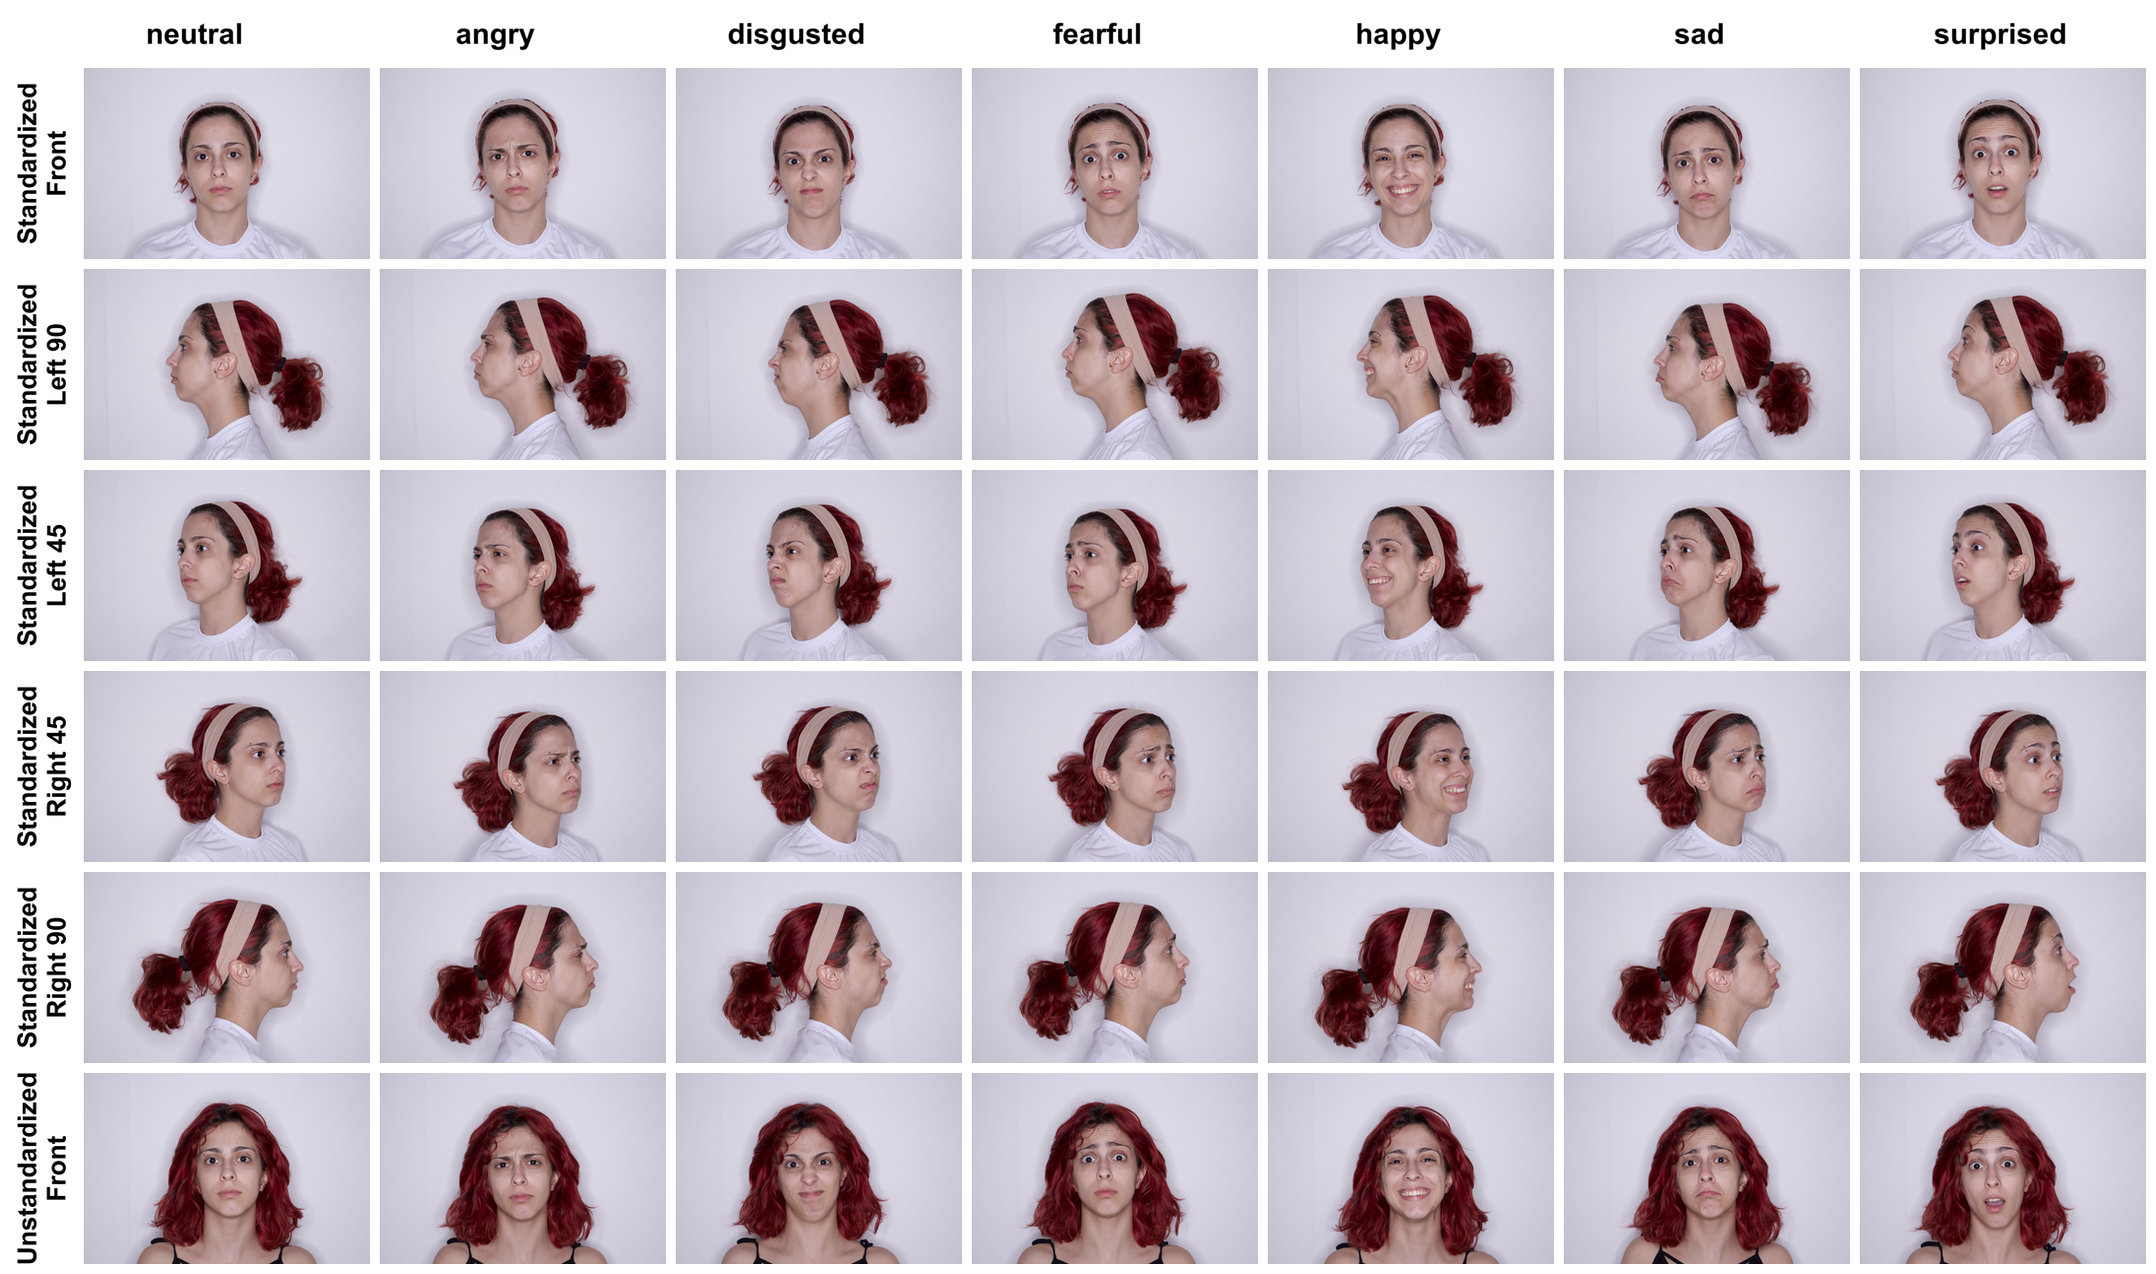
\includegraphics[width=7.19in,height=\textheight,keepaspectratio,alt={A 7x6 grid of pictures of a woman in a white t-shirt with a white headband, showing different angles and expressions. Top labels: neutral, angry, disgusted, fearful, happy, sad, surprised. Side labels: standardized front, standardized left 90 (side profile), standardized left 45 (three-quarter profile), standardized right 45, standardized right 90, unstandardized front.}]{fig/img-examples.png}

}

\end{figure}%

\end{landscape}

\subsubsection{Model self-report}\label{model-self-report}

\textsubscript{Source:
\href{https://ManyFacesTeam.github.io/paper/index.qmd.html}{Article
Notebook}}

For data cleaning, we first downloaded and reshaped the raw data from
Experimentum. In the next step, we ensured that the models'
self-reported gender, race/ethnicity, and units of height and weight
were consistently formatted across labs. For gender and race/ethnicity,
words presented in languages other than English were recoded to be
presented in English (e.g., ``mulher'' to ``female'', ``preta'' to
``Black''). Two members of the research team then classified
self-described race/ethnicity into one of seven categories (checked by a
third team member): ``White'' (n = 84), ``Black'' (n = 4), ``Asian'' (n
= 45), ``Indigenous'' (n = 0), ``MENA'' (Middle Eastern or North
African; n = 15), ``Latine'' (n = 10), or ``Mixed'' (n = 14), where
possible. Descriptions that could not be clearly sorted into these
categories were given ``Ambiguous label'' (n = 7) and non-entries were
recoded as NA (n = 11). Note that the models' original self-reported
phrasing of their gender and race/ethnicity is available in the model
self-report data file included with the image database.

For height, we ensured all data were presented in centimeters, and for
weight, we ensured that all data were presented in kilograms. Models
could report height and weight in metric or imperial units, so we
converted from imperial to metric where required. We also sanity-checked
the reported units, assuming heights \textgreater{} 100 to be in
centimeters and those \textless{} 100 to be in inches, and weights
\textless{} 80 to be in kilograms. Any non-entries of height or weight
for a model was recoded as NA. See Table~\ref{tbl-model-demog} for
descriptive statistics separated by gender, for models whose images are
in the database.

\begin{landscape}

\global\setlength{\Oldarrayrulewidth}{\arrayrulewidth}

\global\setlength{\Oldtabcolsep}{\tabcolsep}

\setlength{\tabcolsep}{2pt}

\renewcommand*{\arraystretch}{1.5}



\providecommand{\ascline}[3]{\noalign{\global\arrayrulewidth #1}\arrayrulecolor[HTML]{#2}\cline{#3}}

\begin{longtable}[c]{|p{0.50in}|p{0.40in}|p{0.40in}|p{0.40in}|p{0.40in}|p{0.40in}|p{0.40in}|p{0.40in}|p{0.40in}|p{0.40in}|p{0.40in}|p{0.40in}|p{0.40in}|p{0.40in}}

\caption{\label{tbl-model-demog}Summary of model age, height, and weight
self-report, separated by gender}

\tabularnewline

\ascline{1.5pt}{666666}{1-14}

\multicolumn{2}{>{\raggedright}m{\dimexpr 0.9in+2\tabcolsep}}{\textcolor[HTML]{000000}{\fontsize{11}{11}\selectfont{\global\setmainfont{Helvetica}{}}}} & \multicolumn{4}{>{\raggedleft}m{\dimexpr 1.6in+6\tabcolsep}}{\textcolor[HTML]{000000}{\fontsize{11}{11}\selectfont{\global\setmainfont{Helvetica}{Age\ (years)}}}} & \multicolumn{4}{>{\raggedleft}m{\dimexpr 1.6in+6\tabcolsep}}{\textcolor[HTML]{000000}{\fontsize{11}{11}\selectfont{\global\setmainfont{Helvetica}{Height\ (cm)}}}} & \multicolumn{4}{>{\raggedleft}m{\dimexpr 1.6in+6\tabcolsep}}{\textcolor[HTML]{000000}{\fontsize{11}{11}\selectfont{\global\setmainfont{Helvetica}{Weight\ (kg)}}}} \\

\ascline{1.5pt}{666666}{1-14}



\multicolumn{1}{>{\raggedright}m{\dimexpr 0.5in+0\tabcolsep}}{\textcolor[HTML]{000000}{\fontsize{11}{11}\selectfont{\global\setmainfont{Helvetica}{gender}}}} & \multicolumn{1}{>{\raggedleft}m{\dimexpr 0.4in+0\tabcolsep}}{\textcolor[HTML]{000000}{\fontsize{11}{11}\selectfont{\global\setmainfont{Helvetica}{n}}}} & \multicolumn{1}{>{\raggedleft}m{\dimexpr 0.4in+0\tabcolsep}}{\textcolor[HTML]{000000}{\fontsize{11}{11}\selectfont{\global\setmainfont{Helvetica}{min}}}} & \multicolumn{1}{>{\raggedleft}m{\dimexpr 0.4in+0\tabcolsep}}{\textcolor[HTML]{000000}{\fontsize{11}{11}\selectfont{\global\setmainfont{Helvetica}{max}}}} & \multicolumn{1}{>{\raggedleft}m{\dimexpr 0.4in+0\tabcolsep}}{\textcolor[HTML]{000000}{\fontsize{11}{11}\selectfont{\global\setmainfont{Helvetica}{M}}}} & \multicolumn{1}{>{\raggedleft}m{\dimexpr 0.4in+0\tabcolsep}}{\textcolor[HTML]{000000}{\fontsize{11}{11}\selectfont{\global\setmainfont{Helvetica}{SD}}}} & \multicolumn{1}{>{\raggedleft}m{\dimexpr 0.4in+0\tabcolsep}}{\textcolor[HTML]{000000}{\fontsize{11}{11}\selectfont{\global\setmainfont{Helvetica}{min}}}} & \multicolumn{1}{>{\raggedleft}m{\dimexpr 0.4in+0\tabcolsep}}{\textcolor[HTML]{000000}{\fontsize{11}{11}\selectfont{\global\setmainfont{Helvetica}{max}}}} & \multicolumn{1}{>{\raggedleft}m{\dimexpr 0.4in+0\tabcolsep}}{\textcolor[HTML]{000000}{\fontsize{11}{11}\selectfont{\global\setmainfont{Helvetica}{M}}}} & \multicolumn{1}{>{\raggedleft}m{\dimexpr 0.4in+0\tabcolsep}}{\textcolor[HTML]{000000}{\fontsize{11}{11}\selectfont{\global\setmainfont{Helvetica}{SD}}}} & \multicolumn{1}{>{\raggedleft}m{\dimexpr 0.4in+0\tabcolsep}}{\textcolor[HTML]{000000}{\fontsize{11}{11}\selectfont{\global\setmainfont{Helvetica}{min}}}} & \multicolumn{1}{>{\raggedleft}m{\dimexpr 0.4in+0\tabcolsep}}{\textcolor[HTML]{000000}{\fontsize{11}{11}\selectfont{\global\setmainfont{Helvetica}{max}}}} & \multicolumn{1}{>{\raggedleft}m{\dimexpr 0.4in+0\tabcolsep}}{\textcolor[HTML]{000000}{\fontsize{11}{11}\selectfont{\global\setmainfont{Helvetica}{M}}}} & \multicolumn{1}{>{\raggedleft}m{\dimexpr 0.4in+0\tabcolsep}}{\textcolor[HTML]{000000}{\fontsize{11}{11}\selectfont{\global\setmainfont{Helvetica}{SD}}}} \\

\ascline{1.5pt}{666666}{1-14}\endfirsthead 

\ascline{1.5pt}{666666}{1-14}

\multicolumn{2}{>{\raggedright}m{\dimexpr 0.9in+2\tabcolsep}}{\textcolor[HTML]{000000}{\fontsize{11}{11}\selectfont{\global\setmainfont{Helvetica}{}}}} & \multicolumn{4}{>{\raggedleft}m{\dimexpr 1.6in+6\tabcolsep}}{\textcolor[HTML]{000000}{\fontsize{11}{11}\selectfont{\global\setmainfont{Helvetica}{Age\ (years)}}}} & \multicolumn{4}{>{\raggedleft}m{\dimexpr 1.6in+6\tabcolsep}}{\textcolor[HTML]{000000}{\fontsize{11}{11}\selectfont{\global\setmainfont{Helvetica}{Height\ (cm)}}}} & \multicolumn{4}{>{\raggedleft}m{\dimexpr 1.6in+6\tabcolsep}}{\textcolor[HTML]{000000}{\fontsize{11}{11}\selectfont{\global\setmainfont{Helvetica}{Weight\ (kg)}}}} \\

\ascline{1.5pt}{666666}{1-14}



\multicolumn{1}{>{\raggedright}m{\dimexpr 0.5in+0\tabcolsep}}{\textcolor[HTML]{000000}{\fontsize{11}{11}\selectfont{\global\setmainfont{Helvetica}{gender}}}} & \multicolumn{1}{>{\raggedleft}m{\dimexpr 0.4in+0\tabcolsep}}{\textcolor[HTML]{000000}{\fontsize{11}{11}\selectfont{\global\setmainfont{Helvetica}{n}}}} & \multicolumn{1}{>{\raggedleft}m{\dimexpr 0.4in+0\tabcolsep}}{\textcolor[HTML]{000000}{\fontsize{11}{11}\selectfont{\global\setmainfont{Helvetica}{min}}}} & \multicolumn{1}{>{\raggedleft}m{\dimexpr 0.4in+0\tabcolsep}}{\textcolor[HTML]{000000}{\fontsize{11}{11}\selectfont{\global\setmainfont{Helvetica}{max}}}} & \multicolumn{1}{>{\raggedleft}m{\dimexpr 0.4in+0\tabcolsep}}{\textcolor[HTML]{000000}{\fontsize{11}{11}\selectfont{\global\setmainfont{Helvetica}{M}}}} & \multicolumn{1}{>{\raggedleft}m{\dimexpr 0.4in+0\tabcolsep}}{\textcolor[HTML]{000000}{\fontsize{11}{11}\selectfont{\global\setmainfont{Helvetica}{SD}}}} & \multicolumn{1}{>{\raggedleft}m{\dimexpr 0.4in+0\tabcolsep}}{\textcolor[HTML]{000000}{\fontsize{11}{11}\selectfont{\global\setmainfont{Helvetica}{min}}}} & \multicolumn{1}{>{\raggedleft}m{\dimexpr 0.4in+0\tabcolsep}}{\textcolor[HTML]{000000}{\fontsize{11}{11}\selectfont{\global\setmainfont{Helvetica}{max}}}} & \multicolumn{1}{>{\raggedleft}m{\dimexpr 0.4in+0\tabcolsep}}{\textcolor[HTML]{000000}{\fontsize{11}{11}\selectfont{\global\setmainfont{Helvetica}{M}}}} & \multicolumn{1}{>{\raggedleft}m{\dimexpr 0.4in+0\tabcolsep}}{\textcolor[HTML]{000000}{\fontsize{11}{11}\selectfont{\global\setmainfont{Helvetica}{SD}}}} & \multicolumn{1}{>{\raggedleft}m{\dimexpr 0.4in+0\tabcolsep}}{\textcolor[HTML]{000000}{\fontsize{11}{11}\selectfont{\global\setmainfont{Helvetica}{min}}}} & \multicolumn{1}{>{\raggedleft}m{\dimexpr 0.4in+0\tabcolsep}}{\textcolor[HTML]{000000}{\fontsize{11}{11}\selectfont{\global\setmainfont{Helvetica}{max}}}} & \multicolumn{1}{>{\raggedleft}m{\dimexpr 0.4in+0\tabcolsep}}{\textcolor[HTML]{000000}{\fontsize{11}{11}\selectfont{\global\setmainfont{Helvetica}{M}}}} & \multicolumn{1}{>{\raggedleft}m{\dimexpr 0.4in+0\tabcolsep}}{\textcolor[HTML]{000000}{\fontsize{11}{11}\selectfont{\global\setmainfont{Helvetica}{SD}}}} \\

\ascline{1.5pt}{666666}{1-14}\endhead



\multicolumn{1}{>{\raggedright}m{\dimexpr 0.5in+0\tabcolsep}}{\textcolor[HTML]{000000}{\fontsize{11}{11}\selectfont{\global\setmainfont{Helvetica}{female}}}} & \multicolumn{1}{>{\raggedleft}m{\dimexpr 0.4in+0\tabcolsep}}{\textcolor[HTML]{000000}{\fontsize{11}{11}\selectfont{\global\setmainfont{Helvetica}{106}}}} & \multicolumn{1}{>{\raggedleft}m{\dimexpr 0.4in+0\tabcolsep}}{\textcolor[HTML]{000000}{\fontsize{11}{11}\selectfont{\global\setmainfont{Helvetica}{18.0}}}} & \multicolumn{1}{>{\raggedleft}m{\dimexpr 0.4in+0\tabcolsep}}{\textcolor[HTML]{000000}{\fontsize{11}{11}\selectfont{\global\setmainfont{Helvetica}{65.0}}}} & \multicolumn{1}{>{\raggedleft}m{\dimexpr 0.4in+0\tabcolsep}}{\textcolor[HTML]{000000}{\fontsize{11}{11}\selectfont{\global\setmainfont{Helvetica}{27.3}}}} & \multicolumn{1}{>{\raggedleft}m{\dimexpr 0.4in+0\tabcolsep}}{\textcolor[HTML]{000000}{\fontsize{11}{11}\selectfont{\global\setmainfont{Helvetica}{9.9}}}} & \multicolumn{1}{>{\raggedleft}m{\dimexpr 0.4in+0\tabcolsep}}{\textcolor[HTML]{000000}{\fontsize{11}{11}\selectfont{\global\setmainfont{Helvetica}{149.0}}}} & \multicolumn{1}{>{\raggedleft}m{\dimexpr 0.4in+0\tabcolsep}}{\textcolor[HTML]{000000}{\fontsize{11}{11}\selectfont{\global\setmainfont{Helvetica}{180.0}}}} & \multicolumn{1}{>{\raggedleft}m{\dimexpr 0.4in+0\tabcolsep}}{\textcolor[HTML]{000000}{\fontsize{11}{11}\selectfont{\global\setmainfont{Helvetica}{165.4}}}} & \multicolumn{1}{>{\raggedleft}m{\dimexpr 0.4in+0\tabcolsep}}{\textcolor[HTML]{000000}{\fontsize{11}{11}\selectfont{\global\setmainfont{Helvetica}{6.9}}}} & \multicolumn{1}{>{\raggedleft}m{\dimexpr 0.4in+0\tabcolsep}}{\textcolor[HTML]{000000}{\fontsize{11}{11}\selectfont{\global\setmainfont{Helvetica}{37.0}}}} & \multicolumn{1}{>{\raggedleft}m{\dimexpr 0.4in+0\tabcolsep}}{\textcolor[HTML]{000000}{\fontsize{11}{11}\selectfont{\global\setmainfont{Helvetica}{108.9}}}} & \multicolumn{1}{>{\raggedleft}m{\dimexpr 0.4in+0\tabcolsep}}{\textcolor[HTML]{000000}{\fontsize{11}{11}\selectfont{\global\setmainfont{Helvetica}{63.4}}}} & \multicolumn{1}{>{\raggedleft}m{\dimexpr 0.4in+0\tabcolsep}}{\textcolor[HTML]{000000}{\fontsize{11}{11}\selectfont{\global\setmainfont{Helvetica}{13.9}}}} \\





\multicolumn{1}{>{\raggedright}m{\dimexpr 0.5in+0\tabcolsep}}{\textcolor[HTML]{000000}{\fontsize{11}{11}\selectfont{\global\setmainfont{Helvetica}{male}}}} & \multicolumn{1}{>{\raggedleft}m{\dimexpr 0.4in+0\tabcolsep}}{\textcolor[HTML]{000000}{\fontsize{11}{11}\selectfont{\global\setmainfont{Helvetica}{75}}}} & \multicolumn{1}{>{\raggedleft}m{\dimexpr 0.4in+0\tabcolsep}}{\textcolor[HTML]{000000}{\fontsize{11}{11}\selectfont{\global\setmainfont{Helvetica}{18.0}}}} & \multicolumn{1}{>{\raggedleft}m{\dimexpr 0.4in+0\tabcolsep}}{\textcolor[HTML]{000000}{\fontsize{11}{11}\selectfont{\global\setmainfont{Helvetica}{80.0}}}} & \multicolumn{1}{>{\raggedleft}m{\dimexpr 0.4in+0\tabcolsep}}{\textcolor[HTML]{000000}{\fontsize{11}{11}\selectfont{\global\setmainfont{Helvetica}{26.9}}}} & \multicolumn{1}{>{\raggedleft}m{\dimexpr 0.4in+0\tabcolsep}}{\textcolor[HTML]{000000}{\fontsize{11}{11}\selectfont{\global\setmainfont{Helvetica}{9.5}}}} & \multicolumn{1}{>{\raggedleft}m{\dimexpr 0.4in+0\tabcolsep}}{\textcolor[HTML]{000000}{\fontsize{11}{11}\selectfont{\global\setmainfont{Helvetica}{163.0}}}} & \multicolumn{1}{>{\raggedleft}m{\dimexpr 0.4in+0\tabcolsep}}{\textcolor[HTML]{000000}{\fontsize{11}{11}\selectfont{\global\setmainfont{Helvetica}{193.0}}}} & \multicolumn{1}{>{\raggedleft}m{\dimexpr 0.4in+0\tabcolsep}}{\textcolor[HTML]{000000}{\fontsize{11}{11}\selectfont{\global\setmainfont{Helvetica}{178.5}}}} & \multicolumn{1}{>{\raggedleft}m{\dimexpr 0.4in+0\tabcolsep}}{\textcolor[HTML]{000000}{\fontsize{11}{11}\selectfont{\global\setmainfont{Helvetica}{7.6}}}} & \multicolumn{1}{>{\raggedleft}m{\dimexpr 0.4in+0\tabcolsep}}{\textcolor[HTML]{000000}{\fontsize{11}{11}\selectfont{\global\setmainfont{Helvetica}{54.0}}}} & \multicolumn{1}{>{\raggedleft}m{\dimexpr 0.4in+0\tabcolsep}}{\textcolor[HTML]{000000}{\fontsize{11}{11}\selectfont{\global\setmainfont{Helvetica}{130.0}}}} & \multicolumn{1}{>{\raggedleft}m{\dimexpr 0.4in+0\tabcolsep}}{\textcolor[HTML]{000000}{\fontsize{11}{11}\selectfont{\global\setmainfont{Helvetica}{79.9}}}} & \multicolumn{1}{>{\raggedleft}m{\dimexpr 0.4in+0\tabcolsep}}{\textcolor[HTML]{000000}{\fontsize{11}{11}\selectfont{\global\setmainfont{Helvetica}{16.7}}}} \\





\multicolumn{1}{>{\raggedright}m{\dimexpr 0.5in+0\tabcolsep}}{\textcolor[HTML]{000000}{\fontsize{11}{11}\selectfont{\global\setmainfont{Helvetica}{non-binary}}}} & \multicolumn{1}{>{\raggedleft}m{\dimexpr 0.4in+0\tabcolsep}}{\textcolor[HTML]{000000}{\fontsize{11}{11}\selectfont{\global\setmainfont{Helvetica}{7}}}} & \multicolumn{1}{>{\raggedleft}m{\dimexpr 0.4in+0\tabcolsep}}{\textcolor[HTML]{000000}{\fontsize{11}{11}\selectfont{\global\setmainfont{Helvetica}{19.0}}}} & \multicolumn{1}{>{\raggedleft}m{\dimexpr 0.4in+0\tabcolsep}}{\textcolor[HTML]{000000}{\fontsize{11}{11}\selectfont{\global\setmainfont{Helvetica}{37.0}}}} & \multicolumn{1}{>{\raggedleft}m{\dimexpr 0.4in+0\tabcolsep}}{\textcolor[HTML]{000000}{\fontsize{11}{11}\selectfont{\global\setmainfont{Helvetica}{24.7}}}} & \multicolumn{1}{>{\raggedleft}m{\dimexpr 0.4in+0\tabcolsep}}{\textcolor[HTML]{000000}{\fontsize{11}{11}\selectfont{\global\setmainfont{Helvetica}{5.8}}}} & \multicolumn{1}{>{\raggedleft}m{\dimexpr 0.4in+0\tabcolsep}}{\textcolor[HTML]{000000}{\fontsize{11}{11}\selectfont{\global\setmainfont{Helvetica}{165.0}}}} & \multicolumn{1}{>{\raggedleft}m{\dimexpr 0.4in+0\tabcolsep}}{\textcolor[HTML]{000000}{\fontsize{11}{11}\selectfont{\global\setmainfont{Helvetica}{201.0}}}} & \multicolumn{1}{>{\raggedleft}m{\dimexpr 0.4in+0\tabcolsep}}{\textcolor[HTML]{000000}{\fontsize{11}{11}\selectfont{\global\setmainfont{Helvetica}{175.0}}}} & \multicolumn{1}{>{\raggedleft}m{\dimexpr 0.4in+0\tabcolsep}}{\textcolor[HTML]{000000}{\fontsize{11}{11}\selectfont{\global\setmainfont{Helvetica}{12.0}}}} & \multicolumn{1}{>{\raggedleft}m{\dimexpr 0.4in+0\tabcolsep}}{\textcolor[HTML]{000000}{\fontsize{11}{11}\selectfont{\global\setmainfont{Helvetica}{59.0}}}} & \multicolumn{1}{>{\raggedleft}m{\dimexpr 0.4in+0\tabcolsep}}{\textcolor[HTML]{000000}{\fontsize{11}{11}\selectfont{\global\setmainfont{Helvetica}{110.0}}}} & \multicolumn{1}{>{\raggedleft}m{\dimexpr 0.4in+0\tabcolsep}}{\textcolor[HTML]{000000}{\fontsize{11}{11}\selectfont{\global\setmainfont{Helvetica}{74.1}}}} & \multicolumn{1}{>{\raggedleft}m{\dimexpr 0.4in+0\tabcolsep}}{\textcolor[HTML]{000000}{\fontsize{11}{11}\selectfont{\global\setmainfont{Helvetica}{16.9}}}} \\





\multicolumn{1}{>{\raggedright}m{\dimexpr 0.5in+0\tabcolsep}}{\textcolor[HTML]{000000}{\fontsize{11}{11}\selectfont{\global\setmainfont{Helvetica}{NA}}}} & \multicolumn{1}{>{\raggedleft}m{\dimexpr 0.4in+0\tabcolsep}}{\textcolor[HTML]{000000}{\fontsize{11}{11}\selectfont{\global\setmainfont{Helvetica}{2}}}} & \multicolumn{1}{>{\raggedleft}m{\dimexpr 0.4in+0\tabcolsep}}{\textcolor[HTML]{000000}{\fontsize{11}{11}\selectfont{\global\setmainfont{Helvetica}{27.0}}}} & \multicolumn{1}{>{\raggedleft}m{\dimexpr 0.4in+0\tabcolsep}}{\textcolor[HTML]{000000}{\fontsize{11}{11}\selectfont{\global\setmainfont{Helvetica}{30.0}}}} & \multicolumn{1}{>{\raggedleft}m{\dimexpr 0.4in+0\tabcolsep}}{\textcolor[HTML]{000000}{\fontsize{11}{11}\selectfont{\global\setmainfont{Helvetica}{28.5}}}} & \multicolumn{1}{>{\raggedleft}m{\dimexpr 0.4in+0\tabcolsep}}{\textcolor[HTML]{000000}{\fontsize{11}{11}\selectfont{\global\setmainfont{Helvetica}{2.1}}}} & \multicolumn{1}{>{\raggedleft}m{\dimexpr 0.4in+0\tabcolsep}}{\textcolor[HTML]{000000}{\fontsize{11}{11}\selectfont{\global\setmainfont{Helvetica}{167.0}}}} & \multicolumn{1}{>{\raggedleft}m{\dimexpr 0.4in+0\tabcolsep}}{\textcolor[HTML]{000000}{\fontsize{11}{11}\selectfont{\global\setmainfont{Helvetica}{169.0}}}} & \multicolumn{1}{>{\raggedleft}m{\dimexpr 0.4in+0\tabcolsep}}{\textcolor[HTML]{000000}{\fontsize{11}{11}\selectfont{\global\setmainfont{Helvetica}{168.0}}}} & \multicolumn{1}{>{\raggedleft}m{\dimexpr 0.4in+0\tabcolsep}}{\textcolor[HTML]{000000}{\fontsize{11}{11}\selectfont{\global\setmainfont{Helvetica}{1.4}}}} & \multicolumn{1}{>{\raggedleft}m{\dimexpr 0.4in+0\tabcolsep}}{\textcolor[HTML]{000000}{\fontsize{11}{11}\selectfont{\global\setmainfont{Helvetica}{60.0}}}} & \multicolumn{1}{>{\raggedleft}m{\dimexpr 0.4in+0\tabcolsep}}{\textcolor[HTML]{000000}{\fontsize{11}{11}\selectfont{\global\setmainfont{Helvetica}{61.0}}}} & \multicolumn{1}{>{\raggedleft}m{\dimexpr 0.4in+0\tabcolsep}}{\textcolor[HTML]{000000}{\fontsize{11}{11}\selectfont{\global\setmainfont{Helvetica}{60.5}}}} & \multicolumn{1}{>{\raggedleft}m{\dimexpr 0.4in+0\tabcolsep}}{\textcolor[HTML]{000000}{\fontsize{11}{11}\selectfont{\global\setmainfont{Helvetica}{0.7}}}} \\

\ascline{1.5pt}{666666}{1-14}


\end{longtable}

\arrayrulecolor[HTML]{000000}

\global\setlength{\arrayrulewidth}{\Oldarrayrulewidth}

\global\setlength{\tabcolsep}{\Oldtabcolsep}

\renewcommand*{\arraystretch}{1}

\emph{Note.} See Figure~\ref{fig-model-age} in SM for histograms.

\end{landscape}

\section{Phase 2: Validation/norming
data}\label{phase-2-validationnorming-data}

We next obtained subjective ratings of a subset of the photos
(front-facing) to validate the emotion expressions (their perceived
emotion category and intensity) and collect norming data on central
social perceptions, namely perceived attractiveness, dominance,
trustworthiness, gender-typicality, memorability, and age. We chose
these ratings due to their central importance in the person perception,
face recognition, and emotion perception literatures (e.g., Bainbridge
et al., 2013; Jack et al., 2016; Oosterhof \& Todorov, 2008; Perrett,
2017; Sutherland et al., 2013). We preregistered this study on the Open
Science Framework (\url{https://osf.io/4d5v9}) in April 2025.

\subsection{Method}\label{method-1}

\subsubsection{Image processing}\label{image-processing}

RAW images were processed using webmorphR (DeBruine et al., 2022), which
facilitates scriptable processing of images using imagemagick
(ImageMagick Studio LLC, 2024) (a full script of the processing steps is
available at \url{https://github.com/ManyFacesTeam/imgprep}). Briefly,

\begin{itemize}
\tightlist
\item
  Each face was delineated using the Face++ automatic face detection
  algorithm (see \url{https://www.faceplusplus.com/}) to generate a
  106-point template.
\item
  All images were resized to 1000w by 1500h pixels to standardize size
  (two different RAW formats were used, which resulted in two different
  image sizes)
\item
  The median RGB colour value of a 100×100 pixel patch at the upper left
  corner was calculated to fill in any edges from alignment.
\item
  The image was repositioned and cropped (not rotated or resized) such
  that

  \begin{itemize}
  \tightlist
  \item
    The image size was 675w by 900h pixel
  \item
    point 71 (between the eyes) was relocated to position {[}.5w, .4h{]}
  \end{itemize}
\item
  This aligned image was saved as a lossless PNG using imagemagick
  default settings (e.g., sRGB colour space).
\item
  A white balance correction was applied to the resulting images,
  calculated from the mean RGB values in the 25x25 pixel top-right
  corner patch (white background) \footnote{We did not fully
    colour-calibrate the images here (see Discussion) but future
    researchers may wish to do so.}
\item
  These images were converted to JPEGs with a quality setting of 75 to
  reduce file size and enable interoperability across browsers and
  devices for stimulus display online. These processed images are
  available alongside the full set of images in the image database. The
  full set of RAW images were converted to 50\% size and saved in
  high-quality JPEG format because the RAW file sizes exceeded the
  archive capacity.
\end{itemize}

\protect\phantomsection\label{cell-fig-img-processing}
\begin{figure}[H]

\caption{\label{fig-img-processing}Image processing steps: (A) the raw
image, (B) the image automatically delineated and cropped to a standard
alignment, (C) white balance correction.}

\centering{

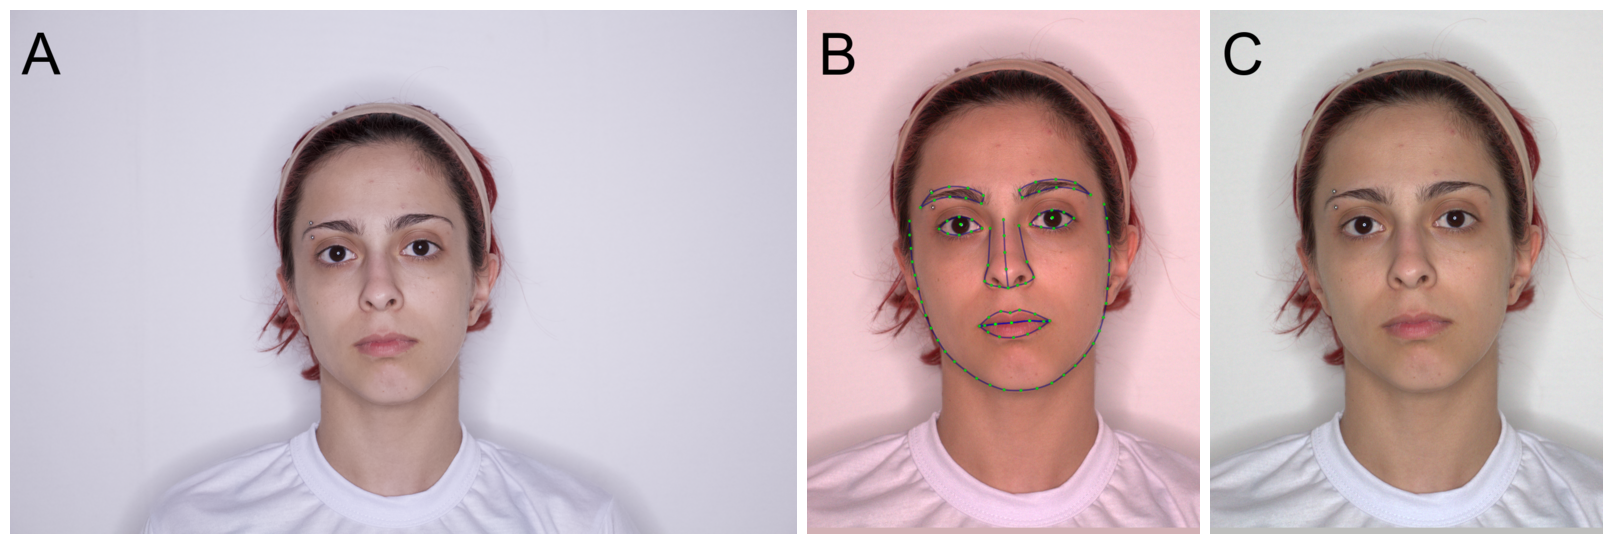
\includegraphics[width=5.38in,height=\textheight,keepaspectratio]{fig/img-processing.png}

}

\end{figure}%

\textsubscript{Source:
\href{https://ManyFacesTeam.github.io/paper/index.qmd.html}{Article
Notebook}}

\subsubsection{Stimuli}\label{stimuli}

The number of stimuli was determined by the number of models recruited
across the 20 research labs and how many models posed for each image
type. The maximum number of targets per image type was 205\footnote{The
  preregistration mis-stated the total number of models, rather than the
  maximum number of images, to be 205. The total number of models was
  211}, meaning each rater saw up to 205 stimuli. We obtained ratings of
the front-facing standardized neutral (n = 205), unstandardized neutral
(n = 177), standardized angry (n = 187), standardized disgusted (n =
184), standardized fearful (n = 175), standardized happy (n = 199),
standardized sad (n = 183), and standardized surprised (n = 184) images.
Note that these numbers of stimuli are higher than the number of stimuli
available in the database, as not all models consented to database
inclusion.

\begin{landscape}

\begin{figure}[H]

\caption{\label{fig-stim-examples}An example of each type of stimulus.}

\centering{

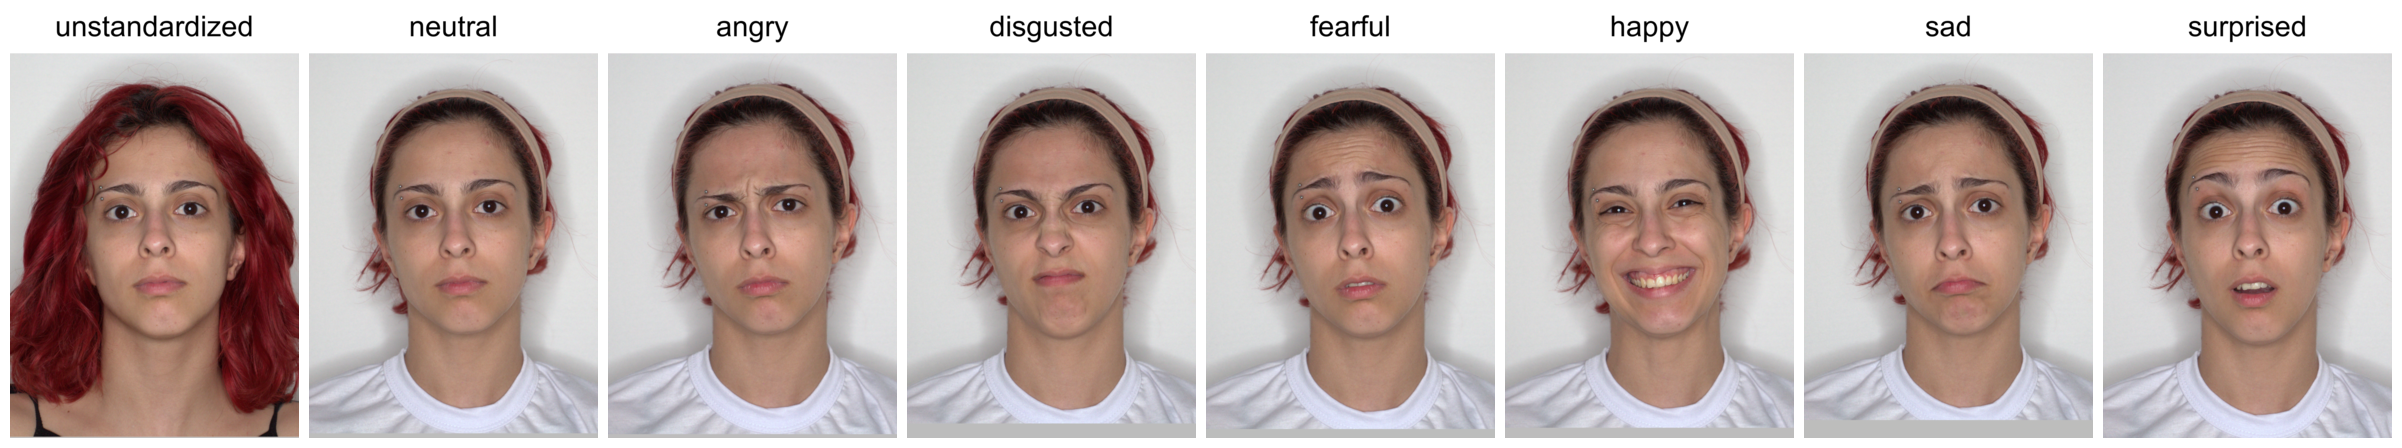
\includegraphics[width=8.01in,height=\textheight,keepaspectratio,alt={Example face images for the 8 types of stimuli: unstandardized neutral, standardized neutral, angry, disgusted, fearful, happy, sad, and surprised}]{fig/stim-types.png}

}

\end{figure}%

\end{landscape}

\subsubsection{Attention check stimuli}\label{attention-check-stimuli}

Additionally, we created stimuli for attention checks. These were white
images with the same size and aspect ratio as the face stimuli, but
contained only the written instruction to choose a specific response,
(e.g., `Choose ``fear''\,' or `Choose ``3''\,').

\subsubsection{Measures}\label{measures}

\paragraph{Standardized neutral faces}\label{standardized-neutral-faces}

\subparagraph{Trait ratings}\label{trait-ratings}

We obtained ratings of faces' attractiveness, dominance,
trustworthiness, memorability, and gender-typicality (``How attractive
{[}dominant, trustworthy, memorable, gender-typical{]} does this person
look?''). Ratings were on scales ranging from 1 (\emph{not at all}) to 7
(\emph{very}).

\subparagraph{Age ratings}\label{age-ratings}

We obtained ratings of faces' perceived age (``How old does this person
look?''), with responses collected in 5-year ranges/brackets (i.e.,
16-20, 21-25, \ldots, 76-80, 81+).

\paragraph{Unstandardized neutral
faces}\label{unstandardized-neutral-faces}

\subparagraph{Trait ratings}\label{trait-ratings-1}

We obtained ratings of faces' attractiveness, dominance, and
trustworthiness on scales ranging from 1 (\emph{not at all}) to 7
(\emph{very}).

\paragraph{Standardized emotional
faces}\label{standardized-emotional-faces}

\subparagraph{Emotion categorization}\label{emotion-categorization}

We obtained impressions of the emotion each person was expressing
(``What emotion is this person expressing?''), choosing one from:
\emph{anger, disgust, fear, happiness, sadness, surprise, other}. Here,
raters categorized a counterbalanced mixture of expressions (from one of
six counterbalanced conditions) rather than faces all showing the same
expression. The 201 identities with emotion expression images were
divided into six groups of up to 34 images, and each counterbalanced
condition showed a different emotion expression for each of the six
groups, such that no identity was shown more than once to each rater.
Since not all identities had all six emotion expressions, the number of
images in each counterbalanced condition ranged from 179 to 193.

\subparagraph{Emotion intensity
ratings}\label{emotion-intensity-ratings}

We obtained ratings of how intensely faces expressed each intended
emotion (``How intensely is this person expressing anger {[}disgust,
fear, happiness, sadness, surprise{]}?'') from 1 (\emph{not at all}) to
7 (\emph{very}). Here, raters only rated all faces showing one emotion
expression (e.g., all angry faces) and rated the intensity only of the
intended expression (e.g., angry faces only rated on anger intensity).

\subsubsection{Procedure}\label{procedure-1}

We collected ratings via Experimentum (DeBruine et al., 2020); a
structure file for the exact experimental setup is available on Zenodo
(\url{https://doi.org/10.5281/zenodo.22707036}). After a brief
introduction to the study and online informed consent, each participant
(rater) was randomly allocated to one of the ratings (e.g., rating all
205 standardized neutral faces on how memorable they look). All
available faces were displayed one at a time, in a randomized order for
each rater. The question/prompt and response scale remained visible at
the top of the screen, above the photo throughout the study. The study
automatically progressed to the next trial once the rater responded by
clicking on the response scale. There was no time limit to provide a
response. We included seven attention checks embedded in the study,
which directed raters to provide a specific response.

Following rating or categorizing all stimuli, raters self-reported their
gender, age, race/ethnicity, country of residence, and device type used
for the study (desktop, laptop, tablet, mobile). They also completed an
honesty/attention check question, asking them if they engaged with the
study seriously, with assurance of payment regardless of response
(choosing from ``no, I was not really paying attention'' and ``yes, I
tried to give my authentic first impressions'').

We recruited a gender-balanced sample of fluent English-speaking raters
through Prolific (we included no other screening criteria). We collected
all data in May 2025\footnote{This was slightly later than preregistered
  (April 2025), due to pretesting and study setup delays. Note that we
  also planned to collect perceived race/ethnicity data, but decided
  against this, due to the regional specificity of race/ethnicity
  labels.}.

\subsubsection{Participants}\label{participants}

We aimed to collect 100 raters per rating condition to achieve stable
averages and allow for exclusions (Hehman et al., 2025), totalling 2100
raters. Altogether, 2115 raters completed the study and received
compensation in line with Prolific's guidelines. See Results for
exclusions and demographics of the final sample.

\subsection{Results}\label{results-1}

We present here only the results for ratings of images of models who
agreed to be included in the database, rather than all images raters
saw.

\subsubsection{Data cleaning and
exclusions}\label{data-cleaning-and-exclusions}

In the raters' demographic questionnaire, we standardized participants'
recording of their race/ethnicity similarly to the models by recoding
their inputs into one of seven categories (``White'', ``Black'',
``Asian'', ``Indigenous/Pacific Islander'', ``MENA'' (Middle Eastern or
North African), ``Latine'', or ``Mixed''), or as ``Ambiguous'' when this
was not possible. Any non-entries were recoded as NA. Raters' original
self-reported labels are available in the data shared on Github.

A total of 2115 raters completed 2158 rating or categorization tasks. We
found that some raters did not complete all trials in tasks, some raters
completed more than one task, and some raters completed more than the
maximum number of trials in a task (likely by restarting the study or
bypassing the back button block). Therefore, we removed incomplete tasks
from our data, retained raters' first complete tasks, and filtered our
duplicate trials by keeping only raters' first ratings for a duplicated
trial. After these exclusions, and before implementing the
pre-registered plan for data exclusions, we had complete and clean data
from 1936 raters.

Our pre-registered plan for data exclusions included removing raters who
gave overly consistent responses, committed overly fast responses,
self-reported not taking the study seriously when asked whether or not
they completed the study authentically, and failed attention checks. In
total, we excluded 49 raters for our pre-registered reasons for data
exclusions. Table~\ref{tbl-exclusions} in the Supplementary Material
(SM) shows the number of raters we excluded for each of our reasons.

We defined overly consistent responses as those raters who responded to
at least 90\% of trials identically. During agreement analyses (see
Agreement Indicators for the Ratings, below), we found that 4 additional
raters only gave two unique responses across all trials and also
excluded these as overly consistent. We defined overly fast responses as
those raters whose median reaction time fell below the 1st percentile of
the overall distribution of median reaction times (see
Figure~\ref{fig-rt-distribution} in SM for the distribution of median
reaction times). For our attention checks, the threshold for inclusion
was to accurately complete six or more attention checks (i.e.,
participants were excluded if they failed more than one of the checks).
Lastly, participants were excluded based on a self-reported honesty
check, i.e., if they reported not taking the study seriously rather than
taking it authentically. After these exclusions, we had 1887 raters in
our sample (with between 80 and 114 raters per rating task; see
Table~\ref{tbl-raters-per-task} in SM for the number of raters per
task).

Anonymous data, along with data cleaning and analysis scripts are
available on Github
(\url{https://github.com/ManyFacesTeam/rating-data}).

\subsubsection{Rater demographics}\label{rater-demographics}

\textsubscript{Source:
\href{https://ManyFacesTeam.github.io/paper/index.qmd.html}{Article
Notebook}}

We collected the following demographic data from our raters (N = 1652
provided data): Age, gender, residence, ethnicity, and devices on which
the ratings were completed. Raters were predominantly younger adults (M
age = 35.33 years, SD = 12.57; see Figure~\ref{fig-age} in SM for
histogram), male (n = 879; 768 female, 5 nonbinary), and Black (n = 920;
577 White, 69 Asian, 34 Latine, 28 mixed, 5 MENA; 3 Indigenous or
Pacific Islander; 16 ambiguously labelled or unreported), and spanned
world regions (primarily Africa, Americas, and Europe; see
Table~\ref{tbl-raters-country} in SM for breakdown by country).
Participants completed the study on a variety of devices (739 laptop,
461 desktop computer, 415 mobile phone, 37 tablet).

\subsubsection{Agreement indicators for the
ratings}\label{agreement-indicators-for-the-ratings}

In the first step, we calculated intraclass correlation coefficients
{[}ICC(2,k){]} for each of the ratings. The average reliability across
raters was excellent for ratings of standardized and unstandardized
neutral faces' attractiveness, dominance, and trustworthiness,
standardized neutral faces' gender-typicality, and standardized
emotional faces' emotion intensity (.84 ≤ ICC ≤ .98), but poorer for
ratings of standardized neutral faces' memorability (ICC = .59; see
Table~\ref{tbl-icc} in SM).

Next, we examined the number of raters required for ratings to reach
stable levels of reliability defined as ICC(2,k) values of 0.75 (see
Figure~\ref{fig-icc-cos}). Emotion intensity and attractiveness ratings
stabilized with the fewest participants (reaching a median ICC(2,k) of
0.75 at 10 raters for happiness, disgust, and surprise; 20 for anger,
fear, sadness, and attractiveness) and were also the only ratings to
exceed a median ICC(2,k) of 0.90. Ratings for dominance,
trustworthiness, and gender-typicality stabilized at larger samples
(reached a median ICC(2,k) of 0.75 with 40-60 raters), whereas ratings
for memorability did not reach these levels of reliability.

\begin{figure}[H]

\caption{\label{fig-icc-cos}Corridors of stability for ICC}

\centering{

\centering{

\pandocbounded{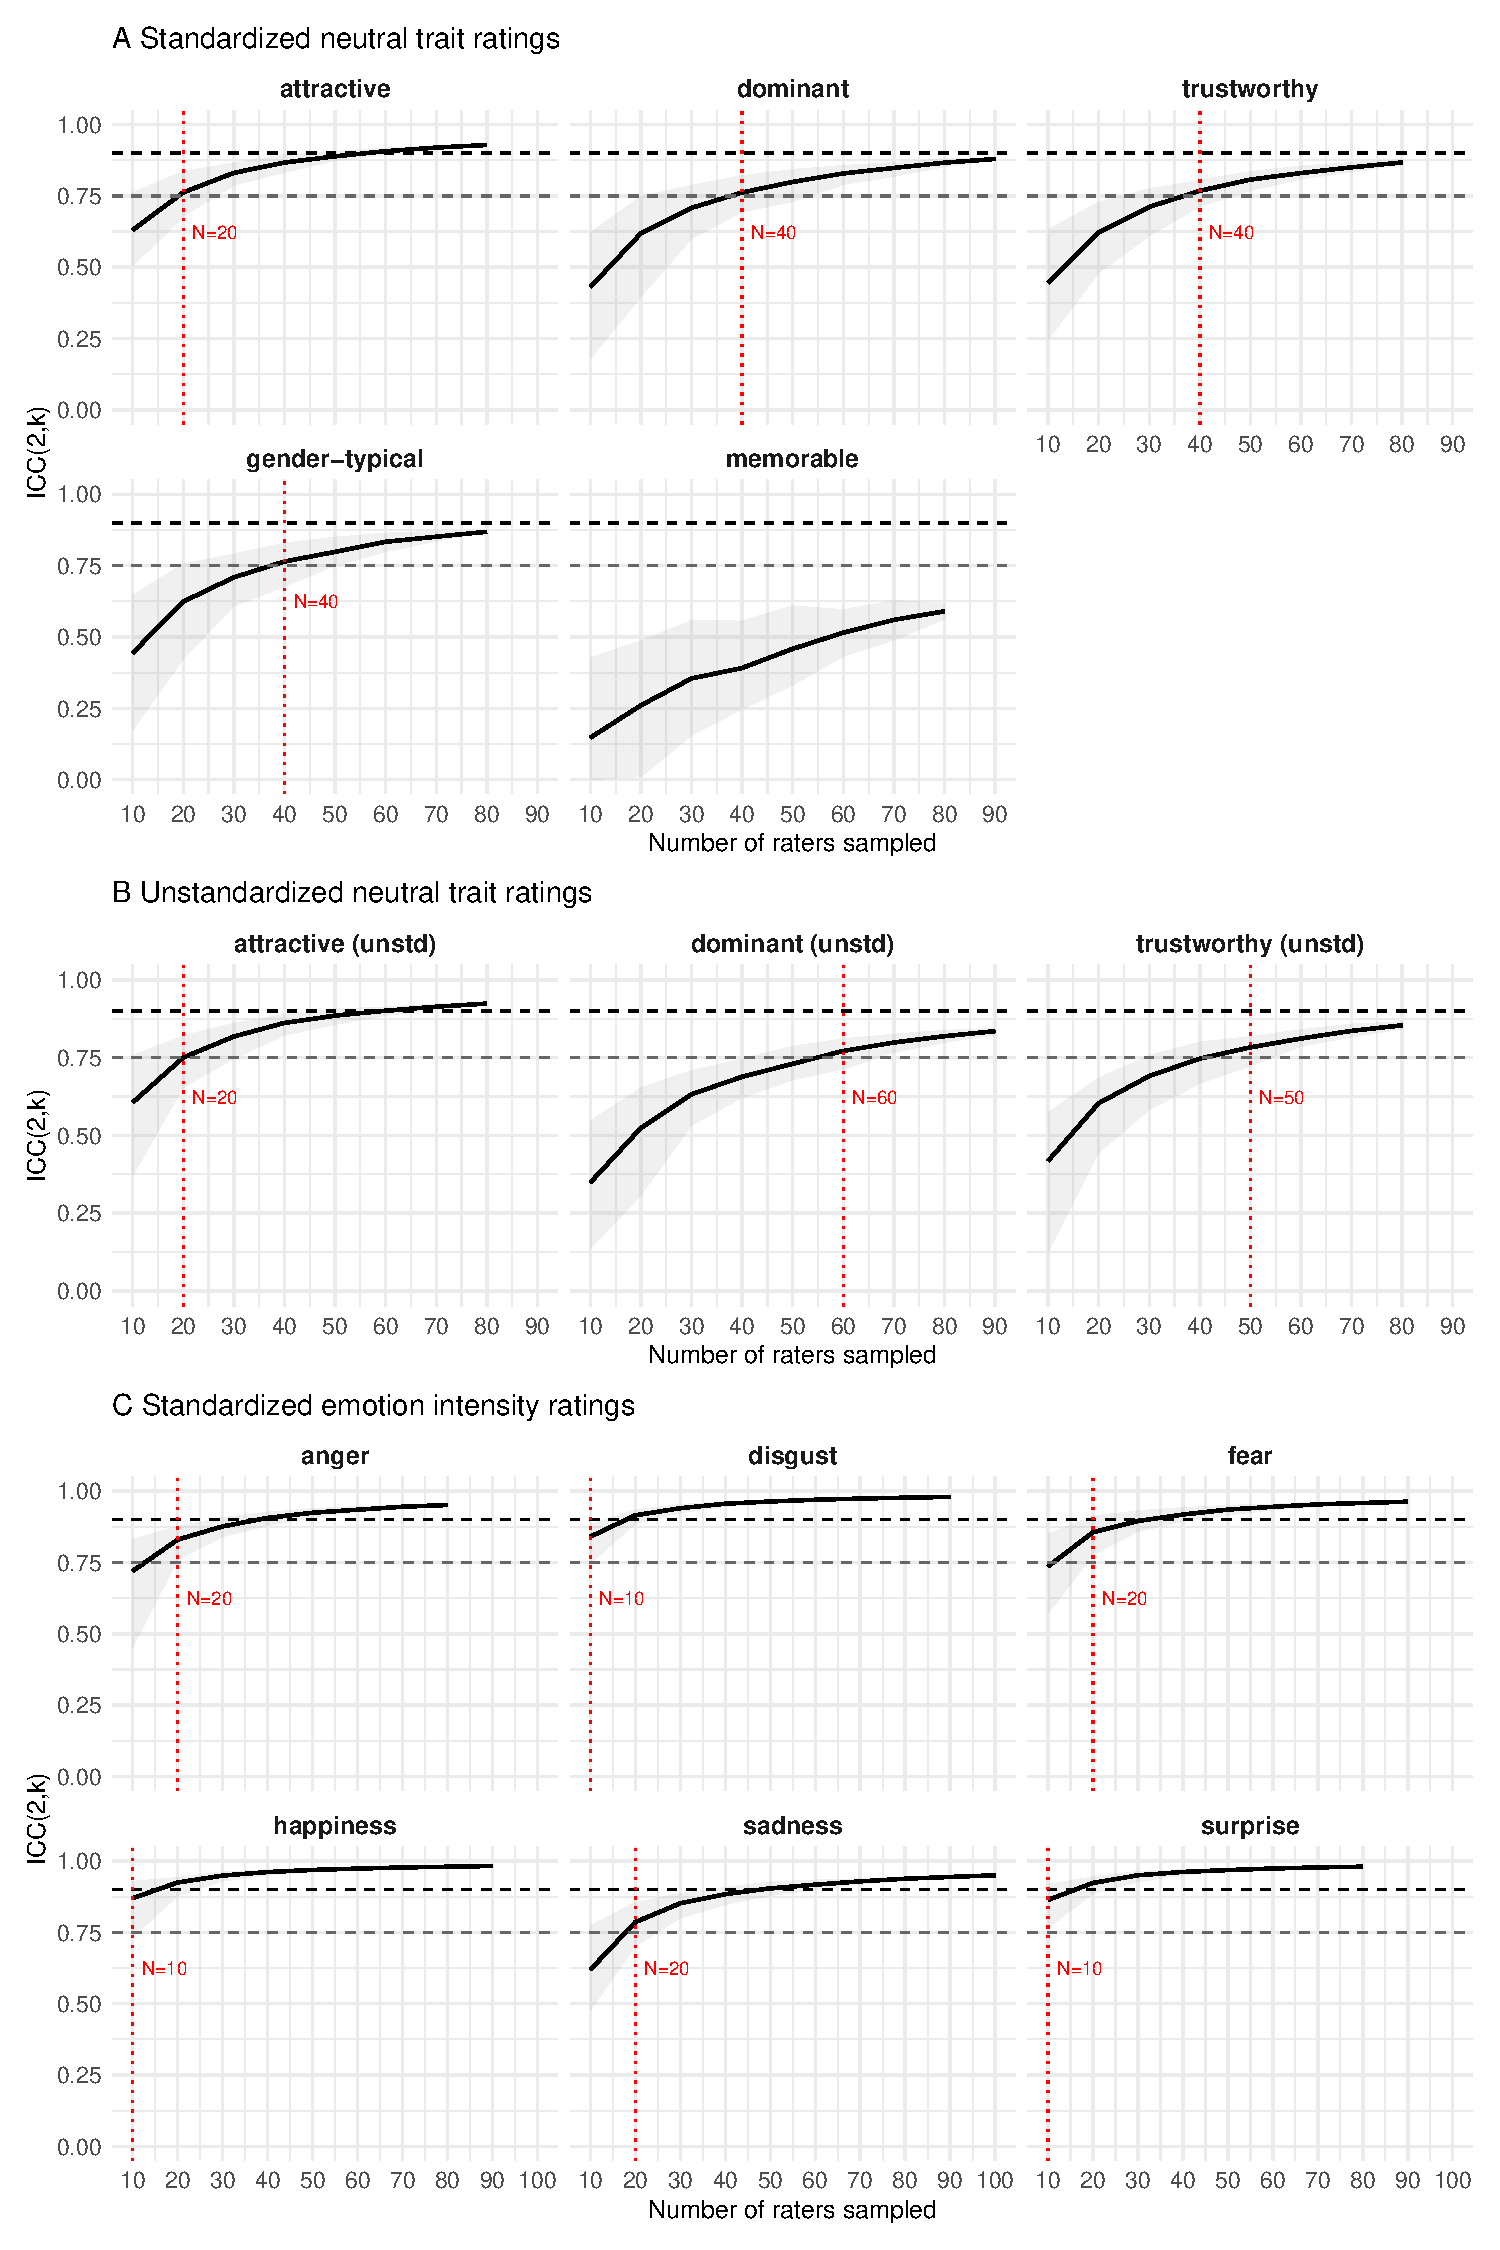
\includegraphics[keepaspectratio]{index_files/figure-pdf/fig-icc-cos-1.pdf}}

}

\subcaption{\label{fig-icc-cos}Note. Dashed horizontal lines indicate
ICC(2,k) of 0.75 and 0.90, respectively.}

}

\end{figure}%

\textsubscript{Source:
\href{https://ManyFacesTeam.github.io/paper/index.qmd.html}{Article
Notebook}}

To further check inter-rater agreement, we used both Cronbach's alpha
(α) and McDonald's omega total (ωt; see Table~\ref{tbl-icc} in SM). For
attractiveness, dominance, trustworthiness, gender-typicality, and
emotion intensity ratings, both measures indicated excellent inter-rater
agreement (.88 ≤ α ≤ .99; .90 ≤ ωt ≤ .99). For ratings of memorability,
α was lower (0.67), suggesting reduced inter-rater agreement. ωt for
memorability was substantially higher (0.87), suggesting better
agreement under the assumption that raters varied in how consistently
they judged memorability, a pattern consistent with the lower ICC
observed for this trait.

\subsubsection{Points of stability}\label{points-of-stability}

To determine the number of raters required for stable ratings, we
computed the point of stability (Hehman et al., 2025), defined as the
smallest sample size at which 95\% of resampled means fall within a
corridor of stability of ±0.5 points and do not again exceed
it.\footnote{Note that we declared stability when the \emph{upper} bound
  crossed inside the threshold, whereas Hehman and colleagues declare
  stability when the lower/nearer bound crosses inside the threshold.}
As shown in Figure~\ref{fig-pos}, the ratings of standardized images
reached stability between 36 and 45 raters, the ratings of
unstandardized images between 37 and 41 raters, and emotion intensity
ratings of standardized emotional faces between 29 and 50 raters.

\begin{figure}[H]

\caption{\label{fig-pos}Points of stability for ratings}

\centering{

\centering{

\pandocbounded{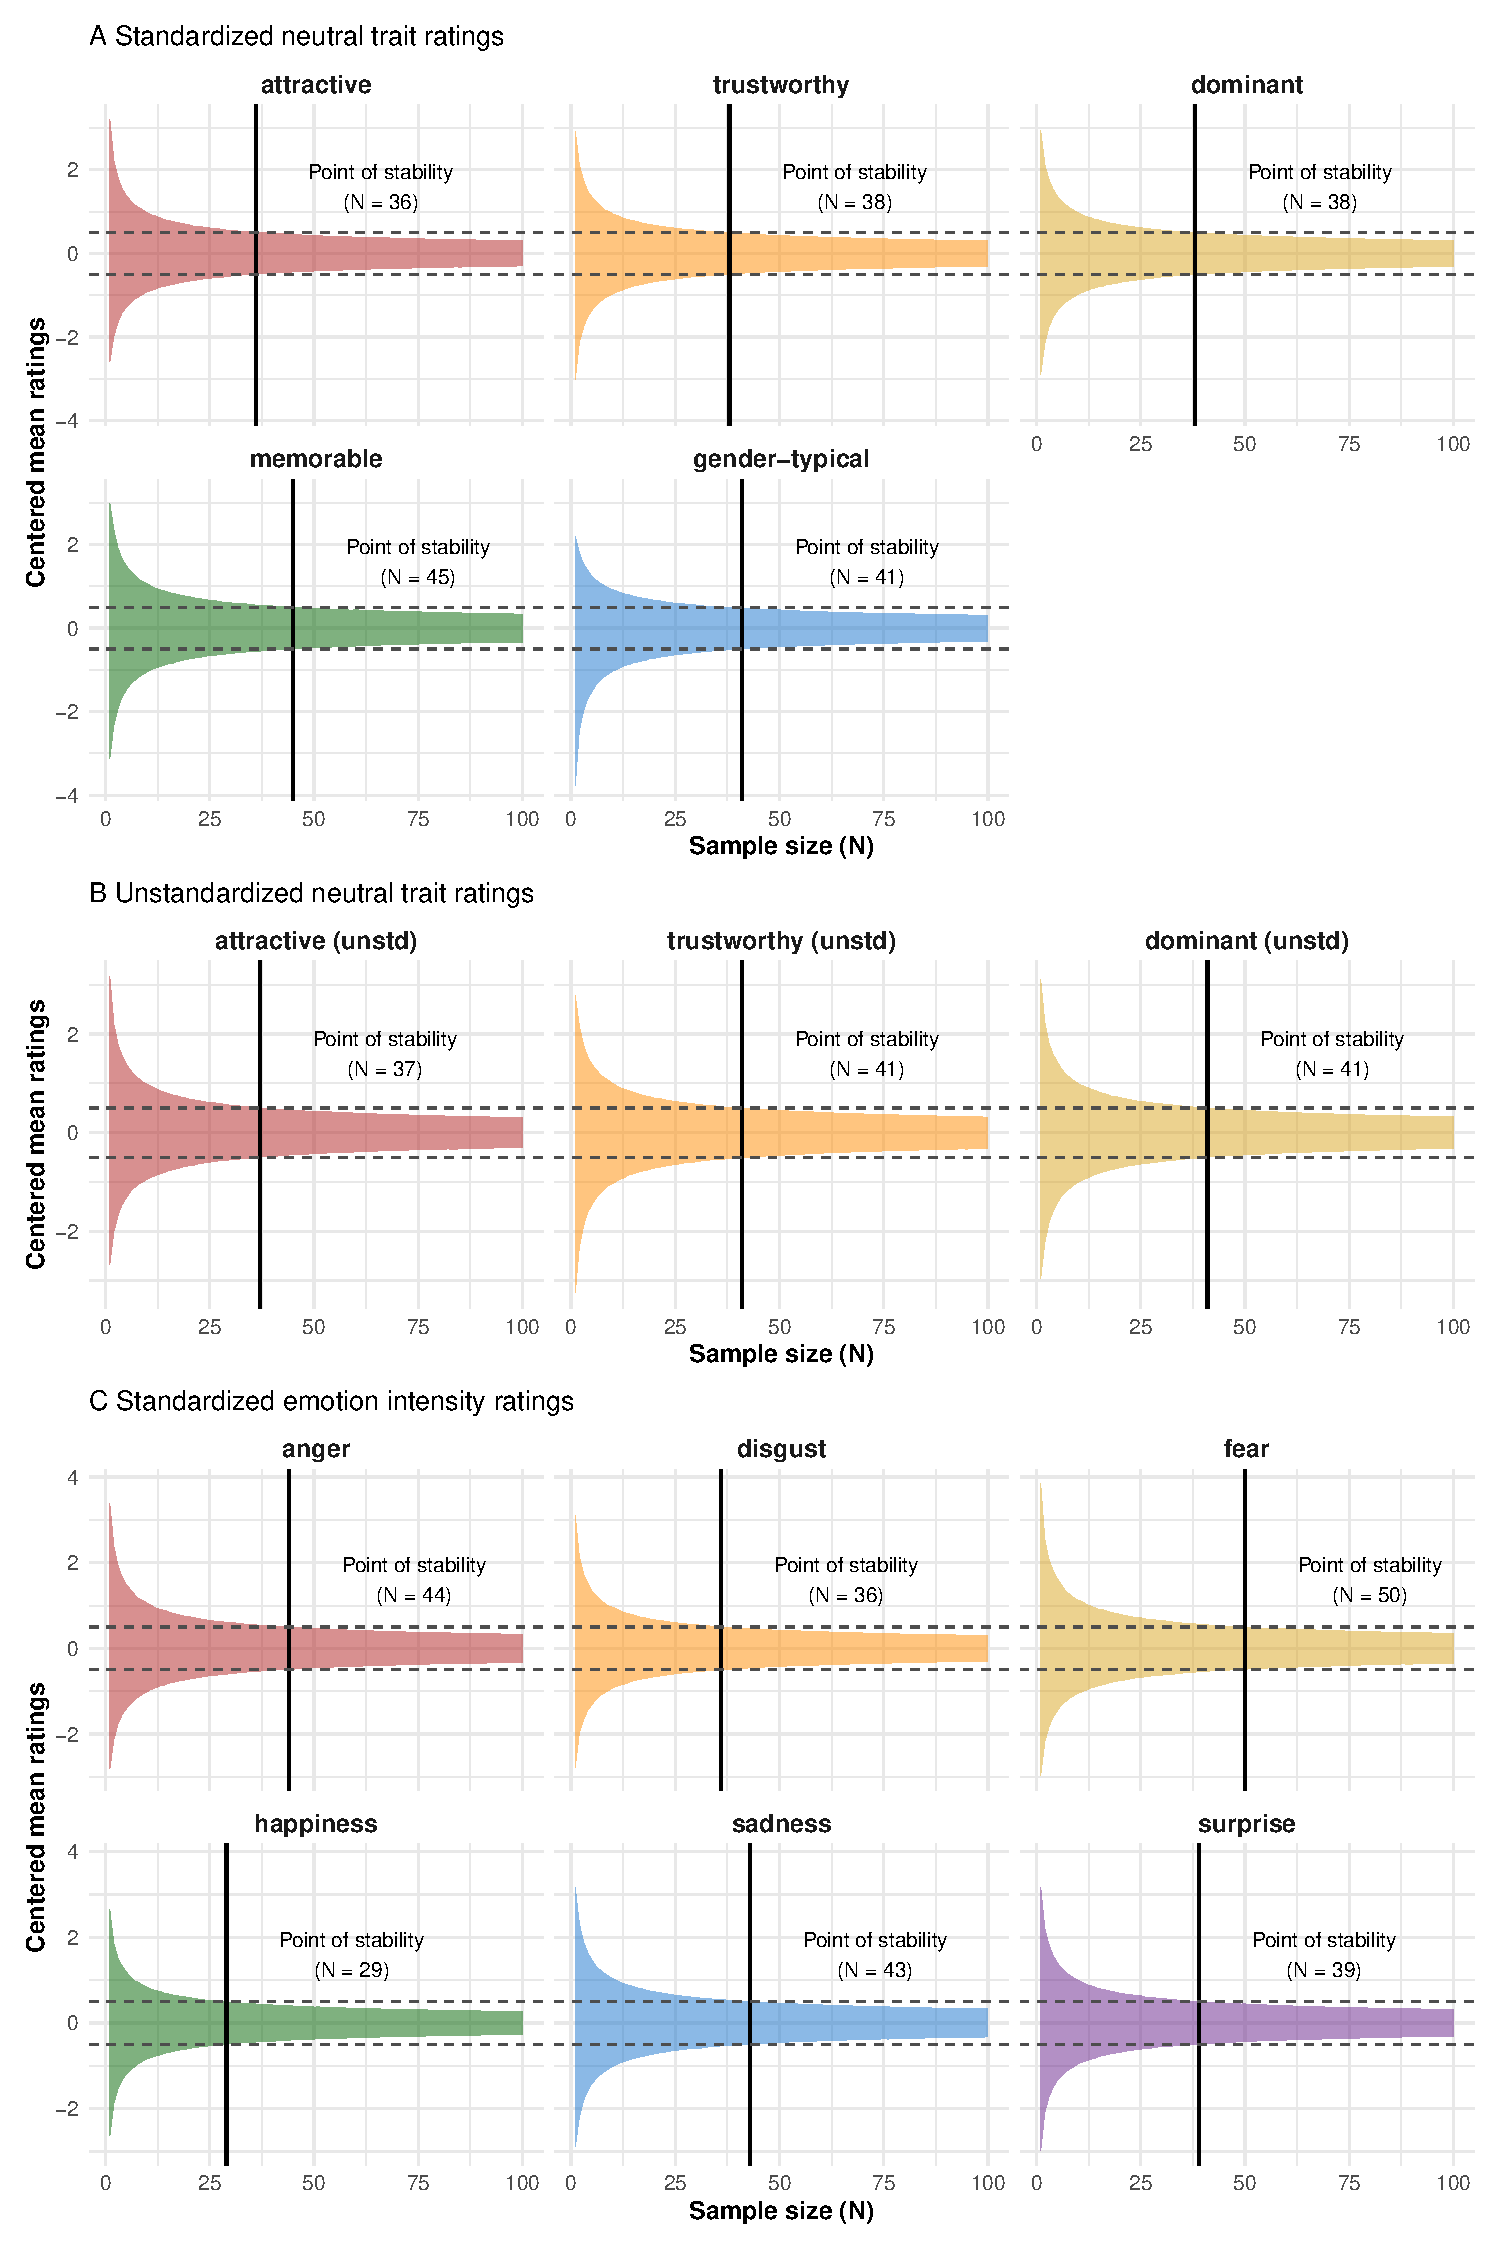
\includegraphics[keepaspectratio]{index_files/figure-pdf/fig-pos-1.pdf}}

}

\subcaption{\label{fig-pos}Note. Dashed horizontal lines indicate
corridor of stability at +/- 0.5 points. Vertical lines indicate point
of stability.}

}

\end{figure}%

\textsubscript{Source:
\href{https://ManyFacesTeam.github.io/paper/index.qmd.html}{Article
Notebook}}

\subsubsection{Descriptive statistics}\label{descriptive-statistics}

In this section, we report the descriptive statistics for trait ratings
of the standardized and unstandardized neutral images, the emotion
categorizations and emotion intensity ratings of the standardized
emotional images, and the perceived ages of the models (standardized
neutral images).

\paragraph{Standardized and unstandardized neutral trait
ratings}\label{standardized-and-unstandardized-neutral-trait-ratings}

For standardized neutral faces, trustworthiness, dominance, and
memorability ratings were approximately normally distributed and showed
similar patterns of central tendency and variance. In contrast,
attractiveness ratings were somewhat right-skewed, whereas
gender-typicality ratings were left-skewed (see
Figure~\ref{fig-neu-hist}). For unstandardized neutral faces, patterns
for attractiveness and dominance were similar to those for standardized
neutral faces, but trustworthiness ratings showed slight left skew.

\textsubscript{Source:
\href{https://ManyFacesTeam.github.io/paper/index.qmd.html}{Article
Notebook}}

\begin{figure}[H]

\caption{\label{fig-neu-hist}Histograms and descriptive statistics for
trait ratings of standardized and unstandardized neutral faces}

\centering{

\centering{

\pandocbounded{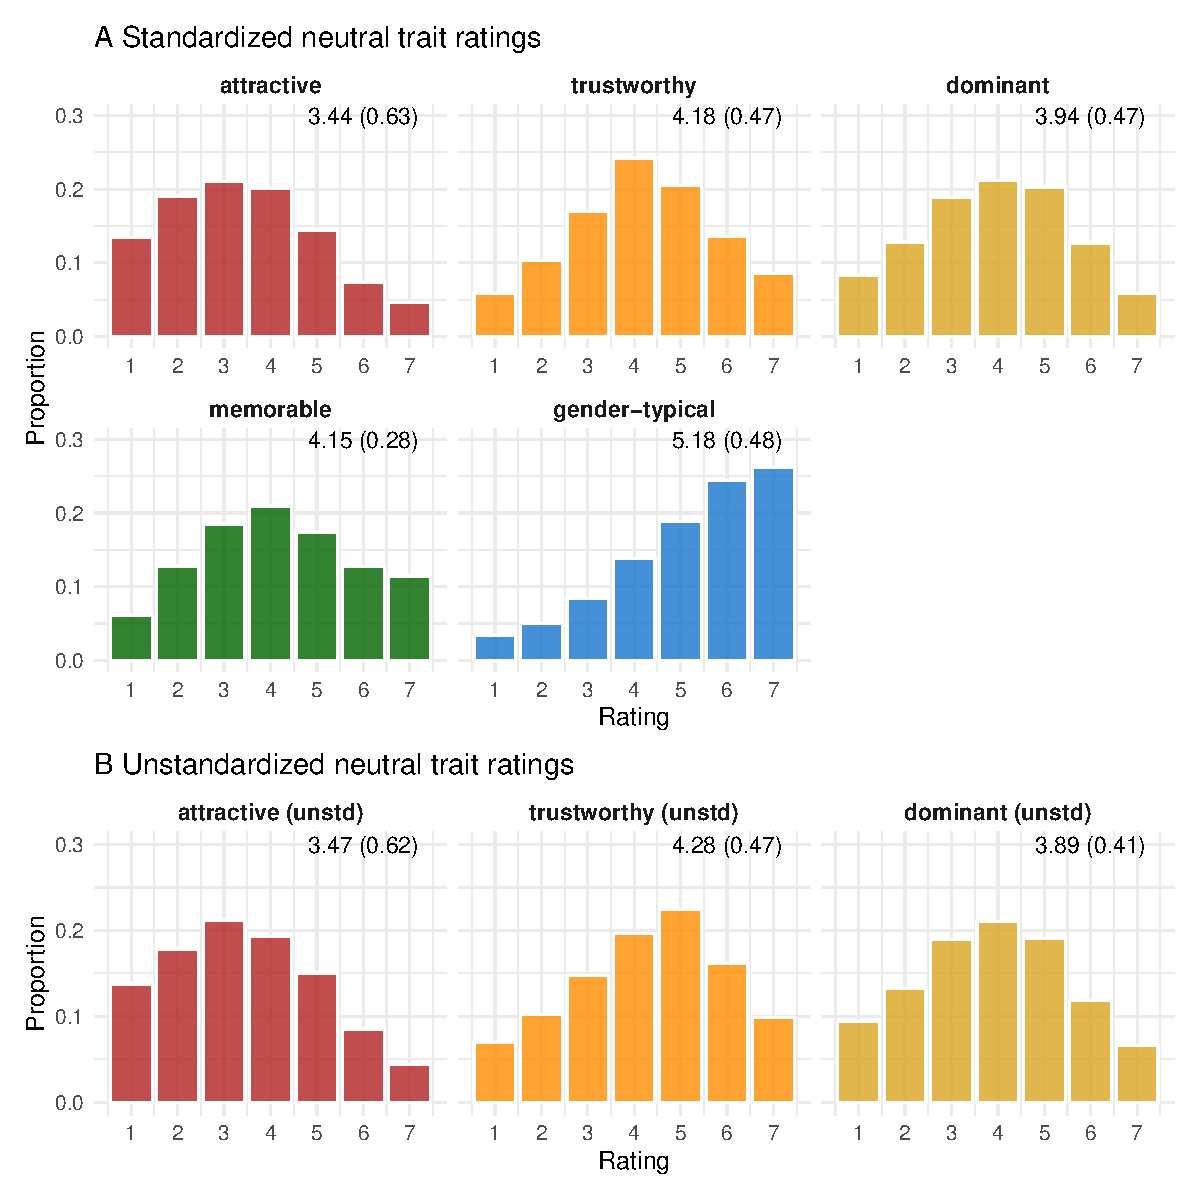
\includegraphics[keepaspectratio]{index_files/figure-pdf/fig-neu-hist-1.pdf}}

}

\subcaption{\label{fig-neu-hist}Note. Values in top right of each panel
represent M (SD).}

}

\end{figure}%

\textsubscript{Source:
\href{https://ManyFacesTeam.github.io/paper/index.qmd.html}{Article
Notebook}}

\paragraph{Emotion categorization and intensity
ratings}\label{emotion-categorization-and-intensity-ratings}

Next, we explored raters' emotion categorizations and perceived emotion
intensity expressed by our models. Raters' categorizations generally
aligned with the models' expression of emotion, with the greatest
alignment observed for expression of happiness, and the least for fear,
with fearful faces most often perceived as expressing surprise rather
than fear (see Figure~\ref{fig-emo-freq}, Table~\ref{tbl-emo-desc} in
SM).

\textsubscript{Source:
\href{https://ManyFacesTeam.github.io/paper/index.qmd.html}{Article
Notebook}}

\protect\phantomsection\label{cell-fig-emo-freq}
\begin{figure}[H]

\caption{\label{fig-emo-freq}Emotion categorization frequencies}

\centering{

\pandocbounded{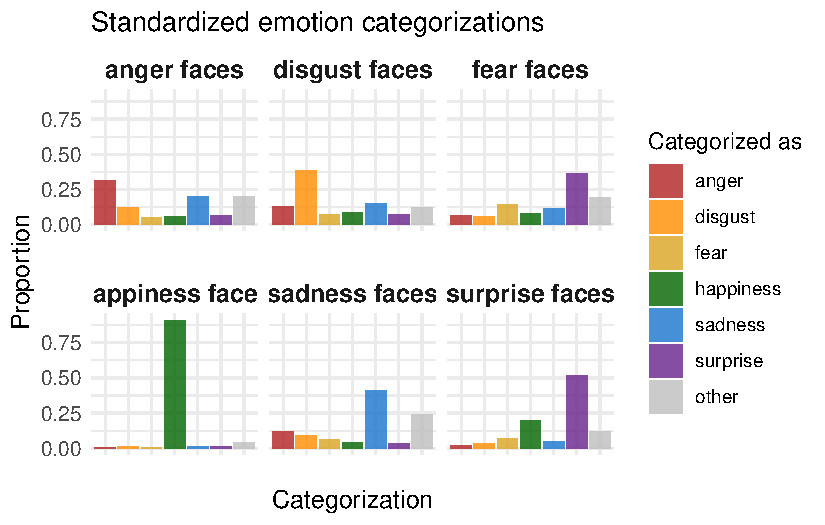
\includegraphics[keepaspectratio]{index_files/figure-pdf/fig-emo-freq-1.pdf}}

}

\end{figure}%

\textsubscript{Source:
\href{https://ManyFacesTeam.github.io/paper/index.qmd.html}{Article
Notebook}}

Next, we calculated the average ratings of emotion intensity for each
emotion (Figure~\ref{fig-intensity-hist}). These ratings were very
similar, on average, between the different emotions except for
happiness, which was rated with greater intensity than all other
emotions. On average, these ratings were located around the middle of
the 7-point scale.

\textsubscript{Source:
\href{https://ManyFacesTeam.github.io/paper/index.qmd.html}{Article
Notebook}}

\begin{figure}[H]

\caption{\label{fig-intensity-hist}Histograms of emotion intensity
ratings}

\centering{

\centering{

\pandocbounded{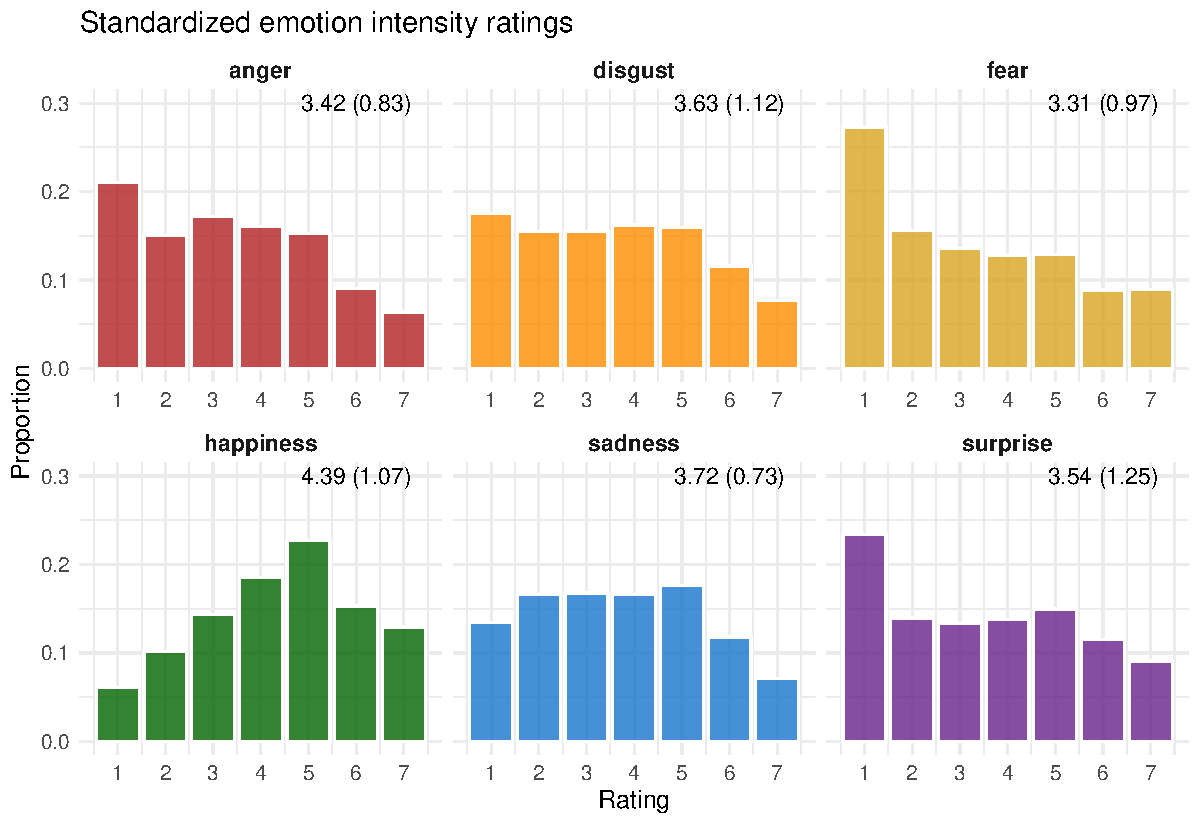
\includegraphics[keepaspectratio]{index_files/figure-pdf/fig-intensity-hist-1.pdf}}

}

\subcaption{\label{fig-intensity-hist}Note. Values in top right of each
panel represent M (SD).}

}

\end{figure}%

\textsubscript{Source:
\href{https://ManyFacesTeam.github.io/paper/index.qmd.html}{Article
Notebook}}

\paragraph{Perceived age}\label{perceived-age}

\textsubscript{Source:
\href{https://ManyFacesTeam.github.io/paper/index.qmd.html}{Article
Notebook}}

The distribution of raters' perceptions of models' ages is shown in
Figure~\ref{fig-age-hist} (see Figure~\ref{fig-model-age} in SM for
actual age). The most chosen age across raters and models was 26--30
years. The correlation between models' mode perceived age and actual age
was strong,\emph{r}(182) = 0.86, p \textless{} 0.001.

\protect\phantomsection\label{cell-fig-age-hist}
\begin{figure}[H]

\caption{\label{fig-age-hist}Histogram of perceived age}

\centering{

\pandocbounded{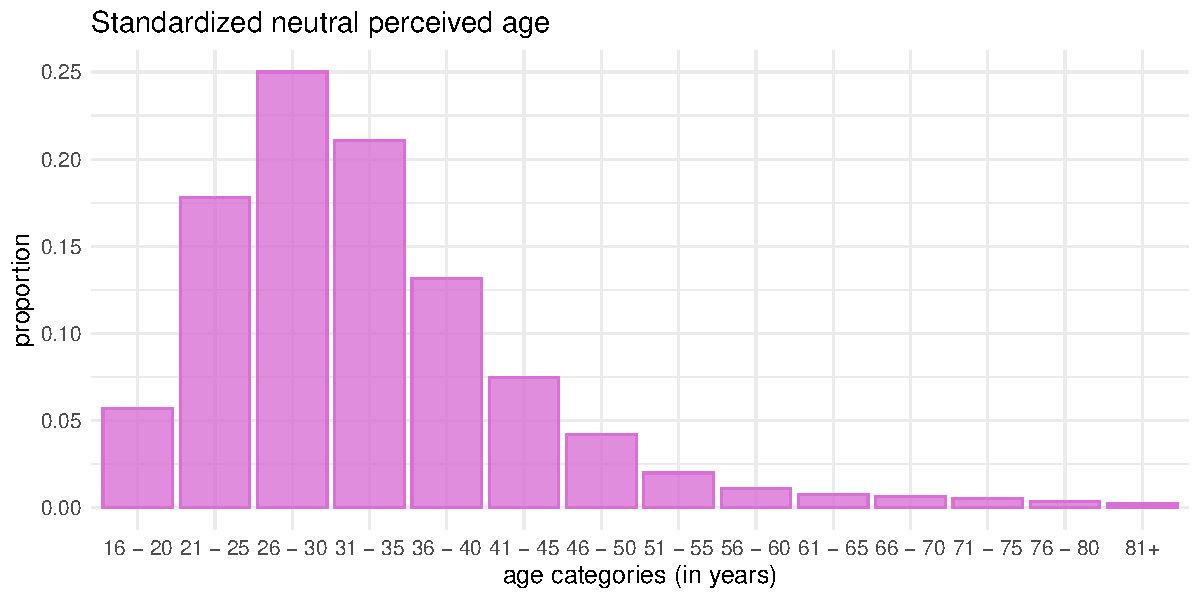
\includegraphics[keepaspectratio]{index_files/figure-pdf/fig-age-hist-1.pdf}}

}

\end{figure}%

\textsubscript{Source:
\href{https://ManyFacesTeam.github.io/paper/index.qmd.html}{Article
Notebook}}

\section{Discussion}\label{discussion}

\subsection{The value of the current
work}\label{the-value-of-the-current-work}

This first ManyFaces team project provides a unique contribution to the
current landscape of face image datasets by developing a comprehensive,
transparent, open, and accessible protocol
(\url{https://doi.org/10.5281/zenodo.22707036}) to collect and process
face images. Following this, we additionally introduce a database
(accessed via ReShare \textbf{LINK}, subject to agreement to Terms of
Use) that provides a diverse face image stimulus set in terms of models'
geographic location and image variety (appearance standardization,
viewing angle, and facial expression). The diversity of images within
the database makes it potentially useful to address a variety of
research questions in multiple areas of psychology (e.g., face
recognition, emotion perception) and beyond.

Additionally, the database need not remain fixed: Other researchers can
follow the provided procedures and add to the database, further
increasing its sample size and diversity (e.g., in terms of model age,
ethnicity, culture, and geographic location). Researchers wishing to
contribute to the database can contact the ManyFaces team (via
\href{mailto:ManyFacesDatabase@gmail.com}{\nolinkurl{ManyFacesDatabase@gmail.com}})
to have their images linked on our database landing page
(\url{https://doi.org/10.5281/zenodo.22707036}; future additions will
therefore have a distributed database structure, enabling greater
flexibility than a single, centrally managed database structure). The
protocol can also serve as a template for researchers interested in
collecting stimulus images, in terms of highlighting the kinds of
details that need to be considered and documented.

The data associated with the images are also valuable. First, we
collected ground-truth information from models, namely their
self-reported demographic information (age, gender, ethnicity), body
measurements (height, weight), and information about any makeup worn in
the photos and any experiences or procedures which may have affected
their facial appearance, each of which is useful for various kinds of
research questions. The validation/norming data we collected
(\url{https://github.com/ManyFacesTeam/rating-data}) also provide a
useful starting point for researchers interested in using the images,
for example enabling researchers to choose subsets of images most suited
to address their research questions.

\subsection{Validation/norming ratings}\label{validationnorming-ratings}

The patterns of ratings we obtained largely converge with published
research. The higher intensity ratings of happiness expressions,
compared to the other expressions, is similar to previous findings. For
example, faces expressing happiness in the Radboud Faces Database were
rated higher in intensity than most expressions (except fear) and higher
in clarity than all other expressions (Langner et al., 2010), and happy
faces in the Karolinska Directed Emotional Faces were similarly rated
higher in intensity than most expressions (but not differing
significantly from disgust or surprise, Goeleven et al., 2008)
Additionally, we found emotion recognition to be highest for happy
expressions. These results align with other emotion recognition research
using posed facial expressions of emotion. For example, emotion
recognition was highest for faces expressing happiness in the Radboud
Faces Database (Langner et al., 2010), FACES (Ebner et al., 2010), the
Karolinska Directed Emotional Faces (Calvo \& Lundqvist, 2008; Goeleven
et al., 2008), NimStim (Tottenham et al., 2009), and a sample of faces
selected from various face image databases (Palermo \& Coltheart, 2004).
Similarly, raw recognition scores of the Amsterdam Dynamic Facial
Expression Set (videos, rather than images) were highest for joy (Schalk
et al., 2011).

We also found recognition accuracy to be lowest for fearful expressions,
which were most often misperceived as expressing surprise. Research
using the Karolinska Directed Emotional Faces (Calvo \& Lundqvist, 2008;
Goeleven et al., 2008) and NimStim faces (Tottenham et al., 2009) showed
a similar pattern, albeit to a less extreme extent (i.e., fearful faces
were often misperceived as surprised -- and vice versa -- but
nonetheless most often correctly categorized). This finding is also
consistent with research showing substantial overlap in the expressions
of fear and surprise (i.e., in their Action Units, Jack et al., 2016).
Altogether, however, recognition accuracy of expressions other than
happiness was lower in our sample of face images, compared to face
images in other databases, which is likely attributable to other
databases' more specific and directed emotion expression elicitation
procedures (e.g., conforming to prototypical Action Unit patterns, Ebner
et al., 2010; Langner et al., 2010), compared to our protocol, and/or
others' use of actors as models (e.g., Lundqvist et al., 1998; Tottenham
et al., 2009). Whether our noisier emotion expressions may be perceived
as more natural or authentic than more clearly-posed or exaggerated
expressions, however, remains an open question.

The distributions of the trait ratings we obtained are similar to those
observed for other face databases. For example, ratings of neutral face
images in the Chicago Face Database (Ma et al., 2015) showed relatively
normal distributions for trustworthiness, right-skew for attractiveness,
and left-skew for gender-typicality, as we observed for our standardized
neutral faces. However, although we observed fairly normally-distributed
dominance ratings, these were somewhat right-skewed for the Chicago Face
Database. The high correspondence between self-reported and perceived
ages is also consistent with existing findings on age perception from
face images (e.g., Ebner et al., 2010; see also Voegeli et al., 2021).
Finally, the number of raters needed to reach stable averages (between
29 and 50, depending on the rating) are overall comparable to those
demonstrated in extant work (Hehman et al., 2025), albeit somewhat
higher.

\subsection{Reflections, limitations, and future
directions}\label{reflections-limitations-and-future-directions}

Having a broad variety of areas of expertise and diverse research
backgrounds within the team was crucial to developing the protocol,
collecting the database and ratings, and troubleshooting issues. We
moreover found that setting out expectations at the start of the project
through a collaboration agreement was essential. However, we ran into
various issues throughout the process, many of which are common to Big
Team Science initiatives (see, e.g., Baumgartner et al., 2023; Forscher
et al., 2023; Vaidis et al., 2026). For example, with so many labs and
individual researchers involved, timelines for completion necessarily
stretched. This made momentum difficult to maintain at times. Planning
in generous buffer time for such large-scale projects and managing team
members' expectations around timelines is therefore essential. We also
faced difficulty in finding an optimal way to communicate effectively
with all team members, given varying preferences (e.g., via email
vs.~other team communication platforms) and time zones (for meetings).
It is perhaps worth surveying members of a big team at project start
about communication possibilities, as well as outlining more specific
communication expectations in a collaboration agreement.

After Phase 1, we surveyed the ManyFaces research team to provide
feedback on the process of collecting images using the protocol. Team
members commonly expressed the desire for additional concise guidance in
following the protocol, including an additional abbreviated protocol
with numbered steps to follow during data collection and a video
tutorial (in addition to the provided illustrative images) showing the
necessary steps for researchers unfamiliar with camera equipment. These
are requests that we can incorporate into future protocol updates. Doing
so could both make the process easier for researchers and minimize
errors and deviations from the protocol, ensuring greater
reproducibility and consistency between sites.

The major issue raised by the research team was the difficulty of
eliciting facial expressions as described in the protocol (e.g., minimal
differences in models' expressions between emotions) -- an issue not
unique to the current work. The protocol took a straightforward
instructive approach to emotion elicitation (e.g., asking participants
to face the camera with the expression they would make if they were
feeling happy), following consultation with emotion experts in ManyFaces
and discussion of feasibility and cultural variability with the wider
team. However, models self-reported difficulty with the facial
expression posing, in line with researchers' feedback. The emotion
validation data also suggest that models struggled to pose some of the
facial expressions of emotion, or that their poses of these expressions
did not always clearly align with perceivers' expectations of what
different emotion expressions should look like. Indeed, perceivers
demonstrated some difficulty identifying the intended emotions from
these posed facial expressions, especially for fear (as discussed
above). The exception to this pattern was happiness expressions, which
were consistently accurately identified and perceived as higher in
intensity than the other emotion expressions. A likely explanation for
this was our protocol's minimal direction of models' facial expressions,
in contrast to more directed procedures to elicit prototypical
expressions (e.g., Langner et al., 2010; Trzewik et al., 2025), as noted
above. Such procedures may be easier for models to follow and produce
expressions that are more clearly recognizable. However, these can come
at the cost of obscuring cultural differences in emotion expression
(e.g., Elfenbein, 2013), which is why we ultimately did not use such a
directed procedure in our protocol. Additionally, recent research shows
posed expressions to not appear genuine and reveals differing
perceptions of posed and spontaneous expressions (Dawel et al., 2017,
2025), suggesting that future work, including possible updates to our
own protocol, may therefore focus on developing a better framework to
elicit facial expressions. This could include taking inspiration from
databases of naturally-induced emotion (e.g., Miolla et al., 2023;
Sneddon et al., 2012) and considering potential cultural differences and
specific local needs.

The research team also raised several comments about the provided and
not-provided equipment, specifically the flimsiness of the light stand,
and the missing standardized backdrop (due to shipping constraints,
participating researchers each sourced a white background, e.g., a wall,
seamless fabric, or paper). It is worth highlighting that equipment was
selected to work within several practical constraints: budget,
university-approved vendors' inventory, shipping logistics,
interoperability, and ease of use for non-experts in varying conditions.
The available project budget and administrative restrictions on approved
vendors (their offerings and stock) for the University of Glasgow
primarily limited the attainable camera, lens, and lighting setup. In
general, we opted to create a setup that would not be prohibitively
expensive to acquire, could be shipped in a single parcel, and would be
compatible (substitutable) with equipment other researchers may have
available. The last consideration was creating a setup with the fewest
degrees of freedom, and thus less room for error. Therefore, we opted to
use an LED ring light with a camera mounted inside the ring in landscape
orientation on a single stand (vs.~portrait orientation using a
different kind of mount or separate stands for the camera and light).
Ring lights became ubiquitous and easy to acquire in recent years; they
only need to be positioned square, level, and in front of the sitter.
Other, more complex setups can be created; however, the price, mobility,
and repeatability of such setups may represent major constraints to
consistent and reliable image collection. It is therefore worth
considering trade-offs between different kinds of equipment and setups
in future work. Some simple and practical improvements, however, may
include having a spare charged camera battery and additional memory card
available, as well as either tethering the camera to a laptop or using a
mobile app to take the photos (vs.~physically touching the camera, which
can induce motion).

In addition to our choices of equipment, we also made certain pragmatic
choices during image processing that future work could improve on. For
example, in Phase 2, we white-balanced the images rather than fully
colour-correcting them, as we were able to create a fully reproducible
scripted method for the former process, but not the latter. This was due
to limitations such as varied colour checker chart placement and
orientation in models' photos (which could be better standardized in
future protocol updates) and a lack of expertise or availability on the
research team to work around this variation in a completely reproducible
way. We therefore opted to simply white-balance to keep the process
entirely open and reproducible, rather than fully colour-correct using a
manual and not fully reproducible method. It is worth noting that we
used the white backdrop in each photo to white balance, which introduces
some variability, given that each site sourced their own backdrop.
Crucially, images including the colour checker charts are available in
the database, enabling future researchers to pursue more rigorous colour
calibration. The process of aligning and sizing the images in Phase 2
was also driven by cropping needs. That is, due to the landscape
orientation of the photos, there was limited vertical space that we
could crop, constraining the possibilities for face alignment and image
size. Future work could consider using alternative equipment setups to
enable capturing images in portrait mode. Variation in faces' size in
the images, due to some deviations from the distances specified in the
protocol, also affected the image processing steps. This could be
addressed in future work by more clearly highlighting not only the key
aspects of the protocol that should be kept constant, but also why these
aspects should be constant (i.e., clarifying the reasoning to all team
members).

Finally, 190 models provided their images for the database, but no
single image type (e.g., front-facing standardized happy, profile
unstandardized neutral) includes images of all models. Thus, although
the database includes multiple images per model, the number of images
per model varies, and the number of models for each image type also
varies. Additionally, this means that not all models have rating data
available for each type of rating (e.g., emotion intensity, age). This
may have implications for some researchers' future use of the database
(e.g., if a certain number of images is needed per model).

Altogether, this work indicates that various labs, all following the
same protocol and using the same equipment, can compile a coherent face
database. This broadens opportunities for future image database
collection: A database does not need to all be collected by one lab in
one location. Future work could, however, specifically quantify
variations between images in our database originating from different
labs, comparing this to images collected within a single lab.

\subsection{Conclusion}\label{conclusion}

Here, we introduce a comprehensive face image collection protocol and a
new diverse face image database, collected across sites in 11 countries
spanning five world regions. The database includes multiple images per
model, with images varying in standardization, photo angle and
expression, in addition to both self-report data from models and
perception data for a variety of central social traits and emotions.
Altogether, this ensures the utility of the database for researchers
interested in a variety of questions in diverse fields, including those
related to social perception, person recognition, and vision science.
The protocol, which emphasizes accessibility and feasibility,
transparently documents the steps taken to collect the face images,
opening doors for future additions to this database and the development
of future multi-lab databases.

\section{Acknowledgements}\label{acknowledgements}

We thank all of our participants, both models and raters, who made this
research possible.

This research was funded by a Biotechnology and Biological Sciences
Research Council International Partnerships Funding grant (320172; via
University of Glasgow MVLS), awarded to Lisa DeBruine, Vít Třebický, and
R. Thora Bjornsdottir, and a Czech Science Foundation grant (GAČR
23-05408S) awarded to Vít Třebický. With respect to the contributions of
J. Brendan Ritchie, Maleah J. Carter, and Shruti Japee, this research
was supported in part by the Intramural Research Program of the National
Institutes of Health (NIH) (ZIAMH 002909). The contributions of the NIH
authors are considered Works of the United States Government. The
findings and conclusions presented in this paper are those of the
authors and do not necessarily reflect the views of the NIH or the U.S.
Department of Health and Human Services.

\begin{landscape}

\section{CRediT statement}\label{credit-statement}

Note that the first three authors led the current project, and the order
of all other authors listed on the manuscript was randomized. Each
author's contributions are noted via CRediT.

\global\setlength{\Oldarrayrulewidth}{\arrayrulewidth}

\global\setlength{\Oldtabcolsep}{\tabcolsep}

\setlength{\tabcolsep}{2pt}

\renewcommand*{\arraystretch}{1.5}



\providecommand{\ascline}[3]{\noalign{\global\arrayrulewidth #1}\arrayrulecolor[HTML]{#2}\cline{#3}}

\begin{longtable}[c]{|p{1.50in}|p{0.40in}|p{0.40in}|p{0.40in}|p{0.40in}|p{0.40in}|p{0.40in}|p{0.40in}|p{0.40in}|p{0.40in}|p{0.40in}|p{0.40in}|p{0.40in}|p{0.40in}|p{0.40in}}

\caption{\label{tbl-credit}CRediT table showing contributions to
Conceptualization, Data curation, Formal analysis, Funding acquisition,
Investigation, Methodology, Project administration, Resources, Software,
Supervision, Validation, Visualization, Writing - original draft, and
Writing - review \& editing.}

\tabularnewline

\ascline{1.5pt}{666666}{1-15}

\multicolumn{1}{>{\raggedright}m{\dimexpr 1.5in+0\tabcolsep}}{\textcolor[HTML]{000000}{\fontsize{11}{11}\selectfont{\global\setmainfont{Helvetica}{Name}}}} & \multicolumn{1}{>{\raggedright}m{\dimexpr 0.4in+0\tabcolsep}}{\textcolor[HTML]{000000}{\fontsize{11}{11}\selectfont{\global\setmainfont{Helvetica}{Conc}}}} & \multicolumn{1}{>{\raggedright}m{\dimexpr 0.4in+0\tabcolsep}}{\textcolor[HTML]{000000}{\fontsize{11}{11}\selectfont{\global\setmainfont{Helvetica}{DaCu}}}} & \multicolumn{1}{>{\raggedright}m{\dimexpr 0.4in+0\tabcolsep}}{\textcolor[HTML]{000000}{\fontsize{11}{11}\selectfont{\global\setmainfont{Helvetica}{FoAn}}}} & \multicolumn{1}{>{\raggedright}m{\dimexpr 0.4in+0\tabcolsep}}{\textcolor[HTML]{000000}{\fontsize{11}{11}\selectfont{\global\setmainfont{Helvetica}{FuAc}}}} & \multicolumn{1}{>{\raggedright}m{\dimexpr 0.4in+0\tabcolsep}}{\textcolor[HTML]{000000}{\fontsize{11}{11}\selectfont{\global\setmainfont{Helvetica}{Inve}}}} & \multicolumn{1}{>{\raggedright}m{\dimexpr 0.4in+0\tabcolsep}}{\textcolor[HTML]{000000}{\fontsize{11}{11}\selectfont{\global\setmainfont{Helvetica}{Meth}}}} & \multicolumn{1}{>{\raggedright}m{\dimexpr 0.4in+0\tabcolsep}}{\textcolor[HTML]{000000}{\fontsize{11}{11}\selectfont{\global\setmainfont{Helvetica}{PrAd}}}} & \multicolumn{1}{>{\raggedright}m{\dimexpr 0.4in+0\tabcolsep}}{\textcolor[HTML]{000000}{\fontsize{11}{11}\selectfont{\global\setmainfont{Helvetica}{Reso}}}} & \multicolumn{1}{>{\raggedright}m{\dimexpr 0.4in+0\tabcolsep}}{\textcolor[HTML]{000000}{\fontsize{11}{11}\selectfont{\global\setmainfont{Helvetica}{Soft}}}} & \multicolumn{1}{>{\raggedright}m{\dimexpr 0.4in+0\tabcolsep}}{\textcolor[HTML]{000000}{\fontsize{11}{11}\selectfont{\global\setmainfont{Helvetica}{Supe}}}} & \multicolumn{1}{>{\raggedright}m{\dimexpr 0.4in+0\tabcolsep}}{\textcolor[HTML]{000000}{\fontsize{11}{11}\selectfont{\global\setmainfont{Helvetica}{Vali}}}} & \multicolumn{1}{>{\raggedright}m{\dimexpr 0.4in+0\tabcolsep}}{\textcolor[HTML]{000000}{\fontsize{11}{11}\selectfont{\global\setmainfont{Helvetica}{Visu}}}} & \multicolumn{1}{>{\raggedright}m{\dimexpr 0.4in+0\tabcolsep}}{\textcolor[HTML]{000000}{\fontsize{11}{11}\selectfont{\global\setmainfont{Helvetica}{WrOD}}}} & \multicolumn{1}{>{\raggedright}m{\dimexpr 0.4in+0\tabcolsep}}{\textcolor[HTML]{000000}{\fontsize{11}{11}\selectfont{\global\setmainfont{Helvetica}{WrRE}}}} \\

\ascline{1.5pt}{666666}{1-15}\endfirsthead 

\ascline{1.5pt}{666666}{1-15}

\multicolumn{1}{>{\raggedright}m{\dimexpr 1.5in+0\tabcolsep}}{\textcolor[HTML]{000000}{\fontsize{11}{11}\selectfont{\global\setmainfont{Helvetica}{Name}}}} & \multicolumn{1}{>{\raggedright}m{\dimexpr 0.4in+0\tabcolsep}}{\textcolor[HTML]{000000}{\fontsize{11}{11}\selectfont{\global\setmainfont{Helvetica}{Conc}}}} & \multicolumn{1}{>{\raggedright}m{\dimexpr 0.4in+0\tabcolsep}}{\textcolor[HTML]{000000}{\fontsize{11}{11}\selectfont{\global\setmainfont{Helvetica}{DaCu}}}} & \multicolumn{1}{>{\raggedright}m{\dimexpr 0.4in+0\tabcolsep}}{\textcolor[HTML]{000000}{\fontsize{11}{11}\selectfont{\global\setmainfont{Helvetica}{FoAn}}}} & \multicolumn{1}{>{\raggedright}m{\dimexpr 0.4in+0\tabcolsep}}{\textcolor[HTML]{000000}{\fontsize{11}{11}\selectfont{\global\setmainfont{Helvetica}{FuAc}}}} & \multicolumn{1}{>{\raggedright}m{\dimexpr 0.4in+0\tabcolsep}}{\textcolor[HTML]{000000}{\fontsize{11}{11}\selectfont{\global\setmainfont{Helvetica}{Inve}}}} & \multicolumn{1}{>{\raggedright}m{\dimexpr 0.4in+0\tabcolsep}}{\textcolor[HTML]{000000}{\fontsize{11}{11}\selectfont{\global\setmainfont{Helvetica}{Meth}}}} & \multicolumn{1}{>{\raggedright}m{\dimexpr 0.4in+0\tabcolsep}}{\textcolor[HTML]{000000}{\fontsize{11}{11}\selectfont{\global\setmainfont{Helvetica}{PrAd}}}} & \multicolumn{1}{>{\raggedright}m{\dimexpr 0.4in+0\tabcolsep}}{\textcolor[HTML]{000000}{\fontsize{11}{11}\selectfont{\global\setmainfont{Helvetica}{Reso}}}} & \multicolumn{1}{>{\raggedright}m{\dimexpr 0.4in+0\tabcolsep}}{\textcolor[HTML]{000000}{\fontsize{11}{11}\selectfont{\global\setmainfont{Helvetica}{Soft}}}} & \multicolumn{1}{>{\raggedright}m{\dimexpr 0.4in+0\tabcolsep}}{\textcolor[HTML]{000000}{\fontsize{11}{11}\selectfont{\global\setmainfont{Helvetica}{Supe}}}} & \multicolumn{1}{>{\raggedright}m{\dimexpr 0.4in+0\tabcolsep}}{\textcolor[HTML]{000000}{\fontsize{11}{11}\selectfont{\global\setmainfont{Helvetica}{Vali}}}} & \multicolumn{1}{>{\raggedright}m{\dimexpr 0.4in+0\tabcolsep}}{\textcolor[HTML]{000000}{\fontsize{11}{11}\selectfont{\global\setmainfont{Helvetica}{Visu}}}} & \multicolumn{1}{>{\raggedright}m{\dimexpr 0.4in+0\tabcolsep}}{\textcolor[HTML]{000000}{\fontsize{11}{11}\selectfont{\global\setmainfont{Helvetica}{WrOD}}}} & \multicolumn{1}{>{\raggedright}m{\dimexpr 0.4in+0\tabcolsep}}{\textcolor[HTML]{000000}{\fontsize{11}{11}\selectfont{\global\setmainfont{Helvetica}{WrRE}}}} \\

\ascline{1.5pt}{666666}{1-15}\endhead



\multicolumn{1}{>{\raggedright}m{\dimexpr 1.5in+0\tabcolsep}}{\textcolor[HTML]{000000}{\fontsize{11}{11}\selectfont{\global\setmainfont{Helvetica}{R.\ Thora\ Bjornsdottir}}}} & \multicolumn{1}{>{\raggedright}m{\dimexpr 0.4in+0\tabcolsep}}{\textcolor[HTML]{000000}{\fontsize{11}{11}\selectfont{\global\setmainfont{Helvetica}{X}}}} & \multicolumn{1}{>{\raggedright}m{\dimexpr 0.4in+0\tabcolsep}}{\textcolor[HTML]{000000}{\fontsize{11}{11}\selectfont{\global\setmainfont{Helvetica}{X}}}} & \multicolumn{1}{>{\raggedright}m{\dimexpr 0.4in+0\tabcolsep}}{\textcolor[HTML]{000000}{\fontsize{11}{11}\selectfont{\global\setmainfont{Helvetica}{X}}}} & \multicolumn{1}{>{\raggedright}m{\dimexpr 0.4in+0\tabcolsep}}{\textcolor[HTML]{000000}{\fontsize{11}{11}\selectfont{\global\setmainfont{Helvetica}{X}}}} & \multicolumn{1}{>{\raggedright}m{\dimexpr 0.4in+0\tabcolsep}}{\textcolor[HTML]{000000}{\fontsize{11}{11}\selectfont{\global\setmainfont{Helvetica}{️.}}}} & \multicolumn{1}{>{\raggedright}m{\dimexpr 0.4in+0\tabcolsep}}{\textcolor[HTML]{000000}{\fontsize{11}{11}\selectfont{\global\setmainfont{Helvetica}{X}}}} & \multicolumn{1}{>{\raggedright}m{\dimexpr 0.4in+0\tabcolsep}}{\textcolor[HTML]{000000}{\fontsize{11}{11}\selectfont{\global\setmainfont{Helvetica}{X}}}} & \multicolumn{1}{>{\raggedright}m{\dimexpr 0.4in+0\tabcolsep}}{\textcolor[HTML]{000000}{\fontsize{11}{11}\selectfont{\global\setmainfont{Helvetica}{️.}}}} & \multicolumn{1}{>{\raggedright}m{\dimexpr 0.4in+0\tabcolsep}}{\textcolor[HTML]{000000}{\fontsize{11}{11}\selectfont{\global\setmainfont{Helvetica}{️.}}}} & \multicolumn{1}{>{\raggedright}m{\dimexpr 0.4in+0\tabcolsep}}{\textcolor[HTML]{000000}{\fontsize{11}{11}\selectfont{\global\setmainfont{Helvetica}{X}}}} & \multicolumn{1}{>{\raggedright}m{\dimexpr 0.4in+0\tabcolsep}}{\textcolor[HTML]{000000}{\fontsize{11}{11}\selectfont{\global\setmainfont{Helvetica}{X}}}} & \multicolumn{1}{>{\raggedright}m{\dimexpr 0.4in+0\tabcolsep}}{\textcolor[HTML]{000000}{\fontsize{11}{11}\selectfont{\global\setmainfont{Helvetica}{X}}}} & \multicolumn{1}{>{\raggedright}m{\dimexpr 0.4in+0\tabcolsep}}{\textcolor[HTML]{000000}{\fontsize{11}{11}\selectfont{\global\setmainfont{Helvetica}{X}}}} & \multicolumn{1}{>{\raggedright}m{\dimexpr 0.4in+0\tabcolsep}}{\textcolor[HTML]{000000}{\fontsize{11}{11}\selectfont{\global\setmainfont{Helvetica}{X}}}} \\





\multicolumn{1}{>{\raggedright}m{\dimexpr 1.5in+0\tabcolsep}}{\textcolor[HTML]{000000}{\fontsize{11}{11}\selectfont{\global\setmainfont{Helvetica}{Vít\ Trebicky}}}} & \multicolumn{1}{>{\raggedright}m{\dimexpr 0.4in+0\tabcolsep}}{\textcolor[HTML]{000000}{\fontsize{11}{11}\selectfont{\global\setmainfont{Helvetica}{X}}}} & \multicolumn{1}{>{\raggedright}m{\dimexpr 0.4in+0\tabcolsep}}{\textcolor[HTML]{000000}{\fontsize{11}{11}\selectfont{\global\setmainfont{Helvetica}{️.}}}} & \multicolumn{1}{>{\raggedright}m{\dimexpr 0.4in+0\tabcolsep}}{\textcolor[HTML]{000000}{\fontsize{11}{11}\selectfont{\global\setmainfont{Helvetica}{️.}}}} & \multicolumn{1}{>{\raggedright}m{\dimexpr 0.4in+0\tabcolsep}}{\textcolor[HTML]{000000}{\fontsize{11}{11}\selectfont{\global\setmainfont{Helvetica}{X}}}} & \multicolumn{1}{>{\raggedright}m{\dimexpr 0.4in+0\tabcolsep}}{\textcolor[HTML]{000000}{\fontsize{11}{11}\selectfont{\global\setmainfont{Helvetica}{X}}}} & \multicolumn{1}{>{\raggedright}m{\dimexpr 0.4in+0\tabcolsep}}{\textcolor[HTML]{000000}{\fontsize{11}{11}\selectfont{\global\setmainfont{Helvetica}{X}}}} & \multicolumn{1}{>{\raggedright}m{\dimexpr 0.4in+0\tabcolsep}}{\textcolor[HTML]{000000}{\fontsize{11}{11}\selectfont{\global\setmainfont{Helvetica}{X}}}} & \multicolumn{1}{>{\raggedright}m{\dimexpr 0.4in+0\tabcolsep}}{\textcolor[HTML]{000000}{\fontsize{11}{11}\selectfont{\global\setmainfont{Helvetica}{X}}}} & \multicolumn{1}{>{\raggedright}m{\dimexpr 0.4in+0\tabcolsep}}{\textcolor[HTML]{000000}{\fontsize{11}{11}\selectfont{\global\setmainfont{Helvetica}{️.}}}} & \multicolumn{1}{>{\raggedright}m{\dimexpr 0.4in+0\tabcolsep}}{\textcolor[HTML]{000000}{\fontsize{11}{11}\selectfont{\global\setmainfont{Helvetica}{X}}}} & \multicolumn{1}{>{\raggedright}m{\dimexpr 0.4in+0\tabcolsep}}{\textcolor[HTML]{000000}{\fontsize{11}{11}\selectfont{\global\setmainfont{Helvetica}{X}}}} & \multicolumn{1}{>{\raggedright}m{\dimexpr 0.4in+0\tabcolsep}}{\textcolor[HTML]{000000}{\fontsize{11}{11}\selectfont{\global\setmainfont{Helvetica}{️.}}}} & \multicolumn{1}{>{\raggedright}m{\dimexpr 0.4in+0\tabcolsep}}{\textcolor[HTML]{000000}{\fontsize{11}{11}\selectfont{\global\setmainfont{Helvetica}{X}}}} & \multicolumn{1}{>{\raggedright}m{\dimexpr 0.4in+0\tabcolsep}}{\textcolor[HTML]{000000}{\fontsize{11}{11}\selectfont{\global\setmainfont{Helvetica}{X}}}} \\





\multicolumn{1}{>{\raggedright}m{\dimexpr 1.5in+0\tabcolsep}}{\textcolor[HTML]{000000}{\fontsize{11}{11}\selectfont{\global\setmainfont{Helvetica}{Lisa\ M.\ DeBruine}}}} & \multicolumn{1}{>{\raggedright}m{\dimexpr 0.4in+0\tabcolsep}}{\textcolor[HTML]{000000}{\fontsize{11}{11}\selectfont{\global\setmainfont{Helvetica}{X}}}} & \multicolumn{1}{>{\raggedright}m{\dimexpr 0.4in+0\tabcolsep}}{\textcolor[HTML]{000000}{\fontsize{11}{11}\selectfont{\global\setmainfont{Helvetica}{X}}}} & \multicolumn{1}{>{\raggedright}m{\dimexpr 0.4in+0\tabcolsep}}{\textcolor[HTML]{000000}{\fontsize{11}{11}\selectfont{\global\setmainfont{Helvetica}{X}}}} & \multicolumn{1}{>{\raggedright}m{\dimexpr 0.4in+0\tabcolsep}}{\textcolor[HTML]{000000}{\fontsize{11}{11}\selectfont{\global\setmainfont{Helvetica}{X}}}} & \multicolumn{1}{>{\raggedright}m{\dimexpr 0.4in+0\tabcolsep}}{\textcolor[HTML]{000000}{\fontsize{11}{11}\selectfont{\global\setmainfont{Helvetica}{️.}}}} & \multicolumn{1}{>{\raggedright}m{\dimexpr 0.4in+0\tabcolsep}}{\textcolor[HTML]{000000}{\fontsize{11}{11}\selectfont{\global\setmainfont{Helvetica}{X}}}} & \multicolumn{1}{>{\raggedright}m{\dimexpr 0.4in+0\tabcolsep}}{\textcolor[HTML]{000000}{\fontsize{11}{11}\selectfont{\global\setmainfont{Helvetica}{X}}}} & \multicolumn{1}{>{\raggedright}m{\dimexpr 0.4in+0\tabcolsep}}{\textcolor[HTML]{000000}{\fontsize{11}{11}\selectfont{\global\setmainfont{Helvetica}{️.}}}} & \multicolumn{1}{>{\raggedright}m{\dimexpr 0.4in+0\tabcolsep}}{\textcolor[HTML]{000000}{\fontsize{11}{11}\selectfont{\global\setmainfont{Helvetica}{X}}}} & \multicolumn{1}{>{\raggedright}m{\dimexpr 0.4in+0\tabcolsep}}{\textcolor[HTML]{000000}{\fontsize{11}{11}\selectfont{\global\setmainfont{Helvetica}{X}}}} & \multicolumn{1}{>{\raggedright}m{\dimexpr 0.4in+0\tabcolsep}}{\textcolor[HTML]{000000}{\fontsize{11}{11}\selectfont{\global\setmainfont{Helvetica}{X}}}} & \multicolumn{1}{>{\raggedright}m{\dimexpr 0.4in+0\tabcolsep}}{\textcolor[HTML]{000000}{\fontsize{11}{11}\selectfont{\global\setmainfont{Helvetica}{X}}}} & \multicolumn{1}{>{\raggedright}m{\dimexpr 0.4in+0\tabcolsep}}{\textcolor[HTML]{000000}{\fontsize{11}{11}\selectfont{\global\setmainfont{Helvetica}{X}}}} & \multicolumn{1}{>{\raggedright}m{\dimexpr 0.4in+0\tabcolsep}}{\textcolor[HTML]{000000}{\fontsize{11}{11}\selectfont{\global\setmainfont{Helvetica}{X}}}} \\





\multicolumn{1}{>{\raggedright}m{\dimexpr 1.5in+0\tabcolsep}}{\textcolor[HTML]{000000}{\fontsize{11}{11}\selectfont{\global\setmainfont{Helvetica}{Iris\ J.\ Holzleitner}}}} & \multicolumn{1}{>{\raggedright}m{\dimexpr 0.4in+0\tabcolsep}}{\textcolor[HTML]{000000}{\fontsize{11}{11}\selectfont{\global\setmainfont{Helvetica}{️.}}}} & \multicolumn{1}{>{\raggedright}m{\dimexpr 0.4in+0\tabcolsep}}{\textcolor[HTML]{000000}{\fontsize{11}{11}\selectfont{\global\setmainfont{Helvetica}{X}}}} & \multicolumn{1}{>{\raggedright}m{\dimexpr 0.4in+0\tabcolsep}}{\textcolor[HTML]{000000}{\fontsize{11}{11}\selectfont{\global\setmainfont{Helvetica}{X}}}} & \multicolumn{1}{>{\raggedright}m{\dimexpr 0.4in+0\tabcolsep}}{\textcolor[HTML]{000000}{\fontsize{11}{11}\selectfont{\global\setmainfont{Helvetica}{️.}}}} & \multicolumn{1}{>{\raggedright}m{\dimexpr 0.4in+0\tabcolsep}}{\textcolor[HTML]{000000}{\fontsize{11}{11}\selectfont{\global\setmainfont{Helvetica}{️.}}}} & \multicolumn{1}{>{\raggedright}m{\dimexpr 0.4in+0\tabcolsep}}{\textcolor[HTML]{000000}{\fontsize{11}{11}\selectfont{\global\setmainfont{Helvetica}{️.}}}} & \multicolumn{1}{>{\raggedright}m{\dimexpr 0.4in+0\tabcolsep}}{\textcolor[HTML]{000000}{\fontsize{11}{11}\selectfont{\global\setmainfont{Helvetica}{️.}}}} & \multicolumn{1}{>{\raggedright}m{\dimexpr 0.4in+0\tabcolsep}}{\textcolor[HTML]{000000}{\fontsize{11}{11}\selectfont{\global\setmainfont{Helvetica}{️.}}}} & \multicolumn{1}{>{\raggedright}m{\dimexpr 0.4in+0\tabcolsep}}{\textcolor[HTML]{000000}{\fontsize{11}{11}\selectfont{\global\setmainfont{Helvetica}{️.}}}} & \multicolumn{1}{>{\raggedright}m{\dimexpr 0.4in+0\tabcolsep}}{\textcolor[HTML]{000000}{\fontsize{11}{11}\selectfont{\global\setmainfont{Helvetica}{️.}}}} & \multicolumn{1}{>{\raggedright}m{\dimexpr 0.4in+0\tabcolsep}}{\textcolor[HTML]{000000}{\fontsize{11}{11}\selectfont{\global\setmainfont{Helvetica}{️.}}}} & \multicolumn{1}{>{\raggedright}m{\dimexpr 0.4in+0\tabcolsep}}{\textcolor[HTML]{000000}{\fontsize{11}{11}\selectfont{\global\setmainfont{Helvetica}{X}}}} & \multicolumn{1}{>{\raggedright}m{\dimexpr 0.4in+0\tabcolsep}}{\textcolor[HTML]{000000}{\fontsize{11}{11}\selectfont{\global\setmainfont{Helvetica}{X}}}} & \multicolumn{1}{>{\raggedright}m{\dimexpr 0.4in+0\tabcolsep}}{\textcolor[HTML]{000000}{\fontsize{11}{11}\selectfont{\global\setmainfont{Helvetica}{X}}}} \\





\multicolumn{1}{>{\raggedright}m{\dimexpr 1.5in+0\tabcolsep}}{\textcolor[HTML]{000000}{\fontsize{11}{11}\selectfont{\global\setmainfont{Helvetica}{Chrystalle\ B.\ Y.\ Tan}}}} & \multicolumn{1}{>{\raggedright}m{\dimexpr 0.4in+0\tabcolsep}}{\textcolor[HTML]{000000}{\fontsize{11}{11}\selectfont{\global\setmainfont{Helvetica}{️.}}}} & \multicolumn{1}{>{\raggedright}m{\dimexpr 0.4in+0\tabcolsep}}{\textcolor[HTML]{000000}{\fontsize{11}{11}\selectfont{\global\setmainfont{Helvetica}{️.}}}} & \multicolumn{1}{>{\raggedright}m{\dimexpr 0.4in+0\tabcolsep}}{\textcolor[HTML]{000000}{\fontsize{11}{11}\selectfont{\global\setmainfont{Helvetica}{️.}}}} & \multicolumn{1}{>{\raggedright}m{\dimexpr 0.4in+0\tabcolsep}}{\textcolor[HTML]{000000}{\fontsize{11}{11}\selectfont{\global\setmainfont{Helvetica}{️.}}}} & \multicolumn{1}{>{\raggedright}m{\dimexpr 0.4in+0\tabcolsep}}{\textcolor[HTML]{000000}{\fontsize{11}{11}\selectfont{\global\setmainfont{Helvetica}{X}}}} & \multicolumn{1}{>{\raggedright}m{\dimexpr 0.4in+0\tabcolsep}}{\textcolor[HTML]{000000}{\fontsize{11}{11}\selectfont{\global\setmainfont{Helvetica}{X}}}} & \multicolumn{1}{>{\raggedright}m{\dimexpr 0.4in+0\tabcolsep}}{\textcolor[HTML]{000000}{\fontsize{11}{11}\selectfont{\global\setmainfont{Helvetica}{️.}}}} & \multicolumn{1}{>{\raggedright}m{\dimexpr 0.4in+0\tabcolsep}}{\textcolor[HTML]{000000}{\fontsize{11}{11}\selectfont{\global\setmainfont{Helvetica}{️.}}}} & \multicolumn{1}{>{\raggedright}m{\dimexpr 0.4in+0\tabcolsep}}{\textcolor[HTML]{000000}{\fontsize{11}{11}\selectfont{\global\setmainfont{Helvetica}{️.}}}} & \multicolumn{1}{>{\raggedright}m{\dimexpr 0.4in+0\tabcolsep}}{\textcolor[HTML]{000000}{\fontsize{11}{11}\selectfont{\global\setmainfont{Helvetica}{️.}}}} & \multicolumn{1}{>{\raggedright}m{\dimexpr 0.4in+0\tabcolsep}}{\textcolor[HTML]{000000}{\fontsize{11}{11}\selectfont{\global\setmainfont{Helvetica}{️.}}}} & \multicolumn{1}{>{\raggedright}m{\dimexpr 0.4in+0\tabcolsep}}{\textcolor[HTML]{000000}{\fontsize{11}{11}\selectfont{\global\setmainfont{Helvetica}{️.}}}} & \multicolumn{1}{>{\raggedright}m{\dimexpr 0.4in+0\tabcolsep}}{\textcolor[HTML]{000000}{\fontsize{11}{11}\selectfont{\global\setmainfont{Helvetica}{️.}}}} & \multicolumn{1}{>{\raggedright}m{\dimexpr 0.4in+0\tabcolsep}}{\textcolor[HTML]{000000}{\fontsize{11}{11}\selectfont{\global\setmainfont{Helvetica}{X}}}} \\





\multicolumn{1}{>{\raggedright}m{\dimexpr 1.5in+0\tabcolsep}}{\textcolor[HTML]{000000}{\fontsize{11}{11}\selectfont{\global\setmainfont{Helvetica}{Emily\ F.\ S.\ Berardi}}}} & \multicolumn{1}{>{\raggedright}m{\dimexpr 0.4in+0\tabcolsep}}{\textcolor[HTML]{000000}{\fontsize{11}{11}\selectfont{\global\setmainfont{Helvetica}{️.}}}} & \multicolumn{1}{>{\raggedright}m{\dimexpr 0.4in+0\tabcolsep}}{\textcolor[HTML]{000000}{\fontsize{11}{11}\selectfont{\global\setmainfont{Helvetica}{️.}}}} & \multicolumn{1}{>{\raggedright}m{\dimexpr 0.4in+0\tabcolsep}}{\textcolor[HTML]{000000}{\fontsize{11}{11}\selectfont{\global\setmainfont{Helvetica}{️.}}}} & \multicolumn{1}{>{\raggedright}m{\dimexpr 0.4in+0\tabcolsep}}{\textcolor[HTML]{000000}{\fontsize{11}{11}\selectfont{\global\setmainfont{Helvetica}{️.}}}} & \multicolumn{1}{>{\raggedright}m{\dimexpr 0.4in+0\tabcolsep}}{\textcolor[HTML]{000000}{\fontsize{11}{11}\selectfont{\global\setmainfont{Helvetica}{X}}}} & \multicolumn{1}{>{\raggedright}m{\dimexpr 0.4in+0\tabcolsep}}{\textcolor[HTML]{000000}{\fontsize{11}{11}\selectfont{\global\setmainfont{Helvetica}{️.}}}} & \multicolumn{1}{>{\raggedright}m{\dimexpr 0.4in+0\tabcolsep}}{\textcolor[HTML]{000000}{\fontsize{11}{11}\selectfont{\global\setmainfont{Helvetica}{️.}}}} & \multicolumn{1}{>{\raggedright}m{\dimexpr 0.4in+0\tabcolsep}}{\textcolor[HTML]{000000}{\fontsize{11}{11}\selectfont{\global\setmainfont{Helvetica}{️.}}}} & \multicolumn{1}{>{\raggedright}m{\dimexpr 0.4in+0\tabcolsep}}{\textcolor[HTML]{000000}{\fontsize{11}{11}\selectfont{\global\setmainfont{Helvetica}{️.}}}} & \multicolumn{1}{>{\raggedright}m{\dimexpr 0.4in+0\tabcolsep}}{\textcolor[HTML]{000000}{\fontsize{11}{11}\selectfont{\global\setmainfont{Helvetica}{️.}}}} & \multicolumn{1}{>{\raggedright}m{\dimexpr 0.4in+0\tabcolsep}}{\textcolor[HTML]{000000}{\fontsize{11}{11}\selectfont{\global\setmainfont{Helvetica}{️.}}}} & \multicolumn{1}{>{\raggedright}m{\dimexpr 0.4in+0\tabcolsep}}{\textcolor[HTML]{000000}{\fontsize{11}{11}\selectfont{\global\setmainfont{Helvetica}{️.}}}} & \multicolumn{1}{>{\raggedright}m{\dimexpr 0.4in+0\tabcolsep}}{\textcolor[HTML]{000000}{\fontsize{11}{11}\selectfont{\global\setmainfont{Helvetica}{️.}}}} & \multicolumn{1}{>{\raggedright}m{\dimexpr 0.4in+0\tabcolsep}}{\textcolor[HTML]{000000}{\fontsize{11}{11}\selectfont{\global\setmainfont{Helvetica}{X}}}} \\





\multicolumn{1}{>{\raggedright}m{\dimexpr 1.5in+0\tabcolsep}}{\textcolor[HTML]{000000}{\fontsize{11}{11}\selectfont{\global\setmainfont{Helvetica}{Stefana\ Juncu}}}} & \multicolumn{1}{>{\raggedright}m{\dimexpr 0.4in+0\tabcolsep}}{\textcolor[HTML]{000000}{\fontsize{11}{11}\selectfont{\global\setmainfont{Helvetica}{️.}}}} & \multicolumn{1}{>{\raggedright}m{\dimexpr 0.4in+0\tabcolsep}}{\textcolor[HTML]{000000}{\fontsize{11}{11}\selectfont{\global\setmainfont{Helvetica}{️.}}}} & \multicolumn{1}{>{\raggedright}m{\dimexpr 0.4in+0\tabcolsep}}{\textcolor[HTML]{000000}{\fontsize{11}{11}\selectfont{\global\setmainfont{Helvetica}{️.}}}} & \multicolumn{1}{>{\raggedright}m{\dimexpr 0.4in+0\tabcolsep}}{\textcolor[HTML]{000000}{\fontsize{11}{11}\selectfont{\global\setmainfont{Helvetica}{️.}}}} & \multicolumn{1}{>{\raggedright}m{\dimexpr 0.4in+0\tabcolsep}}{\textcolor[HTML]{000000}{\fontsize{11}{11}\selectfont{\global\setmainfont{Helvetica}{X}}}} & \multicolumn{1}{>{\raggedright}m{\dimexpr 0.4in+0\tabcolsep}}{\textcolor[HTML]{000000}{\fontsize{11}{11}\selectfont{\global\setmainfont{Helvetica}{X}}}} & \multicolumn{1}{>{\raggedright}m{\dimexpr 0.4in+0\tabcolsep}}{\textcolor[HTML]{000000}{\fontsize{11}{11}\selectfont{\global\setmainfont{Helvetica}{️.}}}} & \multicolumn{1}{>{\raggedright}m{\dimexpr 0.4in+0\tabcolsep}}{\textcolor[HTML]{000000}{\fontsize{11}{11}\selectfont{\global\setmainfont{Helvetica}{️.}}}} & \multicolumn{1}{>{\raggedright}m{\dimexpr 0.4in+0\tabcolsep}}{\textcolor[HTML]{000000}{\fontsize{11}{11}\selectfont{\global\setmainfont{Helvetica}{️.}}}} & \multicolumn{1}{>{\raggedright}m{\dimexpr 0.4in+0\tabcolsep}}{\textcolor[HTML]{000000}{\fontsize{11}{11}\selectfont{\global\setmainfont{Helvetica}{️.}}}} & \multicolumn{1}{>{\raggedright}m{\dimexpr 0.4in+0\tabcolsep}}{\textcolor[HTML]{000000}{\fontsize{11}{11}\selectfont{\global\setmainfont{Helvetica}{️.}}}} & \multicolumn{1}{>{\raggedright}m{\dimexpr 0.4in+0\tabcolsep}}{\textcolor[HTML]{000000}{\fontsize{11}{11}\selectfont{\global\setmainfont{Helvetica}{️.}}}} & \multicolumn{1}{>{\raggedright}m{\dimexpr 0.4in+0\tabcolsep}}{\textcolor[HTML]{000000}{\fontsize{11}{11}\selectfont{\global\setmainfont{Helvetica}{️.}}}} & \multicolumn{1}{>{\raggedright}m{\dimexpr 0.4in+0\tabcolsep}}{\textcolor[HTML]{000000}{\fontsize{11}{11}\selectfont{\global\setmainfont{Helvetica}{X}}}} \\





\multicolumn{1}{>{\raggedright}m{\dimexpr 1.5in+0\tabcolsep}}{\textcolor[HTML]{000000}{\fontsize{11}{11}\selectfont{\global\setmainfont{Helvetica}{Givago\ Silva\ Souza}}}} & \multicolumn{1}{>{\raggedright}m{\dimexpr 0.4in+0\tabcolsep}}{\textcolor[HTML]{000000}{\fontsize{11}{11}\selectfont{\global\setmainfont{Helvetica}{️.}}}} & \multicolumn{1}{>{\raggedright}m{\dimexpr 0.4in+0\tabcolsep}}{\textcolor[HTML]{000000}{\fontsize{11}{11}\selectfont{\global\setmainfont{Helvetica}{️.}}}} & \multicolumn{1}{>{\raggedright}m{\dimexpr 0.4in+0\tabcolsep}}{\textcolor[HTML]{000000}{\fontsize{11}{11}\selectfont{\global\setmainfont{Helvetica}{️.}}}} & \multicolumn{1}{>{\raggedright}m{\dimexpr 0.4in+0\tabcolsep}}{\textcolor[HTML]{000000}{\fontsize{11}{11}\selectfont{\global\setmainfont{Helvetica}{️.}}}} & \multicolumn{1}{>{\raggedright}m{\dimexpr 0.4in+0\tabcolsep}}{\textcolor[HTML]{000000}{\fontsize{11}{11}\selectfont{\global\setmainfont{Helvetica}{X}}}} & \multicolumn{1}{>{\raggedright}m{\dimexpr 0.4in+0\tabcolsep}}{\textcolor[HTML]{000000}{\fontsize{11}{11}\selectfont{\global\setmainfont{Helvetica}{️.}}}} & \multicolumn{1}{>{\raggedright}m{\dimexpr 0.4in+0\tabcolsep}}{\textcolor[HTML]{000000}{\fontsize{11}{11}\selectfont{\global\setmainfont{Helvetica}{️.}}}} & \multicolumn{1}{>{\raggedright}m{\dimexpr 0.4in+0\tabcolsep}}{\textcolor[HTML]{000000}{\fontsize{11}{11}\selectfont{\global\setmainfont{Helvetica}{️.}}}} & \multicolumn{1}{>{\raggedright}m{\dimexpr 0.4in+0\tabcolsep}}{\textcolor[HTML]{000000}{\fontsize{11}{11}\selectfont{\global\setmainfont{Helvetica}{️.}}}} & \multicolumn{1}{>{\raggedright}m{\dimexpr 0.4in+0\tabcolsep}}{\textcolor[HTML]{000000}{\fontsize{11}{11}\selectfont{\global\setmainfont{Helvetica}{️.}}}} & \multicolumn{1}{>{\raggedright}m{\dimexpr 0.4in+0\tabcolsep}}{\textcolor[HTML]{000000}{\fontsize{11}{11}\selectfont{\global\setmainfont{Helvetica}{️.}}}} & \multicolumn{1}{>{\raggedright}m{\dimexpr 0.4in+0\tabcolsep}}{\textcolor[HTML]{000000}{\fontsize{11}{11}\selectfont{\global\setmainfont{Helvetica}{️.}}}} & \multicolumn{1}{>{\raggedright}m{\dimexpr 0.4in+0\tabcolsep}}{\textcolor[HTML]{000000}{\fontsize{11}{11}\selectfont{\global\setmainfont{Helvetica}{️.}}}} & \multicolumn{1}{>{\raggedright}m{\dimexpr 0.4in+0\tabcolsep}}{\textcolor[HTML]{000000}{\fontsize{11}{11}\selectfont{\global\setmainfont{Helvetica}{X}}}} \\





\multicolumn{1}{>{\raggedright}m{\dimexpr 1.5in+0\tabcolsep}}{\textcolor[HTML]{000000}{\fontsize{11}{11}\selectfont{\global\setmainfont{Helvetica}{Jessica\ K.\ De\ La\ Mare}}}} & \multicolumn{1}{>{\raggedright}m{\dimexpr 0.4in+0\tabcolsep}}{\textcolor[HTML]{000000}{\fontsize{11}{11}\selectfont{\global\setmainfont{Helvetica}{️.}}}} & \multicolumn{1}{>{\raggedright}m{\dimexpr 0.4in+0\tabcolsep}}{\textcolor[HTML]{000000}{\fontsize{11}{11}\selectfont{\global\setmainfont{Helvetica}{️.}}}} & \multicolumn{1}{>{\raggedright}m{\dimexpr 0.4in+0\tabcolsep}}{\textcolor[HTML]{000000}{\fontsize{11}{11}\selectfont{\global\setmainfont{Helvetica}{️.}}}} & \multicolumn{1}{>{\raggedright}m{\dimexpr 0.4in+0\tabcolsep}}{\textcolor[HTML]{000000}{\fontsize{11}{11}\selectfont{\global\setmainfont{Helvetica}{️.}}}} & \multicolumn{1}{>{\raggedright}m{\dimexpr 0.4in+0\tabcolsep}}{\textcolor[HTML]{000000}{\fontsize{11}{11}\selectfont{\global\setmainfont{Helvetica}{X}}}} & \multicolumn{1}{>{\raggedright}m{\dimexpr 0.4in+0\tabcolsep}}{\textcolor[HTML]{000000}{\fontsize{11}{11}\selectfont{\global\setmainfont{Helvetica}{️.}}}} & \multicolumn{1}{>{\raggedright}m{\dimexpr 0.4in+0\tabcolsep}}{\textcolor[HTML]{000000}{\fontsize{11}{11}\selectfont{\global\setmainfont{Helvetica}{️.}}}} & \multicolumn{1}{>{\raggedright}m{\dimexpr 0.4in+0\tabcolsep}}{\textcolor[HTML]{000000}{\fontsize{11}{11}\selectfont{\global\setmainfont{Helvetica}{️.}}}} & \multicolumn{1}{>{\raggedright}m{\dimexpr 0.4in+0\tabcolsep}}{\textcolor[HTML]{000000}{\fontsize{11}{11}\selectfont{\global\setmainfont{Helvetica}{️.}}}} & \multicolumn{1}{>{\raggedright}m{\dimexpr 0.4in+0\tabcolsep}}{\textcolor[HTML]{000000}{\fontsize{11}{11}\selectfont{\global\setmainfont{Helvetica}{️.}}}} & \multicolumn{1}{>{\raggedright}m{\dimexpr 0.4in+0\tabcolsep}}{\textcolor[HTML]{000000}{\fontsize{11}{11}\selectfont{\global\setmainfont{Helvetica}{️.}}}} & \multicolumn{1}{>{\raggedright}m{\dimexpr 0.4in+0\tabcolsep}}{\textcolor[HTML]{000000}{\fontsize{11}{11}\selectfont{\global\setmainfont{Helvetica}{️.}}}} & \multicolumn{1}{>{\raggedright}m{\dimexpr 0.4in+0\tabcolsep}}{\textcolor[HTML]{000000}{\fontsize{11}{11}\selectfont{\global\setmainfont{Helvetica}{️.}}}} & \multicolumn{1}{>{\raggedright}m{\dimexpr 0.4in+0\tabcolsep}}{\textcolor[HTML]{000000}{\fontsize{11}{11}\selectfont{\global\setmainfont{Helvetica}{X}}}} \\





\multicolumn{1}{>{\raggedright}m{\dimexpr 1.5in+0\tabcolsep}}{\textcolor[HTML]{000000}{\fontsize{11}{11}\selectfont{\global\setmainfont{Helvetica}{Kok\ Wei\ Tan}}}} & \multicolumn{1}{>{\raggedright}m{\dimexpr 0.4in+0\tabcolsep}}{\textcolor[HTML]{000000}{\fontsize{11}{11}\selectfont{\global\setmainfont{Helvetica}{️.}}}} & \multicolumn{1}{>{\raggedright}m{\dimexpr 0.4in+0\tabcolsep}}{\textcolor[HTML]{000000}{\fontsize{11}{11}\selectfont{\global\setmainfont{Helvetica}{️.}}}} & \multicolumn{1}{>{\raggedright}m{\dimexpr 0.4in+0\tabcolsep}}{\textcolor[HTML]{000000}{\fontsize{11}{11}\selectfont{\global\setmainfont{Helvetica}{️.}}}} & \multicolumn{1}{>{\raggedright}m{\dimexpr 0.4in+0\tabcolsep}}{\textcolor[HTML]{000000}{\fontsize{11}{11}\selectfont{\global\setmainfont{Helvetica}{️.}}}} & \multicolumn{1}{>{\raggedright}m{\dimexpr 0.4in+0\tabcolsep}}{\textcolor[HTML]{000000}{\fontsize{11}{11}\selectfont{\global\setmainfont{Helvetica}{X}}}} & \multicolumn{1}{>{\raggedright}m{\dimexpr 0.4in+0\tabcolsep}}{\textcolor[HTML]{000000}{\fontsize{11}{11}\selectfont{\global\setmainfont{Helvetica}{X}}}} & \multicolumn{1}{>{\raggedright}m{\dimexpr 0.4in+0\tabcolsep}}{\textcolor[HTML]{000000}{\fontsize{11}{11}\selectfont{\global\setmainfont{Helvetica}{️.}}}} & \multicolumn{1}{>{\raggedright}m{\dimexpr 0.4in+0\tabcolsep}}{\textcolor[HTML]{000000}{\fontsize{11}{11}\selectfont{\global\setmainfont{Helvetica}{️.}}}} & \multicolumn{1}{>{\raggedright}m{\dimexpr 0.4in+0\tabcolsep}}{\textcolor[HTML]{000000}{\fontsize{11}{11}\selectfont{\global\setmainfont{Helvetica}{️.}}}} & \multicolumn{1}{>{\raggedright}m{\dimexpr 0.4in+0\tabcolsep}}{\textcolor[HTML]{000000}{\fontsize{11}{11}\selectfont{\global\setmainfont{Helvetica}{️.}}}} & \multicolumn{1}{>{\raggedright}m{\dimexpr 0.4in+0\tabcolsep}}{\textcolor[HTML]{000000}{\fontsize{11}{11}\selectfont{\global\setmainfont{Helvetica}{️.}}}} & \multicolumn{1}{>{\raggedright}m{\dimexpr 0.4in+0\tabcolsep}}{\textcolor[HTML]{000000}{\fontsize{11}{11}\selectfont{\global\setmainfont{Helvetica}{️.}}}} & \multicolumn{1}{>{\raggedright}m{\dimexpr 0.4in+0\tabcolsep}}{\textcolor[HTML]{000000}{\fontsize{11}{11}\selectfont{\global\setmainfont{Helvetica}{️.}}}} & \multicolumn{1}{>{\raggedright}m{\dimexpr 0.4in+0\tabcolsep}}{\textcolor[HTML]{000000}{\fontsize{11}{11}\selectfont{\global\setmainfont{Helvetica}{X}}}} \\





\multicolumn{1}{>{\raggedright}m{\dimexpr 1.5in+0\tabcolsep}}{\textcolor[HTML]{000000}{\fontsize{11}{11}\selectfont{\global\setmainfont{Helvetica}{Valeria\ Montelongo}}}} & \multicolumn{1}{>{\raggedright}m{\dimexpr 0.4in+0\tabcolsep}}{\textcolor[HTML]{000000}{\fontsize{11}{11}\selectfont{\global\setmainfont{Helvetica}{️.}}}} & \multicolumn{1}{>{\raggedright}m{\dimexpr 0.4in+0\tabcolsep}}{\textcolor[HTML]{000000}{\fontsize{11}{11}\selectfont{\global\setmainfont{Helvetica}{️.}}}} & \multicolumn{1}{>{\raggedright}m{\dimexpr 0.4in+0\tabcolsep}}{\textcolor[HTML]{000000}{\fontsize{11}{11}\selectfont{\global\setmainfont{Helvetica}{️.}}}} & \multicolumn{1}{>{\raggedright}m{\dimexpr 0.4in+0\tabcolsep}}{\textcolor[HTML]{000000}{\fontsize{11}{11}\selectfont{\global\setmainfont{Helvetica}{️.}}}} & \multicolumn{1}{>{\raggedright}m{\dimexpr 0.4in+0\tabcolsep}}{\textcolor[HTML]{000000}{\fontsize{11}{11}\selectfont{\global\setmainfont{Helvetica}{X}}}} & \multicolumn{1}{>{\raggedright}m{\dimexpr 0.4in+0\tabcolsep}}{\textcolor[HTML]{000000}{\fontsize{11}{11}\selectfont{\global\setmainfont{Helvetica}{️.}}}} & \multicolumn{1}{>{\raggedright}m{\dimexpr 0.4in+0\tabcolsep}}{\textcolor[HTML]{000000}{\fontsize{11}{11}\selectfont{\global\setmainfont{Helvetica}{️.}}}} & \multicolumn{1}{>{\raggedright}m{\dimexpr 0.4in+0\tabcolsep}}{\textcolor[HTML]{000000}{\fontsize{11}{11}\selectfont{\global\setmainfont{Helvetica}{️.}}}} & \multicolumn{1}{>{\raggedright}m{\dimexpr 0.4in+0\tabcolsep}}{\textcolor[HTML]{000000}{\fontsize{11}{11}\selectfont{\global\setmainfont{Helvetica}{️.}}}} & \multicolumn{1}{>{\raggedright}m{\dimexpr 0.4in+0\tabcolsep}}{\textcolor[HTML]{000000}{\fontsize{11}{11}\selectfont{\global\setmainfont{Helvetica}{️.}}}} & \multicolumn{1}{>{\raggedright}m{\dimexpr 0.4in+0\tabcolsep}}{\textcolor[HTML]{000000}{\fontsize{11}{11}\selectfont{\global\setmainfont{Helvetica}{️.}}}} & \multicolumn{1}{>{\raggedright}m{\dimexpr 0.4in+0\tabcolsep}}{\textcolor[HTML]{000000}{\fontsize{11}{11}\selectfont{\global\setmainfont{Helvetica}{️.}}}} & \multicolumn{1}{>{\raggedright}m{\dimexpr 0.4in+0\tabcolsep}}{\textcolor[HTML]{000000}{\fontsize{11}{11}\selectfont{\global\setmainfont{Helvetica}{️.}}}} & \multicolumn{1}{>{\raggedright}m{\dimexpr 0.4in+0\tabcolsep}}{\textcolor[HTML]{000000}{\fontsize{11}{11}\selectfont{\global\setmainfont{Helvetica}{X}}}} \\





\multicolumn{1}{>{\raggedright}m{\dimexpr 1.5in+0\tabcolsep}}{\textcolor[HTML]{000000}{\fontsize{11}{11}\selectfont{\global\setmainfont{Helvetica}{Adam\ Sandford}}}} & \multicolumn{1}{>{\raggedright}m{\dimexpr 0.4in+0\tabcolsep}}{\textcolor[HTML]{000000}{\fontsize{11}{11}\selectfont{\global\setmainfont{Helvetica}{️.}}}} & \multicolumn{1}{>{\raggedright}m{\dimexpr 0.4in+0\tabcolsep}}{\textcolor[HTML]{000000}{\fontsize{11}{11}\selectfont{\global\setmainfont{Helvetica}{️.}}}} & \multicolumn{1}{>{\raggedright}m{\dimexpr 0.4in+0\tabcolsep}}{\textcolor[HTML]{000000}{\fontsize{11}{11}\selectfont{\global\setmainfont{Helvetica}{️.}}}} & \multicolumn{1}{>{\raggedright}m{\dimexpr 0.4in+0\tabcolsep}}{\textcolor[HTML]{000000}{\fontsize{11}{11}\selectfont{\global\setmainfont{Helvetica}{️.}}}} & \multicolumn{1}{>{\raggedright}m{\dimexpr 0.4in+0\tabcolsep}}{\textcolor[HTML]{000000}{\fontsize{11}{11}\selectfont{\global\setmainfont{Helvetica}{X}}}} & \multicolumn{1}{>{\raggedright}m{\dimexpr 0.4in+0\tabcolsep}}{\textcolor[HTML]{000000}{\fontsize{11}{11}\selectfont{\global\setmainfont{Helvetica}{️.}}}} & \multicolumn{1}{>{\raggedright}m{\dimexpr 0.4in+0\tabcolsep}}{\textcolor[HTML]{000000}{\fontsize{11}{11}\selectfont{\global\setmainfont{Helvetica}{️.}}}} & \multicolumn{1}{>{\raggedright}m{\dimexpr 0.4in+0\tabcolsep}}{\textcolor[HTML]{000000}{\fontsize{11}{11}\selectfont{\global\setmainfont{Helvetica}{️.}}}} & \multicolumn{1}{>{\raggedright}m{\dimexpr 0.4in+0\tabcolsep}}{\textcolor[HTML]{000000}{\fontsize{11}{11}\selectfont{\global\setmainfont{Helvetica}{️.}}}} & \multicolumn{1}{>{\raggedright}m{\dimexpr 0.4in+0\tabcolsep}}{\textcolor[HTML]{000000}{\fontsize{11}{11}\selectfont{\global\setmainfont{Helvetica}{️.}}}} & \multicolumn{1}{>{\raggedright}m{\dimexpr 0.4in+0\tabcolsep}}{\textcolor[HTML]{000000}{\fontsize{11}{11}\selectfont{\global\setmainfont{Helvetica}{X}}}} & \multicolumn{1}{>{\raggedright}m{\dimexpr 0.4in+0\tabcolsep}}{\textcolor[HTML]{000000}{\fontsize{11}{11}\selectfont{\global\setmainfont{Helvetica}{️.}}}} & \multicolumn{1}{>{\raggedright}m{\dimexpr 0.4in+0\tabcolsep}}{\textcolor[HTML]{000000}{\fontsize{11}{11}\selectfont{\global\setmainfont{Helvetica}{X}}}} & \multicolumn{1}{>{\raggedright}m{\dimexpr 0.4in+0\tabcolsep}}{\textcolor[HTML]{000000}{\fontsize{11}{11}\selectfont{\global\setmainfont{Helvetica}{X}}}} \\





\multicolumn{1}{>{\raggedright}m{\dimexpr 1.5in+0\tabcolsep}}{\textcolor[HTML]{000000}{\fontsize{11}{11}\selectfont{\global\setmainfont{Helvetica}{Atakan\ M.\ Akil}}}} & \multicolumn{1}{>{\raggedright}m{\dimexpr 0.4in+0\tabcolsep}}{\textcolor[HTML]{000000}{\fontsize{11}{11}\selectfont{\global\setmainfont{Helvetica}{️.}}}} & \multicolumn{1}{>{\raggedright}m{\dimexpr 0.4in+0\tabcolsep}}{\textcolor[HTML]{000000}{\fontsize{11}{11}\selectfont{\global\setmainfont{Helvetica}{️.}}}} & \multicolumn{1}{>{\raggedright}m{\dimexpr 0.4in+0\tabcolsep}}{\textcolor[HTML]{000000}{\fontsize{11}{11}\selectfont{\global\setmainfont{Helvetica}{️.}}}} & \multicolumn{1}{>{\raggedright}m{\dimexpr 0.4in+0\tabcolsep}}{\textcolor[HTML]{000000}{\fontsize{11}{11}\selectfont{\global\setmainfont{Helvetica}{️.}}}} & \multicolumn{1}{>{\raggedright}m{\dimexpr 0.4in+0\tabcolsep}}{\textcolor[HTML]{000000}{\fontsize{11}{11}\selectfont{\global\setmainfont{Helvetica}{️.}}}} & \multicolumn{1}{>{\raggedright}m{\dimexpr 0.4in+0\tabcolsep}}{\textcolor[HTML]{000000}{\fontsize{11}{11}\selectfont{\global\setmainfont{Helvetica}{X}}}} & \multicolumn{1}{>{\raggedright}m{\dimexpr 0.4in+0\tabcolsep}}{\textcolor[HTML]{000000}{\fontsize{11}{11}\selectfont{\global\setmainfont{Helvetica}{️.}}}} & \multicolumn{1}{>{\raggedright}m{\dimexpr 0.4in+0\tabcolsep}}{\textcolor[HTML]{000000}{\fontsize{11}{11}\selectfont{\global\setmainfont{Helvetica}{️.}}}} & \multicolumn{1}{>{\raggedright}m{\dimexpr 0.4in+0\tabcolsep}}{\textcolor[HTML]{000000}{\fontsize{11}{11}\selectfont{\global\setmainfont{Helvetica}{️.}}}} & \multicolumn{1}{>{\raggedright}m{\dimexpr 0.4in+0\tabcolsep}}{\textcolor[HTML]{000000}{\fontsize{11}{11}\selectfont{\global\setmainfont{Helvetica}{️.}}}} & \multicolumn{1}{>{\raggedright}m{\dimexpr 0.4in+0\tabcolsep}}{\textcolor[HTML]{000000}{\fontsize{11}{11}\selectfont{\global\setmainfont{Helvetica}{️.}}}} & \multicolumn{1}{>{\raggedright}m{\dimexpr 0.4in+0\tabcolsep}}{\textcolor[HTML]{000000}{\fontsize{11}{11}\selectfont{\global\setmainfont{Helvetica}{️.}}}} & \multicolumn{1}{>{\raggedright}m{\dimexpr 0.4in+0\tabcolsep}}{\textcolor[HTML]{000000}{\fontsize{11}{11}\selectfont{\global\setmainfont{Helvetica}{️.}}}} & \multicolumn{1}{>{\raggedright}m{\dimexpr 0.4in+0\tabcolsep}}{\textcolor[HTML]{000000}{\fontsize{11}{11}\selectfont{\global\setmainfont{Helvetica}{X}}}} \\





\multicolumn{1}{>{\raggedright}m{\dimexpr 1.5in+0\tabcolsep}}{\textcolor[HTML]{000000}{\fontsize{11}{11}\selectfont{\global\setmainfont{Helvetica}{Maleah\ J.\ Carter}}}} & \multicolumn{1}{>{\raggedright}m{\dimexpr 0.4in+0\tabcolsep}}{\textcolor[HTML]{000000}{\fontsize{11}{11}\selectfont{\global\setmainfont{Helvetica}{️.}}}} & \multicolumn{1}{>{\raggedright}m{\dimexpr 0.4in+0\tabcolsep}}{\textcolor[HTML]{000000}{\fontsize{11}{11}\selectfont{\global\setmainfont{Helvetica}{️.}}}} & \multicolumn{1}{>{\raggedright}m{\dimexpr 0.4in+0\tabcolsep}}{\textcolor[HTML]{000000}{\fontsize{11}{11}\selectfont{\global\setmainfont{Helvetica}{️.}}}} & \multicolumn{1}{>{\raggedright}m{\dimexpr 0.4in+0\tabcolsep}}{\textcolor[HTML]{000000}{\fontsize{11}{11}\selectfont{\global\setmainfont{Helvetica}{️.}}}} & \multicolumn{1}{>{\raggedright}m{\dimexpr 0.4in+0\tabcolsep}}{\textcolor[HTML]{000000}{\fontsize{11}{11}\selectfont{\global\setmainfont{Helvetica}{X}}}} & \multicolumn{1}{>{\raggedright}m{\dimexpr 0.4in+0\tabcolsep}}{\textcolor[HTML]{000000}{\fontsize{11}{11}\selectfont{\global\setmainfont{Helvetica}{️.}}}} & \multicolumn{1}{>{\raggedright}m{\dimexpr 0.4in+0\tabcolsep}}{\textcolor[HTML]{000000}{\fontsize{11}{11}\selectfont{\global\setmainfont{Helvetica}{️.}}}} & \multicolumn{1}{>{\raggedright}m{\dimexpr 0.4in+0\tabcolsep}}{\textcolor[HTML]{000000}{\fontsize{11}{11}\selectfont{\global\setmainfont{Helvetica}{️.}}}} & \multicolumn{1}{>{\raggedright}m{\dimexpr 0.4in+0\tabcolsep}}{\textcolor[HTML]{000000}{\fontsize{11}{11}\selectfont{\global\setmainfont{Helvetica}{️.}}}} & \multicolumn{1}{>{\raggedright}m{\dimexpr 0.4in+0\tabcolsep}}{\textcolor[HTML]{000000}{\fontsize{11}{11}\selectfont{\global\setmainfont{Helvetica}{️.}}}} & \multicolumn{1}{>{\raggedright}m{\dimexpr 0.4in+0\tabcolsep}}{\textcolor[HTML]{000000}{\fontsize{11}{11}\selectfont{\global\setmainfont{Helvetica}{️.}}}} & \multicolumn{1}{>{\raggedright}m{\dimexpr 0.4in+0\tabcolsep}}{\textcolor[HTML]{000000}{\fontsize{11}{11}\selectfont{\global\setmainfont{Helvetica}{️.}}}} & \multicolumn{1}{>{\raggedright}m{\dimexpr 0.4in+0\tabcolsep}}{\textcolor[HTML]{000000}{\fontsize{11}{11}\selectfont{\global\setmainfont{Helvetica}{️.}}}} & \multicolumn{1}{>{\raggedright}m{\dimexpr 0.4in+0\tabcolsep}}{\textcolor[HTML]{000000}{\fontsize{11}{11}\selectfont{\global\setmainfont{Helvetica}{X}}}} \\





\multicolumn{1}{>{\raggedright}m{\dimexpr 1.5in+0\tabcolsep}}{\textcolor[HTML]{000000}{\fontsize{11}{11}\selectfont{\global\setmainfont{Helvetica}{Bastian\ Jaeger}}}} & \multicolumn{1}{>{\raggedright}m{\dimexpr 0.4in+0\tabcolsep}}{\textcolor[HTML]{000000}{\fontsize{11}{11}\selectfont{\global\setmainfont{Helvetica}{️.}}}} & \multicolumn{1}{>{\raggedright}m{\dimexpr 0.4in+0\tabcolsep}}{\textcolor[HTML]{000000}{\fontsize{11}{11}\selectfont{\global\setmainfont{Helvetica}{️.}}}} & \multicolumn{1}{>{\raggedright}m{\dimexpr 0.4in+0\tabcolsep}}{\textcolor[HTML]{000000}{\fontsize{11}{11}\selectfont{\global\setmainfont{Helvetica}{️.}}}} & \multicolumn{1}{>{\raggedright}m{\dimexpr 0.4in+0\tabcolsep}}{\textcolor[HTML]{000000}{\fontsize{11}{11}\selectfont{\global\setmainfont{Helvetica}{️.}}}} & \multicolumn{1}{>{\raggedright}m{\dimexpr 0.4in+0\tabcolsep}}{\textcolor[HTML]{000000}{\fontsize{11}{11}\selectfont{\global\setmainfont{Helvetica}{X}}}} & \multicolumn{1}{>{\raggedright}m{\dimexpr 0.4in+0\tabcolsep}}{\textcolor[HTML]{000000}{\fontsize{11}{11}\selectfont{\global\setmainfont{Helvetica}{️.}}}} & \multicolumn{1}{>{\raggedright}m{\dimexpr 0.4in+0\tabcolsep}}{\textcolor[HTML]{000000}{\fontsize{11}{11}\selectfont{\global\setmainfont{Helvetica}{️.}}}} & \multicolumn{1}{>{\raggedright}m{\dimexpr 0.4in+0\tabcolsep}}{\textcolor[HTML]{000000}{\fontsize{11}{11}\selectfont{\global\setmainfont{Helvetica}{️.}}}} & \multicolumn{1}{>{\raggedright}m{\dimexpr 0.4in+0\tabcolsep}}{\textcolor[HTML]{000000}{\fontsize{11}{11}\selectfont{\global\setmainfont{Helvetica}{️.}}}} & \multicolumn{1}{>{\raggedright}m{\dimexpr 0.4in+0\tabcolsep}}{\textcolor[HTML]{000000}{\fontsize{11}{11}\selectfont{\global\setmainfont{Helvetica}{️.}}}} & \multicolumn{1}{>{\raggedright}m{\dimexpr 0.4in+0\tabcolsep}}{\textcolor[HTML]{000000}{\fontsize{11}{11}\selectfont{\global\setmainfont{Helvetica}{️.}}}} & \multicolumn{1}{>{\raggedright}m{\dimexpr 0.4in+0\tabcolsep}}{\textcolor[HTML]{000000}{\fontsize{11}{11}\selectfont{\global\setmainfont{Helvetica}{️.}}}} & \multicolumn{1}{>{\raggedright}m{\dimexpr 0.4in+0\tabcolsep}}{\textcolor[HTML]{000000}{\fontsize{11}{11}\selectfont{\global\setmainfont{Helvetica}{️.}}}} & \multicolumn{1}{>{\raggedright}m{\dimexpr 0.4in+0\tabcolsep}}{\textcolor[HTML]{000000}{\fontsize{11}{11}\selectfont{\global\setmainfont{Helvetica}{X}}}} \\





\multicolumn{1}{>{\raggedright}m{\dimexpr 1.5in+0\tabcolsep}}{\textcolor[HTML]{000000}{\fontsize{11}{11}\selectfont{\global\setmainfont{Helvetica}{Necdet\ Gurkan}}}} & \multicolumn{1}{>{\raggedright}m{\dimexpr 0.4in+0\tabcolsep}}{\textcolor[HTML]{000000}{\fontsize{11}{11}\selectfont{\global\setmainfont{Helvetica}{️.}}}} & \multicolumn{1}{>{\raggedright}m{\dimexpr 0.4in+0\tabcolsep}}{\textcolor[HTML]{000000}{\fontsize{11}{11}\selectfont{\global\setmainfont{Helvetica}{X}}}} & \multicolumn{1}{>{\raggedright}m{\dimexpr 0.4in+0\tabcolsep}}{\textcolor[HTML]{000000}{\fontsize{11}{11}\selectfont{\global\setmainfont{Helvetica}{️.}}}} & \multicolumn{1}{>{\raggedright}m{\dimexpr 0.4in+0\tabcolsep}}{\textcolor[HTML]{000000}{\fontsize{11}{11}\selectfont{\global\setmainfont{Helvetica}{️.}}}} & \multicolumn{1}{>{\raggedright}m{\dimexpr 0.4in+0\tabcolsep}}{\textcolor[HTML]{000000}{\fontsize{11}{11}\selectfont{\global\setmainfont{Helvetica}{️.}}}} & \multicolumn{1}{>{\raggedright}m{\dimexpr 0.4in+0\tabcolsep}}{\textcolor[HTML]{000000}{\fontsize{11}{11}\selectfont{\global\setmainfont{Helvetica}{️.}}}} & \multicolumn{1}{>{\raggedright}m{\dimexpr 0.4in+0\tabcolsep}}{\textcolor[HTML]{000000}{\fontsize{11}{11}\selectfont{\global\setmainfont{Helvetica}{️.}}}} & \multicolumn{1}{>{\raggedright}m{\dimexpr 0.4in+0\tabcolsep}}{\textcolor[HTML]{000000}{\fontsize{11}{11}\selectfont{\global\setmainfont{Helvetica}{️.}}}} & \multicolumn{1}{>{\raggedright}m{\dimexpr 0.4in+0\tabcolsep}}{\textcolor[HTML]{000000}{\fontsize{11}{11}\selectfont{\global\setmainfont{Helvetica}{️.}}}} & \multicolumn{1}{>{\raggedright}m{\dimexpr 0.4in+0\tabcolsep}}{\textcolor[HTML]{000000}{\fontsize{11}{11}\selectfont{\global\setmainfont{Helvetica}{️.}}}} & \multicolumn{1}{>{\raggedright}m{\dimexpr 0.4in+0\tabcolsep}}{\textcolor[HTML]{000000}{\fontsize{11}{11}\selectfont{\global\setmainfont{Helvetica}{️.}}}} & \multicolumn{1}{>{\raggedright}m{\dimexpr 0.4in+0\tabcolsep}}{\textcolor[HTML]{000000}{\fontsize{11}{11}\selectfont{\global\setmainfont{Helvetica}{️.}}}} & \multicolumn{1}{>{\raggedright}m{\dimexpr 0.4in+0\tabcolsep}}{\textcolor[HTML]{000000}{\fontsize{11}{11}\selectfont{\global\setmainfont{Helvetica}{️.}}}} & \multicolumn{1}{>{\raggedright}m{\dimexpr 0.4in+0\tabcolsep}}{\textcolor[HTML]{000000}{\fontsize{11}{11}\selectfont{\global\setmainfont{Helvetica}{X}}}} \\





\multicolumn{1}{>{\raggedright}m{\dimexpr 1.5in+0\tabcolsep}}{\textcolor[HTML]{000000}{\fontsize{11}{11}\selectfont{\global\setmainfont{Helvetica}{Marc\ Tavares}}}} & \multicolumn{1}{>{\raggedright}m{\dimexpr 0.4in+0\tabcolsep}}{\textcolor[HTML]{000000}{\fontsize{11}{11}\selectfont{\global\setmainfont{Helvetica}{️.}}}} & \multicolumn{1}{>{\raggedright}m{\dimexpr 0.4in+0\tabcolsep}}{\textcolor[HTML]{000000}{\fontsize{11}{11}\selectfont{\global\setmainfont{Helvetica}{️.}}}} & \multicolumn{1}{>{\raggedright}m{\dimexpr 0.4in+0\tabcolsep}}{\textcolor[HTML]{000000}{\fontsize{11}{11}\selectfont{\global\setmainfont{Helvetica}{️.}}}} & \multicolumn{1}{>{\raggedright}m{\dimexpr 0.4in+0\tabcolsep}}{\textcolor[HTML]{000000}{\fontsize{11}{11}\selectfont{\global\setmainfont{Helvetica}{️.}}}} & \multicolumn{1}{>{\raggedright}m{\dimexpr 0.4in+0\tabcolsep}}{\textcolor[HTML]{000000}{\fontsize{11}{11}\selectfont{\global\setmainfont{Helvetica}{X}}}} & \multicolumn{1}{>{\raggedright}m{\dimexpr 0.4in+0\tabcolsep}}{\textcolor[HTML]{000000}{\fontsize{11}{11}\selectfont{\global\setmainfont{Helvetica}{️.}}}} & \multicolumn{1}{>{\raggedright}m{\dimexpr 0.4in+0\tabcolsep}}{\textcolor[HTML]{000000}{\fontsize{11}{11}\selectfont{\global\setmainfont{Helvetica}{️.}}}} & \multicolumn{1}{>{\raggedright}m{\dimexpr 0.4in+0\tabcolsep}}{\textcolor[HTML]{000000}{\fontsize{11}{11}\selectfont{\global\setmainfont{Helvetica}{️.}}}} & \multicolumn{1}{>{\raggedright}m{\dimexpr 0.4in+0\tabcolsep}}{\textcolor[HTML]{000000}{\fontsize{11}{11}\selectfont{\global\setmainfont{Helvetica}{️.}}}} & \multicolumn{1}{>{\raggedright}m{\dimexpr 0.4in+0\tabcolsep}}{\textcolor[HTML]{000000}{\fontsize{11}{11}\selectfont{\global\setmainfont{Helvetica}{️.}}}} & \multicolumn{1}{>{\raggedright}m{\dimexpr 0.4in+0\tabcolsep}}{\textcolor[HTML]{000000}{\fontsize{11}{11}\selectfont{\global\setmainfont{Helvetica}{️.}}}} & \multicolumn{1}{>{\raggedright}m{\dimexpr 0.4in+0\tabcolsep}}{\textcolor[HTML]{000000}{\fontsize{11}{11}\selectfont{\global\setmainfont{Helvetica}{️.}}}} & \multicolumn{1}{>{\raggedright}m{\dimexpr 0.4in+0\tabcolsep}}{\textcolor[HTML]{000000}{\fontsize{11}{11}\selectfont{\global\setmainfont{Helvetica}{️.}}}} & \multicolumn{1}{>{\raggedright}m{\dimexpr 0.4in+0\tabcolsep}}{\textcolor[HTML]{000000}{\fontsize{11}{11}\selectfont{\global\setmainfont{Helvetica}{X}}}} \\





\multicolumn{1}{>{\raggedright}m{\dimexpr 1.5in+0\tabcolsep}}{\textcolor[HTML]{000000}{\fontsize{11}{11}\selectfont{\global\setmainfont{Helvetica}{Ivana\ Jakovljev}}}} & \multicolumn{1}{>{\raggedright}m{\dimexpr 0.4in+0\tabcolsep}}{\textcolor[HTML]{000000}{\fontsize{11}{11}\selectfont{\global\setmainfont{Helvetica}{️.}}}} & \multicolumn{1}{>{\raggedright}m{\dimexpr 0.4in+0\tabcolsep}}{\textcolor[HTML]{000000}{\fontsize{11}{11}\selectfont{\global\setmainfont{Helvetica}{️.}}}} & \multicolumn{1}{>{\raggedright}m{\dimexpr 0.4in+0\tabcolsep}}{\textcolor[HTML]{000000}{\fontsize{11}{11}\selectfont{\global\setmainfont{Helvetica}{️.}}}} & \multicolumn{1}{>{\raggedright}m{\dimexpr 0.4in+0\tabcolsep}}{\textcolor[HTML]{000000}{\fontsize{11}{11}\selectfont{\global\setmainfont{Helvetica}{️.}}}} & \multicolumn{1}{>{\raggedright}m{\dimexpr 0.4in+0\tabcolsep}}{\textcolor[HTML]{000000}{\fontsize{11}{11}\selectfont{\global\setmainfont{Helvetica}{X}}}} & \multicolumn{1}{>{\raggedright}m{\dimexpr 0.4in+0\tabcolsep}}{\textcolor[HTML]{000000}{\fontsize{11}{11}\selectfont{\global\setmainfont{Helvetica}{️.}}}} & \multicolumn{1}{>{\raggedright}m{\dimexpr 0.4in+0\tabcolsep}}{\textcolor[HTML]{000000}{\fontsize{11}{11}\selectfont{\global\setmainfont{Helvetica}{️.}}}} & \multicolumn{1}{>{\raggedright}m{\dimexpr 0.4in+0\tabcolsep}}{\textcolor[HTML]{000000}{\fontsize{11}{11}\selectfont{\global\setmainfont{Helvetica}{️.}}}} & \multicolumn{1}{>{\raggedright}m{\dimexpr 0.4in+0\tabcolsep}}{\textcolor[HTML]{000000}{\fontsize{11}{11}\selectfont{\global\setmainfont{Helvetica}{️.}}}} & \multicolumn{1}{>{\raggedright}m{\dimexpr 0.4in+0\tabcolsep}}{\textcolor[HTML]{000000}{\fontsize{11}{11}\selectfont{\global\setmainfont{Helvetica}{️.}}}} & \multicolumn{1}{>{\raggedright}m{\dimexpr 0.4in+0\tabcolsep}}{\textcolor[HTML]{000000}{\fontsize{11}{11}\selectfont{\global\setmainfont{Helvetica}{️.}}}} & \multicolumn{1}{>{\raggedright}m{\dimexpr 0.4in+0\tabcolsep}}{\textcolor[HTML]{000000}{\fontsize{11}{11}\selectfont{\global\setmainfont{Helvetica}{️.}}}} & \multicolumn{1}{>{\raggedright}m{\dimexpr 0.4in+0\tabcolsep}}{\textcolor[HTML]{000000}{\fontsize{11}{11}\selectfont{\global\setmainfont{Helvetica}{️.}}}} & \multicolumn{1}{>{\raggedright}m{\dimexpr 0.4in+0\tabcolsep}}{\textcolor[HTML]{000000}{\fontsize{11}{11}\selectfont{\global\setmainfont{Helvetica}{X}}}} \\





\multicolumn{1}{>{\raggedright}m{\dimexpr 1.5in+0\tabcolsep}}{\textcolor[HTML]{000000}{\fontsize{11}{11}\selectfont{\global\setmainfont{Helvetica}{Shruti\ Japee}}}} & \multicolumn{1}{>{\raggedright}m{\dimexpr 0.4in+0\tabcolsep}}{\textcolor[HTML]{000000}{\fontsize{11}{11}\selectfont{\global\setmainfont{Helvetica}{️.}}}} & \multicolumn{1}{>{\raggedright}m{\dimexpr 0.4in+0\tabcolsep}}{\textcolor[HTML]{000000}{\fontsize{11}{11}\selectfont{\global\setmainfont{Helvetica}{️.}}}} & \multicolumn{1}{>{\raggedright}m{\dimexpr 0.4in+0\tabcolsep}}{\textcolor[HTML]{000000}{\fontsize{11}{11}\selectfont{\global\setmainfont{Helvetica}{️.}}}} & \multicolumn{1}{>{\raggedright}m{\dimexpr 0.4in+0\tabcolsep}}{\textcolor[HTML]{000000}{\fontsize{11}{11}\selectfont{\global\setmainfont{Helvetica}{️.}}}} & \multicolumn{1}{>{\raggedright}m{\dimexpr 0.4in+0\tabcolsep}}{\textcolor[HTML]{000000}{\fontsize{11}{11}\selectfont{\global\setmainfont{Helvetica}{X}}}} & \multicolumn{1}{>{\raggedright}m{\dimexpr 0.4in+0\tabcolsep}}{\textcolor[HTML]{000000}{\fontsize{11}{11}\selectfont{\global\setmainfont{Helvetica}{️.}}}} & \multicolumn{1}{>{\raggedright}m{\dimexpr 0.4in+0\tabcolsep}}{\textcolor[HTML]{000000}{\fontsize{11}{11}\selectfont{\global\setmainfont{Helvetica}{️.}}}} & \multicolumn{1}{>{\raggedright}m{\dimexpr 0.4in+0\tabcolsep}}{\textcolor[HTML]{000000}{\fontsize{11}{11}\selectfont{\global\setmainfont{Helvetica}{X}}}} & \multicolumn{1}{>{\raggedright}m{\dimexpr 0.4in+0\tabcolsep}}{\textcolor[HTML]{000000}{\fontsize{11}{11}\selectfont{\global\setmainfont{Helvetica}{️.}}}} & \multicolumn{1}{>{\raggedright}m{\dimexpr 0.4in+0\tabcolsep}}{\textcolor[HTML]{000000}{\fontsize{11}{11}\selectfont{\global\setmainfont{Helvetica}{️.}}}} & \multicolumn{1}{>{\raggedright}m{\dimexpr 0.4in+0\tabcolsep}}{\textcolor[HTML]{000000}{\fontsize{11}{11}\selectfont{\global\setmainfont{Helvetica}{️.}}}} & \multicolumn{1}{>{\raggedright}m{\dimexpr 0.4in+0\tabcolsep}}{\textcolor[HTML]{000000}{\fontsize{11}{11}\selectfont{\global\setmainfont{Helvetica}{️.}}}} & \multicolumn{1}{>{\raggedright}m{\dimexpr 0.4in+0\tabcolsep}}{\textcolor[HTML]{000000}{\fontsize{11}{11}\selectfont{\global\setmainfont{Helvetica}{️.}}}} & \multicolumn{1}{>{\raggedright}m{\dimexpr 0.4in+0\tabcolsep}}{\textcolor[HTML]{000000}{\fontsize{11}{11}\selectfont{\global\setmainfont{Helvetica}{X}}}} \\





\multicolumn{1}{>{\raggedright}m{\dimexpr 1.5in+0\tabcolsep}}{\textcolor[HTML]{000000}{\fontsize{11}{11}\selectfont{\global\setmainfont{Helvetica}{Bernhard\ Fink}}}} & \multicolumn{1}{>{\raggedright}m{\dimexpr 0.4in+0\tabcolsep}}{\textcolor[HTML]{000000}{\fontsize{11}{11}\selectfont{\global\setmainfont{Helvetica}{️.}}}} & \multicolumn{1}{>{\raggedright}m{\dimexpr 0.4in+0\tabcolsep}}{\textcolor[HTML]{000000}{\fontsize{11}{11}\selectfont{\global\setmainfont{Helvetica}{️.}}}} & \multicolumn{1}{>{\raggedright}m{\dimexpr 0.4in+0\tabcolsep}}{\textcolor[HTML]{000000}{\fontsize{11}{11}\selectfont{\global\setmainfont{Helvetica}{️.}}}} & \multicolumn{1}{>{\raggedright}m{\dimexpr 0.4in+0\tabcolsep}}{\textcolor[HTML]{000000}{\fontsize{11}{11}\selectfont{\global\setmainfont{Helvetica}{️.}}}} & \multicolumn{1}{>{\raggedright}m{\dimexpr 0.4in+0\tabcolsep}}{\textcolor[HTML]{000000}{\fontsize{11}{11}\selectfont{\global\setmainfont{Helvetica}{X}}}} & \multicolumn{1}{>{\raggedright}m{\dimexpr 0.4in+0\tabcolsep}}{\textcolor[HTML]{000000}{\fontsize{11}{11}\selectfont{\global\setmainfont{Helvetica}{️.}}}} & \multicolumn{1}{>{\raggedright}m{\dimexpr 0.4in+0\tabcolsep}}{\textcolor[HTML]{000000}{\fontsize{11}{11}\selectfont{\global\setmainfont{Helvetica}{️.}}}} & \multicolumn{1}{>{\raggedright}m{\dimexpr 0.4in+0\tabcolsep}}{\textcolor[HTML]{000000}{\fontsize{11}{11}\selectfont{\global\setmainfont{Helvetica}{️.}}}} & \multicolumn{1}{>{\raggedright}m{\dimexpr 0.4in+0\tabcolsep}}{\textcolor[HTML]{000000}{\fontsize{11}{11}\selectfont{\global\setmainfont{Helvetica}{️.}}}} & \multicolumn{1}{>{\raggedright}m{\dimexpr 0.4in+0\tabcolsep}}{\textcolor[HTML]{000000}{\fontsize{11}{11}\selectfont{\global\setmainfont{Helvetica}{️.}}}} & \multicolumn{1}{>{\raggedright}m{\dimexpr 0.4in+0\tabcolsep}}{\textcolor[HTML]{000000}{\fontsize{11}{11}\selectfont{\global\setmainfont{Helvetica}{️.}}}} & \multicolumn{1}{>{\raggedright}m{\dimexpr 0.4in+0\tabcolsep}}{\textcolor[HTML]{000000}{\fontsize{11}{11}\selectfont{\global\setmainfont{Helvetica}{️.}}}} & \multicolumn{1}{>{\raggedright}m{\dimexpr 0.4in+0\tabcolsep}}{\textcolor[HTML]{000000}{\fontsize{11}{11}\selectfont{\global\setmainfont{Helvetica}{️.}}}} & \multicolumn{1}{>{\raggedright}m{\dimexpr 0.4in+0\tabcolsep}}{\textcolor[HTML]{000000}{\fontsize{11}{11}\selectfont{\global\setmainfont{Helvetica}{X}}}} \\





\multicolumn{1}{>{\raggedright}m{\dimexpr 1.5in+0\tabcolsep}}{\textcolor[HTML]{000000}{\fontsize{11}{11}\selectfont{\global\setmainfont{Helvetica}{Rachel\ Ripardo}}}} & \multicolumn{1}{>{\raggedright}m{\dimexpr 0.4in+0\tabcolsep}}{\textcolor[HTML]{000000}{\fontsize{11}{11}\selectfont{\global\setmainfont{Helvetica}{️.}}}} & \multicolumn{1}{>{\raggedright}m{\dimexpr 0.4in+0\tabcolsep}}{\textcolor[HTML]{000000}{\fontsize{11}{11}\selectfont{\global\setmainfont{Helvetica}{️.}}}} & \multicolumn{1}{>{\raggedright}m{\dimexpr 0.4in+0\tabcolsep}}{\textcolor[HTML]{000000}{\fontsize{11}{11}\selectfont{\global\setmainfont{Helvetica}{️.}}}} & \multicolumn{1}{>{\raggedright}m{\dimexpr 0.4in+0\tabcolsep}}{\textcolor[HTML]{000000}{\fontsize{11}{11}\selectfont{\global\setmainfont{Helvetica}{️.}}}} & \multicolumn{1}{>{\raggedright}m{\dimexpr 0.4in+0\tabcolsep}}{\textcolor[HTML]{000000}{\fontsize{11}{11}\selectfont{\global\setmainfont{Helvetica}{X}}}} & \multicolumn{1}{>{\raggedright}m{\dimexpr 0.4in+0\tabcolsep}}{\textcolor[HTML]{000000}{\fontsize{11}{11}\selectfont{\global\setmainfont{Helvetica}{️.}}}} & \multicolumn{1}{>{\raggedright}m{\dimexpr 0.4in+0\tabcolsep}}{\textcolor[HTML]{000000}{\fontsize{11}{11}\selectfont{\global\setmainfont{Helvetica}{️.}}}} & \multicolumn{1}{>{\raggedright}m{\dimexpr 0.4in+0\tabcolsep}}{\textcolor[HTML]{000000}{\fontsize{11}{11}\selectfont{\global\setmainfont{Helvetica}{️.}}}} & \multicolumn{1}{>{\raggedright}m{\dimexpr 0.4in+0\tabcolsep}}{\textcolor[HTML]{000000}{\fontsize{11}{11}\selectfont{\global\setmainfont{Helvetica}{️.}}}} & \multicolumn{1}{>{\raggedright}m{\dimexpr 0.4in+0\tabcolsep}}{\textcolor[HTML]{000000}{\fontsize{11}{11}\selectfont{\global\setmainfont{Helvetica}{️.}}}} & \multicolumn{1}{>{\raggedright}m{\dimexpr 0.4in+0\tabcolsep}}{\textcolor[HTML]{000000}{\fontsize{11}{11}\selectfont{\global\setmainfont{Helvetica}{️.}}}} & \multicolumn{1}{>{\raggedright}m{\dimexpr 0.4in+0\tabcolsep}}{\textcolor[HTML]{000000}{\fontsize{11}{11}\selectfont{\global\setmainfont{Helvetica}{️.}}}} & \multicolumn{1}{>{\raggedright}m{\dimexpr 0.4in+0\tabcolsep}}{\textcolor[HTML]{000000}{\fontsize{11}{11}\selectfont{\global\setmainfont{Helvetica}{️.}}}} & \multicolumn{1}{>{\raggedright}m{\dimexpr 0.4in+0\tabcolsep}}{\textcolor[HTML]{000000}{\fontsize{11}{11}\selectfont{\global\setmainfont{Helvetica}{X}}}} \\





\multicolumn{1}{>{\raggedright}m{\dimexpr 1.5in+0\tabcolsep}}{\textcolor[HTML]{000000}{\fontsize{11}{11}\selectfont{\global\setmainfont{Helvetica}{Michael\ Gaebler}}}} & \multicolumn{1}{>{\raggedright}m{\dimexpr 0.4in+0\tabcolsep}}{\textcolor[HTML]{000000}{\fontsize{11}{11}\selectfont{\global\setmainfont{Helvetica}{️.}}}} & \multicolumn{1}{>{\raggedright}m{\dimexpr 0.4in+0\tabcolsep}}{\textcolor[HTML]{000000}{\fontsize{11}{11}\selectfont{\global\setmainfont{Helvetica}{️.}}}} & \multicolumn{1}{>{\raggedright}m{\dimexpr 0.4in+0\tabcolsep}}{\textcolor[HTML]{000000}{\fontsize{11}{11}\selectfont{\global\setmainfont{Helvetica}{️.}}}} & \multicolumn{1}{>{\raggedright}m{\dimexpr 0.4in+0\tabcolsep}}{\textcolor[HTML]{000000}{\fontsize{11}{11}\selectfont{\global\setmainfont{Helvetica}{️.}}}} & \multicolumn{1}{>{\raggedright}m{\dimexpr 0.4in+0\tabcolsep}}{\textcolor[HTML]{000000}{\fontsize{11}{11}\selectfont{\global\setmainfont{Helvetica}{X}}}} & \multicolumn{1}{>{\raggedright}m{\dimexpr 0.4in+0\tabcolsep}}{\textcolor[HTML]{000000}{\fontsize{11}{11}\selectfont{\global\setmainfont{Helvetica}{X}}}} & \multicolumn{1}{>{\raggedright}m{\dimexpr 0.4in+0\tabcolsep}}{\textcolor[HTML]{000000}{\fontsize{11}{11}\selectfont{\global\setmainfont{Helvetica}{️.}}}} & \multicolumn{1}{>{\raggedright}m{\dimexpr 0.4in+0\tabcolsep}}{\textcolor[HTML]{000000}{\fontsize{11}{11}\selectfont{\global\setmainfont{Helvetica}{️.}}}} & \multicolumn{1}{>{\raggedright}m{\dimexpr 0.4in+0\tabcolsep}}{\textcolor[HTML]{000000}{\fontsize{11}{11}\selectfont{\global\setmainfont{Helvetica}{️.}}}} & \multicolumn{1}{>{\raggedright}m{\dimexpr 0.4in+0\tabcolsep}}{\textcolor[HTML]{000000}{\fontsize{11}{11}\selectfont{\global\setmainfont{Helvetica}{️.}}}} & \multicolumn{1}{>{\raggedright}m{\dimexpr 0.4in+0\tabcolsep}}{\textcolor[HTML]{000000}{\fontsize{11}{11}\selectfont{\global\setmainfont{Helvetica}{X}}}} & \multicolumn{1}{>{\raggedright}m{\dimexpr 0.4in+0\tabcolsep}}{\textcolor[HTML]{000000}{\fontsize{11}{11}\selectfont{\global\setmainfont{Helvetica}{️.}}}} & \multicolumn{1}{>{\raggedright}m{\dimexpr 0.4in+0\tabcolsep}}{\textcolor[HTML]{000000}{\fontsize{11}{11}\selectfont{\global\setmainfont{Helvetica}{️.}}}} & \multicolumn{1}{>{\raggedright}m{\dimexpr 0.4in+0\tabcolsep}}{\textcolor[HTML]{000000}{\fontsize{11}{11}\selectfont{\global\setmainfont{Helvetica}{X}}}} \\





\multicolumn{1}{>{\raggedright}m{\dimexpr 1.5in+0\tabcolsep}}{\textcolor[HTML]{000000}{\fontsize{11}{11}\selectfont{\global\setmainfont{Helvetica}{Arodi\ Farrera}}}} & \multicolumn{1}{>{\raggedright}m{\dimexpr 0.4in+0\tabcolsep}}{\textcolor[HTML]{000000}{\fontsize{11}{11}\selectfont{\global\setmainfont{Helvetica}{️.}}}} & \multicolumn{1}{>{\raggedright}m{\dimexpr 0.4in+0\tabcolsep}}{\textcolor[HTML]{000000}{\fontsize{11}{11}\selectfont{\global\setmainfont{Helvetica}{️.}}}} & \multicolumn{1}{>{\raggedright}m{\dimexpr 0.4in+0\tabcolsep}}{\textcolor[HTML]{000000}{\fontsize{11}{11}\selectfont{\global\setmainfont{Helvetica}{️.}}}} & \multicolumn{1}{>{\raggedright}m{\dimexpr 0.4in+0\tabcolsep}}{\textcolor[HTML]{000000}{\fontsize{11}{11}\selectfont{\global\setmainfont{Helvetica}{️.}}}} & \multicolumn{1}{>{\raggedright}m{\dimexpr 0.4in+0\tabcolsep}}{\textcolor[HTML]{000000}{\fontsize{11}{11}\selectfont{\global\setmainfont{Helvetica}{X}}}} & \multicolumn{1}{>{\raggedright}m{\dimexpr 0.4in+0\tabcolsep}}{\textcolor[HTML]{000000}{\fontsize{11}{11}\selectfont{\global\setmainfont{Helvetica}{X}}}} & \multicolumn{1}{>{\raggedright}m{\dimexpr 0.4in+0\tabcolsep}}{\textcolor[HTML]{000000}{\fontsize{11}{11}\selectfont{\global\setmainfont{Helvetica}{️.}}}} & \multicolumn{1}{>{\raggedright}m{\dimexpr 0.4in+0\tabcolsep}}{\textcolor[HTML]{000000}{\fontsize{11}{11}\selectfont{\global\setmainfont{Helvetica}{️.}}}} & \multicolumn{1}{>{\raggedright}m{\dimexpr 0.4in+0\tabcolsep}}{\textcolor[HTML]{000000}{\fontsize{11}{11}\selectfont{\global\setmainfont{Helvetica}{️.}}}} & \multicolumn{1}{>{\raggedright}m{\dimexpr 0.4in+0\tabcolsep}}{\textcolor[HTML]{000000}{\fontsize{11}{11}\selectfont{\global\setmainfont{Helvetica}{️.}}}} & \multicolumn{1}{>{\raggedright}m{\dimexpr 0.4in+0\tabcolsep}}{\textcolor[HTML]{000000}{\fontsize{11}{11}\selectfont{\global\setmainfont{Helvetica}{️.}}}} & \multicolumn{1}{>{\raggedright}m{\dimexpr 0.4in+0\tabcolsep}}{\textcolor[HTML]{000000}{\fontsize{11}{11}\selectfont{\global\setmainfont{Helvetica}{️.}}}} & \multicolumn{1}{>{\raggedright}m{\dimexpr 0.4in+0\tabcolsep}}{\textcolor[HTML]{000000}{\fontsize{11}{11}\selectfont{\global\setmainfont{Helvetica}{️.}}}} & \multicolumn{1}{>{\raggedright}m{\dimexpr 0.4in+0\tabcolsep}}{\textcolor[HTML]{000000}{\fontsize{11}{11}\selectfont{\global\setmainfont{Helvetica}{X}}}} \\





\multicolumn{1}{>{\raggedright}m{\dimexpr 1.5in+0\tabcolsep}}{\textcolor[HTML]{000000}{\fontsize{11}{11}\selectfont{\global\setmainfont{Helvetica}{Katrin\ Schaefer}}}} & \multicolumn{1}{>{\raggedright}m{\dimexpr 0.4in+0\tabcolsep}}{\textcolor[HTML]{000000}{\fontsize{11}{11}\selectfont{\global\setmainfont{Helvetica}{️.}}}} & \multicolumn{1}{>{\raggedright}m{\dimexpr 0.4in+0\tabcolsep}}{\textcolor[HTML]{000000}{\fontsize{11}{11}\selectfont{\global\setmainfont{Helvetica}{️.}}}} & \multicolumn{1}{>{\raggedright}m{\dimexpr 0.4in+0\tabcolsep}}{\textcolor[HTML]{000000}{\fontsize{11}{11}\selectfont{\global\setmainfont{Helvetica}{️.}}}} & \multicolumn{1}{>{\raggedright}m{\dimexpr 0.4in+0\tabcolsep}}{\textcolor[HTML]{000000}{\fontsize{11}{11}\selectfont{\global\setmainfont{Helvetica}{️.}}}} & \multicolumn{1}{>{\raggedright}m{\dimexpr 0.4in+0\tabcolsep}}{\textcolor[HTML]{000000}{\fontsize{11}{11}\selectfont{\global\setmainfont{Helvetica}{X}}}} & \multicolumn{1}{>{\raggedright}m{\dimexpr 0.4in+0\tabcolsep}}{\textcolor[HTML]{000000}{\fontsize{11}{11}\selectfont{\global\setmainfont{Helvetica}{X}}}} & \multicolumn{1}{>{\raggedright}m{\dimexpr 0.4in+0\tabcolsep}}{\textcolor[HTML]{000000}{\fontsize{11}{11}\selectfont{\global\setmainfont{Helvetica}{️.}}}} & \multicolumn{1}{>{\raggedright}m{\dimexpr 0.4in+0\tabcolsep}}{\textcolor[HTML]{000000}{\fontsize{11}{11}\selectfont{\global\setmainfont{Helvetica}{️.}}}} & \multicolumn{1}{>{\raggedright}m{\dimexpr 0.4in+0\tabcolsep}}{\textcolor[HTML]{000000}{\fontsize{11}{11}\selectfont{\global\setmainfont{Helvetica}{️.}}}} & \multicolumn{1}{>{\raggedright}m{\dimexpr 0.4in+0\tabcolsep}}{\textcolor[HTML]{000000}{\fontsize{11}{11}\selectfont{\global\setmainfont{Helvetica}{️.}}}} & \multicolumn{1}{>{\raggedright}m{\dimexpr 0.4in+0\tabcolsep}}{\textcolor[HTML]{000000}{\fontsize{11}{11}\selectfont{\global\setmainfont{Helvetica}{️.}}}} & \multicolumn{1}{>{\raggedright}m{\dimexpr 0.4in+0\tabcolsep}}{\textcolor[HTML]{000000}{\fontsize{11}{11}\selectfont{\global\setmainfont{Helvetica}{️.}}}} & \multicolumn{1}{>{\raggedright}m{\dimexpr 0.4in+0\tabcolsep}}{\textcolor[HTML]{000000}{\fontsize{11}{11}\selectfont{\global\setmainfont{Helvetica}{️.}}}} & \multicolumn{1}{>{\raggedright}m{\dimexpr 0.4in+0\tabcolsep}}{\textcolor[HTML]{000000}{\fontsize{11}{11}\selectfont{\global\setmainfont{Helvetica}{X}}}} \\





\multicolumn{1}{>{\raggedright}m{\dimexpr 1.5in+0\tabcolsep}}{\textcolor[HTML]{000000}{\fontsize{11}{11}\selectfont{\global\setmainfont{Helvetica}{Noa\ Halevy}}}} & \multicolumn{1}{>{\raggedright}m{\dimexpr 0.4in+0\tabcolsep}}{\textcolor[HTML]{000000}{\fontsize{11}{11}\selectfont{\global\setmainfont{Helvetica}{️.}}}} & \multicolumn{1}{>{\raggedright}m{\dimexpr 0.4in+0\tabcolsep}}{\textcolor[HTML]{000000}{\fontsize{11}{11}\selectfont{\global\setmainfont{Helvetica}{️.}}}} & \multicolumn{1}{>{\raggedright}m{\dimexpr 0.4in+0\tabcolsep}}{\textcolor[HTML]{000000}{\fontsize{11}{11}\selectfont{\global\setmainfont{Helvetica}{️.}}}} & \multicolumn{1}{>{\raggedright}m{\dimexpr 0.4in+0\tabcolsep}}{\textcolor[HTML]{000000}{\fontsize{11}{11}\selectfont{\global\setmainfont{Helvetica}{️.}}}} & \multicolumn{1}{>{\raggedright}m{\dimexpr 0.4in+0\tabcolsep}}{\textcolor[HTML]{000000}{\fontsize{11}{11}\selectfont{\global\setmainfont{Helvetica}{X}}}} & \multicolumn{1}{>{\raggedright}m{\dimexpr 0.4in+0\tabcolsep}}{\textcolor[HTML]{000000}{\fontsize{11}{11}\selectfont{\global\setmainfont{Helvetica}{️.}}}} & \multicolumn{1}{>{\raggedright}m{\dimexpr 0.4in+0\tabcolsep}}{\textcolor[HTML]{000000}{\fontsize{11}{11}\selectfont{\global\setmainfont{Helvetica}{️.}}}} & \multicolumn{1}{>{\raggedright}m{\dimexpr 0.4in+0\tabcolsep}}{\textcolor[HTML]{000000}{\fontsize{11}{11}\selectfont{\global\setmainfont{Helvetica}{️.}}}} & \multicolumn{1}{>{\raggedright}m{\dimexpr 0.4in+0\tabcolsep}}{\textcolor[HTML]{000000}{\fontsize{11}{11}\selectfont{\global\setmainfont{Helvetica}{️.}}}} & \multicolumn{1}{>{\raggedright}m{\dimexpr 0.4in+0\tabcolsep}}{\textcolor[HTML]{000000}{\fontsize{11}{11}\selectfont{\global\setmainfont{Helvetica}{️.}}}} & \multicolumn{1}{>{\raggedright}m{\dimexpr 0.4in+0\tabcolsep}}{\textcolor[HTML]{000000}{\fontsize{11}{11}\selectfont{\global\setmainfont{Helvetica}{️.}}}} & \multicolumn{1}{>{\raggedright}m{\dimexpr 0.4in+0\tabcolsep}}{\textcolor[HTML]{000000}{\fontsize{11}{11}\selectfont{\global\setmainfont{Helvetica}{️.}}}} & \multicolumn{1}{>{\raggedright}m{\dimexpr 0.4in+0\tabcolsep}}{\textcolor[HTML]{000000}{\fontsize{11}{11}\selectfont{\global\setmainfont{Helvetica}{️.}}}} & \multicolumn{1}{>{\raggedright}m{\dimexpr 0.4in+0\tabcolsep}}{\textcolor[HTML]{000000}{\fontsize{11}{11}\selectfont{\global\setmainfont{Helvetica}{X}}}} \\





\multicolumn{1}{>{\raggedright}m{\dimexpr 1.5in+0\tabcolsep}}{\textcolor[HTML]{000000}{\fontsize{11}{11}\selectfont{\global\setmainfont{Helvetica}{Valentina\ Proietti}}}} & \multicolumn{1}{>{\raggedright}m{\dimexpr 0.4in+0\tabcolsep}}{\textcolor[HTML]{000000}{\fontsize{11}{11}\selectfont{\global\setmainfont{Helvetica}{️.}}}} & \multicolumn{1}{>{\raggedright}m{\dimexpr 0.4in+0\tabcolsep}}{\textcolor[HTML]{000000}{\fontsize{11}{11}\selectfont{\global\setmainfont{Helvetica}{️.}}}} & \multicolumn{1}{>{\raggedright}m{\dimexpr 0.4in+0\tabcolsep}}{\textcolor[HTML]{000000}{\fontsize{11}{11}\selectfont{\global\setmainfont{Helvetica}{️.}}}} & \multicolumn{1}{>{\raggedright}m{\dimexpr 0.4in+0\tabcolsep}}{\textcolor[HTML]{000000}{\fontsize{11}{11}\selectfont{\global\setmainfont{Helvetica}{️.}}}} & \multicolumn{1}{>{\raggedright}m{\dimexpr 0.4in+0\tabcolsep}}{\textcolor[HTML]{000000}{\fontsize{11}{11}\selectfont{\global\setmainfont{Helvetica}{X}}}} & \multicolumn{1}{>{\raggedright}m{\dimexpr 0.4in+0\tabcolsep}}{\textcolor[HTML]{000000}{\fontsize{11}{11}\selectfont{\global\setmainfont{Helvetica}{X}}}} & \multicolumn{1}{>{\raggedright}m{\dimexpr 0.4in+0\tabcolsep}}{\textcolor[HTML]{000000}{\fontsize{11}{11}\selectfont{\global\setmainfont{Helvetica}{️.}}}} & \multicolumn{1}{>{\raggedright}m{\dimexpr 0.4in+0\tabcolsep}}{\textcolor[HTML]{000000}{\fontsize{11}{11}\selectfont{\global\setmainfont{Helvetica}{️.}}}} & \multicolumn{1}{>{\raggedright}m{\dimexpr 0.4in+0\tabcolsep}}{\textcolor[HTML]{000000}{\fontsize{11}{11}\selectfont{\global\setmainfont{Helvetica}{️.}}}} & \multicolumn{1}{>{\raggedright}m{\dimexpr 0.4in+0\tabcolsep}}{\textcolor[HTML]{000000}{\fontsize{11}{11}\selectfont{\global\setmainfont{Helvetica}{️.}}}} & \multicolumn{1}{>{\raggedright}m{\dimexpr 0.4in+0\tabcolsep}}{\textcolor[HTML]{000000}{\fontsize{11}{11}\selectfont{\global\setmainfont{Helvetica}{️.}}}} & \multicolumn{1}{>{\raggedright}m{\dimexpr 0.4in+0\tabcolsep}}{\textcolor[HTML]{000000}{\fontsize{11}{11}\selectfont{\global\setmainfont{Helvetica}{️.}}}} & \multicolumn{1}{>{\raggedright}m{\dimexpr 0.4in+0\tabcolsep}}{\textcolor[HTML]{000000}{\fontsize{11}{11}\selectfont{\global\setmainfont{Helvetica}{️.}}}} & \multicolumn{1}{>{\raggedright}m{\dimexpr 0.4in+0\tabcolsep}}{\textcolor[HTML]{000000}{\fontsize{11}{11}\selectfont{\global\setmainfont{Helvetica}{X}}}} \\





\multicolumn{1}{>{\raggedright}m{\dimexpr 1.5in+0\tabcolsep}}{\textcolor[HTML]{000000}{\fontsize{11}{11}\selectfont{\global\setmainfont{Helvetica}{Gursimrat\ Kaur\ Gill}}}} & \multicolumn{1}{>{\raggedright}m{\dimexpr 0.4in+0\tabcolsep}}{\textcolor[HTML]{000000}{\fontsize{11}{11}\selectfont{\global\setmainfont{Helvetica}{️.}}}} & \multicolumn{1}{>{\raggedright}m{\dimexpr 0.4in+0\tabcolsep}}{\textcolor[HTML]{000000}{\fontsize{11}{11}\selectfont{\global\setmainfont{Helvetica}{️.}}}} & \multicolumn{1}{>{\raggedright}m{\dimexpr 0.4in+0\tabcolsep}}{\textcolor[HTML]{000000}{\fontsize{11}{11}\selectfont{\global\setmainfont{Helvetica}{️.}}}} & \multicolumn{1}{>{\raggedright}m{\dimexpr 0.4in+0\tabcolsep}}{\textcolor[HTML]{000000}{\fontsize{11}{11}\selectfont{\global\setmainfont{Helvetica}{️.}}}} & \multicolumn{1}{>{\raggedright}m{\dimexpr 0.4in+0\tabcolsep}}{\textcolor[HTML]{000000}{\fontsize{11}{11}\selectfont{\global\setmainfont{Helvetica}{X}}}} & \multicolumn{1}{>{\raggedright}m{\dimexpr 0.4in+0\tabcolsep}}{\textcolor[HTML]{000000}{\fontsize{11}{11}\selectfont{\global\setmainfont{Helvetica}{️.}}}} & \multicolumn{1}{>{\raggedright}m{\dimexpr 0.4in+0\tabcolsep}}{\textcolor[HTML]{000000}{\fontsize{11}{11}\selectfont{\global\setmainfont{Helvetica}{️.}}}} & \multicolumn{1}{>{\raggedright}m{\dimexpr 0.4in+0\tabcolsep}}{\textcolor[HTML]{000000}{\fontsize{11}{11}\selectfont{\global\setmainfont{Helvetica}{️.}}}} & \multicolumn{1}{>{\raggedright}m{\dimexpr 0.4in+0\tabcolsep}}{\textcolor[HTML]{000000}{\fontsize{11}{11}\selectfont{\global\setmainfont{Helvetica}{️.}}}} & \multicolumn{1}{>{\raggedright}m{\dimexpr 0.4in+0\tabcolsep}}{\textcolor[HTML]{000000}{\fontsize{11}{11}\selectfont{\global\setmainfont{Helvetica}{️.}}}} & \multicolumn{1}{>{\raggedright}m{\dimexpr 0.4in+0\tabcolsep}}{\textcolor[HTML]{000000}{\fontsize{11}{11}\selectfont{\global\setmainfont{Helvetica}{️.}}}} & \multicolumn{1}{>{\raggedright}m{\dimexpr 0.4in+0\tabcolsep}}{\textcolor[HTML]{000000}{\fontsize{11}{11}\selectfont{\global\setmainfont{Helvetica}{️.}}}} & \multicolumn{1}{>{\raggedright}m{\dimexpr 0.4in+0\tabcolsep}}{\textcolor[HTML]{000000}{\fontsize{11}{11}\selectfont{\global\setmainfont{Helvetica}{️.}}}} & \multicolumn{1}{>{\raggedright}m{\dimexpr 0.4in+0\tabcolsep}}{\textcolor[HTML]{000000}{\fontsize{11}{11}\selectfont{\global\setmainfont{Helvetica}{X}}}} \\





\multicolumn{1}{>{\raggedright}m{\dimexpr 1.5in+0\tabcolsep}}{\textcolor[HTML]{000000}{\fontsize{11}{11}\selectfont{\global\setmainfont{Helvetica}{Vicky\ L.\ Walker}}}} & \multicolumn{1}{>{\raggedright}m{\dimexpr 0.4in+0\tabcolsep}}{\textcolor[HTML]{000000}{\fontsize{11}{11}\selectfont{\global\setmainfont{Helvetica}{️.}}}} & \multicolumn{1}{>{\raggedright}m{\dimexpr 0.4in+0\tabcolsep}}{\textcolor[HTML]{000000}{\fontsize{11}{11}\selectfont{\global\setmainfont{Helvetica}{X}}}} & \multicolumn{1}{>{\raggedright}m{\dimexpr 0.4in+0\tabcolsep}}{\textcolor[HTML]{000000}{\fontsize{11}{11}\selectfont{\global\setmainfont{Helvetica}{️.}}}} & \multicolumn{1}{>{\raggedright}m{\dimexpr 0.4in+0\tabcolsep}}{\textcolor[HTML]{000000}{\fontsize{11}{11}\selectfont{\global\setmainfont{Helvetica}{️.}}}} & \multicolumn{1}{>{\raggedright}m{\dimexpr 0.4in+0\tabcolsep}}{\textcolor[HTML]{000000}{\fontsize{11}{11}\selectfont{\global\setmainfont{Helvetica}{️.}}}} & \multicolumn{1}{>{\raggedright}m{\dimexpr 0.4in+0\tabcolsep}}{\textcolor[HTML]{000000}{\fontsize{11}{11}\selectfont{\global\setmainfont{Helvetica}{️.}}}} & \multicolumn{1}{>{\raggedright}m{\dimexpr 0.4in+0\tabcolsep}}{\textcolor[HTML]{000000}{\fontsize{11}{11}\selectfont{\global\setmainfont{Helvetica}{️.}}}} & \multicolumn{1}{>{\raggedright}m{\dimexpr 0.4in+0\tabcolsep}}{\textcolor[HTML]{000000}{\fontsize{11}{11}\selectfont{\global\setmainfont{Helvetica}{️.}}}} & \multicolumn{1}{>{\raggedright}m{\dimexpr 0.4in+0\tabcolsep}}{\textcolor[HTML]{000000}{\fontsize{11}{11}\selectfont{\global\setmainfont{Helvetica}{️.}}}} & \multicolumn{1}{>{\raggedright}m{\dimexpr 0.4in+0\tabcolsep}}{\textcolor[HTML]{000000}{\fontsize{11}{11}\selectfont{\global\setmainfont{Helvetica}{️.}}}} & \multicolumn{1}{>{\raggedright}m{\dimexpr 0.4in+0\tabcolsep}}{\textcolor[HTML]{000000}{\fontsize{11}{11}\selectfont{\global\setmainfont{Helvetica}{️.}}}} & \multicolumn{1}{>{\raggedright}m{\dimexpr 0.4in+0\tabcolsep}}{\textcolor[HTML]{000000}{\fontsize{11}{11}\selectfont{\global\setmainfont{Helvetica}{️.}}}} & \multicolumn{1}{>{\raggedright}m{\dimexpr 0.4in+0\tabcolsep}}{\textcolor[HTML]{000000}{\fontsize{11}{11}\selectfont{\global\setmainfont{Helvetica}{️.}}}} & \multicolumn{1}{>{\raggedright}m{\dimexpr 0.4in+0\tabcolsep}}{\textcolor[HTML]{000000}{\fontsize{11}{11}\selectfont{\global\setmainfont{Helvetica}{X}}}} \\





\multicolumn{1}{>{\raggedright}m{\dimexpr 1.5in+0\tabcolsep}}{\textcolor[HTML]{000000}{\fontsize{11}{11}\selectfont{\global\setmainfont{Helvetica}{Emily\ Teresa\ Seeligmüller}}}} & \multicolumn{1}{>{\raggedright}m{\dimexpr 0.4in+0\tabcolsep}}{\textcolor[HTML]{000000}{\fontsize{11}{11}\selectfont{\global\setmainfont{Helvetica}{️.}}}} & \multicolumn{1}{>{\raggedright}m{\dimexpr 0.4in+0\tabcolsep}}{\textcolor[HTML]{000000}{\fontsize{11}{11}\selectfont{\global\setmainfont{Helvetica}{️.}}}} & \multicolumn{1}{>{\raggedright}m{\dimexpr 0.4in+0\tabcolsep}}{\textcolor[HTML]{000000}{\fontsize{11}{11}\selectfont{\global\setmainfont{Helvetica}{️.}}}} & \multicolumn{1}{>{\raggedright}m{\dimexpr 0.4in+0\tabcolsep}}{\textcolor[HTML]{000000}{\fontsize{11}{11}\selectfont{\global\setmainfont{Helvetica}{️.}}}} & \multicolumn{1}{>{\raggedright}m{\dimexpr 0.4in+0\tabcolsep}}{\textcolor[HTML]{000000}{\fontsize{11}{11}\selectfont{\global\setmainfont{Helvetica}{X}}}} & \multicolumn{1}{>{\raggedright}m{\dimexpr 0.4in+0\tabcolsep}}{\textcolor[HTML]{000000}{\fontsize{11}{11}\selectfont{\global\setmainfont{Helvetica}{️.}}}} & \multicolumn{1}{>{\raggedright}m{\dimexpr 0.4in+0\tabcolsep}}{\textcolor[HTML]{000000}{\fontsize{11}{11}\selectfont{\global\setmainfont{Helvetica}{️.}}}} & \multicolumn{1}{>{\raggedright}m{\dimexpr 0.4in+0\tabcolsep}}{\textcolor[HTML]{000000}{\fontsize{11}{11}\selectfont{\global\setmainfont{Helvetica}{️.}}}} & \multicolumn{1}{>{\raggedright}m{\dimexpr 0.4in+0\tabcolsep}}{\textcolor[HTML]{000000}{\fontsize{11}{11}\selectfont{\global\setmainfont{Helvetica}{️.}}}} & \multicolumn{1}{>{\raggedright}m{\dimexpr 0.4in+0\tabcolsep}}{\textcolor[HTML]{000000}{\fontsize{11}{11}\selectfont{\global\setmainfont{Helvetica}{️.}}}} & \multicolumn{1}{>{\raggedright}m{\dimexpr 0.4in+0\tabcolsep}}{\textcolor[HTML]{000000}{\fontsize{11}{11}\selectfont{\global\setmainfont{Helvetica}{️.}}}} & \multicolumn{1}{>{\raggedright}m{\dimexpr 0.4in+0\tabcolsep}}{\textcolor[HTML]{000000}{\fontsize{11}{11}\selectfont{\global\setmainfont{Helvetica}{️.}}}} & \multicolumn{1}{>{\raggedright}m{\dimexpr 0.4in+0\tabcolsep}}{\textcolor[HTML]{000000}{\fontsize{11}{11}\selectfont{\global\setmainfont{Helvetica}{️.}}}} & \multicolumn{1}{>{\raggedright}m{\dimexpr 0.4in+0\tabcolsep}}{\textcolor[HTML]{000000}{\fontsize{11}{11}\selectfont{\global\setmainfont{Helvetica}{X}}}} \\





\multicolumn{1}{>{\raggedright}m{\dimexpr 1.5in+0\tabcolsep}}{\textcolor[HTML]{000000}{\fontsize{11}{11}\selectfont{\global\setmainfont{Helvetica}{Jasmine\ K.\ W.\ Lee}}}} & \multicolumn{1}{>{\raggedright}m{\dimexpr 0.4in+0\tabcolsep}}{\textcolor[HTML]{000000}{\fontsize{11}{11}\selectfont{\global\setmainfont{Helvetica}{️.}}}} & \multicolumn{1}{>{\raggedright}m{\dimexpr 0.4in+0\tabcolsep}}{\textcolor[HTML]{000000}{\fontsize{11}{11}\selectfont{\global\setmainfont{Helvetica}{️.}}}} & \multicolumn{1}{>{\raggedright}m{\dimexpr 0.4in+0\tabcolsep}}{\textcolor[HTML]{000000}{\fontsize{11}{11}\selectfont{\global\setmainfont{Helvetica}{️.}}}} & \multicolumn{1}{>{\raggedright}m{\dimexpr 0.4in+0\tabcolsep}}{\textcolor[HTML]{000000}{\fontsize{11}{11}\selectfont{\global\setmainfont{Helvetica}{️.}}}} & \multicolumn{1}{>{\raggedright}m{\dimexpr 0.4in+0\tabcolsep}}{\textcolor[HTML]{000000}{\fontsize{11}{11}\selectfont{\global\setmainfont{Helvetica}{X}}}} & \multicolumn{1}{>{\raggedright}m{\dimexpr 0.4in+0\tabcolsep}}{\textcolor[HTML]{000000}{\fontsize{11}{11}\selectfont{\global\setmainfont{Helvetica}{️.}}}} & \multicolumn{1}{>{\raggedright}m{\dimexpr 0.4in+0\tabcolsep}}{\textcolor[HTML]{000000}{\fontsize{11}{11}\selectfont{\global\setmainfont{Helvetica}{️.}}}} & \multicolumn{1}{>{\raggedright}m{\dimexpr 0.4in+0\tabcolsep}}{\textcolor[HTML]{000000}{\fontsize{11}{11}\selectfont{\global\setmainfont{Helvetica}{️.}}}} & \multicolumn{1}{>{\raggedright}m{\dimexpr 0.4in+0\tabcolsep}}{\textcolor[HTML]{000000}{\fontsize{11}{11}\selectfont{\global\setmainfont{Helvetica}{️.}}}} & \multicolumn{1}{>{\raggedright}m{\dimexpr 0.4in+0\tabcolsep}}{\textcolor[HTML]{000000}{\fontsize{11}{11}\selectfont{\global\setmainfont{Helvetica}{️.}}}} & \multicolumn{1}{>{\raggedright}m{\dimexpr 0.4in+0\tabcolsep}}{\textcolor[HTML]{000000}{\fontsize{11}{11}\selectfont{\global\setmainfont{Helvetica}{️.}}}} & \multicolumn{1}{>{\raggedright}m{\dimexpr 0.4in+0\tabcolsep}}{\textcolor[HTML]{000000}{\fontsize{11}{11}\selectfont{\global\setmainfont{Helvetica}{️.}}}} & \multicolumn{1}{>{\raggedright}m{\dimexpr 0.4in+0\tabcolsep}}{\textcolor[HTML]{000000}{\fontsize{11}{11}\selectfont{\global\setmainfont{Helvetica}{️.}}}} & \multicolumn{1}{>{\raggedright}m{\dimexpr 0.4in+0\tabcolsep}}{\textcolor[HTML]{000000}{\fontsize{11}{11}\selectfont{\global\setmainfont{Helvetica}{X}}}} \\





\multicolumn{1}{>{\raggedright}m{\dimexpr 1.5in+0\tabcolsep}}{\textcolor[HTML]{000000}{\fontsize{11}{11}\selectfont{\global\setmainfont{Helvetica}{Christopher\ A.\ Thorstenson}}}} & \multicolumn{1}{>{\raggedright}m{\dimexpr 0.4in+0\tabcolsep}}{\textcolor[HTML]{000000}{\fontsize{11}{11}\selectfont{\global\setmainfont{Helvetica}{️.}}}} & \multicolumn{1}{>{\raggedright}m{\dimexpr 0.4in+0\tabcolsep}}{\textcolor[HTML]{000000}{\fontsize{11}{11}\selectfont{\global\setmainfont{Helvetica}{️.}}}} & \multicolumn{1}{>{\raggedright}m{\dimexpr 0.4in+0\tabcolsep}}{\textcolor[HTML]{000000}{\fontsize{11}{11}\selectfont{\global\setmainfont{Helvetica}{️.}}}} & \multicolumn{1}{>{\raggedright}m{\dimexpr 0.4in+0\tabcolsep}}{\textcolor[HTML]{000000}{\fontsize{11}{11}\selectfont{\global\setmainfont{Helvetica}{️.}}}} & \multicolumn{1}{>{\raggedright}m{\dimexpr 0.4in+0\tabcolsep}}{\textcolor[HTML]{000000}{\fontsize{11}{11}\selectfont{\global\setmainfont{Helvetica}{X}}}} & \multicolumn{1}{>{\raggedright}m{\dimexpr 0.4in+0\tabcolsep}}{\textcolor[HTML]{000000}{\fontsize{11}{11}\selectfont{\global\setmainfont{Helvetica}{️.}}}} & \multicolumn{1}{>{\raggedright}m{\dimexpr 0.4in+0\tabcolsep}}{\textcolor[HTML]{000000}{\fontsize{11}{11}\selectfont{\global\setmainfont{Helvetica}{️.}}}} & \multicolumn{1}{>{\raggedright}m{\dimexpr 0.4in+0\tabcolsep}}{\textcolor[HTML]{000000}{\fontsize{11}{11}\selectfont{\global\setmainfont{Helvetica}{X}}}} & \multicolumn{1}{>{\raggedright}m{\dimexpr 0.4in+0\tabcolsep}}{\textcolor[HTML]{000000}{\fontsize{11}{11}\selectfont{\global\setmainfont{Helvetica}{X}}}} & \multicolumn{1}{>{\raggedright}m{\dimexpr 0.4in+0\tabcolsep}}{\textcolor[HTML]{000000}{\fontsize{11}{11}\selectfont{\global\setmainfont{Helvetica}{️.}}}} & \multicolumn{1}{>{\raggedright}m{\dimexpr 0.4in+0\tabcolsep}}{\textcolor[HTML]{000000}{\fontsize{11}{11}\selectfont{\global\setmainfont{Helvetica}{️.}}}} & \multicolumn{1}{>{\raggedright}m{\dimexpr 0.4in+0\tabcolsep}}{\textcolor[HTML]{000000}{\fontsize{11}{11}\selectfont{\global\setmainfont{Helvetica}{️.}}}} & \multicolumn{1}{>{\raggedright}m{\dimexpr 0.4in+0\tabcolsep}}{\textcolor[HTML]{000000}{\fontsize{11}{11}\selectfont{\global\setmainfont{Helvetica}{️.}}}} & \multicolumn{1}{>{\raggedright}m{\dimexpr 0.4in+0\tabcolsep}}{\textcolor[HTML]{000000}{\fontsize{11}{11}\selectfont{\global\setmainfont{Helvetica}{X}}}} \\





\multicolumn{1}{>{\raggedright}m{\dimexpr 1.5in+0\tabcolsep}}{\textcolor[HTML]{000000}{\fontsize{11}{11}\selectfont{\global\setmainfont{Helvetica}{Niv\ Reggev}}}} & \multicolumn{1}{>{\raggedright}m{\dimexpr 0.4in+0\tabcolsep}}{\textcolor[HTML]{000000}{\fontsize{11}{11}\selectfont{\global\setmainfont{Helvetica}{️.}}}} & \multicolumn{1}{>{\raggedright}m{\dimexpr 0.4in+0\tabcolsep}}{\textcolor[HTML]{000000}{\fontsize{11}{11}\selectfont{\global\setmainfont{Helvetica}{X}}}} & \multicolumn{1}{>{\raggedright}m{\dimexpr 0.4in+0\tabcolsep}}{\textcolor[HTML]{000000}{\fontsize{11}{11}\selectfont{\global\setmainfont{Helvetica}{️.}}}} & \multicolumn{1}{>{\raggedright}m{\dimexpr 0.4in+0\tabcolsep}}{\textcolor[HTML]{000000}{\fontsize{11}{11}\selectfont{\global\setmainfont{Helvetica}{️.}}}} & \multicolumn{1}{>{\raggedright}m{\dimexpr 0.4in+0\tabcolsep}}{\textcolor[HTML]{000000}{\fontsize{11}{11}\selectfont{\global\setmainfont{Helvetica}{X}}}} & \multicolumn{1}{>{\raggedright}m{\dimexpr 0.4in+0\tabcolsep}}{\textcolor[HTML]{000000}{\fontsize{11}{11}\selectfont{\global\setmainfont{Helvetica}{X}}}} & \multicolumn{1}{>{\raggedright}m{\dimexpr 0.4in+0\tabcolsep}}{\textcolor[HTML]{000000}{\fontsize{11}{11}\selectfont{\global\setmainfont{Helvetica}{️.}}}} & \multicolumn{1}{>{\raggedright}m{\dimexpr 0.4in+0\tabcolsep}}{\textcolor[HTML]{000000}{\fontsize{11}{11}\selectfont{\global\setmainfont{Helvetica}{️.}}}} & \multicolumn{1}{>{\raggedright}m{\dimexpr 0.4in+0\tabcolsep}}{\textcolor[HTML]{000000}{\fontsize{11}{11}\selectfont{\global\setmainfont{Helvetica}{️.}}}} & \multicolumn{1}{>{\raggedright}m{\dimexpr 0.4in+0\tabcolsep}}{\textcolor[HTML]{000000}{\fontsize{11}{11}\selectfont{\global\setmainfont{Helvetica}{️.}}}} & \multicolumn{1}{>{\raggedright}m{\dimexpr 0.4in+0\tabcolsep}}{\textcolor[HTML]{000000}{\fontsize{11}{11}\selectfont{\global\setmainfont{Helvetica}{X}}}} & \multicolumn{1}{>{\raggedright}m{\dimexpr 0.4in+0\tabcolsep}}{\textcolor[HTML]{000000}{\fontsize{11}{11}\selectfont{\global\setmainfont{Helvetica}{️.}}}} & \multicolumn{1}{>{\raggedright}m{\dimexpr 0.4in+0\tabcolsep}}{\textcolor[HTML]{000000}{\fontsize{11}{11}\selectfont{\global\setmainfont{Helvetica}{️.}}}} & \multicolumn{1}{>{\raggedright}m{\dimexpr 0.4in+0\tabcolsep}}{\textcolor[HTML]{000000}{\fontsize{11}{11}\selectfont{\global\setmainfont{Helvetica}{X}}}} \\





\multicolumn{1}{>{\raggedright}m{\dimexpr 1.5in+0\tabcolsep}}{\textcolor[HTML]{000000}{\fontsize{11}{11}\selectfont{\global\setmainfont{Helvetica}{Anthony\ J.\ Lee}}}} & \multicolumn{1}{>{\raggedright}m{\dimexpr 0.4in+0\tabcolsep}}{\textcolor[HTML]{000000}{\fontsize{11}{11}\selectfont{\global\setmainfont{Helvetica}{️.}}}} & \multicolumn{1}{>{\raggedright}m{\dimexpr 0.4in+0\tabcolsep}}{\textcolor[HTML]{000000}{\fontsize{11}{11}\selectfont{\global\setmainfont{Helvetica}{️.}}}} & \multicolumn{1}{>{\raggedright}m{\dimexpr 0.4in+0\tabcolsep}}{\textcolor[HTML]{000000}{\fontsize{11}{11}\selectfont{\global\setmainfont{Helvetica}{X}}}} & \multicolumn{1}{>{\raggedright}m{\dimexpr 0.4in+0\tabcolsep}}{\textcolor[HTML]{000000}{\fontsize{11}{11}\selectfont{\global\setmainfont{Helvetica}{️.}}}} & \multicolumn{1}{>{\raggedright}m{\dimexpr 0.4in+0\tabcolsep}}{\textcolor[HTML]{000000}{\fontsize{11}{11}\selectfont{\global\setmainfont{Helvetica}{X}}}} & \multicolumn{1}{>{\raggedright}m{\dimexpr 0.4in+0\tabcolsep}}{\textcolor[HTML]{000000}{\fontsize{11}{11}\selectfont{\global\setmainfont{Helvetica}{X}}}} & \multicolumn{1}{>{\raggedright}m{\dimexpr 0.4in+0\tabcolsep}}{\textcolor[HTML]{000000}{\fontsize{11}{11}\selectfont{\global\setmainfont{Helvetica}{️.}}}} & \multicolumn{1}{>{\raggedright}m{\dimexpr 0.4in+0\tabcolsep}}{\textcolor[HTML]{000000}{\fontsize{11}{11}\selectfont{\global\setmainfont{Helvetica}{️.}}}} & \multicolumn{1}{>{\raggedright}m{\dimexpr 0.4in+0\tabcolsep}}{\textcolor[HTML]{000000}{\fontsize{11}{11}\selectfont{\global\setmainfont{Helvetica}{️.}}}} & \multicolumn{1}{>{\raggedright}m{\dimexpr 0.4in+0\tabcolsep}}{\textcolor[HTML]{000000}{\fontsize{11}{11}\selectfont{\global\setmainfont{Helvetica}{️.}}}} & \multicolumn{1}{>{\raggedright}m{\dimexpr 0.4in+0\tabcolsep}}{\textcolor[HTML]{000000}{\fontsize{11}{11}\selectfont{\global\setmainfont{Helvetica}{X}}}} & \multicolumn{1}{>{\raggedright}m{\dimexpr 0.4in+0\tabcolsep}}{\textcolor[HTML]{000000}{\fontsize{11}{11}\selectfont{\global\setmainfont{Helvetica}{️.}}}} & \multicolumn{1}{>{\raggedright}m{\dimexpr 0.4in+0\tabcolsep}}{\textcolor[HTML]{000000}{\fontsize{11}{11}\selectfont{\global\setmainfont{Helvetica}{️.}}}} & \multicolumn{1}{>{\raggedright}m{\dimexpr 0.4in+0\tabcolsep}}{\textcolor[HTML]{000000}{\fontsize{11}{11}\selectfont{\global\setmainfont{Helvetica}{X}}}} \\





\multicolumn{1}{>{\raggedright}m{\dimexpr 1.5in+0\tabcolsep}}{\textcolor[HTML]{000000}{\fontsize{11}{11}\selectfont{\global\setmainfont{Helvetica}{Karen\ Lander}}}} & \multicolumn{1}{>{\raggedright}m{\dimexpr 0.4in+0\tabcolsep}}{\textcolor[HTML]{000000}{\fontsize{11}{11}\selectfont{\global\setmainfont{Helvetica}{️.}}}} & \multicolumn{1}{>{\raggedright}m{\dimexpr 0.4in+0\tabcolsep}}{\textcolor[HTML]{000000}{\fontsize{11}{11}\selectfont{\global\setmainfont{Helvetica}{️.}}}} & \multicolumn{1}{>{\raggedright}m{\dimexpr 0.4in+0\tabcolsep}}{\textcolor[HTML]{000000}{\fontsize{11}{11}\selectfont{\global\setmainfont{Helvetica}{️.}}}} & \multicolumn{1}{>{\raggedright}m{\dimexpr 0.4in+0\tabcolsep}}{\textcolor[HTML]{000000}{\fontsize{11}{11}\selectfont{\global\setmainfont{Helvetica}{️.}}}} & \multicolumn{1}{>{\raggedright}m{\dimexpr 0.4in+0\tabcolsep}}{\textcolor[HTML]{000000}{\fontsize{11}{11}\selectfont{\global\setmainfont{Helvetica}{️.}}}} & \multicolumn{1}{>{\raggedright}m{\dimexpr 0.4in+0\tabcolsep}}{\textcolor[HTML]{000000}{\fontsize{11}{11}\selectfont{\global\setmainfont{Helvetica}{X}}}} & \multicolumn{1}{>{\raggedright}m{\dimexpr 0.4in+0\tabcolsep}}{\textcolor[HTML]{000000}{\fontsize{11}{11}\selectfont{\global\setmainfont{Helvetica}{️.}}}} & \multicolumn{1}{>{\raggedright}m{\dimexpr 0.4in+0\tabcolsep}}{\textcolor[HTML]{000000}{\fontsize{11}{11}\selectfont{\global\setmainfont{Helvetica}{️.}}}} & \multicolumn{1}{>{\raggedright}m{\dimexpr 0.4in+0\tabcolsep}}{\textcolor[HTML]{000000}{\fontsize{11}{11}\selectfont{\global\setmainfont{Helvetica}{️.}}}} & \multicolumn{1}{>{\raggedright}m{\dimexpr 0.4in+0\tabcolsep}}{\textcolor[HTML]{000000}{\fontsize{11}{11}\selectfont{\global\setmainfont{Helvetica}{️.}}}} & \multicolumn{1}{>{\raggedright}m{\dimexpr 0.4in+0\tabcolsep}}{\textcolor[HTML]{000000}{\fontsize{11}{11}\selectfont{\global\setmainfont{Helvetica}{X}}}} & \multicolumn{1}{>{\raggedright}m{\dimexpr 0.4in+0\tabcolsep}}{\textcolor[HTML]{000000}{\fontsize{11}{11}\selectfont{\global\setmainfont{Helvetica}{X}}}} & \multicolumn{1}{>{\raggedright}m{\dimexpr 0.4in+0\tabcolsep}}{\textcolor[HTML]{000000}{\fontsize{11}{11}\selectfont{\global\setmainfont{Helvetica}{️.}}}} & \multicolumn{1}{>{\raggedright}m{\dimexpr 0.4in+0\tabcolsep}}{\textcolor[HTML]{000000}{\fontsize{11}{11}\selectfont{\global\setmainfont{Helvetica}{X}}}} \\





\multicolumn{1}{>{\raggedright}m{\dimexpr 1.5in+0\tabcolsep}}{\textcolor[HTML]{000000}{\fontsize{11}{11}\selectfont{\global\setmainfont{Helvetica}{Katie\ L.\ H. Gray}}}} & \multicolumn{1}{>{\raggedright}m{\dimexpr 0.4in+0\tabcolsep}}{\textcolor[HTML]{000000}{\fontsize{11}{11}\selectfont{\global\setmainfont{Helvetica}{️.}}}} & \multicolumn{1}{>{\raggedright}m{\dimexpr 0.4in+0\tabcolsep}}{\textcolor[HTML]{000000}{\fontsize{11}{11}\selectfont{\global\setmainfont{Helvetica}{X}}}} & \multicolumn{1}{>{\raggedright}m{\dimexpr 0.4in+0\tabcolsep}}{\textcolor[HTML]{000000}{\fontsize{11}{11}\selectfont{\global\setmainfont{Helvetica}{️.}}}} & \multicolumn{1}{>{\raggedright}m{\dimexpr 0.4in+0\tabcolsep}}{\textcolor[HTML]{000000}{\fontsize{11}{11}\selectfont{\global\setmainfont{Helvetica}{️.}}}} & \multicolumn{1}{>{\raggedright}m{\dimexpr 0.4in+0\tabcolsep}}{\textcolor[HTML]{000000}{\fontsize{11}{11}\selectfont{\global\setmainfont{Helvetica}{️.}}}} & \multicolumn{1}{>{\raggedright}m{\dimexpr 0.4in+0\tabcolsep}}{\textcolor[HTML]{000000}{\fontsize{11}{11}\selectfont{\global\setmainfont{Helvetica}{️.}}}} & \multicolumn{1}{>{\raggedright}m{\dimexpr 0.4in+0\tabcolsep}}{\textcolor[HTML]{000000}{\fontsize{11}{11}\selectfont{\global\setmainfont{Helvetica}{️.}}}} & \multicolumn{1}{>{\raggedright}m{\dimexpr 0.4in+0\tabcolsep}}{\textcolor[HTML]{000000}{\fontsize{11}{11}\selectfont{\global\setmainfont{Helvetica}{️.}}}} & \multicolumn{1}{>{\raggedright}m{\dimexpr 0.4in+0\tabcolsep}}{\textcolor[HTML]{000000}{\fontsize{11}{11}\selectfont{\global\setmainfont{Helvetica}{️.}}}} & \multicolumn{1}{>{\raggedright}m{\dimexpr 0.4in+0\tabcolsep}}{\textcolor[HTML]{000000}{\fontsize{11}{11}\selectfont{\global\setmainfont{Helvetica}{️.}}}} & \multicolumn{1}{>{\raggedright}m{\dimexpr 0.4in+0\tabcolsep}}{\textcolor[HTML]{000000}{\fontsize{11}{11}\selectfont{\global\setmainfont{Helvetica}{️.}}}} & \multicolumn{1}{>{\raggedright}m{\dimexpr 0.4in+0\tabcolsep}}{\textcolor[HTML]{000000}{\fontsize{11}{11}\selectfont{\global\setmainfont{Helvetica}{️.}}}} & \multicolumn{1}{>{\raggedright}m{\dimexpr 0.4in+0\tabcolsep}}{\textcolor[HTML]{000000}{\fontsize{11}{11}\selectfont{\global\setmainfont{Helvetica}{️.}}}} & \multicolumn{1}{>{\raggedright}m{\dimexpr 0.4in+0\tabcolsep}}{\textcolor[HTML]{000000}{\fontsize{11}{11}\selectfont{\global\setmainfont{Helvetica}{X}}}} \\





\multicolumn{1}{>{\raggedright}m{\dimexpr 1.5in+0\tabcolsep}}{\textcolor[HTML]{000000}{\fontsize{11}{11}\selectfont{\global\setmainfont{Helvetica}{Simon\ M.\ Hofmann}}}} & \multicolumn{1}{>{\raggedright}m{\dimexpr 0.4in+0\tabcolsep}}{\textcolor[HTML]{000000}{\fontsize{11}{11}\selectfont{\global\setmainfont{Helvetica}{️.}}}} & \multicolumn{1}{>{\raggedright}m{\dimexpr 0.4in+0\tabcolsep}}{\textcolor[HTML]{000000}{\fontsize{11}{11}\selectfont{\global\setmainfont{Helvetica}{️.}}}} & \multicolumn{1}{>{\raggedright}m{\dimexpr 0.4in+0\tabcolsep}}{\textcolor[HTML]{000000}{\fontsize{11}{11}\selectfont{\global\setmainfont{Helvetica}{️.}}}} & \multicolumn{1}{>{\raggedright}m{\dimexpr 0.4in+0\tabcolsep}}{\textcolor[HTML]{000000}{\fontsize{11}{11}\selectfont{\global\setmainfont{Helvetica}{️.}}}} & \multicolumn{1}{>{\raggedright}m{\dimexpr 0.4in+0\tabcolsep}}{\textcolor[HTML]{000000}{\fontsize{11}{11}\selectfont{\global\setmainfont{Helvetica}{X}}}} & \multicolumn{1}{>{\raggedright}m{\dimexpr 0.4in+0\tabcolsep}}{\textcolor[HTML]{000000}{\fontsize{11}{11}\selectfont{\global\setmainfont{Helvetica}{X}}}} & \multicolumn{1}{>{\raggedright}m{\dimexpr 0.4in+0\tabcolsep}}{\textcolor[HTML]{000000}{\fontsize{11}{11}\selectfont{\global\setmainfont{Helvetica}{️.}}}} & \multicolumn{1}{>{\raggedright}m{\dimexpr 0.4in+0\tabcolsep}}{\textcolor[HTML]{000000}{\fontsize{11}{11}\selectfont{\global\setmainfont{Helvetica}{️.}}}} & \multicolumn{1}{>{\raggedright}m{\dimexpr 0.4in+0\tabcolsep}}{\textcolor[HTML]{000000}{\fontsize{11}{11}\selectfont{\global\setmainfont{Helvetica}{️.}}}} & \multicolumn{1}{>{\raggedright}m{\dimexpr 0.4in+0\tabcolsep}}{\textcolor[HTML]{000000}{\fontsize{11}{11}\selectfont{\global\setmainfont{Helvetica}{️.}}}} & \multicolumn{1}{>{\raggedright}m{\dimexpr 0.4in+0\tabcolsep}}{\textcolor[HTML]{000000}{\fontsize{11}{11}\selectfont{\global\setmainfont{Helvetica}{️.}}}} & \multicolumn{1}{>{\raggedright}m{\dimexpr 0.4in+0\tabcolsep}}{\textcolor[HTML]{000000}{\fontsize{11}{11}\selectfont{\global\setmainfont{Helvetica}{️.}}}} & \multicolumn{1}{>{\raggedright}m{\dimexpr 0.4in+0\tabcolsep}}{\textcolor[HTML]{000000}{\fontsize{11}{11}\selectfont{\global\setmainfont{Helvetica}{️.}}}} & \multicolumn{1}{>{\raggedright}m{\dimexpr 0.4in+0\tabcolsep}}{\textcolor[HTML]{000000}{\fontsize{11}{11}\selectfont{\global\setmainfont{Helvetica}{X}}}} \\





\multicolumn{1}{>{\raggedright}m{\dimexpr 1.5in+0\tabcolsep}}{\textcolor[HTML]{000000}{\fontsize{11}{11}\selectfont{\global\setmainfont{Helvetica}{Ekam\ K.\ Banipal}}}} & \multicolumn{1}{>{\raggedright}m{\dimexpr 0.4in+0\tabcolsep}}{\textcolor[HTML]{000000}{\fontsize{11}{11}\selectfont{\global\setmainfont{Helvetica}{️.}}}} & \multicolumn{1}{>{\raggedright}m{\dimexpr 0.4in+0\tabcolsep}}{\textcolor[HTML]{000000}{\fontsize{11}{11}\selectfont{\global\setmainfont{Helvetica}{️.}}}} & \multicolumn{1}{>{\raggedright}m{\dimexpr 0.4in+0\tabcolsep}}{\textcolor[HTML]{000000}{\fontsize{11}{11}\selectfont{\global\setmainfont{Helvetica}{️.}}}} & \multicolumn{1}{>{\raggedright}m{\dimexpr 0.4in+0\tabcolsep}}{\textcolor[HTML]{000000}{\fontsize{11}{11}\selectfont{\global\setmainfont{Helvetica}{️.}}}} & \multicolumn{1}{>{\raggedright}m{\dimexpr 0.4in+0\tabcolsep}}{\textcolor[HTML]{000000}{\fontsize{11}{11}\selectfont{\global\setmainfont{Helvetica}{X}}}} & \multicolumn{1}{>{\raggedright}m{\dimexpr 0.4in+0\tabcolsep}}{\textcolor[HTML]{000000}{\fontsize{11}{11}\selectfont{\global\setmainfont{Helvetica}{X}}}} & \multicolumn{1}{>{\raggedright}m{\dimexpr 0.4in+0\tabcolsep}}{\textcolor[HTML]{000000}{\fontsize{11}{11}\selectfont{\global\setmainfont{Helvetica}{️.}}}} & \multicolumn{1}{>{\raggedright}m{\dimexpr 0.4in+0\tabcolsep}}{\textcolor[HTML]{000000}{\fontsize{11}{11}\selectfont{\global\setmainfont{Helvetica}{️.}}}} & \multicolumn{1}{>{\raggedright}m{\dimexpr 0.4in+0\tabcolsep}}{\textcolor[HTML]{000000}{\fontsize{11}{11}\selectfont{\global\setmainfont{Helvetica}{️.}}}} & \multicolumn{1}{>{\raggedright}m{\dimexpr 0.4in+0\tabcolsep}}{\textcolor[HTML]{000000}{\fontsize{11}{11}\selectfont{\global\setmainfont{Helvetica}{️.}}}} & \multicolumn{1}{>{\raggedright}m{\dimexpr 0.4in+0\tabcolsep}}{\textcolor[HTML]{000000}{\fontsize{11}{11}\selectfont{\global\setmainfont{Helvetica}{️.}}}} & \multicolumn{1}{>{\raggedright}m{\dimexpr 0.4in+0\tabcolsep}}{\textcolor[HTML]{000000}{\fontsize{11}{11}\selectfont{\global\setmainfont{Helvetica}{️.}}}} & \multicolumn{1}{>{\raggedright}m{\dimexpr 0.4in+0\tabcolsep}}{\textcolor[HTML]{000000}{\fontsize{11}{11}\selectfont{\global\setmainfont{Helvetica}{️.}}}} & \multicolumn{1}{>{\raggedright}m{\dimexpr 0.4in+0\tabcolsep}}{\textcolor[HTML]{000000}{\fontsize{11}{11}\selectfont{\global\setmainfont{Helvetica}{X}}}} \\





\multicolumn{1}{>{\raggedright}m{\dimexpr 1.5in+0\tabcolsep}}{\textcolor[HTML]{000000}{\fontsize{11}{11}\selectfont{\global\setmainfont{Helvetica}{Ai-Suan\ Lee}}}} & \multicolumn{1}{>{\raggedright}m{\dimexpr 0.4in+0\tabcolsep}}{\textcolor[HTML]{000000}{\fontsize{11}{11}\selectfont{\global\setmainfont{Helvetica}{️.}}}} & \multicolumn{1}{>{\raggedright}m{\dimexpr 0.4in+0\tabcolsep}}{\textcolor[HTML]{000000}{\fontsize{11}{11}\selectfont{\global\setmainfont{Helvetica}{️.}}}} & \multicolumn{1}{>{\raggedright}m{\dimexpr 0.4in+0\tabcolsep}}{\textcolor[HTML]{000000}{\fontsize{11}{11}\selectfont{\global\setmainfont{Helvetica}{️.}}}} & \multicolumn{1}{>{\raggedright}m{\dimexpr 0.4in+0\tabcolsep}}{\textcolor[HTML]{000000}{\fontsize{11}{11}\selectfont{\global\setmainfont{Helvetica}{️.}}}} & \multicolumn{1}{>{\raggedright}m{\dimexpr 0.4in+0\tabcolsep}}{\textcolor[HTML]{000000}{\fontsize{11}{11}\selectfont{\global\setmainfont{Helvetica}{X}}}} & \multicolumn{1}{>{\raggedright}m{\dimexpr 0.4in+0\tabcolsep}}{\textcolor[HTML]{000000}{\fontsize{11}{11}\selectfont{\global\setmainfont{Helvetica}{️.}}}} & \multicolumn{1}{>{\raggedright}m{\dimexpr 0.4in+0\tabcolsep}}{\textcolor[HTML]{000000}{\fontsize{11}{11}\selectfont{\global\setmainfont{Helvetica}{️.}}}} & \multicolumn{1}{>{\raggedright}m{\dimexpr 0.4in+0\tabcolsep}}{\textcolor[HTML]{000000}{\fontsize{11}{11}\selectfont{\global\setmainfont{Helvetica}{️.}}}} & \multicolumn{1}{>{\raggedright}m{\dimexpr 0.4in+0\tabcolsep}}{\textcolor[HTML]{000000}{\fontsize{11}{11}\selectfont{\global\setmainfont{Helvetica}{️.}}}} & \multicolumn{1}{>{\raggedright}m{\dimexpr 0.4in+0\tabcolsep}}{\textcolor[HTML]{000000}{\fontsize{11}{11}\selectfont{\global\setmainfont{Helvetica}{️.}}}} & \multicolumn{1}{>{\raggedright}m{\dimexpr 0.4in+0\tabcolsep}}{\textcolor[HTML]{000000}{\fontsize{11}{11}\selectfont{\global\setmainfont{Helvetica}{️.}}}} & \multicolumn{1}{>{\raggedright}m{\dimexpr 0.4in+0\tabcolsep}}{\textcolor[HTML]{000000}{\fontsize{11}{11}\selectfont{\global\setmainfont{Helvetica}{️.}}}} & \multicolumn{1}{>{\raggedright}m{\dimexpr 0.4in+0\tabcolsep}}{\textcolor[HTML]{000000}{\fontsize{11}{11}\selectfont{\global\setmainfont{Helvetica}{️.}}}} & \multicolumn{1}{>{\raggedright}m{\dimexpr 0.4in+0\tabcolsep}}{\textcolor[HTML]{000000}{\fontsize{11}{11}\selectfont{\global\setmainfont{Helvetica}{X}}}} \\





\multicolumn{1}{>{\raggedright}m{\dimexpr 1.5in+0\tabcolsep}}{\textcolor[HTML]{000000}{\fontsize{11}{11}\selectfont{\global\setmainfont{Helvetica}{Hoo\ Keat\ Wong}}}} & \multicolumn{1}{>{\raggedright}m{\dimexpr 0.4in+0\tabcolsep}}{\textcolor[HTML]{000000}{\fontsize{11}{11}\selectfont{\global\setmainfont{Helvetica}{️.}}}} & \multicolumn{1}{>{\raggedright}m{\dimexpr 0.4in+0\tabcolsep}}{\textcolor[HTML]{000000}{\fontsize{11}{11}\selectfont{\global\setmainfont{Helvetica}{️.}}}} & \multicolumn{1}{>{\raggedright}m{\dimexpr 0.4in+0\tabcolsep}}{\textcolor[HTML]{000000}{\fontsize{11}{11}\selectfont{\global\setmainfont{Helvetica}{️.}}}} & \multicolumn{1}{>{\raggedright}m{\dimexpr 0.4in+0\tabcolsep}}{\textcolor[HTML]{000000}{\fontsize{11}{11}\selectfont{\global\setmainfont{Helvetica}{️.}}}} & \multicolumn{1}{>{\raggedright}m{\dimexpr 0.4in+0\tabcolsep}}{\textcolor[HTML]{000000}{\fontsize{11}{11}\selectfont{\global\setmainfont{Helvetica}{X}}}} & \multicolumn{1}{>{\raggedright}m{\dimexpr 0.4in+0\tabcolsep}}{\textcolor[HTML]{000000}{\fontsize{11}{11}\selectfont{\global\setmainfont{Helvetica}{️.}}}} & \multicolumn{1}{>{\raggedright}m{\dimexpr 0.4in+0\tabcolsep}}{\textcolor[HTML]{000000}{\fontsize{11}{11}\selectfont{\global\setmainfont{Helvetica}{️.}}}} & \multicolumn{1}{>{\raggedright}m{\dimexpr 0.4in+0\tabcolsep}}{\textcolor[HTML]{000000}{\fontsize{11}{11}\selectfont{\global\setmainfont{Helvetica}{️.}}}} & \multicolumn{1}{>{\raggedright}m{\dimexpr 0.4in+0\tabcolsep}}{\textcolor[HTML]{000000}{\fontsize{11}{11}\selectfont{\global\setmainfont{Helvetica}{️.}}}} & \multicolumn{1}{>{\raggedright}m{\dimexpr 0.4in+0\tabcolsep}}{\textcolor[HTML]{000000}{\fontsize{11}{11}\selectfont{\global\setmainfont{Helvetica}{️.}}}} & \multicolumn{1}{>{\raggedright}m{\dimexpr 0.4in+0\tabcolsep}}{\textcolor[HTML]{000000}{\fontsize{11}{11}\selectfont{\global\setmainfont{Helvetica}{️.}}}} & \multicolumn{1}{>{\raggedright}m{\dimexpr 0.4in+0\tabcolsep}}{\textcolor[HTML]{000000}{\fontsize{11}{11}\selectfont{\global\setmainfont{Helvetica}{️.}}}} & \multicolumn{1}{>{\raggedright}m{\dimexpr 0.4in+0\tabcolsep}}{\textcolor[HTML]{000000}{\fontsize{11}{11}\selectfont{\global\setmainfont{Helvetica}{️.}}}} & \multicolumn{1}{>{\raggedright}m{\dimexpr 0.4in+0\tabcolsep}}{\textcolor[HTML]{000000}{\fontsize{11}{11}\selectfont{\global\setmainfont{Helvetica}{X}}}} \\





\multicolumn{1}{>{\raggedright}m{\dimexpr 1.5in+0\tabcolsep}}{\textcolor[HTML]{000000}{\fontsize{11}{11}\selectfont{\global\setmainfont{Helvetica}{Rachel\ A.\ Searston}}}} & \multicolumn{1}{>{\raggedright}m{\dimexpr 0.4in+0\tabcolsep}}{\textcolor[HTML]{000000}{\fontsize{11}{11}\selectfont{\global\setmainfont{Helvetica}{️.}}}} & \multicolumn{1}{>{\raggedright}m{\dimexpr 0.4in+0\tabcolsep}}{\textcolor[HTML]{000000}{\fontsize{11}{11}\selectfont{\global\setmainfont{Helvetica}{X}}}} & \multicolumn{1}{>{\raggedright}m{\dimexpr 0.4in+0\tabcolsep}}{\textcolor[HTML]{000000}{\fontsize{11}{11}\selectfont{\global\setmainfont{Helvetica}{️.}}}} & \multicolumn{1}{>{\raggedright}m{\dimexpr 0.4in+0\tabcolsep}}{\textcolor[HTML]{000000}{\fontsize{11}{11}\selectfont{\global\setmainfont{Helvetica}{️.}}}} & \multicolumn{1}{>{\raggedright}m{\dimexpr 0.4in+0\tabcolsep}}{\textcolor[HTML]{000000}{\fontsize{11}{11}\selectfont{\global\setmainfont{Helvetica}{️.}}}} & \multicolumn{1}{>{\raggedright}m{\dimexpr 0.4in+0\tabcolsep}}{\textcolor[HTML]{000000}{\fontsize{11}{11}\selectfont{\global\setmainfont{Helvetica}{X}}}} & \multicolumn{1}{>{\raggedright}m{\dimexpr 0.4in+0\tabcolsep}}{\textcolor[HTML]{000000}{\fontsize{11}{11}\selectfont{\global\setmainfont{Helvetica}{️.}}}} & \multicolumn{1}{>{\raggedright}m{\dimexpr 0.4in+0\tabcolsep}}{\textcolor[HTML]{000000}{\fontsize{11}{11}\selectfont{\global\setmainfont{Helvetica}{️.}}}} & \multicolumn{1}{>{\raggedright}m{\dimexpr 0.4in+0\tabcolsep}}{\textcolor[HTML]{000000}{\fontsize{11}{11}\selectfont{\global\setmainfont{Helvetica}{️.}}}} & \multicolumn{1}{>{\raggedright}m{\dimexpr 0.4in+0\tabcolsep}}{\textcolor[HTML]{000000}{\fontsize{11}{11}\selectfont{\global\setmainfont{Helvetica}{️.}}}} & \multicolumn{1}{>{\raggedright}m{\dimexpr 0.4in+0\tabcolsep}}{\textcolor[HTML]{000000}{\fontsize{11}{11}\selectfont{\global\setmainfont{Helvetica}{️.}}}} & \multicolumn{1}{>{\raggedright}m{\dimexpr 0.4in+0\tabcolsep}}{\textcolor[HTML]{000000}{\fontsize{11}{11}\selectfont{\global\setmainfont{Helvetica}{️.}}}} & \multicolumn{1}{>{\raggedright}m{\dimexpr 0.4in+0\tabcolsep}}{\textcolor[HTML]{000000}{\fontsize{11}{11}\selectfont{\global\setmainfont{Helvetica}{️.}}}} & \multicolumn{1}{>{\raggedright}m{\dimexpr 0.4in+0\tabcolsep}}{\textcolor[HTML]{000000}{\fontsize{11}{11}\selectfont{\global\setmainfont{Helvetica}{X}}}} \\





\multicolumn{1}{>{\raggedright}m{\dimexpr 1.5in+0\tabcolsep}}{\textcolor[HTML]{000000}{\fontsize{11}{11}\selectfont{\global\setmainfont{Helvetica}{Hadas\ Wardi}}}} & \multicolumn{1}{>{\raggedright}m{\dimexpr 0.4in+0\tabcolsep}}{\textcolor[HTML]{000000}{\fontsize{11}{11}\selectfont{\global\setmainfont{Helvetica}{️.}}}} & \multicolumn{1}{>{\raggedright}m{\dimexpr 0.4in+0\tabcolsep}}{\textcolor[HTML]{000000}{\fontsize{11}{11}\selectfont{\global\setmainfont{Helvetica}{️.}}}} & \multicolumn{1}{>{\raggedright}m{\dimexpr 0.4in+0\tabcolsep}}{\textcolor[HTML]{000000}{\fontsize{11}{11}\selectfont{\global\setmainfont{Helvetica}{️.}}}} & \multicolumn{1}{>{\raggedright}m{\dimexpr 0.4in+0\tabcolsep}}{\textcolor[HTML]{000000}{\fontsize{11}{11}\selectfont{\global\setmainfont{Helvetica}{️.}}}} & \multicolumn{1}{>{\raggedright}m{\dimexpr 0.4in+0\tabcolsep}}{\textcolor[HTML]{000000}{\fontsize{11}{11}\selectfont{\global\setmainfont{Helvetica}{X}}}} & \multicolumn{1}{>{\raggedright}m{\dimexpr 0.4in+0\tabcolsep}}{\textcolor[HTML]{000000}{\fontsize{11}{11}\selectfont{\global\setmainfont{Helvetica}{️.}}}} & \multicolumn{1}{>{\raggedright}m{\dimexpr 0.4in+0\tabcolsep}}{\textcolor[HTML]{000000}{\fontsize{11}{11}\selectfont{\global\setmainfont{Helvetica}{️.}}}} & \multicolumn{1}{>{\raggedright}m{\dimexpr 0.4in+0\tabcolsep}}{\textcolor[HTML]{000000}{\fontsize{11}{11}\selectfont{\global\setmainfont{Helvetica}{️.}}}} & \multicolumn{1}{>{\raggedright}m{\dimexpr 0.4in+0\tabcolsep}}{\textcolor[HTML]{000000}{\fontsize{11}{11}\selectfont{\global\setmainfont{Helvetica}{️.}}}} & \multicolumn{1}{>{\raggedright}m{\dimexpr 0.4in+0\tabcolsep}}{\textcolor[HTML]{000000}{\fontsize{11}{11}\selectfont{\global\setmainfont{Helvetica}{️.}}}} & \multicolumn{1}{>{\raggedright}m{\dimexpr 0.4in+0\tabcolsep}}{\textcolor[HTML]{000000}{\fontsize{11}{11}\selectfont{\global\setmainfont{Helvetica}{️.}}}} & \multicolumn{1}{>{\raggedright}m{\dimexpr 0.4in+0\tabcolsep}}{\textcolor[HTML]{000000}{\fontsize{11}{11}\selectfont{\global\setmainfont{Helvetica}{️.}}}} & \multicolumn{1}{>{\raggedright}m{\dimexpr 0.4in+0\tabcolsep}}{\textcolor[HTML]{000000}{\fontsize{11}{11}\selectfont{\global\setmainfont{Helvetica}{️.}}}} & \multicolumn{1}{>{\raggedright}m{\dimexpr 0.4in+0\tabcolsep}}{\textcolor[HTML]{000000}{\fontsize{11}{11}\selectfont{\global\setmainfont{Helvetica}{X}}}} \\





\multicolumn{1}{>{\raggedright}m{\dimexpr 1.5in+0\tabcolsep}}{\textcolor[HTML]{000000}{\fontsize{11}{11}\selectfont{\global\setmainfont{Helvetica}{Luis\ Carlos\ Pereira\ Monteiro}}}} & \multicolumn{1}{>{\raggedright}m{\dimexpr 0.4in+0\tabcolsep}}{\textcolor[HTML]{000000}{\fontsize{11}{11}\selectfont{\global\setmainfont{Helvetica}{️.}}}} & \multicolumn{1}{>{\raggedright}m{\dimexpr 0.4in+0\tabcolsep}}{\textcolor[HTML]{000000}{\fontsize{11}{11}\selectfont{\global\setmainfont{Helvetica}{️.}}}} & \multicolumn{1}{>{\raggedright}m{\dimexpr 0.4in+0\tabcolsep}}{\textcolor[HTML]{000000}{\fontsize{11}{11}\selectfont{\global\setmainfont{Helvetica}{️.}}}} & \multicolumn{1}{>{\raggedright}m{\dimexpr 0.4in+0\tabcolsep}}{\textcolor[HTML]{000000}{\fontsize{11}{11}\selectfont{\global\setmainfont{Helvetica}{️.}}}} & \multicolumn{1}{>{\raggedright}m{\dimexpr 0.4in+0\tabcolsep}}{\textcolor[HTML]{000000}{\fontsize{11}{11}\selectfont{\global\setmainfont{Helvetica}{X}}}} & \multicolumn{1}{>{\raggedright}m{\dimexpr 0.4in+0\tabcolsep}}{\textcolor[HTML]{000000}{\fontsize{11}{11}\selectfont{\global\setmainfont{Helvetica}{️.}}}} & \multicolumn{1}{>{\raggedright}m{\dimexpr 0.4in+0\tabcolsep}}{\textcolor[HTML]{000000}{\fontsize{11}{11}\selectfont{\global\setmainfont{Helvetica}{️.}}}} & \multicolumn{1}{>{\raggedright}m{\dimexpr 0.4in+0\tabcolsep}}{\textcolor[HTML]{000000}{\fontsize{11}{11}\selectfont{\global\setmainfont{Helvetica}{️.}}}} & \multicolumn{1}{>{\raggedright}m{\dimexpr 0.4in+0\tabcolsep}}{\textcolor[HTML]{000000}{\fontsize{11}{11}\selectfont{\global\setmainfont{Helvetica}{️.}}}} & \multicolumn{1}{>{\raggedright}m{\dimexpr 0.4in+0\tabcolsep}}{\textcolor[HTML]{000000}{\fontsize{11}{11}\selectfont{\global\setmainfont{Helvetica}{️.}}}} & \multicolumn{1}{>{\raggedright}m{\dimexpr 0.4in+0\tabcolsep}}{\textcolor[HTML]{000000}{\fontsize{11}{11}\selectfont{\global\setmainfont{Helvetica}{️.}}}} & \multicolumn{1}{>{\raggedright}m{\dimexpr 0.4in+0\tabcolsep}}{\textcolor[HTML]{000000}{\fontsize{11}{11}\selectfont{\global\setmainfont{Helvetica}{️.}}}} & \multicolumn{1}{>{\raggedright}m{\dimexpr 0.4in+0\tabcolsep}}{\textcolor[HTML]{000000}{\fontsize{11}{11}\selectfont{\global\setmainfont{Helvetica}{️.}}}} & \multicolumn{1}{>{\raggedright}m{\dimexpr 0.4in+0\tabcolsep}}{\textcolor[HTML]{000000}{\fontsize{11}{11}\selectfont{\global\setmainfont{Helvetica}{X}}}} \\





\multicolumn{1}{>{\raggedright}m{\dimexpr 1.5in+0\tabcolsep}}{\textcolor[HTML]{000000}{\fontsize{11}{11}\selectfont{\global\setmainfont{Helvetica}{Shawn\ N.\ Geniole}}}} & \multicolumn{1}{>{\raggedright}m{\dimexpr 0.4in+0\tabcolsep}}{\textcolor[HTML]{000000}{\fontsize{11}{11}\selectfont{\global\setmainfont{Helvetica}{️.}}}} & \multicolumn{1}{>{\raggedright}m{\dimexpr 0.4in+0\tabcolsep}}{\textcolor[HTML]{000000}{\fontsize{11}{11}\selectfont{\global\setmainfont{Helvetica}{️.}}}} & \multicolumn{1}{>{\raggedright}m{\dimexpr 0.4in+0\tabcolsep}}{\textcolor[HTML]{000000}{\fontsize{11}{11}\selectfont{\global\setmainfont{Helvetica}{️.}}}} & \multicolumn{1}{>{\raggedright}m{\dimexpr 0.4in+0\tabcolsep}}{\textcolor[HTML]{000000}{\fontsize{11}{11}\selectfont{\global\setmainfont{Helvetica}{️.}}}} & \multicolumn{1}{>{\raggedright}m{\dimexpr 0.4in+0\tabcolsep}}{\textcolor[HTML]{000000}{\fontsize{11}{11}\selectfont{\global\setmainfont{Helvetica}{X}}}} & \multicolumn{1}{>{\raggedright}m{\dimexpr 0.4in+0\tabcolsep}}{\textcolor[HTML]{000000}{\fontsize{11}{11}\selectfont{\global\setmainfont{Helvetica}{X}}}} & \multicolumn{1}{>{\raggedright}m{\dimexpr 0.4in+0\tabcolsep}}{\textcolor[HTML]{000000}{\fontsize{11}{11}\selectfont{\global\setmainfont{Helvetica}{️.}}}} & \multicolumn{1}{>{\raggedright}m{\dimexpr 0.4in+0\tabcolsep}}{\textcolor[HTML]{000000}{\fontsize{11}{11}\selectfont{\global\setmainfont{Helvetica}{️.}}}} & \multicolumn{1}{>{\raggedright}m{\dimexpr 0.4in+0\tabcolsep}}{\textcolor[HTML]{000000}{\fontsize{11}{11}\selectfont{\global\setmainfont{Helvetica}{️.}}}} & \multicolumn{1}{>{\raggedright}m{\dimexpr 0.4in+0\tabcolsep}}{\textcolor[HTML]{000000}{\fontsize{11}{11}\selectfont{\global\setmainfont{Helvetica}{️.}}}} & \multicolumn{1}{>{\raggedright}m{\dimexpr 0.4in+0\tabcolsep}}{\textcolor[HTML]{000000}{\fontsize{11}{11}\selectfont{\global\setmainfont{Helvetica}{️.}}}} & \multicolumn{1}{>{\raggedright}m{\dimexpr 0.4in+0\tabcolsep}}{\textcolor[HTML]{000000}{\fontsize{11}{11}\selectfont{\global\setmainfont{Helvetica}{️.}}}} & \multicolumn{1}{>{\raggedright}m{\dimexpr 0.4in+0\tabcolsep}}{\textcolor[HTML]{000000}{\fontsize{11}{11}\selectfont{\global\setmainfont{Helvetica}{️.}}}} & \multicolumn{1}{>{\raggedright}m{\dimexpr 0.4in+0\tabcolsep}}{\textcolor[HTML]{000000}{\fontsize{11}{11}\selectfont{\global\setmainfont{Helvetica}{X}}}} \\





\multicolumn{1}{>{\raggedright}m{\dimexpr 1.5in+0\tabcolsep}}{\textcolor[HTML]{000000}{\fontsize{11}{11}\selectfont{\global\setmainfont{Helvetica}{Carmel\ A.\ Levitan}}}} & \multicolumn{1}{>{\raggedright}m{\dimexpr 0.4in+0\tabcolsep}}{\textcolor[HTML]{000000}{\fontsize{11}{11}\selectfont{\global\setmainfont{Helvetica}{️.}}}} & \multicolumn{1}{>{\raggedright}m{\dimexpr 0.4in+0\tabcolsep}}{\textcolor[HTML]{000000}{\fontsize{11}{11}\selectfont{\global\setmainfont{Helvetica}{️.}}}} & \multicolumn{1}{>{\raggedright}m{\dimexpr 0.4in+0\tabcolsep}}{\textcolor[HTML]{000000}{\fontsize{11}{11}\selectfont{\global\setmainfont{Helvetica}{️.}}}} & \multicolumn{1}{>{\raggedright}m{\dimexpr 0.4in+0\tabcolsep}}{\textcolor[HTML]{000000}{\fontsize{11}{11}\selectfont{\global\setmainfont{Helvetica}{️.}}}} & \multicolumn{1}{>{\raggedright}m{\dimexpr 0.4in+0\tabcolsep}}{\textcolor[HTML]{000000}{\fontsize{11}{11}\selectfont{\global\setmainfont{Helvetica}{️.}}}} & \multicolumn{1}{>{\raggedright}m{\dimexpr 0.4in+0\tabcolsep}}{\textcolor[HTML]{000000}{\fontsize{11}{11}\selectfont{\global\setmainfont{Helvetica}{X}}}} & \multicolumn{1}{>{\raggedright}m{\dimexpr 0.4in+0\tabcolsep}}{\textcolor[HTML]{000000}{\fontsize{11}{11}\selectfont{\global\setmainfont{Helvetica}{️.}}}} & \multicolumn{1}{>{\raggedright}m{\dimexpr 0.4in+0\tabcolsep}}{\textcolor[HTML]{000000}{\fontsize{11}{11}\selectfont{\global\setmainfont{Helvetica}{️.}}}} & \multicolumn{1}{>{\raggedright}m{\dimexpr 0.4in+0\tabcolsep}}{\textcolor[HTML]{000000}{\fontsize{11}{11}\selectfont{\global\setmainfont{Helvetica}{️.}}}} & \multicolumn{1}{>{\raggedright}m{\dimexpr 0.4in+0\tabcolsep}}{\textcolor[HTML]{000000}{\fontsize{11}{11}\selectfont{\global\setmainfont{Helvetica}{️.}}}} & \multicolumn{1}{>{\raggedright}m{\dimexpr 0.4in+0\tabcolsep}}{\textcolor[HTML]{000000}{\fontsize{11}{11}\selectfont{\global\setmainfont{Helvetica}{️.}}}} & \multicolumn{1}{>{\raggedright}m{\dimexpr 0.4in+0\tabcolsep}}{\textcolor[HTML]{000000}{\fontsize{11}{11}\selectfont{\global\setmainfont{Helvetica}{️.}}}} & \multicolumn{1}{>{\raggedright}m{\dimexpr 0.4in+0\tabcolsep}}{\textcolor[HTML]{000000}{\fontsize{11}{11}\selectfont{\global\setmainfont{Helvetica}{️.}}}} & \multicolumn{1}{>{\raggedright}m{\dimexpr 0.4in+0\tabcolsep}}{\textcolor[HTML]{000000}{\fontsize{11}{11}\selectfont{\global\setmainfont{Helvetica}{X}}}} \\





\multicolumn{1}{>{\raggedright}m{\dimexpr 1.5in+0\tabcolsep}}{\textcolor[HTML]{000000}{\fontsize{11}{11}\selectfont{\global\setmainfont{Helvetica}{Jaroslava\ Varella\ Valentova}}}} & \multicolumn{1}{>{\raggedright}m{\dimexpr 0.4in+0\tabcolsep}}{\textcolor[HTML]{000000}{\fontsize{11}{11}\selectfont{\global\setmainfont{Helvetica}{️.}}}} & \multicolumn{1}{>{\raggedright}m{\dimexpr 0.4in+0\tabcolsep}}{\textcolor[HTML]{000000}{\fontsize{11}{11}\selectfont{\global\setmainfont{Helvetica}{️.}}}} & \multicolumn{1}{>{\raggedright}m{\dimexpr 0.4in+0\tabcolsep}}{\textcolor[HTML]{000000}{\fontsize{11}{11}\selectfont{\global\setmainfont{Helvetica}{️.}}}} & \multicolumn{1}{>{\raggedright}m{\dimexpr 0.4in+0\tabcolsep}}{\textcolor[HTML]{000000}{\fontsize{11}{11}\selectfont{\global\setmainfont{Helvetica}{️.}}}} & \multicolumn{1}{>{\raggedright}m{\dimexpr 0.4in+0\tabcolsep}}{\textcolor[HTML]{000000}{\fontsize{11}{11}\selectfont{\global\setmainfont{Helvetica}{X}}}} & \multicolumn{1}{>{\raggedright}m{\dimexpr 0.4in+0\tabcolsep}}{\textcolor[HTML]{000000}{\fontsize{11}{11}\selectfont{\global\setmainfont{Helvetica}{️.}}}} & \multicolumn{1}{>{\raggedright}m{\dimexpr 0.4in+0\tabcolsep}}{\textcolor[HTML]{000000}{\fontsize{11}{11}\selectfont{\global\setmainfont{Helvetica}{️.}}}} & \multicolumn{1}{>{\raggedright}m{\dimexpr 0.4in+0\tabcolsep}}{\textcolor[HTML]{000000}{\fontsize{11}{11}\selectfont{\global\setmainfont{Helvetica}{️.}}}} & \multicolumn{1}{>{\raggedright}m{\dimexpr 0.4in+0\tabcolsep}}{\textcolor[HTML]{000000}{\fontsize{11}{11}\selectfont{\global\setmainfont{Helvetica}{️.}}}} & \multicolumn{1}{>{\raggedright}m{\dimexpr 0.4in+0\tabcolsep}}{\textcolor[HTML]{000000}{\fontsize{11}{11}\selectfont{\global\setmainfont{Helvetica}{️.}}}} & \multicolumn{1}{>{\raggedright}m{\dimexpr 0.4in+0\tabcolsep}}{\textcolor[HTML]{000000}{\fontsize{11}{11}\selectfont{\global\setmainfont{Helvetica}{️.}}}} & \multicolumn{1}{>{\raggedright}m{\dimexpr 0.4in+0\tabcolsep}}{\textcolor[HTML]{000000}{\fontsize{11}{11}\selectfont{\global\setmainfont{Helvetica}{️.}}}} & \multicolumn{1}{>{\raggedright}m{\dimexpr 0.4in+0\tabcolsep}}{\textcolor[HTML]{000000}{\fontsize{11}{11}\selectfont{\global\setmainfont{Helvetica}{️.}}}} & \multicolumn{1}{>{\raggedright}m{\dimexpr 0.4in+0\tabcolsep}}{\textcolor[HTML]{000000}{\fontsize{11}{11}\selectfont{\global\setmainfont{Helvetica}{X}}}} \\





\multicolumn{1}{>{\raggedright}m{\dimexpr 1.5in+0\tabcolsep}}{\textcolor[HTML]{000000}{\fontsize{11}{11}\selectfont{\global\setmainfont{Helvetica}{Thorsten\ M.\ Erle}}}} & \multicolumn{1}{>{\raggedright}m{\dimexpr 0.4in+0\tabcolsep}}{\textcolor[HTML]{000000}{\fontsize{11}{11}\selectfont{\global\setmainfont{Helvetica}{️.}}}} & \multicolumn{1}{>{\raggedright}m{\dimexpr 0.4in+0\tabcolsep}}{\textcolor[HTML]{000000}{\fontsize{11}{11}\selectfont{\global\setmainfont{Helvetica}{️.}}}} & \multicolumn{1}{>{\raggedright}m{\dimexpr 0.4in+0\tabcolsep}}{\textcolor[HTML]{000000}{\fontsize{11}{11}\selectfont{\global\setmainfont{Helvetica}{️.}}}} & \multicolumn{1}{>{\raggedright}m{\dimexpr 0.4in+0\tabcolsep}}{\textcolor[HTML]{000000}{\fontsize{11}{11}\selectfont{\global\setmainfont{Helvetica}{️.}}}} & \multicolumn{1}{>{\raggedright}m{\dimexpr 0.4in+0\tabcolsep}}{\textcolor[HTML]{000000}{\fontsize{11}{11}\selectfont{\global\setmainfont{Helvetica}{X}}}} & \multicolumn{1}{>{\raggedright}m{\dimexpr 0.4in+0\tabcolsep}}{\textcolor[HTML]{000000}{\fontsize{11}{11}\selectfont{\global\setmainfont{Helvetica}{️.}}}} & \multicolumn{1}{>{\raggedright}m{\dimexpr 0.4in+0\tabcolsep}}{\textcolor[HTML]{000000}{\fontsize{11}{11}\selectfont{\global\setmainfont{Helvetica}{️.}}}} & \multicolumn{1}{>{\raggedright}m{\dimexpr 0.4in+0\tabcolsep}}{\textcolor[HTML]{000000}{\fontsize{11}{11}\selectfont{\global\setmainfont{Helvetica}{️.}}}} & \multicolumn{1}{>{\raggedright}m{\dimexpr 0.4in+0\tabcolsep}}{\textcolor[HTML]{000000}{\fontsize{11}{11}\selectfont{\global\setmainfont{Helvetica}{️.}}}} & \multicolumn{1}{>{\raggedright}m{\dimexpr 0.4in+0\tabcolsep}}{\textcolor[HTML]{000000}{\fontsize{11}{11}\selectfont{\global\setmainfont{Helvetica}{️.}}}} & \multicolumn{1}{>{\raggedright}m{\dimexpr 0.4in+0\tabcolsep}}{\textcolor[HTML]{000000}{\fontsize{11}{11}\selectfont{\global\setmainfont{Helvetica}{️.}}}} & \multicolumn{1}{>{\raggedright}m{\dimexpr 0.4in+0\tabcolsep}}{\textcolor[HTML]{000000}{\fontsize{11}{11}\selectfont{\global\setmainfont{Helvetica}{️.}}}} & \multicolumn{1}{>{\raggedright}m{\dimexpr 0.4in+0\tabcolsep}}{\textcolor[HTML]{000000}{\fontsize{11}{11}\selectfont{\global\setmainfont{Helvetica}{️.}}}} & \multicolumn{1}{>{\raggedright}m{\dimexpr 0.4in+0\tabcolsep}}{\textcolor[HTML]{000000}{\fontsize{11}{11}\selectfont{\global\setmainfont{Helvetica}{X}}}} \\





\multicolumn{1}{>{\raggedright}m{\dimexpr 1.5in+0\tabcolsep}}{\textcolor[HTML]{000000}{\fontsize{11}{11}\selectfont{\global\setmainfont{Helvetica}{Scott\ P.\ Jones}}}} & \multicolumn{1}{>{\raggedright}m{\dimexpr 0.4in+0\tabcolsep}}{\textcolor[HTML]{000000}{\fontsize{11}{11}\selectfont{\global\setmainfont{Helvetica}{️.}}}} & \multicolumn{1}{>{\raggedright}m{\dimexpr 0.4in+0\tabcolsep}}{\textcolor[HTML]{000000}{\fontsize{11}{11}\selectfont{\global\setmainfont{Helvetica}{️.}}}} & \multicolumn{1}{>{\raggedright}m{\dimexpr 0.4in+0\tabcolsep}}{\textcolor[HTML]{000000}{\fontsize{11}{11}\selectfont{\global\setmainfont{Helvetica}{️.}}}} & \multicolumn{1}{>{\raggedright}m{\dimexpr 0.4in+0\tabcolsep}}{\textcolor[HTML]{000000}{\fontsize{11}{11}\selectfont{\global\setmainfont{Helvetica}{️.}}}} & \multicolumn{1}{>{\raggedright}m{\dimexpr 0.4in+0\tabcolsep}}{\textcolor[HTML]{000000}{\fontsize{11}{11}\selectfont{\global\setmainfont{Helvetica}{X}}}} & \multicolumn{1}{>{\raggedright}m{\dimexpr 0.4in+0\tabcolsep}}{\textcolor[HTML]{000000}{\fontsize{11}{11}\selectfont{\global\setmainfont{Helvetica}{X}}}} & \multicolumn{1}{>{\raggedright}m{\dimexpr 0.4in+0\tabcolsep}}{\textcolor[HTML]{000000}{\fontsize{11}{11}\selectfont{\global\setmainfont{Helvetica}{️.}}}} & \multicolumn{1}{>{\raggedright}m{\dimexpr 0.4in+0\tabcolsep}}{\textcolor[HTML]{000000}{\fontsize{11}{11}\selectfont{\global\setmainfont{Helvetica}{️.}}}} & \multicolumn{1}{>{\raggedright}m{\dimexpr 0.4in+0\tabcolsep}}{\textcolor[HTML]{000000}{\fontsize{11}{11}\selectfont{\global\setmainfont{Helvetica}{️.}}}} & \multicolumn{1}{>{\raggedright}m{\dimexpr 0.4in+0\tabcolsep}}{\textcolor[HTML]{000000}{\fontsize{11}{11}\selectfont{\global\setmainfont{Helvetica}{️.}}}} & \multicolumn{1}{>{\raggedright}m{\dimexpr 0.4in+0\tabcolsep}}{\textcolor[HTML]{000000}{\fontsize{11}{11}\selectfont{\global\setmainfont{Helvetica}{️.}}}} & \multicolumn{1}{>{\raggedright}m{\dimexpr 0.4in+0\tabcolsep}}{\textcolor[HTML]{000000}{\fontsize{11}{11}\selectfont{\global\setmainfont{Helvetica}{️.}}}} & \multicolumn{1}{>{\raggedright}m{\dimexpr 0.4in+0\tabcolsep}}{\textcolor[HTML]{000000}{\fontsize{11}{11}\selectfont{\global\setmainfont{Helvetica}{️.}}}} & \multicolumn{1}{>{\raggedright}m{\dimexpr 0.4in+0\tabcolsep}}{\textcolor[HTML]{000000}{\fontsize{11}{11}\selectfont{\global\setmainfont{Helvetica}{X}}}} \\





\multicolumn{1}{>{\raggedright}m{\dimexpr 1.5in+0\tabcolsep}}{\textcolor[HTML]{000000}{\fontsize{11}{11}\selectfont{\global\setmainfont{Helvetica}{J.\ Brendan\ Ritchie}}}} & \multicolumn{1}{>{\raggedright}m{\dimexpr 0.4in+0\tabcolsep}}{\textcolor[HTML]{000000}{\fontsize{11}{11}\selectfont{\global\setmainfont{Helvetica}{️.}}}} & \multicolumn{1}{>{\raggedright}m{\dimexpr 0.4in+0\tabcolsep}}{\textcolor[HTML]{000000}{\fontsize{11}{11}\selectfont{\global\setmainfont{Helvetica}{️.}}}} & \multicolumn{1}{>{\raggedright}m{\dimexpr 0.4in+0\tabcolsep}}{\textcolor[HTML]{000000}{\fontsize{11}{11}\selectfont{\global\setmainfont{Helvetica}{️.}}}} & \multicolumn{1}{>{\raggedright}m{\dimexpr 0.4in+0\tabcolsep}}{\textcolor[HTML]{000000}{\fontsize{11}{11}\selectfont{\global\setmainfont{Helvetica}{️.}}}} & \multicolumn{1}{>{\raggedright}m{\dimexpr 0.4in+0\tabcolsep}}{\textcolor[HTML]{000000}{\fontsize{11}{11}\selectfont{\global\setmainfont{Helvetica}{X}}}} & \multicolumn{1}{>{\raggedright}m{\dimexpr 0.4in+0\tabcolsep}}{\textcolor[HTML]{000000}{\fontsize{11}{11}\selectfont{\global\setmainfont{Helvetica}{X}}}} & \multicolumn{1}{>{\raggedright}m{\dimexpr 0.4in+0\tabcolsep}}{\textcolor[HTML]{000000}{\fontsize{11}{11}\selectfont{\global\setmainfont{Helvetica}{️.}}}} & \multicolumn{1}{>{\raggedright}m{\dimexpr 0.4in+0\tabcolsep}}{\textcolor[HTML]{000000}{\fontsize{11}{11}\selectfont{\global\setmainfont{Helvetica}{X}}}} & \multicolumn{1}{>{\raggedright}m{\dimexpr 0.4in+0\tabcolsep}}{\textcolor[HTML]{000000}{\fontsize{11}{11}\selectfont{\global\setmainfont{Helvetica}{️.}}}} & \multicolumn{1}{>{\raggedright}m{\dimexpr 0.4in+0\tabcolsep}}{\textcolor[HTML]{000000}{\fontsize{11}{11}\selectfont{\global\setmainfont{Helvetica}{️.}}}} & \multicolumn{1}{>{\raggedright}m{\dimexpr 0.4in+0\tabcolsep}}{\textcolor[HTML]{000000}{\fontsize{11}{11}\selectfont{\global\setmainfont{Helvetica}{️.}}}} & \multicolumn{1}{>{\raggedright}m{\dimexpr 0.4in+0\tabcolsep}}{\textcolor[HTML]{000000}{\fontsize{11}{11}\selectfont{\global\setmainfont{Helvetica}{️.}}}} & \multicolumn{1}{>{\raggedright}m{\dimexpr 0.4in+0\tabcolsep}}{\textcolor[HTML]{000000}{\fontsize{11}{11}\selectfont{\global\setmainfont{Helvetica}{️.}}}} & \multicolumn{1}{>{\raggedright}m{\dimexpr 0.4in+0\tabcolsep}}{\textcolor[HTML]{000000}{\fontsize{11}{11}\selectfont{\global\setmainfont{Helvetica}{X}}}} \\





\multicolumn{1}{>{\raggedright}m{\dimexpr 1.5in+0\tabcolsep}}{\textcolor[HTML]{000000}{\fontsize{11}{11}\selectfont{\global\setmainfont{Helvetica}{Marco\ Antonio\ Correa\ Varella}}}} & \multicolumn{1}{>{\raggedright}m{\dimexpr 0.4in+0\tabcolsep}}{\textcolor[HTML]{000000}{\fontsize{11}{11}\selectfont{\global\setmainfont{Helvetica}{️.}}}} & \multicolumn{1}{>{\raggedright}m{\dimexpr 0.4in+0\tabcolsep}}{\textcolor[HTML]{000000}{\fontsize{11}{11}\selectfont{\global\setmainfont{Helvetica}{️.}}}} & \multicolumn{1}{>{\raggedright}m{\dimexpr 0.4in+0\tabcolsep}}{\textcolor[HTML]{000000}{\fontsize{11}{11}\selectfont{\global\setmainfont{Helvetica}{️.}}}} & \multicolumn{1}{>{\raggedright}m{\dimexpr 0.4in+0\tabcolsep}}{\textcolor[HTML]{000000}{\fontsize{11}{11}\selectfont{\global\setmainfont{Helvetica}{️.}}}} & \multicolumn{1}{>{\raggedright}m{\dimexpr 0.4in+0\tabcolsep}}{\textcolor[HTML]{000000}{\fontsize{11}{11}\selectfont{\global\setmainfont{Helvetica}{X}}}} & \multicolumn{1}{>{\raggedright}m{\dimexpr 0.4in+0\tabcolsep}}{\textcolor[HTML]{000000}{\fontsize{11}{11}\selectfont{\global\setmainfont{Helvetica}{️.}}}} & \multicolumn{1}{>{\raggedright}m{\dimexpr 0.4in+0\tabcolsep}}{\textcolor[HTML]{000000}{\fontsize{11}{11}\selectfont{\global\setmainfont{Helvetica}{️.}}}} & \multicolumn{1}{>{\raggedright}m{\dimexpr 0.4in+0\tabcolsep}}{\textcolor[HTML]{000000}{\fontsize{11}{11}\selectfont{\global\setmainfont{Helvetica}{️.}}}} & \multicolumn{1}{>{\raggedright}m{\dimexpr 0.4in+0\tabcolsep}}{\textcolor[HTML]{000000}{\fontsize{11}{11}\selectfont{\global\setmainfont{Helvetica}{️.}}}} & \multicolumn{1}{>{\raggedright}m{\dimexpr 0.4in+0\tabcolsep}}{\textcolor[HTML]{000000}{\fontsize{11}{11}\selectfont{\global\setmainfont{Helvetica}{️.}}}} & \multicolumn{1}{>{\raggedright}m{\dimexpr 0.4in+0\tabcolsep}}{\textcolor[HTML]{000000}{\fontsize{11}{11}\selectfont{\global\setmainfont{Helvetica}{️.}}}} & \multicolumn{1}{>{\raggedright}m{\dimexpr 0.4in+0\tabcolsep}}{\textcolor[HTML]{000000}{\fontsize{11}{11}\selectfont{\global\setmainfont{Helvetica}{️.}}}} & \multicolumn{1}{>{\raggedright}m{\dimexpr 0.4in+0\tabcolsep}}{\textcolor[HTML]{000000}{\fontsize{11}{11}\selectfont{\global\setmainfont{Helvetica}{️.}}}} & \multicolumn{1}{>{\raggedright}m{\dimexpr 0.4in+0\tabcolsep}}{\textcolor[HTML]{000000}{\fontsize{11}{11}\selectfont{\global\setmainfont{Helvetica}{X}}}} \\





\multicolumn{1}{>{\raggedright}m{\dimexpr 1.5in+0\tabcolsep}}{\textcolor[HTML]{000000}{\fontsize{11}{11}\selectfont{\global\setmainfont{Helvetica}{Bojana\ M.\ Dinić}}}} & \multicolumn{1}{>{\raggedright}m{\dimexpr 0.4in+0\tabcolsep}}{\textcolor[HTML]{000000}{\fontsize{11}{11}\selectfont{\global\setmainfont{Helvetica}{️.}}}} & \multicolumn{1}{>{\raggedright}m{\dimexpr 0.4in+0\tabcolsep}}{\textcolor[HTML]{000000}{\fontsize{11}{11}\selectfont{\global\setmainfont{Helvetica}{️.}}}} & \multicolumn{1}{>{\raggedright}m{\dimexpr 0.4in+0\tabcolsep}}{\textcolor[HTML]{000000}{\fontsize{11}{11}\selectfont{\global\setmainfont{Helvetica}{️.}}}} & \multicolumn{1}{>{\raggedright}m{\dimexpr 0.4in+0\tabcolsep}}{\textcolor[HTML]{000000}{\fontsize{11}{11}\selectfont{\global\setmainfont{Helvetica}{️.}}}} & \multicolumn{1}{>{\raggedright}m{\dimexpr 0.4in+0\tabcolsep}}{\textcolor[HTML]{000000}{\fontsize{11}{11}\selectfont{\global\setmainfont{Helvetica}{X}}}} & \multicolumn{1}{>{\raggedright}m{\dimexpr 0.4in+0\tabcolsep}}{\textcolor[HTML]{000000}{\fontsize{11}{11}\selectfont{\global\setmainfont{Helvetica}{X}}}} & \multicolumn{1}{>{\raggedright}m{\dimexpr 0.4in+0\tabcolsep}}{\textcolor[HTML]{000000}{\fontsize{11}{11}\selectfont{\global\setmainfont{Helvetica}{️.}}}} & \multicolumn{1}{>{\raggedright}m{\dimexpr 0.4in+0\tabcolsep}}{\textcolor[HTML]{000000}{\fontsize{11}{11}\selectfont{\global\setmainfont{Helvetica}{️.}}}} & \multicolumn{1}{>{\raggedright}m{\dimexpr 0.4in+0\tabcolsep}}{\textcolor[HTML]{000000}{\fontsize{11}{11}\selectfont{\global\setmainfont{Helvetica}{️.}}}} & \multicolumn{1}{>{\raggedright}m{\dimexpr 0.4in+0\tabcolsep}}{\textcolor[HTML]{000000}{\fontsize{11}{11}\selectfont{\global\setmainfont{Helvetica}{️.}}}} & \multicolumn{1}{>{\raggedright}m{\dimexpr 0.4in+0\tabcolsep}}{\textcolor[HTML]{000000}{\fontsize{11}{11}\selectfont{\global\setmainfont{Helvetica}{️.}}}} & \multicolumn{1}{>{\raggedright}m{\dimexpr 0.4in+0\tabcolsep}}{\textcolor[HTML]{000000}{\fontsize{11}{11}\selectfont{\global\setmainfont{Helvetica}{️.}}}} & \multicolumn{1}{>{\raggedright}m{\dimexpr 0.4in+0\tabcolsep}}{\textcolor[HTML]{000000}{\fontsize{11}{11}\selectfont{\global\setmainfont{Helvetica}{️.}}}} & \multicolumn{1}{>{\raggedright}m{\dimexpr 0.4in+0\tabcolsep}}{\textcolor[HTML]{000000}{\fontsize{11}{11}\selectfont{\global\setmainfont{Helvetica}{X}}}} \\





\multicolumn{1}{>{\raggedright}m{\dimexpr 1.5in+0\tabcolsep}}{\textcolor[HTML]{000000}{\fontsize{11}{11}\selectfont{\global\setmainfont{Helvetica}{Gijsbert\ Bijlstra}}}} & \multicolumn{1}{>{\raggedright}m{\dimexpr 0.4in+0\tabcolsep}}{\textcolor[HTML]{000000}{\fontsize{11}{11}\selectfont{\global\setmainfont{Helvetica}{️.}}}} & \multicolumn{1}{>{\raggedright}m{\dimexpr 0.4in+0\tabcolsep}}{\textcolor[HTML]{000000}{\fontsize{11}{11}\selectfont{\global\setmainfont{Helvetica}{X}}}} & \multicolumn{1}{>{\raggedright}m{\dimexpr 0.4in+0\tabcolsep}}{\textcolor[HTML]{000000}{\fontsize{11}{11}\selectfont{\global\setmainfont{Helvetica}{️.}}}} & \multicolumn{1}{>{\raggedright}m{\dimexpr 0.4in+0\tabcolsep}}{\textcolor[HTML]{000000}{\fontsize{11}{11}\selectfont{\global\setmainfont{Helvetica}{️.}}}} & \multicolumn{1}{>{\raggedright}m{\dimexpr 0.4in+0\tabcolsep}}{\textcolor[HTML]{000000}{\fontsize{11}{11}\selectfont{\global\setmainfont{Helvetica}{️.}}}} & \multicolumn{1}{>{\raggedright}m{\dimexpr 0.4in+0\tabcolsep}}{\textcolor[HTML]{000000}{\fontsize{11}{11}\selectfont{\global\setmainfont{Helvetica}{X}}}} & \multicolumn{1}{>{\raggedright}m{\dimexpr 0.4in+0\tabcolsep}}{\textcolor[HTML]{000000}{\fontsize{11}{11}\selectfont{\global\setmainfont{Helvetica}{️.}}}} & \multicolumn{1}{>{\raggedright}m{\dimexpr 0.4in+0\tabcolsep}}{\textcolor[HTML]{000000}{\fontsize{11}{11}\selectfont{\global\setmainfont{Helvetica}{️.}}}} & \multicolumn{1}{>{\raggedright}m{\dimexpr 0.4in+0\tabcolsep}}{\textcolor[HTML]{000000}{\fontsize{11}{11}\selectfont{\global\setmainfont{Helvetica}{️.}}}} & \multicolumn{1}{>{\raggedright}m{\dimexpr 0.4in+0\tabcolsep}}{\textcolor[HTML]{000000}{\fontsize{11}{11}\selectfont{\global\setmainfont{Helvetica}{️.}}}} & \multicolumn{1}{>{\raggedright}m{\dimexpr 0.4in+0\tabcolsep}}{\textcolor[HTML]{000000}{\fontsize{11}{11}\selectfont{\global\setmainfont{Helvetica}{X}}}} & \multicolumn{1}{>{\raggedright}m{\dimexpr 0.4in+0\tabcolsep}}{\textcolor[HTML]{000000}{\fontsize{11}{11}\selectfont{\global\setmainfont{Helvetica}{️.}}}} & \multicolumn{1}{>{\raggedright}m{\dimexpr 0.4in+0\tabcolsep}}{\textcolor[HTML]{000000}{\fontsize{11}{11}\selectfont{\global\setmainfont{Helvetica}{️.}}}} & \multicolumn{1}{>{\raggedright}m{\dimexpr 0.4in+0\tabcolsep}}{\textcolor[HTML]{000000}{\fontsize{11}{11}\selectfont{\global\setmainfont{Helvetica}{X}}}} \\





\multicolumn{1}{>{\raggedright}m{\dimexpr 1.5in+0\tabcolsep}}{\textcolor[HTML]{000000}{\fontsize{11}{11}\selectfont{\global\setmainfont{Helvetica}{Anthony\ B.\ Ciston}}}} & \multicolumn{1}{>{\raggedright}m{\dimexpr 0.4in+0\tabcolsep}}{\textcolor[HTML]{000000}{\fontsize{11}{11}\selectfont{\global\setmainfont{Helvetica}{️.}}}} & \multicolumn{1}{>{\raggedright}m{\dimexpr 0.4in+0\tabcolsep}}{\textcolor[HTML]{000000}{\fontsize{11}{11}\selectfont{\global\setmainfont{Helvetica}{️.}}}} & \multicolumn{1}{>{\raggedright}m{\dimexpr 0.4in+0\tabcolsep}}{\textcolor[HTML]{000000}{\fontsize{11}{11}\selectfont{\global\setmainfont{Helvetica}{️.}}}} & \multicolumn{1}{>{\raggedright}m{\dimexpr 0.4in+0\tabcolsep}}{\textcolor[HTML]{000000}{\fontsize{11}{11}\selectfont{\global\setmainfont{Helvetica}{️.}}}} & \multicolumn{1}{>{\raggedright}m{\dimexpr 0.4in+0\tabcolsep}}{\textcolor[HTML]{000000}{\fontsize{11}{11}\selectfont{\global\setmainfont{Helvetica}{X}}}} & \multicolumn{1}{>{\raggedright}m{\dimexpr 0.4in+0\tabcolsep}}{\textcolor[HTML]{000000}{\fontsize{11}{11}\selectfont{\global\setmainfont{Helvetica}{X}}}} & \multicolumn{1}{>{\raggedright}m{\dimexpr 0.4in+0\tabcolsep}}{\textcolor[HTML]{000000}{\fontsize{11}{11}\selectfont{\global\setmainfont{Helvetica}{️.}}}} & \multicolumn{1}{>{\raggedright}m{\dimexpr 0.4in+0\tabcolsep}}{\textcolor[HTML]{000000}{\fontsize{11}{11}\selectfont{\global\setmainfont{Helvetica}{️.}}}} & \multicolumn{1}{>{\raggedright}m{\dimexpr 0.4in+0\tabcolsep}}{\textcolor[HTML]{000000}{\fontsize{11}{11}\selectfont{\global\setmainfont{Helvetica}{️.}}}} & \multicolumn{1}{>{\raggedright}m{\dimexpr 0.4in+0\tabcolsep}}{\textcolor[HTML]{000000}{\fontsize{11}{11}\selectfont{\global\setmainfont{Helvetica}{️.}}}} & \multicolumn{1}{>{\raggedright}m{\dimexpr 0.4in+0\tabcolsep}}{\textcolor[HTML]{000000}{\fontsize{11}{11}\selectfont{\global\setmainfont{Helvetica}{️.}}}} & \multicolumn{1}{>{\raggedright}m{\dimexpr 0.4in+0\tabcolsep}}{\textcolor[HTML]{000000}{\fontsize{11}{11}\selectfont{\global\setmainfont{Helvetica}{️.}}}} & \multicolumn{1}{>{\raggedright}m{\dimexpr 0.4in+0\tabcolsep}}{\textcolor[HTML]{000000}{\fontsize{11}{11}\selectfont{\global\setmainfont{Helvetica}{️.}}}} & \multicolumn{1}{>{\raggedright}m{\dimexpr 0.4in+0\tabcolsep}}{\textcolor[HTML]{000000}{\fontsize{11}{11}\selectfont{\global\setmainfont{Helvetica}{X}}}} \\





\multicolumn{1}{>{\raggedright}m{\dimexpr 1.5in+0\tabcolsep}}{\textcolor[HTML]{000000}{\fontsize{11}{11}\selectfont{\global\setmainfont{Helvetica}{Sarah\ L.\ Shrimpton}}}} & \multicolumn{1}{>{\raggedright}m{\dimexpr 0.4in+0\tabcolsep}}{\textcolor[HTML]{000000}{\fontsize{11}{11}\selectfont{\global\setmainfont{Helvetica}{️.}}}} & \multicolumn{1}{>{\raggedright}m{\dimexpr 0.4in+0\tabcolsep}}{\textcolor[HTML]{000000}{\fontsize{11}{11}\selectfont{\global\setmainfont{Helvetica}{️.}}}} & \multicolumn{1}{>{\raggedright}m{\dimexpr 0.4in+0\tabcolsep}}{\textcolor[HTML]{000000}{\fontsize{11}{11}\selectfont{\global\setmainfont{Helvetica}{️.}}}} & \multicolumn{1}{>{\raggedright}m{\dimexpr 0.4in+0\tabcolsep}}{\textcolor[HTML]{000000}{\fontsize{11}{11}\selectfont{\global\setmainfont{Helvetica}{️.}}}} & \multicolumn{1}{>{\raggedright}m{\dimexpr 0.4in+0\tabcolsep}}{\textcolor[HTML]{000000}{\fontsize{11}{11}\selectfont{\global\setmainfont{Helvetica}{️.}}}} & \multicolumn{1}{>{\raggedright}m{\dimexpr 0.4in+0\tabcolsep}}{\textcolor[HTML]{000000}{\fontsize{11}{11}\selectfont{\global\setmainfont{Helvetica}{X}}}} & \multicolumn{1}{>{\raggedright}m{\dimexpr 0.4in+0\tabcolsep}}{\textcolor[HTML]{000000}{\fontsize{11}{11}\selectfont{\global\setmainfont{Helvetica}{️.}}}} & \multicolumn{1}{>{\raggedright}m{\dimexpr 0.4in+0\tabcolsep}}{\textcolor[HTML]{000000}{\fontsize{11}{11}\selectfont{\global\setmainfont{Helvetica}{️.}}}} & \multicolumn{1}{>{\raggedright}m{\dimexpr 0.4in+0\tabcolsep}}{\textcolor[HTML]{000000}{\fontsize{11}{11}\selectfont{\global\setmainfont{Helvetica}{️.}}}} & \multicolumn{1}{>{\raggedright}m{\dimexpr 0.4in+0\tabcolsep}}{\textcolor[HTML]{000000}{\fontsize{11}{11}\selectfont{\global\setmainfont{Helvetica}{️.}}}} & \multicolumn{1}{>{\raggedright}m{\dimexpr 0.4in+0\tabcolsep}}{\textcolor[HTML]{000000}{\fontsize{11}{11}\selectfont{\global\setmainfont{Helvetica}{X}}}} & \multicolumn{1}{>{\raggedright}m{\dimexpr 0.4in+0\tabcolsep}}{\textcolor[HTML]{000000}{\fontsize{11}{11}\selectfont{\global\setmainfont{Helvetica}{️.}}}} & \multicolumn{1}{>{\raggedright}m{\dimexpr 0.4in+0\tabcolsep}}{\textcolor[HTML]{000000}{\fontsize{11}{11}\selectfont{\global\setmainfont{Helvetica}{️.}}}} & \multicolumn{1}{>{\raggedright}m{\dimexpr 0.4in+0\tabcolsep}}{\textcolor[HTML]{000000}{\fontsize{11}{11}\selectfont{\global\setmainfont{Helvetica}{X}}}} \\





\multicolumn{1}{>{\raggedright}m{\dimexpr 1.5in+0\tabcolsep}}{\textcolor[HTML]{000000}{\fontsize{11}{11}\selectfont{\global\setmainfont{Helvetica}{Ana\ I.\ Gheorghiu}}}} & \multicolumn{1}{>{\raggedright}m{\dimexpr 0.4in+0\tabcolsep}}{\textcolor[HTML]{000000}{\fontsize{11}{11}\selectfont{\global\setmainfont{Helvetica}{️.}}}} & \multicolumn{1}{>{\raggedright}m{\dimexpr 0.4in+0\tabcolsep}}{\textcolor[HTML]{000000}{\fontsize{11}{11}\selectfont{\global\setmainfont{Helvetica}{️.}}}} & \multicolumn{1}{>{\raggedright}m{\dimexpr 0.4in+0\tabcolsep}}{\textcolor[HTML]{000000}{\fontsize{11}{11}\selectfont{\global\setmainfont{Helvetica}{️.}}}} & \multicolumn{1}{>{\raggedright}m{\dimexpr 0.4in+0\tabcolsep}}{\textcolor[HTML]{000000}{\fontsize{11}{11}\selectfont{\global\setmainfont{Helvetica}{️.}}}} & \multicolumn{1}{>{\raggedright}m{\dimexpr 0.4in+0\tabcolsep}}{\textcolor[HTML]{000000}{\fontsize{11}{11}\selectfont{\global\setmainfont{Helvetica}{X}}}} & \multicolumn{1}{>{\raggedright}m{\dimexpr 0.4in+0\tabcolsep}}{\textcolor[HTML]{000000}{\fontsize{11}{11}\selectfont{\global\setmainfont{Helvetica}{X}}}} & \multicolumn{1}{>{\raggedright}m{\dimexpr 0.4in+0\tabcolsep}}{\textcolor[HTML]{000000}{\fontsize{11}{11}\selectfont{\global\setmainfont{Helvetica}{️.}}}} & \multicolumn{1}{>{\raggedright}m{\dimexpr 0.4in+0\tabcolsep}}{\textcolor[HTML]{000000}{\fontsize{11}{11}\selectfont{\global\setmainfont{Helvetica}{️.}}}} & \multicolumn{1}{>{\raggedright}m{\dimexpr 0.4in+0\tabcolsep}}{\textcolor[HTML]{000000}{\fontsize{11}{11}\selectfont{\global\setmainfont{Helvetica}{️.}}}} & \multicolumn{1}{>{\raggedright}m{\dimexpr 0.4in+0\tabcolsep}}{\textcolor[HTML]{000000}{\fontsize{11}{11}\selectfont{\global\setmainfont{Helvetica}{️.}}}} & \multicolumn{1}{>{\raggedright}m{\dimexpr 0.4in+0\tabcolsep}}{\textcolor[HTML]{000000}{\fontsize{11}{11}\selectfont{\global\setmainfont{Helvetica}{X}}}} & \multicolumn{1}{>{\raggedright}m{\dimexpr 0.4in+0\tabcolsep}}{\textcolor[HTML]{000000}{\fontsize{11}{11}\selectfont{\global\setmainfont{Helvetica}{️.}}}} & \multicolumn{1}{>{\raggedright}m{\dimexpr 0.4in+0\tabcolsep}}{\textcolor[HTML]{000000}{\fontsize{11}{11}\selectfont{\global\setmainfont{Helvetica}{️.}}}} & \multicolumn{1}{>{\raggedright}m{\dimexpr 0.4in+0\tabcolsep}}{\textcolor[HTML]{000000}{\fontsize{11}{11}\selectfont{\global\setmainfont{Helvetica}{X}}}} \\





\multicolumn{1}{>{\raggedright}m{\dimexpr 1.5in+0\tabcolsep}}{\textcolor[HTML]{000000}{\fontsize{11}{11}\selectfont{\global\setmainfont{Helvetica}{Jan\ Philipp\ Röer}}}} & \multicolumn{1}{>{\raggedright}m{\dimexpr 0.4in+0\tabcolsep}}{\textcolor[HTML]{000000}{\fontsize{11}{11}\selectfont{\global\setmainfont{Helvetica}{️.}}}} & \multicolumn{1}{>{\raggedright}m{\dimexpr 0.4in+0\tabcolsep}}{\textcolor[HTML]{000000}{\fontsize{11}{11}\selectfont{\global\setmainfont{Helvetica}{️.}}}} & \multicolumn{1}{>{\raggedright}m{\dimexpr 0.4in+0\tabcolsep}}{\textcolor[HTML]{000000}{\fontsize{11}{11}\selectfont{\global\setmainfont{Helvetica}{️.}}}} & \multicolumn{1}{>{\raggedright}m{\dimexpr 0.4in+0\tabcolsep}}{\textcolor[HTML]{000000}{\fontsize{11}{11}\selectfont{\global\setmainfont{Helvetica}{️.}}}} & \multicolumn{1}{>{\raggedright}m{\dimexpr 0.4in+0\tabcolsep}}{\textcolor[HTML]{000000}{\fontsize{11}{11}\selectfont{\global\setmainfont{Helvetica}{X}}}} & \multicolumn{1}{>{\raggedright}m{\dimexpr 0.4in+0\tabcolsep}}{\textcolor[HTML]{000000}{\fontsize{11}{11}\selectfont{\global\setmainfont{Helvetica}{️.}}}} & \multicolumn{1}{>{\raggedright}m{\dimexpr 0.4in+0\tabcolsep}}{\textcolor[HTML]{000000}{\fontsize{11}{11}\selectfont{\global\setmainfont{Helvetica}{️.}}}} & \multicolumn{1}{>{\raggedright}m{\dimexpr 0.4in+0\tabcolsep}}{\textcolor[HTML]{000000}{\fontsize{11}{11}\selectfont{\global\setmainfont{Helvetica}{️.}}}} & \multicolumn{1}{>{\raggedright}m{\dimexpr 0.4in+0\tabcolsep}}{\textcolor[HTML]{000000}{\fontsize{11}{11}\selectfont{\global\setmainfont{Helvetica}{️.}}}} & \multicolumn{1}{>{\raggedright}m{\dimexpr 0.4in+0\tabcolsep}}{\textcolor[HTML]{000000}{\fontsize{11}{11}\selectfont{\global\setmainfont{Helvetica}{️.}}}} & \multicolumn{1}{>{\raggedright}m{\dimexpr 0.4in+0\tabcolsep}}{\textcolor[HTML]{000000}{\fontsize{11}{11}\selectfont{\global\setmainfont{Helvetica}{️.}}}} & \multicolumn{1}{>{\raggedright}m{\dimexpr 0.4in+0\tabcolsep}}{\textcolor[HTML]{000000}{\fontsize{11}{11}\selectfont{\global\setmainfont{Helvetica}{️.}}}} & \multicolumn{1}{>{\raggedright}m{\dimexpr 0.4in+0\tabcolsep}}{\textcolor[HTML]{000000}{\fontsize{11}{11}\selectfont{\global\setmainfont{Helvetica}{️.}}}} & \multicolumn{1}{>{\raggedright}m{\dimexpr 0.4in+0\tabcolsep}}{\textcolor[HTML]{000000}{\fontsize{11}{11}\selectfont{\global\setmainfont{Helvetica}{X}}}} \\





\multicolumn{1}{>{\raggedright}m{\dimexpr 1.5in+0\tabcolsep}}{\textcolor[HTML]{000000}{\fontsize{11}{11}\selectfont{\global\setmainfont{Helvetica}{Sonja\ Windhager}}}} & \multicolumn{1}{>{\raggedright}m{\dimexpr 0.4in+0\tabcolsep}}{\textcolor[HTML]{000000}{\fontsize{11}{11}\selectfont{\global\setmainfont{Helvetica}{️.}}}} & \multicolumn{1}{>{\raggedright}m{\dimexpr 0.4in+0\tabcolsep}}{\textcolor[HTML]{000000}{\fontsize{11}{11}\selectfont{\global\setmainfont{Helvetica}{️.}}}} & \multicolumn{1}{>{\raggedright}m{\dimexpr 0.4in+0\tabcolsep}}{\textcolor[HTML]{000000}{\fontsize{11}{11}\selectfont{\global\setmainfont{Helvetica}{️.}}}} & \multicolumn{1}{>{\raggedright}m{\dimexpr 0.4in+0\tabcolsep}}{\textcolor[HTML]{000000}{\fontsize{11}{11}\selectfont{\global\setmainfont{Helvetica}{️.}}}} & \multicolumn{1}{>{\raggedright}m{\dimexpr 0.4in+0\tabcolsep}}{\textcolor[HTML]{000000}{\fontsize{11}{11}\selectfont{\global\setmainfont{Helvetica}{X}}}} & \multicolumn{1}{>{\raggedright}m{\dimexpr 0.4in+0\tabcolsep}}{\textcolor[HTML]{000000}{\fontsize{11}{11}\selectfont{\global\setmainfont{Helvetica}{X}}}} & \multicolumn{1}{>{\raggedright}m{\dimexpr 0.4in+0\tabcolsep}}{\textcolor[HTML]{000000}{\fontsize{11}{11}\selectfont{\global\setmainfont{Helvetica}{️.}}}} & \multicolumn{1}{>{\raggedright}m{\dimexpr 0.4in+0\tabcolsep}}{\textcolor[HTML]{000000}{\fontsize{11}{11}\selectfont{\global\setmainfont{Helvetica}{️.}}}} & \multicolumn{1}{>{\raggedright}m{\dimexpr 0.4in+0\tabcolsep}}{\textcolor[HTML]{000000}{\fontsize{11}{11}\selectfont{\global\setmainfont{Helvetica}{️.}}}} & \multicolumn{1}{>{\raggedright}m{\dimexpr 0.4in+0\tabcolsep}}{\textcolor[HTML]{000000}{\fontsize{11}{11}\selectfont{\global\setmainfont{Helvetica}{️.}}}} & \multicolumn{1}{>{\raggedright}m{\dimexpr 0.4in+0\tabcolsep}}{\textcolor[HTML]{000000}{\fontsize{11}{11}\selectfont{\global\setmainfont{Helvetica}{️.}}}} & \multicolumn{1}{>{\raggedright}m{\dimexpr 0.4in+0\tabcolsep}}{\textcolor[HTML]{000000}{\fontsize{11}{11}\selectfont{\global\setmainfont{Helvetica}{️.}}}} & \multicolumn{1}{>{\raggedright}m{\dimexpr 0.4in+0\tabcolsep}}{\textcolor[HTML]{000000}{\fontsize{11}{11}\selectfont{\global\setmainfont{Helvetica}{️.}}}} & \multicolumn{1}{>{\raggedright}m{\dimexpr 0.4in+0\tabcolsep}}{\textcolor[HTML]{000000}{\fontsize{11}{11}\selectfont{\global\setmainfont{Helvetica}{X}}}} \\

\ascline{1.5pt}{666666}{1-15}


\end{longtable}

\arrayrulecolor[HTML]{000000}

\global\setlength{\arrayrulewidth}{\Oldarrayrulewidth}

\global\setlength{\tabcolsep}{\Oldtabcolsep}

\renewcommand*{\arraystretch}{1}

\end{landscape}

\section{Supplementary Material}\label{supplementary-material}

\protect\phantomsection\label{cell-fig-model-age}
\begin{figure}[H]

\caption{\label{fig-model-age}Histogram of model age, height, and weight
in Phase 1}

\centering{

\pandocbounded{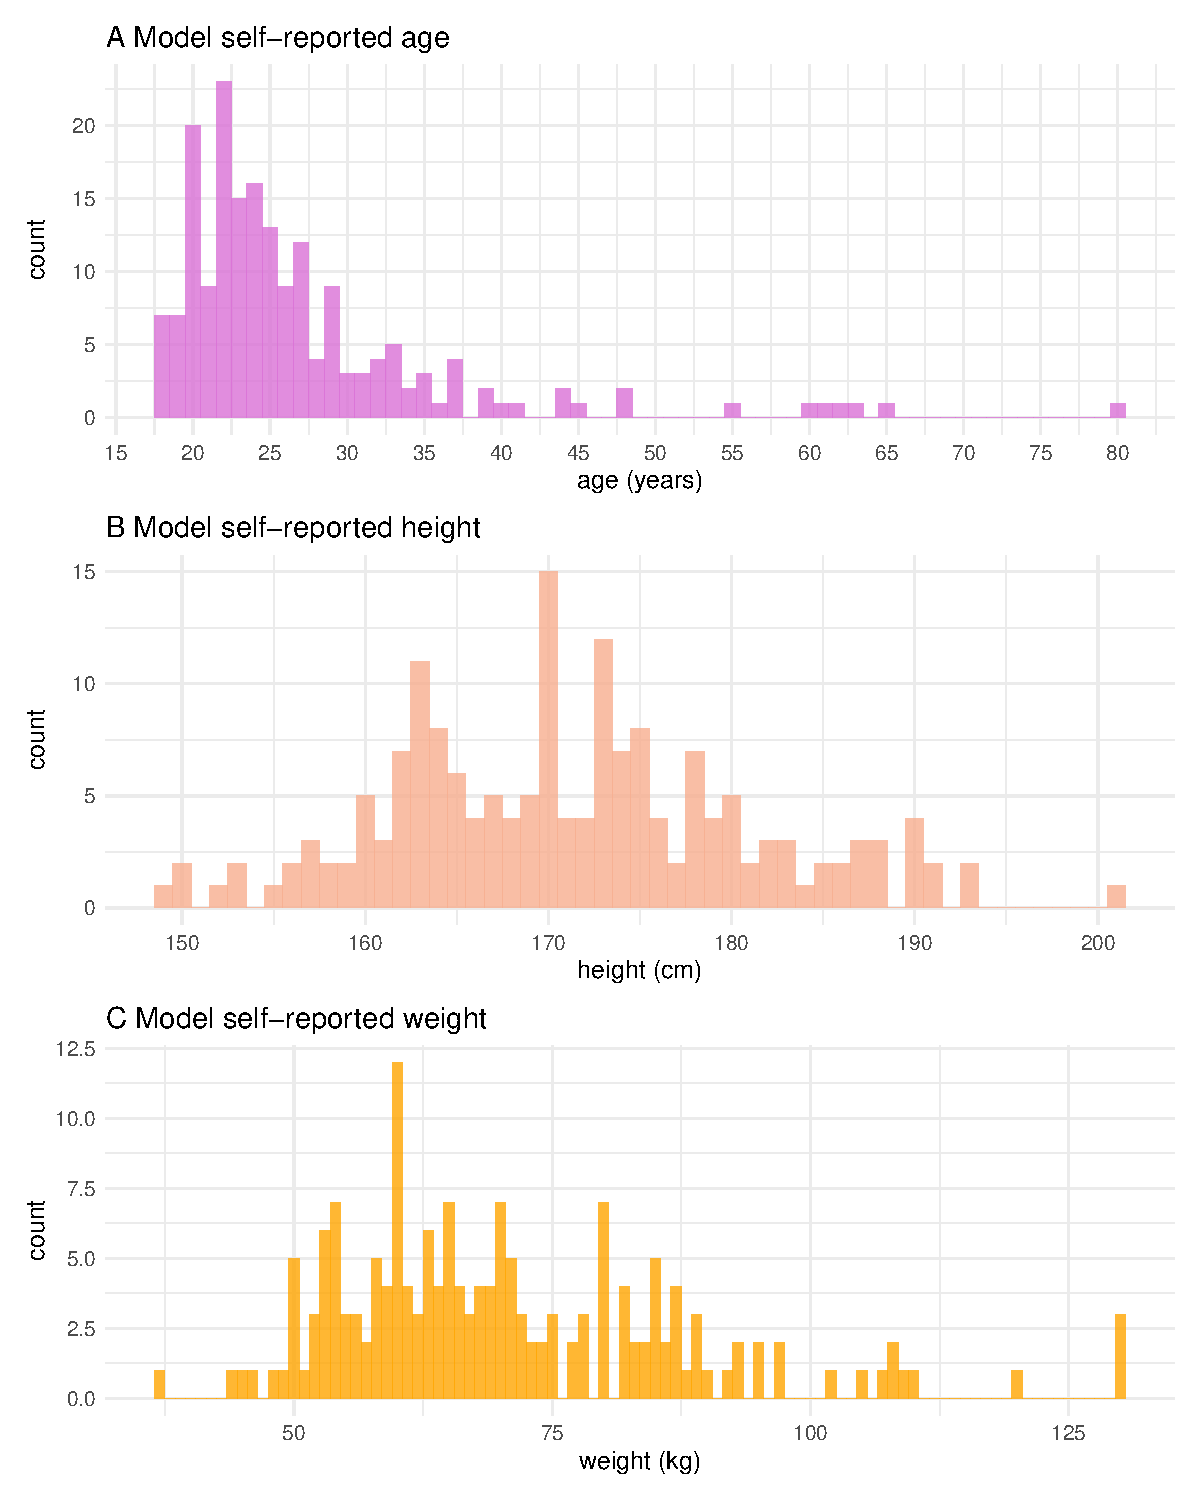
\includegraphics[keepaspectratio]{index_files/figure-pdf/fig-model-age-1.pdf}}

}

\end{figure}%

\textsubscript{Source:
\href{https://ManyFacesTeam.github.io/paper/index.qmd.html}{Article
Notebook}}

\begin{figure}[H]

\caption{\label{fig-rt-distribution}Median reaction time distribution in
Phase 2}

\centering{

\centering{

\pandocbounded{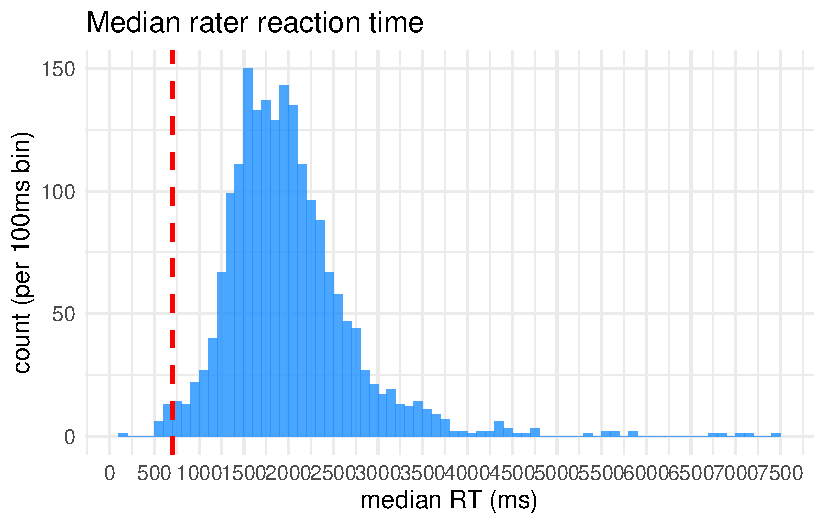
\includegraphics[keepaspectratio]{index_files/figure-pdf/fig-rt-distribution-1.pdf}}

}

\subcaption{\label{fig-rt-distribution}Note. Red dashed line indicates
exclusion cutoff.}

}

\end{figure}%

\textsubscript{Source:
\href{https://ManyFacesTeam.github.io/paper/index.qmd.html}{Article
Notebook}}

\protect\phantomsection\label{cell-fig-age}
\begin{figure}[H]

\caption{\label{fig-age}Histogram of rater age in Phase 2}

\centering{

\pandocbounded{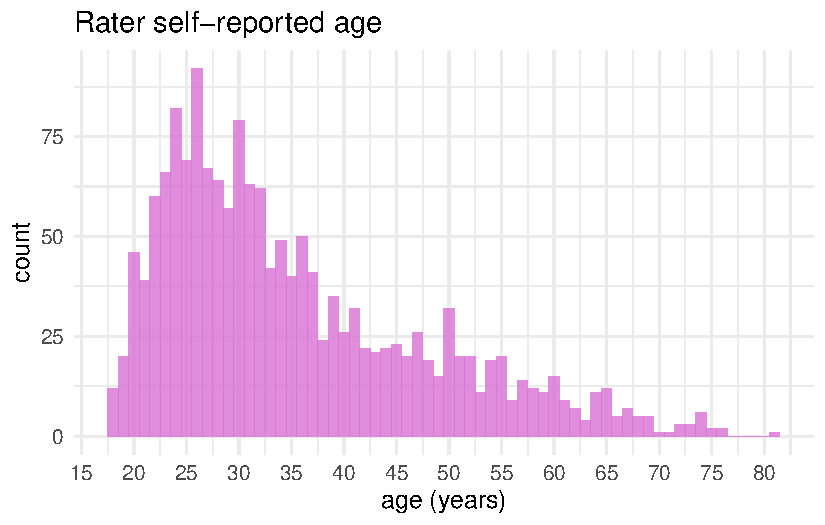
\includegraphics[keepaspectratio]{index_files/figure-pdf/fig-age-1.pdf}}

}

\end{figure}%

\textsubscript{Source:
\href{https://ManyFacesTeam.github.io/paper/index.qmd.html}{Article
Notebook}}

\global\setlength{\Oldarrayrulewidth}{\arrayrulewidth}

\global\setlength{\Oldtabcolsep}{\tabcolsep}

\setlength{\tabcolsep}{2pt}

\renewcommand*{\arraystretch}{1.5}



\providecommand{\ascline}[3]{\noalign{\global\arrayrulewidth #1}\arrayrulecolor[HTML]{#2}\cline{#3}}

\begin{longtable}[c]{|p{2.00in}|p{0.75in}}

\caption{\label{tbl-exclusions}The number of raters excluded from
analysis in Phase 2}

\tabularnewline

\ascline{1.5pt}{666666}{1-2}

\multicolumn{1}{>{\raggedright}m{\dimexpr 2in+0\tabcolsep}}{\textcolor[HTML]{000000}{\fontsize{11}{11}\selectfont{\global\setmainfont{Helvetica}{Reason\ for\ exclusion}}}} & \multicolumn{1}{>{\raggedleft}m{\dimexpr 0.75in+0\tabcolsep}}{\textcolor[HTML]{000000}{\fontsize{11}{11}\selectfont{\global\setmainfont{Helvetica}{N}}}} \\

\ascline{1.5pt}{666666}{1-2}\endfirsthead 

\ascline{1.5pt}{666666}{1-2}

\multicolumn{1}{>{\raggedright}m{\dimexpr 2in+0\tabcolsep}}{\textcolor[HTML]{000000}{\fontsize{11}{11}\selectfont{\global\setmainfont{Helvetica}{Reason\ for\ exclusion}}}} & \multicolumn{1}{>{\raggedleft}m{\dimexpr 0.75in+0\tabcolsep}}{\textcolor[HTML]{000000}{\fontsize{11}{11}\selectfont{\global\setmainfont{Helvetica}{N}}}} \\

\ascline{1.5pt}{666666}{1-2}\endhead



\multicolumn{1}{>{\raggedright}m{\dimexpr 2in+0\tabcolsep}}{\textcolor[HTML]{000000}{\fontsize{11}{11}\selectfont{\global\setmainfont{Helvetica}{Overly\ consistent}}}} & \multicolumn{1}{>{\raggedleft}m{\dimexpr 0.75in+0\tabcolsep}}{\textcolor[HTML]{000000}{\fontsize{11}{11}\selectfont{\global\setmainfont{Helvetica}{13}}}} \\





\multicolumn{1}{>{\raggedright}m{\dimexpr 2in+0\tabcolsep}}{\textcolor[HTML]{000000}{\fontsize{11}{11}\selectfont{\global\setmainfont{Helvetica}{Overly\ fast}}}} & \multicolumn{1}{>{\raggedleft}m{\dimexpr 0.75in+0\tabcolsep}}{\textcolor[HTML]{000000}{\fontsize{11}{11}\selectfont{\global\setmainfont{Helvetica}{20}}}} \\





\multicolumn{1}{>{\raggedright}m{\dimexpr 2in+0\tabcolsep}}{\textcolor[HTML]{000000}{\fontsize{11}{11}\selectfont{\global\setmainfont{Helvetica}{Failed\ honesty\ check}}}} & \multicolumn{1}{>{\raggedleft}m{\dimexpr 0.75in+0\tabcolsep}}{\textcolor[HTML]{000000}{\fontsize{11}{11}\selectfont{\global\setmainfont{Helvetica}{2}}}} \\





\multicolumn{1}{>{\raggedright}m{\dimexpr 2in+0\tabcolsep}}{\textcolor[HTML]{000000}{\fontsize{11}{11}\selectfont{\global\setmainfont{Helvetica}{Failed\ attention\ checks}}}} & \multicolumn{1}{>{\raggedleft}m{\dimexpr 0.75in+0\tabcolsep}}{\textcolor[HTML]{000000}{\fontsize{11}{11}\selectfont{\global\setmainfont{Helvetica}{19}}}} \\





\multicolumn{1}{>{\raggedright}m{\dimexpr 2in+0\tabcolsep}}{\textcolor[HTML]{000000}{\fontsize{11}{11}\selectfont{\global\setmainfont{Helvetica}{Total}}}} & \multicolumn{1}{>{\raggedleft}m{\dimexpr 0.75in+0\tabcolsep}}{\textcolor[HTML]{000000}{\fontsize{11}{11}\selectfont{\global\setmainfont{Helvetica}{49}}}} \\

\ascline{1.5pt}{666666}{1-2}


\end{longtable}

\arrayrulecolor[HTML]{000000}

\global\setlength{\arrayrulewidth}{\Oldarrayrulewidth}

\global\setlength{\tabcolsep}{\Oldtabcolsep}

\renewcommand*{\arraystretch}{1}

\textsubscript{Source:
\href{https://ManyFacesTeam.github.io/paper/index.qmd.html}{Article
Notebook}}

\emph{Note.} Multiple raters met more than one exclusion criterion;
therefore, the counts for individual criteria do not sum to the total
number of raters excluded.

\global\setlength{\Oldarrayrulewidth}{\arrayrulewidth}

\global\setlength{\Oldtabcolsep}{\tabcolsep}

\setlength{\tabcolsep}{2pt}

\renewcommand*{\arraystretch}{1.5}



\providecommand{\ascline}[3]{\noalign{\global\arrayrulewidth #1}\arrayrulecolor[HTML]{#2}\cline{#3}}

\begin{longtable}[c]{|p{2.00in}|p{0.75in}}

\caption{\label{tbl-raters-per-task}Number of raters per task in Phase
2}

\tabularnewline

\ascline{1.5pt}{666666}{1-2}

\multicolumn{1}{>{\raggedright}m{\dimexpr 2in+0\tabcolsep}}{\textcolor[HTML]{000000}{\fontsize{11}{11}\selectfont{\global\setmainfont{Helvetica}{Rating\ task}}}} & \multicolumn{1}{>{\raggedleft}m{\dimexpr 0.75in+0\tabcolsep}}{\textcolor[HTML]{000000}{\fontsize{11}{11}\selectfont{\global\setmainfont{Helvetica}{N}}}} \\

\ascline{1.5pt}{666666}{1-2}\endfirsthead 

\ascline{1.5pt}{666666}{1-2}

\multicolumn{1}{>{\raggedright}m{\dimexpr 2in+0\tabcolsep}}{\textcolor[HTML]{000000}{\fontsize{11}{11}\selectfont{\global\setmainfont{Helvetica}{Rating\ task}}}} & \multicolumn{1}{>{\raggedleft}m{\dimexpr 0.75in+0\tabcolsep}}{\textcolor[HTML]{000000}{\fontsize{11}{11}\selectfont{\global\setmainfont{Helvetica}{N}}}} \\

\ascline{1.5pt}{666666}{1-2}\endhead



\multicolumn{1}{>{\raggedright}m{\dimexpr 2in+0\tabcolsep}}{\textcolor[HTML]{000000}{\fontsize{11}{11}\selectfont{\global\setmainfont{Helvetica}{age}}}} & \multicolumn{1}{>{\raggedleft}m{\dimexpr 0.75in+0\tabcolsep}}{\textcolor[HTML]{000000}{\fontsize{11}{11}\selectfont{\global\setmainfont{Helvetica}{85}}}} \\





\multicolumn{1}{>{\raggedright}m{\dimexpr 2in+0\tabcolsep}}{\textcolor[HTML]{000000}{\fontsize{11}{11}\selectfont{\global\setmainfont{Helvetica}{anger\ intensity}}}} & \multicolumn{1}{>{\raggedleft}m{\dimexpr 0.75in+0\tabcolsep}}{\textcolor[HTML]{000000}{\fontsize{11}{11}\selectfont{\global\setmainfont{Helvetica}{84}}}} \\





\multicolumn{1}{>{\raggedright}m{\dimexpr 2in+0\tabcolsep}}{\textcolor[HTML]{000000}{\fontsize{11}{11}\selectfont{\global\setmainfont{Helvetica}{attractive}}}} & \multicolumn{1}{>{\raggedleft}m{\dimexpr 0.75in+0\tabcolsep}}{\textcolor[HTML]{000000}{\fontsize{11}{11}\selectfont{\global\setmainfont{Helvetica}{84}}}} \\





\multicolumn{1}{>{\raggedright}m{\dimexpr 2in+0\tabcolsep}}{\textcolor[HTML]{000000}{\fontsize{11}{11}\selectfont{\global\setmainfont{Helvetica}{attractive\ (unstandardized)}}}} & \multicolumn{1}{>{\raggedleft}m{\dimexpr 0.75in+0\tabcolsep}}{\textcolor[HTML]{000000}{\fontsize{11}{11}\selectfont{\global\setmainfont{Helvetica}{84}}}} \\





\multicolumn{1}{>{\raggedright}m{\dimexpr 2in+0\tabcolsep}}{\textcolor[HTML]{000000}{\fontsize{11}{11}\selectfont{\global\setmainfont{Helvetica}{disgust\ intensity}}}} & \multicolumn{1}{>{\raggedleft}m{\dimexpr 0.75in+0\tabcolsep}}{\textcolor[HTML]{000000}{\fontsize{11}{11}\selectfont{\global\setmainfont{Helvetica}{91}}}} \\





\multicolumn{1}{>{\raggedright}m{\dimexpr 2in+0\tabcolsep}}{\textcolor[HTML]{000000}{\fontsize{11}{11}\selectfont{\global\setmainfont{Helvetica}{dominant}}}} & \multicolumn{1}{>{\raggedleft}m{\dimexpr 0.75in+0\tabcolsep}}{\textcolor[HTML]{000000}{\fontsize{11}{11}\selectfont{\global\setmainfont{Helvetica}{91}}}} \\





\multicolumn{1}{>{\raggedright}m{\dimexpr 2in+0\tabcolsep}}{\textcolor[HTML]{000000}{\fontsize{11}{11}\selectfont{\global\setmainfont{Helvetica}{dominant\ (unstandardized)}}}} & \multicolumn{1}{>{\raggedleft}m{\dimexpr 0.75in+0\tabcolsep}}{\textcolor[HTML]{000000}{\fontsize{11}{11}\selectfont{\global\setmainfont{Helvetica}{94}}}} \\





\multicolumn{1}{>{\raggedright}m{\dimexpr 2in+0\tabcolsep}}{\textcolor[HTML]{000000}{\fontsize{11}{11}\selectfont{\global\setmainfont{Helvetica}{emotion\ categorization\ 1}}}} & \multicolumn{1}{>{\raggedleft}m{\dimexpr 0.75in+0\tabcolsep}}{\textcolor[HTML]{000000}{\fontsize{11}{11}\selectfont{\global\setmainfont{Helvetica}{97}}}} \\





\multicolumn{1}{>{\raggedright}m{\dimexpr 2in+0\tabcolsep}}{\textcolor[HTML]{000000}{\fontsize{11}{11}\selectfont{\global\setmainfont{Helvetica}{emotion\ categorization\ 2}}}} & \multicolumn{1}{>{\raggedleft}m{\dimexpr 0.75in+0\tabcolsep}}{\textcolor[HTML]{000000}{\fontsize{11}{11}\selectfont{\global\setmainfont{Helvetica}{87}}}} \\





\multicolumn{1}{>{\raggedright}m{\dimexpr 2in+0\tabcolsep}}{\textcolor[HTML]{000000}{\fontsize{11}{11}\selectfont{\global\setmainfont{Helvetica}{emotion\ categorization\ 3}}}} & \multicolumn{1}{>{\raggedleft}m{\dimexpr 0.75in+0\tabcolsep}}{\textcolor[HTML]{000000}{\fontsize{11}{11}\selectfont{\global\setmainfont{Helvetica}{88}}}} \\





\multicolumn{1}{>{\raggedright}m{\dimexpr 2in+0\tabcolsep}}{\textcolor[HTML]{000000}{\fontsize{11}{11}\selectfont{\global\setmainfont{Helvetica}{emotion\ categorization\ 4}}}} & \multicolumn{1}{>{\raggedleft}m{\dimexpr 0.75in+0\tabcolsep}}{\textcolor[HTML]{000000}{\fontsize{11}{11}\selectfont{\global\setmainfont{Helvetica}{97}}}} \\





\multicolumn{1}{>{\raggedright}m{\dimexpr 2in+0\tabcolsep}}{\textcolor[HTML]{000000}{\fontsize{11}{11}\selectfont{\global\setmainfont{Helvetica}{emotion\ categorization\ 5}}}} & \multicolumn{1}{>{\raggedleft}m{\dimexpr 0.75in+0\tabcolsep}}{\textcolor[HTML]{000000}{\fontsize{11}{11}\selectfont{\global\setmainfont{Helvetica}{86}}}} \\





\multicolumn{1}{>{\raggedright}m{\dimexpr 2in+0\tabcolsep}}{\textcolor[HTML]{000000}{\fontsize{11}{11}\selectfont{\global\setmainfont{Helvetica}{emotion\ categorization\ 6}}}} & \multicolumn{1}{>{\raggedleft}m{\dimexpr 0.75in+0\tabcolsep}}{\textcolor[HTML]{000000}{\fontsize{11}{11}\selectfont{\global\setmainfont{Helvetica}{114}}}} \\





\multicolumn{1}{>{\raggedright}m{\dimexpr 2in+0\tabcolsep}}{\textcolor[HTML]{000000}{\fontsize{11}{11}\selectfont{\global\setmainfont{Helvetica}{fear\ intensity}}}} & \multicolumn{1}{>{\raggedleft}m{\dimexpr 0.75in+0\tabcolsep}}{\textcolor[HTML]{000000}{\fontsize{11}{11}\selectfont{\global\setmainfont{Helvetica}{90}}}} \\





\multicolumn{1}{>{\raggedright}m{\dimexpr 2in+0\tabcolsep}}{\textcolor[HTML]{000000}{\fontsize{11}{11}\selectfont{\global\setmainfont{Helvetica}{gender-typical}}}} & \multicolumn{1}{>{\raggedleft}m{\dimexpr 0.75in+0\tabcolsep}}{\textcolor[HTML]{000000}{\fontsize{11}{11}\selectfont{\global\setmainfont{Helvetica}{80}}}} \\





\multicolumn{1}{>{\raggedright}m{\dimexpr 2in+0\tabcolsep}}{\textcolor[HTML]{000000}{\fontsize{11}{11}\selectfont{\global\setmainfont{Helvetica}{happiness\ intensity}}}} & \multicolumn{1}{>{\raggedleft}m{\dimexpr 0.75in+0\tabcolsep}}{\textcolor[HTML]{000000}{\fontsize{11}{11}\selectfont{\global\setmainfont{Helvetica}{91}}}} \\





\multicolumn{1}{>{\raggedright}m{\dimexpr 2in+0\tabcolsep}}{\textcolor[HTML]{000000}{\fontsize{11}{11}\selectfont{\global\setmainfont{Helvetica}{memorable}}}} & \multicolumn{1}{>{\raggedleft}m{\dimexpr 0.75in+0\tabcolsep}}{\textcolor[HTML]{000000}{\fontsize{11}{11}\selectfont{\global\setmainfont{Helvetica}{82}}}} \\





\multicolumn{1}{>{\raggedright}m{\dimexpr 2in+0\tabcolsep}}{\textcolor[HTML]{000000}{\fontsize{11}{11}\selectfont{\global\setmainfont{Helvetica}{sadness\ intensity}}}} & \multicolumn{1}{>{\raggedleft}m{\dimexpr 0.75in+0\tabcolsep}}{\textcolor[HTML]{000000}{\fontsize{11}{11}\selectfont{\global\setmainfont{Helvetica}{103}}}} \\





\multicolumn{1}{>{\raggedright}m{\dimexpr 2in+0\tabcolsep}}{\textcolor[HTML]{000000}{\fontsize{11}{11}\selectfont{\global\setmainfont{Helvetica}{surprise\ intensity}}}} & \multicolumn{1}{>{\raggedleft}m{\dimexpr 0.75in+0\tabcolsep}}{\textcolor[HTML]{000000}{\fontsize{11}{11}\selectfont{\global\setmainfont{Helvetica}{84}}}} \\





\multicolumn{1}{>{\raggedright}m{\dimexpr 2in+0\tabcolsep}}{\textcolor[HTML]{000000}{\fontsize{11}{11}\selectfont{\global\setmainfont{Helvetica}{trustworthy}}}} & \multicolumn{1}{>{\raggedleft}m{\dimexpr 0.75in+0\tabcolsep}}{\textcolor[HTML]{000000}{\fontsize{11}{11}\selectfont{\global\setmainfont{Helvetica}{88}}}} \\





\multicolumn{1}{>{\raggedright}m{\dimexpr 2in+0\tabcolsep}}{\textcolor[HTML]{000000}{\fontsize{11}{11}\selectfont{\global\setmainfont{Helvetica}{trustworthy\ (unstandardized)}}}} & \multicolumn{1}{>{\raggedleft}m{\dimexpr 0.75in+0\tabcolsep}}{\textcolor[HTML]{000000}{\fontsize{11}{11}\selectfont{\global\setmainfont{Helvetica}{87}}}} \\

\ascline{1.5pt}{666666}{1-2}


\end{longtable}

\arrayrulecolor[HTML]{000000}

\global\setlength{\arrayrulewidth}{\Oldarrayrulewidth}

\global\setlength{\tabcolsep}{\Oldtabcolsep}

\renewcommand*{\arraystretch}{1}

\textsubscript{Source:
\href{https://ManyFacesTeam.github.io/paper/index.qmd.html}{Article
Notebook}}

\emph{Note}. The emotion categorization task was broken into 6
counterbalanced versions.

\global\setlength{\Oldarrayrulewidth}{\arrayrulewidth}

\global\setlength{\Oldtabcolsep}{\tabcolsep}

\setlength{\tabcolsep}{2pt}

\renewcommand*{\arraystretch}{1.5}



\providecommand{\ascline}[3]{\noalign{\global\arrayrulewidth #1}\arrayrulecolor[HTML]{#2}\cline{#3}}

\begin{longtable}[c]{|p{2.00in}|p{0.75in}}

\caption{\label{tbl-raters-country}Rater country of residence in Phase
2}

\tabularnewline

\ascline{1.5pt}{666666}{1-2}

\multicolumn{1}{>{\raggedright}m{\dimexpr 2in+0\tabcolsep}}{\textcolor[HTML]{000000}{\fontsize{11}{11}\selectfont{\global\setmainfont{Helvetica}{Country\ of\ residence}}}} & \multicolumn{1}{>{\raggedleft}m{\dimexpr 0.75in+0\tabcolsep}}{\textcolor[HTML]{000000}{\fontsize{11}{11}\selectfont{\global\setmainfont{Helvetica}{N}}}} \\

\ascline{1.5pt}{666666}{1-2}\endfirsthead 

\ascline{1.5pt}{666666}{1-2}

\multicolumn{1}{>{\raggedright}m{\dimexpr 2in+0\tabcolsep}}{\textcolor[HTML]{000000}{\fontsize{11}{11}\selectfont{\global\setmainfont{Helvetica}{Country\ of\ residence}}}} & \multicolumn{1}{>{\raggedleft}m{\dimexpr 0.75in+0\tabcolsep}}{\textcolor[HTML]{000000}{\fontsize{11}{11}\selectfont{\global\setmainfont{Helvetica}{N}}}} \\

\ascline{1.5pt}{666666}{1-2}\endhead



\multicolumn{1}{>{\raggedright}m{\dimexpr 2in+0\tabcolsep}}{\textcolor[HTML]{000000}{\fontsize{11}{11}\selectfont{\global\setmainfont{Helvetica}{South\ Africa}}}} & \multicolumn{1}{>{\raggedleft}m{\dimexpr 0.75in+0\tabcolsep}}{\textcolor[HTML]{000000}{\fontsize{11}{11}\selectfont{\global\setmainfont{Helvetica}{814}}}} \\





\multicolumn{1}{>{\raggedright}m{\dimexpr 2in+0\tabcolsep}}{\textcolor[HTML]{000000}{\fontsize{11}{11}\selectfont{\global\setmainfont{Helvetica}{United\ Kingdom}}}} & \multicolumn{1}{>{\raggedleft}m{\dimexpr 0.75in+0\tabcolsep}}{\textcolor[HTML]{000000}{\fontsize{11}{11}\selectfont{\global\setmainfont{Helvetica}{253}}}} \\





\multicolumn{1}{>{\raggedright}m{\dimexpr 2in+0\tabcolsep}}{\textcolor[HTML]{000000}{\fontsize{11}{11}\selectfont{\global\setmainfont{Helvetica}{United\ States}}}} & \multicolumn{1}{>{\raggedleft}m{\dimexpr 0.75in+0\tabcolsep}}{\textcolor[HTML]{000000}{\fontsize{11}{11}\selectfont{\global\setmainfont{Helvetica}{219}}}} \\





\multicolumn{1}{>{\raggedright}m{\dimexpr 2in+0\tabcolsep}}{\textcolor[HTML]{000000}{\fontsize{11}{11}\selectfont{\global\setmainfont{Helvetica}{Poland}}}} & \multicolumn{1}{>{\raggedleft}m{\dimexpr 0.75in+0\tabcolsep}}{\textcolor[HTML]{000000}{\fontsize{11}{11}\selectfont{\global\setmainfont{Helvetica}{49}}}} \\





\multicolumn{1}{>{\raggedright}m{\dimexpr 2in+0\tabcolsep}}{\textcolor[HTML]{000000}{\fontsize{11}{11}\selectfont{\global\setmainfont{Helvetica}{Portugal}}}} & \multicolumn{1}{>{\raggedleft}m{\dimexpr 0.75in+0\tabcolsep}}{\textcolor[HTML]{000000}{\fontsize{11}{11}\selectfont{\global\setmainfont{Helvetica}{44}}}} \\





\multicolumn{1}{>{\raggedright}m{\dimexpr 2in+0\tabcolsep}}{\textcolor[HTML]{000000}{\fontsize{11}{11}\selectfont{\global\setmainfont{Helvetica}{Canada}}}} & \multicolumn{1}{>{\raggedleft}m{\dimexpr 0.75in+0\tabcolsep}}{\textcolor[HTML]{000000}{\fontsize{11}{11}\selectfont{\global\setmainfont{Helvetica}{41}}}} \\





\multicolumn{1}{>{\raggedright}m{\dimexpr 2in+0\tabcolsep}}{\textcolor[HTML]{000000}{\fontsize{11}{11}\selectfont{\global\setmainfont{Helvetica}{Spain}}}} & \multicolumn{1}{>{\raggedleft}m{\dimexpr 0.75in+0\tabcolsep}}{\textcolor[HTML]{000000}{\fontsize{11}{11}\selectfont{\global\setmainfont{Helvetica}{34}}}} \\





\multicolumn{1}{>{\raggedright}m{\dimexpr 2in+0\tabcolsep}}{\textcolor[HTML]{000000}{\fontsize{11}{11}\selectfont{\global\setmainfont{Helvetica}{Italy}}}} & \multicolumn{1}{>{\raggedleft}m{\dimexpr 0.75in+0\tabcolsep}}{\textcolor[HTML]{000000}{\fontsize{11}{11}\selectfont{\global\setmainfont{Helvetica}{27}}}} \\





\multicolumn{1}{>{\raggedright}m{\dimexpr 2in+0\tabcolsep}}{\textcolor[HTML]{000000}{\fontsize{11}{11}\selectfont{\global\setmainfont{Helvetica}{Kenya}}}} & \multicolumn{1}{>{\raggedleft}m{\dimexpr 0.75in+0\tabcolsep}}{\textcolor[HTML]{000000}{\fontsize{11}{11}\selectfont{\global\setmainfont{Helvetica}{26}}}} \\





\multicolumn{1}{>{\raggedright}m{\dimexpr 2in+0\tabcolsep}}{\textcolor[HTML]{000000}{\fontsize{11}{11}\selectfont{\global\setmainfont{Helvetica}{Germany}}}} & \multicolumn{1}{>{\raggedleft}m{\dimexpr 0.75in+0\tabcolsep}}{\textcolor[HTML]{000000}{\fontsize{11}{11}\selectfont{\global\setmainfont{Helvetica}{18}}}} \\





\multicolumn{1}{>{\raggedright}m{\dimexpr 2in+0\tabcolsep}}{\textcolor[HTML]{000000}{\fontsize{11}{11}\selectfont{\global\setmainfont{Helvetica}{Greece}}}} & \multicolumn{1}{>{\raggedleft}m{\dimexpr 0.75in+0\tabcolsep}}{\textcolor[HTML]{000000}{\fontsize{11}{11}\selectfont{\global\setmainfont{Helvetica}{17}}}} \\





\multicolumn{1}{>{\raggedright}m{\dimexpr 2in+0\tabcolsep}}{\textcolor[HTML]{000000}{\fontsize{11}{11}\selectfont{\global\setmainfont{Helvetica}{Hungary}}}} & \multicolumn{1}{>{\raggedleft}m{\dimexpr 0.75in+0\tabcolsep}}{\textcolor[HTML]{000000}{\fontsize{11}{11}\selectfont{\global\setmainfont{Helvetica}{13}}}} \\





\multicolumn{1}{>{\raggedright}m{\dimexpr 2in+0\tabcolsep}}{\textcolor[HTML]{000000}{\fontsize{11}{11}\selectfont{\global\setmainfont{Helvetica}{India,\ Mexico}}}} & \multicolumn{1}{>{\raggedleft}m{\dimexpr 0.75in+0\tabcolsep}}{\textcolor[HTML]{000000}{\fontsize{11}{11}\selectfont{\global\setmainfont{Helvetica}{11}}}} \\





\multicolumn{1}{>{\raggedright}m{\dimexpr 2in+0\tabcolsep}}{\textcolor[HTML]{000000}{\fontsize{11}{11}\selectfont{\global\setmainfont{Helvetica}{Chile}}}} & \multicolumn{1}{>{\raggedleft}m{\dimexpr 0.75in+0\tabcolsep}}{\textcolor[HTML]{000000}{\fontsize{11}{11}\selectfont{\global\setmainfont{Helvetica}{10}}}} \\





\multicolumn{1}{>{\raggedright}m{\dimexpr 2in+0\tabcolsep}}{\textcolor[HTML]{000000}{\fontsize{11}{11}\selectfont{\global\setmainfont{Helvetica}{France}}}} & \multicolumn{1}{>{\raggedleft}m{\dimexpr 0.75in+0\tabcolsep}}{\textcolor[HTML]{000000}{\fontsize{11}{11}\selectfont{\global\setmainfont{Helvetica}{9}}}} \\





\multicolumn{1}{>{\raggedright}m{\dimexpr 2in+0\tabcolsep}}{\textcolor[HTML]{000000}{\fontsize{11}{11}\selectfont{\global\setmainfont{Helvetica}{Ireland}}}} & \multicolumn{1}{>{\raggedleft}m{\dimexpr 0.75in+0\tabcolsep}}{\textcolor[HTML]{000000}{\fontsize{11}{11}\selectfont{\global\setmainfont{Helvetica}{6}}}} \\





\multicolumn{1}{>{\raggedright}m{\dimexpr 2in+0\tabcolsep}}{\textcolor[HTML]{000000}{\fontsize{11}{11}\selectfont{\global\setmainfont{Helvetica}{Brazil,\ Netherlands,\ Sweden}}}} & \multicolumn{1}{>{\raggedleft}m{\dimexpr 0.75in+0\tabcolsep}}{\textcolor[HTML]{000000}{\fontsize{11}{11}\selectfont{\global\setmainfont{Helvetica}{5}}}} \\





\multicolumn{1}{>{\raggedright}m{\dimexpr 2in+0\tabcolsep}}{\textcolor[HTML]{000000}{\fontsize{11}{11}\selectfont{\global\setmainfont{Helvetica}{Australia,\ Croatia}}}} & \multicolumn{1}{>{\raggedleft}m{\dimexpr 0.75in+0\tabcolsep}}{\textcolor[HTML]{000000}{\fontsize{11}{11}\selectfont{\global\setmainfont{Helvetica}{4}}}} \\





\multicolumn{1}{>{\raggedright}m{\dimexpr 2in+0\tabcolsep}}{\textcolor[HTML]{000000}{\fontsize{11}{11}\selectfont{\global\setmainfont{Helvetica}{Czechia,\ Estonia,\ Latvia}}}} & \multicolumn{1}{>{\raggedleft}m{\dimexpr 0.75in+0\tabcolsep}}{\textcolor[HTML]{000000}{\fontsize{11}{11}\selectfont{\global\setmainfont{Helvetica}{3}}}} \\





\multicolumn{1}{>{\raggedright}m{\dimexpr 2in+0\tabcolsep}}{\textcolor[HTML]{000000}{\fontsize{11}{11}\selectfont{\global\setmainfont{Helvetica}{Belgium,\ Denmark,\ Israel,\ Slovenia,\ Switzerland}}}} & \multicolumn{1}{>{\raggedleft}m{\dimexpr 0.75in+0\tabcolsep}}{\textcolor[HTML]{000000}{\fontsize{11}{11}\selectfont{\global\setmainfont{Helvetica}{2}}}} \\





\multicolumn{1}{>{\raggedright}m{\dimexpr 2in+0\tabcolsep}}{\textcolor[HTML]{000000}{\fontsize{11}{11}\selectfont{\global\setmainfont{Helvetica}{Algeria,\ Argentina,\ Austria,\ China,\ Finland,\ Kazakhstan,\ Morocco,\ Slovakia}}}} & \multicolumn{1}{>{\raggedleft}m{\dimexpr 0.75in+0\tabcolsep}}{\textcolor[HTML]{000000}{\fontsize{11}{11}\selectfont{\global\setmainfont{Helvetica}{1}}}} \\

\ascline{1.5pt}{666666}{1-2}


\end{longtable}

\arrayrulecolor[HTML]{000000}

\global\setlength{\arrayrulewidth}{\Oldarrayrulewidth}

\global\setlength{\tabcolsep}{\Oldtabcolsep}

\renewcommand*{\arraystretch}{1}

\textsubscript{Source:
\href{https://ManyFacesTeam.github.io/paper/index.qmd.html}{Article
Notebook}}

\emph{Note}. Where rows list more than one country, \emph{each} country
in that row has the specified number of participants.

\global\setlength{\Oldarrayrulewidth}{\arrayrulewidth}

\global\setlength{\Oldtabcolsep}{\tabcolsep}

\setlength{\tabcolsep}{2pt}

\renewcommand*{\arraystretch}{1.5}



\providecommand{\ascline}[3]{\noalign{\global\arrayrulewidth #1}\arrayrulecolor[HTML]{#2}\cline{#3}}

\begin{longtable}[c]{|p{1.50in}|p{0.20in}|p{0.50in}|p{1.00in}|p{0.50in}|p{0.50in}}

\caption{\label{tbl-icc}Intraclass correlation coefficients, Cronbach's
alpha, and McDonald's omega for trait and emotion intensity ratings}

\tabularnewline

\ascline{1.5pt}{666666}{1-6}

\multicolumn{1}{>{\raggedright}m{\dimexpr 1.5in+0\tabcolsep}}{\textcolor[HTML]{000000}{\fontsize{11}{11}\selectfont{\global\setmainfont{Helvetica}{Rating}}}} & \multicolumn{1}{>{\raggedleft}m{\dimexpr 0.2in+0\tabcolsep}}{\textcolor[HTML]{000000}{\fontsize{11}{11}\selectfont{\global\setmainfont{Helvetica}{N}}}} & \multicolumn{1}{>{\raggedleft}m{\dimexpr 0.5in+0\tabcolsep}}{\textcolor[HTML]{000000}{\fontsize{11}{11}\selectfont{\global\setmainfont{Helvetica}{ICC}}}} & \multicolumn{1}{>{\raggedright}m{\dimexpr 1in+0\tabcolsep}}{\textcolor[HTML]{000000}{\fontsize{11}{11}\selectfont{\global\setmainfont{Helvetica}{[95\%\ CI]}}}} & \multicolumn{1}{>{\raggedleft}m{\dimexpr 0.5in+0\tabcolsep}}{\textcolor[HTML]{000000}{\fontsize{11}{11}\selectfont{\global\setmainfont{Helvetica}{alpha}}}} & \multicolumn{1}{>{\raggedleft}m{\dimexpr 0.5in+0\tabcolsep}}{\textcolor[HTML]{000000}{\fontsize{11}{11}\selectfont{\global\setmainfont{Helvetica}{omega}}}} \\

\ascline{1.5pt}{666666}{1-6}\endfirsthead 

\ascline{1.5pt}{666666}{1-6}

\multicolumn{1}{>{\raggedright}m{\dimexpr 1.5in+0\tabcolsep}}{\textcolor[HTML]{000000}{\fontsize{11}{11}\selectfont{\global\setmainfont{Helvetica}{Rating}}}} & \multicolumn{1}{>{\raggedleft}m{\dimexpr 0.2in+0\tabcolsep}}{\textcolor[HTML]{000000}{\fontsize{11}{11}\selectfont{\global\setmainfont{Helvetica}{N}}}} & \multicolumn{1}{>{\raggedleft}m{\dimexpr 0.5in+0\tabcolsep}}{\textcolor[HTML]{000000}{\fontsize{11}{11}\selectfont{\global\setmainfont{Helvetica}{ICC}}}} & \multicolumn{1}{>{\raggedright}m{\dimexpr 1in+0\tabcolsep}}{\textcolor[HTML]{000000}{\fontsize{11}{11}\selectfont{\global\setmainfont{Helvetica}{[95\%\ CI]}}}} & \multicolumn{1}{>{\raggedleft}m{\dimexpr 0.5in+0\tabcolsep}}{\textcolor[HTML]{000000}{\fontsize{11}{11}\selectfont{\global\setmainfont{Helvetica}{alpha}}}} & \multicolumn{1}{>{\raggedleft}m{\dimexpr 0.5in+0\tabcolsep}}{\textcolor[HTML]{000000}{\fontsize{11}{11}\selectfont{\global\setmainfont{Helvetica}{omega}}}} \\

\ascline{1.5pt}{666666}{1-6}\endhead



\multicolumn{1}{>{\raggedright}m{\dimexpr 1.5in+0\tabcolsep}}{\textcolor[HTML]{000000}{\fontsize{11}{11}\selectfont{\global\setmainfont{Helvetica}{attractive}}}} & \multicolumn{1}{>{\raggedleft}m{\dimexpr 0.2in+0\tabcolsep}}{\textcolor[HTML]{000000}{\fontsize{11}{11}\selectfont{\global\setmainfont{Helvetica}{84}}}} & \multicolumn{1}{>{\raggedleft}m{\dimexpr 0.5in+0\tabcolsep}}{\textcolor[HTML]{000000}{\fontsize{11}{11}\selectfont{\global\setmainfont{Helvetica}{0.93}}}} & \multicolumn{1}{>{\raggedright}m{\dimexpr 1in+0\tabcolsep}}{\textcolor[HTML]{000000}{\fontsize{11}{11}\selectfont{\global\setmainfont{Helvetica}{[0.91,\ 0.95]}}}} & \multicolumn{1}{>{\raggedleft}m{\dimexpr 0.5in+0\tabcolsep}}{\textcolor[HTML]{000000}{\fontsize{11}{11}\selectfont{\global\setmainfont{Helvetica}{0.96}}}} & \multicolumn{1}{>{\raggedleft}m{\dimexpr 0.5in+0\tabcolsep}}{\textcolor[HTML]{000000}{\fontsize{11}{11}\selectfont{\global\setmainfont{Helvetica}{0.97}}}} \\





\multicolumn{1}{>{\raggedright}m{\dimexpr 1.5in+0\tabcolsep}}{\textcolor[HTML]{000000}{\fontsize{11}{11}\selectfont{\global\setmainfont{Helvetica}{dominant}}}} & \multicolumn{1}{>{\raggedleft}m{\dimexpr 0.2in+0\tabcolsep}}{\textcolor[HTML]{000000}{\fontsize{11}{11}\selectfont{\global\setmainfont{Helvetica}{91}}}} & \multicolumn{1}{>{\raggedleft}m{\dimexpr 0.5in+0\tabcolsep}}{\textcolor[HTML]{000000}{\fontsize{11}{11}\selectfont{\global\setmainfont{Helvetica}{0.88}}}} & \multicolumn{1}{>{\raggedright}m{\dimexpr 1in+0\tabcolsep}}{\textcolor[HTML]{000000}{\fontsize{11}{11}\selectfont{\global\setmainfont{Helvetica}{[0.85,\ 0.9]}}}} & \multicolumn{1}{>{\raggedleft}m{\dimexpr 0.5in+0\tabcolsep}}{\textcolor[HTML]{000000}{\fontsize{11}{11}\selectfont{\global\setmainfont{Helvetica}{0.91}}}} & \multicolumn{1}{>{\raggedleft}m{\dimexpr 0.5in+0\tabcolsep}}{\textcolor[HTML]{000000}{\fontsize{11}{11}\selectfont{\global\setmainfont{Helvetica}{0.92}}}} \\





\multicolumn{1}{>{\raggedright}m{\dimexpr 1.5in+0\tabcolsep}}{\textcolor[HTML]{000000}{\fontsize{11}{11}\selectfont{\global\setmainfont{Helvetica}{trustworthy}}}} & \multicolumn{1}{>{\raggedleft}m{\dimexpr 0.2in+0\tabcolsep}}{\textcolor[HTML]{000000}{\fontsize{11}{11}\selectfont{\global\setmainfont{Helvetica}{88}}}} & \multicolumn{1}{>{\raggedleft}m{\dimexpr 0.5in+0\tabcolsep}}{\textcolor[HTML]{000000}{\fontsize{11}{11}\selectfont{\global\setmainfont{Helvetica}{0.88}}}} & \multicolumn{1}{>{\raggedright}m{\dimexpr 1in+0\tabcolsep}}{\textcolor[HTML]{000000}{\fontsize{11}{11}\selectfont{\global\setmainfont{Helvetica}{[0.85,\ 0.9]}}}} & \multicolumn{1}{>{\raggedleft}m{\dimexpr 0.5in+0\tabcolsep}}{\textcolor[HTML]{000000}{\fontsize{11}{11}\selectfont{\global\setmainfont{Helvetica}{0.91}}}} & \multicolumn{1}{>{\raggedleft}m{\dimexpr 0.5in+0\tabcolsep}}{\textcolor[HTML]{000000}{\fontsize{11}{11}\selectfont{\global\setmainfont{Helvetica}{0.93}}}} \\





\multicolumn{1}{>{\raggedright}m{\dimexpr 1.5in+0\tabcolsep}}{\textcolor[HTML]{000000}{\fontsize{11}{11}\selectfont{\global\setmainfont{Helvetica}{gender-typical}}}} & \multicolumn{1}{>{\raggedleft}m{\dimexpr 0.2in+0\tabcolsep}}{\textcolor[HTML]{000000}{\fontsize{11}{11}\selectfont{\global\setmainfont{Helvetica}{80}}}} & \multicolumn{1}{>{\raggedleft}m{\dimexpr 0.5in+0\tabcolsep}}{\textcolor[HTML]{000000}{\fontsize{11}{11}\selectfont{\global\setmainfont{Helvetica}{0.87}}}} & \multicolumn{1}{>{\raggedright}m{\dimexpr 1in+0\tabcolsep}}{\textcolor[HTML]{000000}{\fontsize{11}{11}\selectfont{\global\setmainfont{Helvetica}{[0.84,\ 0.9]}}}} & \multicolumn{1}{>{\raggedleft}m{\dimexpr 0.5in+0\tabcolsep}}{\textcolor[HTML]{000000}{\fontsize{11}{11}\selectfont{\global\setmainfont{Helvetica}{0.92}}}} & \multicolumn{1}{>{\raggedleft}m{\dimexpr 0.5in+0\tabcolsep}}{\textcolor[HTML]{000000}{\fontsize{11}{11}\selectfont{\global\setmainfont{Helvetica}{0.93}}}} \\





\multicolumn{1}{>{\raggedright}m{\dimexpr 1.5in+0\tabcolsep}}{\textcolor[HTML]{000000}{\fontsize{11}{11}\selectfont{\global\setmainfont{Helvetica}{memorable}}}} & \multicolumn{1}{>{\raggedleft}m{\dimexpr 0.2in+0\tabcolsep}}{\textcolor[HTML]{000000}{\fontsize{11}{11}\selectfont{\global\setmainfont{Helvetica}{82}}}} & \multicolumn{1}{>{\raggedleft}m{\dimexpr 0.5in+0\tabcolsep}}{\textcolor[HTML]{000000}{\fontsize{11}{11}\selectfont{\global\setmainfont{Helvetica}{0.60}}}} & \multicolumn{1}{>{\raggedright}m{\dimexpr 1in+0\tabcolsep}}{\textcolor[HTML]{000000}{\fontsize{11}{11}\selectfont{\global\setmainfont{Helvetica}{[0.52,\ 0.67]}}}} & \multicolumn{1}{>{\raggedleft}m{\dimexpr 0.5in+0\tabcolsep}}{\textcolor[HTML]{000000}{\fontsize{11}{11}\selectfont{\global\setmainfont{Helvetica}{0.67}}}} & \multicolumn{1}{>{\raggedleft}m{\dimexpr 0.5in+0\tabcolsep}}{\textcolor[HTML]{000000}{\fontsize{11}{11}\selectfont{\global\setmainfont{Helvetica}{0.87}}}} \\





\multicolumn{1}{>{\raggedright}m{\dimexpr 1.5in+0\tabcolsep}}{\textcolor[HTML]{000000}{\fontsize{11}{11}\selectfont{\global\setmainfont{Helvetica}{attractive\ (unstandardized)}}}} & \multicolumn{1}{>{\raggedleft}m{\dimexpr 0.2in+0\tabcolsep}}{\textcolor[HTML]{000000}{\fontsize{11}{11}\selectfont{\global\setmainfont{Helvetica}{84}}}} & \multicolumn{1}{>{\raggedleft}m{\dimexpr 0.5in+0\tabcolsep}}{\textcolor[HTML]{000000}{\fontsize{11}{11}\selectfont{\global\setmainfont{Helvetica}{0.93}}}} & \multicolumn{1}{>{\raggedright}m{\dimexpr 1in+0\tabcolsep}}{\textcolor[HTML]{000000}{\fontsize{11}{11}\selectfont{\global\setmainfont{Helvetica}{[0.91,\ 0.94]}}}} & \multicolumn{1}{>{\raggedleft}m{\dimexpr 0.5in+0\tabcolsep}}{\textcolor[HTML]{000000}{\fontsize{11}{11}\selectfont{\global\setmainfont{Helvetica}{0.96}}}} & \multicolumn{1}{>{\raggedleft}m{\dimexpr 0.5in+0\tabcolsep}}{\textcolor[HTML]{000000}{\fontsize{11}{11}\selectfont{\global\setmainfont{Helvetica}{0.96}}}} \\





\multicolumn{1}{>{\raggedright}m{\dimexpr 1.5in+0\tabcolsep}}{\textcolor[HTML]{000000}{\fontsize{11}{11}\selectfont{\global\setmainfont{Helvetica}{dominant\ (unstandardized)}}}} & \multicolumn{1}{>{\raggedleft}m{\dimexpr 0.2in+0\tabcolsep}}{\textcolor[HTML]{000000}{\fontsize{11}{11}\selectfont{\global\setmainfont{Helvetica}{94}}}} & \multicolumn{1}{>{\raggedleft}m{\dimexpr 0.5in+0\tabcolsep}}{\textcolor[HTML]{000000}{\fontsize{11}{11}\selectfont{\global\setmainfont{Helvetica}{0.84}}}} & \multicolumn{1}{>{\raggedright}m{\dimexpr 1in+0\tabcolsep}}{\textcolor[HTML]{000000}{\fontsize{11}{11}\selectfont{\global\setmainfont{Helvetica}{[0.81,\ 0.87]}}}} & \multicolumn{1}{>{\raggedleft}m{\dimexpr 0.5in+0\tabcolsep}}{\textcolor[HTML]{000000}{\fontsize{11}{11}\selectfont{\global\setmainfont{Helvetica}{0.88}}}} & \multicolumn{1}{>{\raggedleft}m{\dimexpr 0.5in+0\tabcolsep}}{\textcolor[HTML]{000000}{\fontsize{11}{11}\selectfont{\global\setmainfont{Helvetica}{0.90}}}} \\





\multicolumn{1}{>{\raggedright}m{\dimexpr 1.5in+0\tabcolsep}}{\textcolor[HTML]{000000}{\fontsize{11}{11}\selectfont{\global\setmainfont{Helvetica}{trustworthy\ (unstandardized)}}}} & \multicolumn{1}{>{\raggedleft}m{\dimexpr 0.2in+0\tabcolsep}}{\textcolor[HTML]{000000}{\fontsize{11}{11}\selectfont{\global\setmainfont{Helvetica}{87}}}} & \multicolumn{1}{>{\raggedleft}m{\dimexpr 0.5in+0\tabcolsep}}{\textcolor[HTML]{000000}{\fontsize{11}{11}\selectfont{\global\setmainfont{Helvetica}{0.86}}}} & \multicolumn{1}{>{\raggedright}m{\dimexpr 1in+0\tabcolsep}}{\textcolor[HTML]{000000}{\fontsize{11}{11}\selectfont{\global\setmainfont{Helvetica}{[0.83,\ 0.89]}}}} & \multicolumn{1}{>{\raggedleft}m{\dimexpr 0.5in+0\tabcolsep}}{\textcolor[HTML]{000000}{\fontsize{11}{11}\selectfont{\global\setmainfont{Helvetica}{0.90}}}} & \multicolumn{1}{>{\raggedleft}m{\dimexpr 0.5in+0\tabcolsep}}{\textcolor[HTML]{000000}{\fontsize{11}{11}\selectfont{\global\setmainfont{Helvetica}{0.92}}}} \\





\multicolumn{1}{>{\raggedright}m{\dimexpr 1.5in+0\tabcolsep}}{\textcolor[HTML]{000000}{\fontsize{11}{11}\selectfont{\global\setmainfont{Helvetica}{anger\ intensity}}}} & \multicolumn{1}{>{\raggedleft}m{\dimexpr 0.2in+0\tabcolsep}}{\textcolor[HTML]{000000}{\fontsize{11}{11}\selectfont{\global\setmainfont{Helvetica}{84}}}} & \multicolumn{1}{>{\raggedleft}m{\dimexpr 0.5in+0\tabcolsep}}{\textcolor[HTML]{000000}{\fontsize{11}{11}\selectfont{\global\setmainfont{Helvetica}{0.95}}}} & \multicolumn{1}{>{\raggedright}m{\dimexpr 1in+0\tabcolsep}}{\textcolor[HTML]{000000}{\fontsize{11}{11}\selectfont{\global\setmainfont{Helvetica}{[0.94,\ 0.96]}}}} & \multicolumn{1}{>{\raggedleft}m{\dimexpr 0.5in+0\tabcolsep}}{\textcolor[HTML]{000000}{\fontsize{11}{11}\selectfont{\global\setmainfont{Helvetica}{0.97}}}} & \multicolumn{1}{>{\raggedleft}m{\dimexpr 0.5in+0\tabcolsep}}{\textcolor[HTML]{000000}{\fontsize{11}{11}\selectfont{\global\setmainfont{Helvetica}{0.97}}}} \\





\multicolumn{1}{>{\raggedright}m{\dimexpr 1.5in+0\tabcolsep}}{\textcolor[HTML]{000000}{\fontsize{11}{11}\selectfont{\global\setmainfont{Helvetica}{disgust\ intensity}}}} & \multicolumn{1}{>{\raggedleft}m{\dimexpr 0.2in+0\tabcolsep}}{\textcolor[HTML]{000000}{\fontsize{11}{11}\selectfont{\global\setmainfont{Helvetica}{91}}}} & \multicolumn{1}{>{\raggedleft}m{\dimexpr 0.5in+0\tabcolsep}}{\textcolor[HTML]{000000}{\fontsize{11}{11}\selectfont{\global\setmainfont{Helvetica}{0.98}}}} & \multicolumn{1}{>{\raggedright}m{\dimexpr 1in+0\tabcolsep}}{\textcolor[HTML]{000000}{\fontsize{11}{11}\selectfont{\global\setmainfont{Helvetica}{[0.97,\ 0.98]}}}} & \multicolumn{1}{>{\raggedleft}m{\dimexpr 0.5in+0\tabcolsep}}{\textcolor[HTML]{000000}{\fontsize{11}{11}\selectfont{\global\setmainfont{Helvetica}{0.98}}}} & \multicolumn{1}{>{\raggedleft}m{\dimexpr 0.5in+0\tabcolsep}}{\textcolor[HTML]{000000}{\fontsize{11}{11}\selectfont{\global\setmainfont{Helvetica}{0.99}}}} \\





\multicolumn{1}{>{\raggedright}m{\dimexpr 1.5in+0\tabcolsep}}{\textcolor[HTML]{000000}{\fontsize{11}{11}\selectfont{\global\setmainfont{Helvetica}{fear\ intensity}}}} & \multicolumn{1}{>{\raggedleft}m{\dimexpr 0.2in+0\tabcolsep}}{\textcolor[HTML]{000000}{\fontsize{11}{11}\selectfont{\global\setmainfont{Helvetica}{90}}}} & \multicolumn{1}{>{\raggedleft}m{\dimexpr 0.5in+0\tabcolsep}}{\textcolor[HTML]{000000}{\fontsize{11}{11}\selectfont{\global\setmainfont{Helvetica}{0.96}}}} & \multicolumn{1}{>{\raggedright}m{\dimexpr 1in+0\tabcolsep}}{\textcolor[HTML]{000000}{\fontsize{11}{11}\selectfont{\global\setmainfont{Helvetica}{[0.95,\ 0.97]}}}} & \multicolumn{1}{>{\raggedleft}m{\dimexpr 0.5in+0\tabcolsep}}{\textcolor[HTML]{000000}{\fontsize{11}{11}\selectfont{\global\setmainfont{Helvetica}{0.98}}}} & \multicolumn{1}{>{\raggedleft}m{\dimexpr 0.5in+0\tabcolsep}}{\textcolor[HTML]{000000}{\fontsize{11}{11}\selectfont{\global\setmainfont{Helvetica}{0.98}}}} \\





\multicolumn{1}{>{\raggedright}m{\dimexpr 1.5in+0\tabcolsep}}{\textcolor[HTML]{000000}{\fontsize{11}{11}\selectfont{\global\setmainfont{Helvetica}{happiness\ intensity}}}} & \multicolumn{1}{>{\raggedleft}m{\dimexpr 0.2in+0\tabcolsep}}{\textcolor[HTML]{000000}{\fontsize{11}{11}\selectfont{\global\setmainfont{Helvetica}{91}}}} & \multicolumn{1}{>{\raggedleft}m{\dimexpr 0.5in+0\tabcolsep}}{\textcolor[HTML]{000000}{\fontsize{11}{11}\selectfont{\global\setmainfont{Helvetica}{0.98}}}} & \multicolumn{1}{>{\raggedright}m{\dimexpr 1in+0\tabcolsep}}{\textcolor[HTML]{000000}{\fontsize{11}{11}\selectfont{\global\setmainfont{Helvetica}{[0.98,\ 0.99]}}}} & \multicolumn{1}{>{\raggedleft}m{\dimexpr 0.5in+0\tabcolsep}}{\textcolor[HTML]{000000}{\fontsize{11}{11}\selectfont{\global\setmainfont{Helvetica}{0.99}}}} & \multicolumn{1}{>{\raggedleft}m{\dimexpr 0.5in+0\tabcolsep}}{\textcolor[HTML]{000000}{\fontsize{11}{11}\selectfont{\global\setmainfont{Helvetica}{0.99}}}} \\





\multicolumn{1}{>{\raggedright}m{\dimexpr 1.5in+0\tabcolsep}}{\textcolor[HTML]{000000}{\fontsize{11}{11}\selectfont{\global\setmainfont{Helvetica}{sadness\ intensity}}}} & \multicolumn{1}{>{\raggedleft}m{\dimexpr 0.2in+0\tabcolsep}}{\textcolor[HTML]{000000}{\fontsize{11}{11}\selectfont{\global\setmainfont{Helvetica}{103}}}} & \multicolumn{1}{>{\raggedleft}m{\dimexpr 0.5in+0\tabcolsep}}{\textcolor[HTML]{000000}{\fontsize{11}{11}\selectfont{\global\setmainfont{Helvetica}{0.95}}}} & \multicolumn{1}{>{\raggedright}m{\dimexpr 1in+0\tabcolsep}}{\textcolor[HTML]{000000}{\fontsize{11}{11}\selectfont{\global\setmainfont{Helvetica}{[0.94,\ 0.96]}}}} & \multicolumn{1}{>{\raggedleft}m{\dimexpr 0.5in+0\tabcolsep}}{\textcolor[HTML]{000000}{\fontsize{11}{11}\selectfont{\global\setmainfont{Helvetica}{0.97}}}} & \multicolumn{1}{>{\raggedleft}m{\dimexpr 0.5in+0\tabcolsep}}{\textcolor[HTML]{000000}{\fontsize{11}{11}\selectfont{\global\setmainfont{Helvetica}{0.97}}}} \\





\multicolumn{1}{>{\raggedright}m{\dimexpr 1.5in+0\tabcolsep}}{\textcolor[HTML]{000000}{\fontsize{11}{11}\selectfont{\global\setmainfont{Helvetica}{surprise\ intensity}}}} & \multicolumn{1}{>{\raggedleft}m{\dimexpr 0.2in+0\tabcolsep}}{\textcolor[HTML]{000000}{\fontsize{11}{11}\selectfont{\global\setmainfont{Helvetica}{84}}}} & \multicolumn{1}{>{\raggedleft}m{\dimexpr 0.5in+0\tabcolsep}}{\textcolor[HTML]{000000}{\fontsize{11}{11}\selectfont{\global\setmainfont{Helvetica}{0.98}}}} & \multicolumn{1}{>{\raggedright}m{\dimexpr 1in+0\tabcolsep}}{\textcolor[HTML]{000000}{\fontsize{11}{11}\selectfont{\global\setmainfont{Helvetica}{[0.98,\ 0.98]}}}} & \multicolumn{1}{>{\raggedleft}m{\dimexpr 0.5in+0\tabcolsep}}{\textcolor[HTML]{000000}{\fontsize{11}{11}\selectfont{\global\setmainfont{Helvetica}{0.98}}}} & \multicolumn{1}{>{\raggedleft}m{\dimexpr 0.5in+0\tabcolsep}}{\textcolor[HTML]{000000}{\fontsize{11}{11}\selectfont{\global\setmainfont{Helvetica}{0.99}}}} \\

\ascline{1.5pt}{666666}{1-6}


\end{longtable}

\arrayrulecolor[HTML]{000000}

\global\setlength{\arrayrulewidth}{\Oldarrayrulewidth}

\global\setlength{\tabcolsep}{\Oldtabcolsep}

\renewcommand*{\arraystretch}{1}

\textsubscript{Source:
\href{https://ManyFacesTeam.github.io/paper/index.qmd.html}{Article
Notebook}}

\begin{landscape}

\global\setlength{\Oldarrayrulewidth}{\arrayrulewidth}

\global\setlength{\Oldtabcolsep}{\tabcolsep}

\setlength{\tabcolsep}{2pt}

\renewcommand*{\arraystretch}{1.5}



\providecommand{\ascline}[3]{\noalign{\global\arrayrulewidth #1}\arrayrulecolor[HTML]{#2}\cline{#3}}

\begin{longtable}[c]{|p{2.00in}|p{0.75in}|p{0.75in}|p{0.75in}|p{0.75in}|p{0.75in}|p{0.75in}|p{0.75in}}

\caption{\label{tbl-emo-desc}Emotion categorization proportions}

\tabularnewline

\ascline{1.5pt}{666666}{1-8}

\multicolumn{1}{>{\centering}m{\dimexpr 2in+0\tabcolsep}}{\textcolor[HTML]{000000}{\fontsize{11}{11}\selectfont{\global\setmainfont{Helvetica}{}}}} & \multicolumn{7}{>{\centering}m{\dimexpr 5.25in+12\tabcolsep}}{\textcolor[HTML]{000000}{\fontsize{11}{11}\selectfont{\global\setmainfont{Helvetica}{Categorized\ expression}}}} \\

\ascline{1.5pt}{666666}{1-8}



\multicolumn{1}{>{\raggedright}m{\dimexpr 2in+0\tabcolsep}}{\textcolor[HTML]{000000}{\fontsize{11}{11}\selectfont{\global\setmainfont{Helvetica}{Actual\ model\ expression}}}} & \multicolumn{1}{>{\raggedleft}m{\dimexpr 0.75in+0\tabcolsep}}{\textcolor[HTML]{000000}{\fontsize{11}{11}\selectfont{\global\setmainfont{Helvetica}{anger}}}} & \multicolumn{1}{>{\raggedleft}m{\dimexpr 0.75in+0\tabcolsep}}{\textcolor[HTML]{000000}{\fontsize{11}{11}\selectfont{\global\setmainfont{Helvetica}{disgust}}}} & \multicolumn{1}{>{\raggedleft}m{\dimexpr 0.75in+0\tabcolsep}}{\textcolor[HTML]{000000}{\fontsize{11}{11}\selectfont{\global\setmainfont{Helvetica}{fear}}}} & \multicolumn{1}{>{\raggedleft}m{\dimexpr 0.75in+0\tabcolsep}}{\textcolor[HTML]{000000}{\fontsize{11}{11}\selectfont{\global\setmainfont{Helvetica}{happiness}}}} & \multicolumn{1}{>{\raggedleft}m{\dimexpr 0.75in+0\tabcolsep}}{\textcolor[HTML]{000000}{\fontsize{11}{11}\selectfont{\global\setmainfont{Helvetica}{sadness}}}} & \multicolumn{1}{>{\raggedleft}m{\dimexpr 0.75in+0\tabcolsep}}{\textcolor[HTML]{000000}{\fontsize{11}{11}\selectfont{\global\setmainfont{Helvetica}{surprise}}}} & \multicolumn{1}{>{\raggedleft}m{\dimexpr 0.75in+0\tabcolsep}}{\textcolor[HTML]{000000}{\fontsize{11}{11}\selectfont{\global\setmainfont{Helvetica}{other}}}} \\

\ascline{1.5pt}{666666}{1-8}\endfirsthead 

\ascline{1.5pt}{666666}{1-8}

\multicolumn{1}{>{\centering}m{\dimexpr 2in+0\tabcolsep}}{\textcolor[HTML]{000000}{\fontsize{11}{11}\selectfont{\global\setmainfont{Helvetica}{}}}} & \multicolumn{7}{>{\centering}m{\dimexpr 5.25in+12\tabcolsep}}{\textcolor[HTML]{000000}{\fontsize{11}{11}\selectfont{\global\setmainfont{Helvetica}{Categorized\ expression}}}} \\

\ascline{1.5pt}{666666}{1-8}



\multicolumn{1}{>{\raggedright}m{\dimexpr 2in+0\tabcolsep}}{\textcolor[HTML]{000000}{\fontsize{11}{11}\selectfont{\global\setmainfont{Helvetica}{Actual\ model\ expression}}}} & \multicolumn{1}{>{\raggedleft}m{\dimexpr 0.75in+0\tabcolsep}}{\textcolor[HTML]{000000}{\fontsize{11}{11}\selectfont{\global\setmainfont{Helvetica}{anger}}}} & \multicolumn{1}{>{\raggedleft}m{\dimexpr 0.75in+0\tabcolsep}}{\textcolor[HTML]{000000}{\fontsize{11}{11}\selectfont{\global\setmainfont{Helvetica}{disgust}}}} & \multicolumn{1}{>{\raggedleft}m{\dimexpr 0.75in+0\tabcolsep}}{\textcolor[HTML]{000000}{\fontsize{11}{11}\selectfont{\global\setmainfont{Helvetica}{fear}}}} & \multicolumn{1}{>{\raggedleft}m{\dimexpr 0.75in+0\tabcolsep}}{\textcolor[HTML]{000000}{\fontsize{11}{11}\selectfont{\global\setmainfont{Helvetica}{happiness}}}} & \multicolumn{1}{>{\raggedleft}m{\dimexpr 0.75in+0\tabcolsep}}{\textcolor[HTML]{000000}{\fontsize{11}{11}\selectfont{\global\setmainfont{Helvetica}{sadness}}}} & \multicolumn{1}{>{\raggedleft}m{\dimexpr 0.75in+0\tabcolsep}}{\textcolor[HTML]{000000}{\fontsize{11}{11}\selectfont{\global\setmainfont{Helvetica}{surprise}}}} & \multicolumn{1}{>{\raggedleft}m{\dimexpr 0.75in+0\tabcolsep}}{\textcolor[HTML]{000000}{\fontsize{11}{11}\selectfont{\global\setmainfont{Helvetica}{other}}}} \\

\ascline{1.5pt}{666666}{1-8}\endhead



\multicolumn{1}{>{\raggedright}m{\dimexpr 2in+0\tabcolsep}}{\textcolor[HTML]{000000}{\fontsize{11}{11}\selectfont{\global\setmainfont{Helvetica}{anger}}}} & \multicolumn{1}{>{\raggedleft}m{\dimexpr 0.75in+0\tabcolsep}}{\textcolor[HTML]{000000}{\fontsize{11}{11}\selectfont{\global\setmainfont{Helvetica}{0.31}}}} & \multicolumn{1}{>{\raggedleft}m{\dimexpr 0.75in+0\tabcolsep}}{\textcolor[HTML]{000000}{\fontsize{11}{11}\selectfont{\global\setmainfont{Helvetica}{0.12}}}} & \multicolumn{1}{>{\raggedleft}m{\dimexpr 0.75in+0\tabcolsep}}{\textcolor[HTML]{000000}{\fontsize{11}{11}\selectfont{\global\setmainfont{Helvetica}{0.05}}}} & \multicolumn{1}{>{\raggedleft}m{\dimexpr 0.75in+0\tabcolsep}}{\textcolor[HTML]{000000}{\fontsize{11}{11}\selectfont{\global\setmainfont{Helvetica}{0.05}}}} & \multicolumn{1}{>{\raggedleft}m{\dimexpr 0.75in+0\tabcolsep}}{\textcolor[HTML]{000000}{\fontsize{11}{11}\selectfont{\global\setmainfont{Helvetica}{0.20}}}} & \multicolumn{1}{>{\raggedleft}m{\dimexpr 0.75in+0\tabcolsep}}{\textcolor[HTML]{000000}{\fontsize{11}{11}\selectfont{\global\setmainfont{Helvetica}{0.06}}}} & \multicolumn{1}{>{\raggedleft}m{\dimexpr 0.75in+0\tabcolsep}}{\textcolor[HTML]{000000}{\fontsize{11}{11}\selectfont{\global\setmainfont{Helvetica}{0.20}}}} \\





\multicolumn{1}{>{\raggedright}m{\dimexpr 2in+0\tabcolsep}}{\textcolor[HTML]{000000}{\fontsize{11}{11}\selectfont{\global\setmainfont{Helvetica}{disgust}}}} & \multicolumn{1}{>{\raggedleft}m{\dimexpr 0.75in+0\tabcolsep}}{\textcolor[HTML]{000000}{\fontsize{11}{11}\selectfont{\global\setmainfont{Helvetica}{0.13}}}} & \multicolumn{1}{>{\raggedleft}m{\dimexpr 0.75in+0\tabcolsep}}{\textcolor[HTML]{000000}{\fontsize{11}{11}\selectfont{\global\setmainfont{Helvetica}{0.39}}}} & \multicolumn{1}{>{\raggedleft}m{\dimexpr 0.75in+0\tabcolsep}}{\textcolor[HTML]{000000}{\fontsize{11}{11}\selectfont{\global\setmainfont{Helvetica}{0.07}}}} & \multicolumn{1}{>{\raggedleft}m{\dimexpr 0.75in+0\tabcolsep}}{\textcolor[HTML]{000000}{\fontsize{11}{11}\selectfont{\global\setmainfont{Helvetica}{0.08}}}} & \multicolumn{1}{>{\raggedleft}m{\dimexpr 0.75in+0\tabcolsep}}{\textcolor[HTML]{000000}{\fontsize{11}{11}\selectfont{\global\setmainfont{Helvetica}{0.15}}}} & \multicolumn{1}{>{\raggedleft}m{\dimexpr 0.75in+0\tabcolsep}}{\textcolor[HTML]{000000}{\fontsize{11}{11}\selectfont{\global\setmainfont{Helvetica}{0.07}}}} & \multicolumn{1}{>{\raggedleft}m{\dimexpr 0.75in+0\tabcolsep}}{\textcolor[HTML]{000000}{\fontsize{11}{11}\selectfont{\global\setmainfont{Helvetica}{0.12}}}} \\





\multicolumn{1}{>{\raggedright}m{\dimexpr 2in+0\tabcolsep}}{\textcolor[HTML]{000000}{\fontsize{11}{11}\selectfont{\global\setmainfont{Helvetica}{fear}}}} & \multicolumn{1}{>{\raggedleft}m{\dimexpr 0.75in+0\tabcolsep}}{\textcolor[HTML]{000000}{\fontsize{11}{11}\selectfont{\global\setmainfont{Helvetica}{0.06}}}} & \multicolumn{1}{>{\raggedleft}m{\dimexpr 0.75in+0\tabcolsep}}{\textcolor[HTML]{000000}{\fontsize{11}{11}\selectfont{\global\setmainfont{Helvetica}{0.05}}}} & \multicolumn{1}{>{\raggedleft}m{\dimexpr 0.75in+0\tabcolsep}}{\textcolor[HTML]{000000}{\fontsize{11}{11}\selectfont{\global\setmainfont{Helvetica}{0.14}}}} & \multicolumn{1}{>{\raggedleft}m{\dimexpr 0.75in+0\tabcolsep}}{\textcolor[HTML]{000000}{\fontsize{11}{11}\selectfont{\global\setmainfont{Helvetica}{0.08}}}} & \multicolumn{1}{>{\raggedleft}m{\dimexpr 0.75in+0\tabcolsep}}{\textcolor[HTML]{000000}{\fontsize{11}{11}\selectfont{\global\setmainfont{Helvetica}{0.12}}}} & \multicolumn{1}{>{\raggedleft}m{\dimexpr 0.75in+0\tabcolsep}}{\textcolor[HTML]{000000}{\fontsize{11}{11}\selectfont{\global\setmainfont{Helvetica}{0.36}}}} & \multicolumn{1}{>{\raggedleft}m{\dimexpr 0.75in+0\tabcolsep}}{\textcolor[HTML]{000000}{\fontsize{11}{11}\selectfont{\global\setmainfont{Helvetica}{0.19}}}} \\





\multicolumn{1}{>{\raggedright}m{\dimexpr 2in+0\tabcolsep}}{\textcolor[HTML]{000000}{\fontsize{11}{11}\selectfont{\global\setmainfont{Helvetica}{happiness}}}} & \multicolumn{1}{>{\raggedleft}m{\dimexpr 0.75in+0\tabcolsep}}{\textcolor[HTML]{000000}{\fontsize{11}{11}\selectfont{\global\setmainfont{Helvetica}{0.00}}}} & \multicolumn{1}{>{\raggedleft}m{\dimexpr 0.75in+0\tabcolsep}}{\textcolor[HTML]{000000}{\fontsize{11}{11}\selectfont{\global\setmainfont{Helvetica}{0.01}}}} & \multicolumn{1}{>{\raggedleft}m{\dimexpr 0.75in+0\tabcolsep}}{\textcolor[HTML]{000000}{\fontsize{11}{11}\selectfont{\global\setmainfont{Helvetica}{0.01}}}} & \multicolumn{1}{>{\raggedleft}m{\dimexpr 0.75in+0\tabcolsep}}{\textcolor[HTML]{000000}{\fontsize{11}{11}\selectfont{\global\setmainfont{Helvetica}{0.91}}}} & \multicolumn{1}{>{\raggedleft}m{\dimexpr 0.75in+0\tabcolsep}}{\textcolor[HTML]{000000}{\fontsize{11}{11}\selectfont{\global\setmainfont{Helvetica}{0.02}}}} & \multicolumn{1}{>{\raggedleft}m{\dimexpr 0.75in+0\tabcolsep}}{\textcolor[HTML]{000000}{\fontsize{11}{11}\selectfont{\global\setmainfont{Helvetica}{0.01}}}} & \multicolumn{1}{>{\raggedleft}m{\dimexpr 0.75in+0\tabcolsep}}{\textcolor[HTML]{000000}{\fontsize{11}{11}\selectfont{\global\setmainfont{Helvetica}{0.04}}}} \\





\multicolumn{1}{>{\raggedright}m{\dimexpr 2in+0\tabcolsep}}{\textcolor[HTML]{000000}{\fontsize{11}{11}\selectfont{\global\setmainfont{Helvetica}{sadness}}}} & \multicolumn{1}{>{\raggedleft}m{\dimexpr 0.75in+0\tabcolsep}}{\textcolor[HTML]{000000}{\fontsize{11}{11}\selectfont{\global\setmainfont{Helvetica}{0.12}}}} & \multicolumn{1}{>{\raggedleft}m{\dimexpr 0.75in+0\tabcolsep}}{\textcolor[HTML]{000000}{\fontsize{11}{11}\selectfont{\global\setmainfont{Helvetica}{0.09}}}} & \multicolumn{1}{>{\raggedleft}m{\dimexpr 0.75in+0\tabcolsep}}{\textcolor[HTML]{000000}{\fontsize{11}{11}\selectfont{\global\setmainfont{Helvetica}{0.06}}}} & \multicolumn{1}{>{\raggedleft}m{\dimexpr 0.75in+0\tabcolsep}}{\textcolor[HTML]{000000}{\fontsize{11}{11}\selectfont{\global\setmainfont{Helvetica}{0.04}}}} & \multicolumn{1}{>{\raggedleft}m{\dimexpr 0.75in+0\tabcolsep}}{\textcolor[HTML]{000000}{\fontsize{11}{11}\selectfont{\global\setmainfont{Helvetica}{0.41}}}} & \multicolumn{1}{>{\raggedleft}m{\dimexpr 0.75in+0\tabcolsep}}{\textcolor[HTML]{000000}{\fontsize{11}{11}\selectfont{\global\setmainfont{Helvetica}{0.04}}}} & \multicolumn{1}{>{\raggedleft}m{\dimexpr 0.75in+0\tabcolsep}}{\textcolor[HTML]{000000}{\fontsize{11}{11}\selectfont{\global\setmainfont{Helvetica}{0.24}}}} \\





\multicolumn{1}{>{\raggedright}m{\dimexpr 2in+0\tabcolsep}}{\textcolor[HTML]{000000}{\fontsize{11}{11}\selectfont{\global\setmainfont{Helvetica}{surprise}}}} & \multicolumn{1}{>{\raggedleft}m{\dimexpr 0.75in+0\tabcolsep}}{\textcolor[HTML]{000000}{\fontsize{11}{11}\selectfont{\global\setmainfont{Helvetica}{0.02}}}} & \multicolumn{1}{>{\raggedleft}m{\dimexpr 0.75in+0\tabcolsep}}{\textcolor[HTML]{000000}{\fontsize{11}{11}\selectfont{\global\setmainfont{Helvetica}{0.03}}}} & \multicolumn{1}{>{\raggedleft}m{\dimexpr 0.75in+0\tabcolsep}}{\textcolor[HTML]{000000}{\fontsize{11}{11}\selectfont{\global\setmainfont{Helvetica}{0.07}}}} & \multicolumn{1}{>{\raggedleft}m{\dimexpr 0.75in+0\tabcolsep}}{\textcolor[HTML]{000000}{\fontsize{11}{11}\selectfont{\global\setmainfont{Helvetica}{0.19}}}} & \multicolumn{1}{>{\raggedleft}m{\dimexpr 0.75in+0\tabcolsep}}{\textcolor[HTML]{000000}{\fontsize{11}{11}\selectfont{\global\setmainfont{Helvetica}{0.05}}}} & \multicolumn{1}{>{\raggedleft}m{\dimexpr 0.75in+0\tabcolsep}}{\textcolor[HTML]{000000}{\fontsize{11}{11}\selectfont{\global\setmainfont{Helvetica}{0.52}}}} & \multicolumn{1}{>{\raggedleft}m{\dimexpr 0.75in+0\tabcolsep}}{\textcolor[HTML]{000000}{\fontsize{11}{11}\selectfont{\global\setmainfont{Helvetica}{0.12}}}} \\

\ascline{1.5pt}{666666}{1-8}


\end{longtable}

\arrayrulecolor[HTML]{000000}

\global\setlength{\arrayrulewidth}{\Oldarrayrulewidth}

\global\setlength{\tabcolsep}{\Oldtabcolsep}

\renewcommand*{\arraystretch}{1}

\end{landscape}

\protect\phantomsection\label{refs}
\begin{CSLReferences}{1}{0}
\bibitem[\citeproctext]{ref-bainbridge_intrinsic_2013}
Bainbridge, W. A., Isola, P., \& Oliva, A. (2013). The intrinsic
memorability of face photographs. \emph{Journal of Experimental
Psychology: General}, \emph{142}(4), 1323--1334.
\url{https://doi.org/10.1037/a0033872}

\bibitem[\citeproctext]{ref-bastanfard_iranian_2007}
Bastanfard, A., Nik, M. A., \& Dehshibi, M. M. (2007). Iranian {Face}
{Database} with age, pose and expression. \emph{2007 {International}
{Conference} on {Machine} {Vision}}, 50--55.
\url{https://doi.org/10.1109/ICMV.2007.4469272}

\bibitem[\citeproctext]{ref-baumgartner_how_2023}
Baumgartner, H. A., Alessandroni, N., Byers-Heinlein, K., Frank, M. C.,
Hamlin, J. K., Soderstrom, M., Voelkel, J. G., Willer, R., Yuen, F., \&
Coles, N. A. (2023). How to build up big team science: A practical guide
for large-scale collaborations. \emph{Royal Society Open Science},
\emph{10}(6), 230235. \url{https://doi.org/10.1098/rsos.230235}

\bibitem[\citeproctext]{ref-burton_glasgow_2010}
Burton, A. M., White, D., \& McNeill, A. (2010). The {Glasgow} {Face}
{Matching} {Test}. \emph{Behavior Research Methods}, \emph{42}(1),
286--291. \url{https://doi.org/10.3758/BRM.42.1.286}

\bibitem[\citeproctext]{ref-calvo_facial_2008}
Calvo, M. G., \& Lundqvist, D. (2008). Facial expressions of emotion
({KDEF}): {Identification} under different display-duration conditions.
\emph{Behavior Research Methods}, \emph{40}(1), 109--115.
\url{https://doi.org/10.3758/BRM.40.1.109}

\bibitem[\citeproctext]{ref-chen_broadening_2021}
Chen, J. M., Norman, J. B., \& Nam, Y. (2021). Broadening the stimulus
set: {Introducing} the {American} {Multiracial} {Faces} {Database}.
\emph{Behavior Research Methods}, \emph{53}(1), 371--389.
\url{https://doi.org/10.3758/s13428-020-01447-8}

\bibitem[\citeproctext]{ref-chung_development_2019}
Chung, K.-M., Kim, S., Jung, W. H., \& Kim, Y. (2019). Development and
{Validation} of the {Yonsei} {Face} {Database} ({YFace} {DB}).
\emph{Frontiers in Psychology}, \emph{10}.
\url{https://doi.org/10.3389/fpsyg.2019.02626}

\bibitem[\citeproctext]{ref-cook_why_2021}
Cook, R., \& Over, H. (2021). Why is the literature on first impressions
so focused on {White} faces? \emph{Royal Society Open Science},
\emph{8}(9), 211146. \url{https://doi.org/10.1098/rsos.211146}

\bibitem[\citeproctext]{ref-courset_caucasian_2018}
Courset, R., Rougier, M., Palluel-Germain, R., Smeding, A., Jonte, J.
M., Chauvin, A., \& Muller, D. (2018). The {Caucasian} and {North}
{African} {French} {Faces} ({CaNAFF}): {A} {Face} {Database}.
\emph{International Review of Social Psychology}, \emph{31}(1).
\url{https://doi.org/10.5334/irsp.179}

\bibitem[\citeproctext]{ref-damian_transparency_2022}
Damian, E., Meuleman, B., \& Oorschot, W. van. (2022). Transparency and
{Replication} in {Cross}-national {Survey} {Research}: {Identification}
of {Problems} and {Possible} {Solutions}. \emph{Sociological Methods \&
Research}, \emph{51}(2), 499--526.
\url{https://doi.org/10.1177/0049124119882452}

\bibitem[\citeproctext]{ref-dawel_faking_2025}
Dawel, A., Krumhuber, E. G., \& Palermo, R. (2025). Faking {It} {Isn}'t
{Making} {It}: {Research} {Needs} {Spontaneous} and {Naturalistic}
{Facial} {Expressions}. \emph{Affective Science}.
\url{https://doi.org/10.1007/s42761-025-00320-1}

\bibitem[\citeproctext]{ref-dawel_perceived_2017}
Dawel, A., Wright, L., Irons, J., Dumbleton, R., Palermo, R., O'Kearney,
R., \& McKone, E. (2017). Perceived emotion genuineness: Normative
ratings for popular facial expression stimuli and the development of
perceived-as-genuine and perceived-as-fake sets. \emph{Behavior Research
Methods}, \emph{49}(4), 1539--1562.
\url{https://doi.org/10.3758/s13428-016-0813-2}

\bibitem[\citeproctext]{ref-debruine_reproducible_2022}
DeBruine, L. M., Holzleitner, I. J., Tiddeman, B., \& Jones, B. C.
(2022). \emph{Reproducible {Methods} for {Face} {Research}}. PsyArXiv.
\url{https://doi.org/10.31234/osf.io/j2754}

\bibitem[\citeproctext]{ref-debruine_experimentum_2020}
DeBruine, L. M., Lai, R., Jones, B. C., Abdullah, R., \& Mahrholz, G.
(2020). \emph{Experimentum}. Zenodo.
\url{https://doi.org/10.5281/zenodo.4010579}

\bibitem[\citeproctext]{ref-ebner_facesdatabase_2010}
Ebner, N. C., Riediger, M., \& Lindenberger, U. (2010). {FACES}---{A}
database of facial expressions in young, middle-aged, and older women
and men: {Development} and validation. \emph{Behavior Research Methods},
\emph{42}(1), 351--362. \url{https://doi.org/10.3758/BRM.42.1.351}

\bibitem[\citeproctext]{ref-ekman_emotions_1999}
Ekman, P. (1999). \emph{Handbook of cognition and emotion} (T. Dalgleish
\& M. J. Power, Eds.; pp. 301--320). Wiley.

\bibitem[\citeproctext]{ref-elfenbein_nonverbal_2013}
Elfenbein, H. A. (2013). Nonverbal {Dialects} and {Accents} in {Facial}
{Expressions} of {Emotion}. \emph{Emotion Review}, \emph{5}(1), 90--96.
\url{https://doi.org/10.1177/1754073912451332}

\bibitem[\citeproctext]{ref-forscher_benefits_2023}
Forscher, P. S., Wagenmakers, E.-J., Coles, N. A., Silan, M. A., Dutra,
N., Basnight-Brown, D., \& IJzerman, H. (2023). The {Benefits},
{Barriers}, and {Risks} of {Big}-{Team} {Science}. \emph{Perspectives on
Psychological Science: A Journal of the Association for Psychological
Science}, \emph{18}(3), 607--623.
\url{https://doi.org/10.1177/17456916221082970}

\bibitem[\citeproctext]{ref-freeman_more_2016}
Freeman, J. B., \& Johnson, K. L. (2016). More {Than} {Meets} the {Eye}:
{Split}-{Second} {Social} {Perception}. \emph{Trends in Cognitive
Sciences}, \emph{20}(5), 362--374.
\url{https://doi.org/10.1016/j.tics.2016.03.003}

\bibitem[\citeproctext]{ref-gao_cas-peal_2008}
Gao, W., Cao, B., Shan, S., Chen, X., Zhou, D., Zhang, X., \& Zhao, D.
(2008). The {CAS}-{PEAL} {Large}-{Scale} {Chinese} {Face} {Database} and
{Baseline} {Evaluations}. \emph{IEEE Transactions on Systems, Man, and
Cybernetics - Part A: Systems and Humans}, \emph{38}(1), 149--161.
\url{https://doi.org/10.1109/TSMCA.2007.909557}

\bibitem[\citeproctext]{ref-goeleven_karolinska_2008}
Goeleven, E., De Raedt, R., Leyman, L., \& Verschuere, B. (2008). The
{Karolinska} {Directed} {Emotional} {Faces}: {A} validation study.
\emph{Cognition and Emotion}, \emph{22}(6), 1094--1118.
\url{https://doi.org/10.1080/02699930701626582}

\bibitem[\citeproctext]{ref-govaart_sustainability_2022}
Govaart, G. H., Hofmann, S. M., \& Medawar, E. (2022). The
{Sustainability} {Argument} for {Open} {Science}. \emph{Collabra:
Psychology}, \emph{8}(1), 35903.
\url{https://doi.org/10.1525/collabra.35903}

\bibitem[\citeproctext]{ref-hales_improving_2019}
Hales, A. H., Wesselmann, E. D., \& Hilgard, J. (2019). Improving
{Psychological} {Science} through {Transparency} and {Openness}: {An}
{Overview}. \emph{Perspectives on Behavior Science}, \emph{42}(1),
13--31. \url{https://doi.org/10.1007/s40614-018-00186-8}

\bibitem[\citeproctext]{ref-hehman_assessing_2025}
Hehman, E., Xie, S. Y., Ofosu, E. K., \& Nespoli, G. A. (2025).
Assessing the {Point} at {Which} {Averages} {Are} {Stable}: {A}
{Tutorial} in the {Context} of {Impression} {Formation}. \emph{Social
Cognition}, \emph{43}(5), 488--501.
\url{https://doi.org/10.1521/soco.2025.43.5.488}

\bibitem[\citeproctext]{ref-henrich_weirdest_2010}
Henrich, J., Heine, S. J., \& Norenzayan, A. (2010). The weirdest people
in the world? \emph{Behavioral and Brain Sciences}, \emph{33}(2-3),
61--83. \url{https://doi.org/10.1017/S0140525X0999152X}

\bibitem[\citeproctext]{ref-imagemagick}
ImageMagick Studio LLC. (2024). \emph{ImageMagick} (Version 7.1.1)
{[}Computer software{]}. \url{https://imagemagick.org}

\bibitem[\citeproctext]{ref-jack_four_2016}
Jack, R. E., Sun, W., Delis, I., Garrod, O. G. B., \& Schyns, P. G.
(2016). Four not six: {Revealing} culturally common facial expressions
of emotion. \emph{Journal of Experimental Psychology: General},
\emph{145}(6), 708--730. \url{https://doi.org/10.1037/xge0000162}

\bibitem[\citeproctext]{ref-jones_which_2021}
Jones, B. C., DeBruine, L. M., Flake, J. K., Liuzza, M. T., Antfolk, J.,
Arinze, N. C., Ndukaihe, I. L. G., Bloxsom, N. G., Lewis, S. C., Foroni,
F., Willis, M. L., Cubillas, C. P., Vadillo, M. A., Turiegano, E.,
Gilead, M., Simchon, A., Saribay, S. A., Owsley, N. C., Jang, C.,
\ldots{} Coles, N. A. (2021). To which world regions does the
valence--dominance model of social perception apply? \emph{Nature Human
Behaviour}, \emph{5}(1), 159--169.
\url{https://doi.org/10.1038/s41562-020-01007-2}

\bibitem[\citeproctext]{ref-klein_practical_2018}
Klein, O., Hardwicke, T. E., Aust, F., Breuer, J., Danielsson, H., Mohr,
A. H., IJzerman, H., Nilsonne, G., Vanpaemel, W., \& Frank, M. C.
(2018). A {Practical} {Guide} for {Transparency} in {Psychological}
{Science}. \emph{Collabra: Psychology}, \emph{4}(1), 20.
\url{https://doi.org/10.1525/collabra.158}

\bibitem[\citeproctext]{ref-lakshmi_india_2021}
Lakshmi, A., Wittenbrink, B., Correll, J., \& Ma, D. S. (2021). The
{India} {Face} {Set}: {International} and {Cultural} {Boundaries}
{Impact} {Face} {Impressions} and {Perceptions} of {Category}
{Membership}. \emph{Frontiers in Psychology}, \emph{12}.
\url{https://www.frontiersin.org/articles/10.3389/fpsyg.2021.627678}

\bibitem[\citeproctext]{ref-langner_presentation_2010}
Langner, O., Dotsch, R., Bijlstra, G., Wigboldus, D. H. J., Hawk, S. T.,
\& Knippenberg, A. van. (2010). Presentation and validation of the
{Radboud} {Faces} {Database}. \emph{Cognition and Emotion},
\emph{24}(8), 1377--1388.
\url{https://doi.org/10.1080/02699930903485076}

\bibitem[\citeproctext]{ref-lindsay_seven_2020}
Lindsay, D. S. (2020). Seven steps toward transparency and replicability
in psychological science. \emph{Canadian Psychology / Psychologie
Canadienne}, \emph{61}(4), 310--317.
\url{https://doi.org/10.1037/cap0000222}

\bibitem[\citeproctext]{ref-long_database_2023}
Long, H., Peluso, N., Baker, C. I., Japee, S., \& Taubert, J. (2023). A
database of heterogeneous faces for studying naturalistic expressions.
\emph{Scientific Reports}, \emph{13}(1), 5383.
\url{https://doi.org/10.1038/s41598-023-32659-5}

\bibitem[\citeproctext]{ref-lundqvist_karolinska_1998}
Lundqvist, D., Flykt, A., \& Öhman, A. (1998). \emph{Karolinska
{Directed} {Emotional} {Faces}}.
\url{https://doi.org/10.1037/t27732-000}

\bibitem[\citeproctext]{ref-ma_chicago_2015}
Ma, D. S., Correll, J., \& Wittenbrink, B. (2015). The {Chicago} face
database: {A} free stimulus set of faces and norming data.
\emph{Behavior Research Methods}, \emph{47}(4), 1122--1135.
\url{https://doi.org/10.3758/s13428-014-0532-5}

\bibitem[\citeproctext]{ref-ma_chicago_2021}
Ma, D. S., Kantner, J., \& Wittenbrink, B. (2021). Chicago {Face}
{Database}: {Multiracial} expansion. \emph{Behavior Research Methods},
\emph{53}(3), 1289--1300.
\url{https://doi.org/10.3758/s13428-020-01482-5}

\bibitem[\citeproctext]{ref-martinez_facecraft_2025}
Martinez, J. E. (2025). Facecraft: {Race} {Reification} in
{Psychological} {Research} {With} {Faces}. \emph{Perspectives on
Psychological Science}, \emph{20}(1), 182--194.
\url{https://doi.org/10.1177/17456916231194953}

\bibitem[\citeproctext]{ref-meyers_hawaii_2024}
Meyers, C., Garay, M., \& Pauker, K. (2024). \emph{Hawai`i {Face}
{Database}: {A} racially and ethnically diverse set of facial stimuli}.
\url{https://doi.org/10.31234/osf.io/wde4b}

\bibitem[\citeproctext]{ref-minear_lifespan_2004}
Minear, M., \& Park, D. C. (2004). A lifespan database of adult facial
stimuli. \emph{Behavior Research Methods, Instruments, \& Computers},
\emph{36}(4), 630--633. \url{https://doi.org/10.3758/BF03206543}

\bibitem[\citeproctext]{ref-miolla_padova_2023}
Miolla, A., Cardaioli, M., \& Scarpazza, C. (2023). Padova {Emotional}
{Dataset} of {Facial} {Expressions} ({PEDFE}): {A} unique dataset of
genuine and posed emotional facial expressions. \emph{Behavior Research
Methods}, \emph{55}(5), 2559--2574.
\url{https://doi.org/10.3758/s13428-022-01914-4}

\bibitem[\citeproctext]{ref-oosterhof_functional_2008}
Oosterhof, N. N., \& Todorov, A. (2008). The functional basis of face
evaluation. \emph{Proceedings of the National Academy of Sciences},
\emph{105}(32), 11087--11092.
\url{https://doi.org/10.1073/pnas.0805664105}

\bibitem[\citeproctext]{ref-palermo_photographs_2004}
Palermo, R., \& Coltheart, M. (2004). Photographs of facial expression:
{Accuracy}, response times, and ratings of intensity. \emph{Behavior
Research Methods, Instruments, \& Computers}, \emph{36}(4), 634--638.
\url{https://doi.org/10.3758/BF03206544}

\bibitem[\citeproctext]{ref-perrett_your_2017}
Perrett, D. I. (2017). \emph{In {Your} {Face}: {The} new science of
human attraction}. Bloomsbury Publishing.

\bibitem[\citeproctext]{ref-roberts_challenging_2023}
Roberts, S. O., \& Mortenson, E. (2023). Challenging the {White} =
{Neutral} {Framework} in {Psychology}. \emph{Perspectives on
Psychological Science}, \emph{18}(3), 597--606.
\url{https://doi.org/10.1177/17456916221077117}

\bibitem[\citeproctext]{ref-saribay_bogazici_2018}
Saribay, S. A., Biten, A. F., Meral, E. O., Aldan, P., Třebický, V., \&
Kleisner, K. (2018). The {Bogazici} face database: {Standardized}
photographs of {Turkish} faces with supporting materials. \emph{PLOS
ONE}, \emph{13}(2), e0192018.
\url{https://doi.org/10.1371/journal.pone.0192018}

\bibitem[\citeproctext]{ref-van_der_schalk_moving_2011}
Schalk, J. van der, Hawk, S. T., Fischer, A. H., \& Doosje, B. (2011).
Moving faces, looking places: {Validation} of the {Amsterdam} {Dynamic}
{Facial} {Expression} {Set} ({ADFES}). \emph{Emotion}, \emph{11}(4),
907--920. \url{https://doi.org/10.1037/a0023853}

\bibitem[\citeproctext]{ref-sneddon_belfast_2012}
Sneddon, I., McRorie, M., McKeown, G., \& Hanratty, J. (2012). The
{Belfast} {Induced} {Natural} {Emotion} {Database}. \emph{IEEE
Transactions on Affective Computing}, \emph{3}(1), 32--41.
\url{https://doi.org/10.1109/T-AFFC.2011.26}

\bibitem[\citeproctext]{ref-sutherland_social_2013}
Sutherland, C. A. M., Oldmeadow, J. A., Santos, I. M., Towler, J.,
Michael Burt, D., \& Young, A. W. (2013). Social inferences from faces:
{Ambient} images generate a three-dimensional model. \emph{Cognition},
\emph{127}(1), 105--118.
\url{https://doi.org/10.1016/j.cognition.2012.12.001}

\bibitem[\citeproctext]{ref-sutherland_understanding_2022}
Sutherland, C. A. M., \& Young, A. W. (2022). Understanding trait
impressions from faces. \emph{British Journal of Psychology},
\emph{113}(4), 1056--1078. \url{https://doi.org/10.1111/bjop.12583}

\bibitem[\citeproctext]{ref-tottenham_nimstim_2009}
Tottenham, N., Tanaka, J. W., Leon, A. C., McCarry, T., Nurse, M., Hare,
T. A., Marcus, D. J., Westerlund, A., Casey, B., \& Nelson, C. (2009).
The {NimStim} set of facial expressions: {Judgments} from untrained
research participants. \emph{Psychiatry Research}, \emph{168}(3),
242--249. \url{https://doi.org/10.1016/j.psychres.2008.05.006}

\bibitem[\citeproctext]{ref-trebicky_focal_2016}
Třebický, V., Fialová, J., Kleisner, K., \& Havlíček, J. (2016). Focal
{Length} {Affects} {Depicted} {Shape} and {Perception} of {Facial}
{Images}. \emph{PLOS ONE}, \emph{11}(2), e0149313.
\url{https://doi.org/10.1371/journal.pone.0149313}

\bibitem[\citeproctext]{ref-trebicky_grim_2024}
Třebický, V., Třebická Fialová, J., Bjornsdottir, R. T., \& DeBruine, L.
M. (2024). \emph{A {Grim} {Image}: {Considerations} for {Methods} of
portrait photography in psychological science}. OSF Preprints.
\url{https://doi.org/10.31219/osf.io/z4svb}

\bibitem[\citeproctext]{ref-trzewik_israeli_2025}
Trzewik, M., Navon, M., Moran, T., Wardi, H., Langer, A., Hadad, B.-S.,
Sofer, C., \& Reggev, N. (2025). The {Israeli} {Face} {Database}
({IFD}): {A} multi-ethnic database of faces with supporting social
norming data. \emph{Behavior Research Methods}, \emph{57}(7), 197.
\url{https://doi.org/10.3758/s13428-025-02723-1}

\bibitem[\citeproctext]{ref-vaidis_advantage_2026}
Vaidis, D. C., Miranda, J. F., Buchanan, E. M., Yang, Y. F., Kowal, M.,
Schmidt, K., Topor, M., Misiak, M., Miller, R., Protzko, J., Gjoneska,
B., Miller, J. K., Exner, A., Azevedo, F., Paruzel-Czachura, M.,
Mushtaq, F., Oliveira, C., Wagge, J. R., De Moor, D., \ldots{}
Pronizius, E. (2026). The {Advantage} of {Big} {Team} {Science}:
{Lessons} {Learned} {From} {Cognitive} {Science}. \emph{Collabra:
Psychology}, \emph{12}(1), 160129.
\url{https://doi.org/10.1525/collabra.160129}

\bibitem[\citeproctext]{ref-voegeli_differences_2021}
Voegeli, R., Schoop, R., Prestat-Marquis, E., Rawlings, A. V.,
Shackelford, T. K., \& Fink, B. (2021). Differences between perceived
age and chronological age in women: {A} multi-ethnic and multi-centre
study. \emph{International Journal of Cosmetic Science}, \emph{43}(5),
547--560. \url{https://doi.org/10.1111/ics.12727}

\bibitem[\citeproctext]{ref-workman_face_2021}
Workman, C. I., \& Chatterjee, A. (2021). The {Face} {Image}
{Meta}-{Database} ({fIMDb}) \& {ChatLab} {Facial} {Anomaly} {Database}
({CFAD}): {Tools} for research on face perception and social stigma.
\emph{Methods in Psychology}, \emph{5}, 100063.
\url{https://doi.org/10.1016/j.metip.2021.100063}

\bibitem[\citeproctext]{ref-yang_tsinghua_2020}
Yang, T., Yang, Z., Xu, G., Gao, D., Zhang, Z., Wang, H., Liu, S., Han,
L., Zhu, Z., Tian, Y., Huang, Y., Zhao, L., Zhong, K., Shi, B., Li, J.,
Fu, S., Liang, P., Banissy, M. J., \& Sun, P. (2020). Tsinghua facial
expression database -- {A} database of facial expressions in {Chinese}
young and older women and men: {Development} and validation. \emph{PLOS
ONE}, \emph{15}(4), e0231304.
\url{https://doi.org/10.1371/journal.pone.0231304}

\bibitem[\citeproctext]{ref-yarkoni_generalizability_2022}
Yarkoni, T. (2022). The generalizability crisis. \emph{Behavioral and
Brain Sciences}, \emph{45}, e1.
\url{https://doi.org/10.1017/S0140525X20001685}

\bibitem[\citeproctext]{ref-young_recognizing_2017}
Young, A. W., \& Burton, A. M. (2017). Recognizing {Faces}.
\emph{Current Directions in Psychological Science}, \emph{26}(3),
212--217. \url{https://doi.org/10.1177/0963721416688114}

\bibitem[\citeproctext]{ref-zebrowitz_reading_1997}
Zebrowitz, L. (1997). \emph{Reading {Faces}: {Window} {To} {The}
{Soul}?} Routledge.

\bibitem[\citeproctext]{ref-zogmaister_assessing_2024}
Zogmaister, C., Vezzoli, M., Facchin, A., Conte, F. P., Rizzi, E.,
Giaquinto, F., Cavicchiolo, E., Fusco, G., Pegoraro, S., \& Simioni, M.
(2024). Assessing the {Transparency} of {Methods} in {Scientific}
{Reporting}. \emph{Collabra: Psychology}, \emph{10}(1), 121243.
\url{https://doi.org/10.1525/collabra.121243}

\end{CSLReferences}




\end{document}
